\documentclass[a4paper,12pt,twoside]{book}

% =========================================================
% Fonts / language
% =========================================================
\usepackage{fontspec}
\setmainfont{Arial}
\usepackage[UKenglish]{babel}
\usepackage{csquotes}

\usepackage[export]{adjustbox}

% =========================================================
% Bibliography (biblatex + biber)
% =========================================================
\usepackage[
  style=authoryear,
  citestyle=authoryear,
  backend=biber,
  dashed=false,
  natbib=true,
  uniquename=false,
  giveninits,
  uniquelist=false,
  maxcitenames=3,
  mincitenames=1,
  maxbibnames=10,
  minbibnames=10,
  backref=true,
  backrefstyle=three
]{biblatex}
\addbibresource{refs.bib}

% =========================================================
% Core math / theorem packages
% =========================================================
\usepackage{mathtools}
\usepackage{amssymb}
\usepackage{amsfonts}
\usepackage{amsthm}
\interdisplaylinepenalty=2500

\newtheorem{theorem}{Theorem}[chapter]
\newtheorem{proposition}[theorem]{Proposition}
\newtheorem{lemma}[theorem]{Lemma}
\newtheorem{corollary}[theorem]{Corollary}

\theoremstyle{definition}
\newtheorem{definition}[theorem]{Definition}

\theoremstyle{remark}
\newtheorem{remark}[theorem]{Remark}

% =========================================================
% Graphics / figures / tables
% =========================================================
\usepackage{graphicx}
\usepackage{tikz}
\usetikzlibrary{arrows.meta,positioning,calc,shapes.geometric,fit,backgrounds,decorations.pathreplacing}

\usepackage{caption}
\usepackage{subcaption}
\captionsetup{font=small}

\usepackage{array}
\usepackage{booktabs}
\usepackage{tabularx}
\usepackage{ltablex}
\keepXColumns
\usepackage{multirow}
\usepackage{makecell}
\usepackage{adjustbox}
\usepackage[table]{xcolor}
\usepackage{float}
\usepackage{placeins}
\usepackage{xltabular}
% =========================================================
% Algorithms / lists / misc math helpers
% =========================================================
\usepackage{algorithm}
\usepackage{algpseudocode}
\renewcommand{\algorithmicrequire}{\textbf{Input:}}
\renewcommand{\algorithmicensure}{\textbf{Output:}}
\algrenewcommand\algorithmiccomment[1]{\hfill\textit{ #1 }}

\usepackage{enumitem}
\usepackage{braket}

% =========================================================
% Typography / spacing
% =========================================================
\usepackage{microtype}
\usepackage[onehalfspacing]{setspace}
\usepackage{breakcites}
\usepackage{xspace}
\newcommand*{\eg}{e.g.\@\xspace}
\newcommand*{\ie}{i.e.\@\xspace}
\usepackage{tabularx,booktabs,array} % preamble

% better empty set symbol
\let\oldemptyset\emptyset
\let\emptyset\varnothing
% =========================================================
% Table colors and symbols
% =========================================================

\usepackage{ifthen}
\usepackage{afterpage}

\usepackage[table]{xcolor}   % enables row/column coloring in tables
\usepackage{colortbl}

\usepackage{pifont}          % checkmark / cross symbols

\definecolor{passblue}{HTML}{DCEEFF}
\definecolor{failred}{HTML}{FFE5E5}
\definecolor{failgray}{HTML}{F0F0F0}

% Check / cross symbols
\newcommand{\cmark}{\ding{51}}
\newcommand{\xmark}{\ding{55}}
% =========================================================
% Utilities
% =========================================================
\usepackage{ifthen}
\usepackage{afterpage}

\newcommand{\TO}{\textit{TO}}
\newcommand{\mps}[2]{#1 {\scriptsize$\pm$ #2}}

% =========================================================
% Page layout
% =========================================================
\usepackage[
  a4paper,
  left=30mm, right=30mm,
  top=20mm, bottom=20mm,
  includehead,includefoot
]{geometry}

% =========================================================
% Headers / Footers
% =========================================================

\usepackage{fancyhdr}
\pagestyle{fancy}
\fancyhf{}

\fancyhead[LE]{\thepage}
\fancyhead[RO]{\thepage}
\fancyhead[LO]{\nouppercase{\rightmark}}
\fancyhead[RE]{\nouppercase{\leftmark}}

\setlength{\headheight}{14pt}
\renewcommand{\headrulewidth}{0.5pt}



% =========================================================
% Epigraph
% =========================================================
\usepackage{epigraph}
\renewcommand{\epigraphsize}{\large\itshape}
\setlength\epigraphwidth{10cm}
\setlength\epigraphrule{0pt}

% =========================================================
% Hyperref (load late)
% =========================================================
\usepackage[hyperfootnotes=false]{hyperref}
\usepackage{footnotebackref}
\hypersetup{
  hidelinks,
  pdftitle  = {Robust and Interpretable Methods for Graph Representation, Generation, and Evaluation},
  pdfauthor = {Cosmina Simona Simionescu}
}

% =========================================================
% Backreferences formatting in bibliography
% =========================================================
\DeclareListFormat{pageref}{%
  \ifthenelse{\value{listcount}=1}
    {\hyperpage{#1}}
    {\ifthenelse{\value{listcount}<\value{liststop}}
      {\addcomma\addspace\hyperpage{#1}}
      {\ifnumequal{\value{listcount}}{\value{liststop}}
        {\addspace{}and\addspace\hyperpage{#1}}{}%
      }%
    }%
}

\DefineBibliographyStrings{english}{%
  backrefpage  = {Cited on page},
  backrefpages = {Cited on pages},
}

% =========================================================
% Glossary + Acronyms
% =========================================================
\usepackage[acronym,toc,nonumberlist]{glossaries}
\makeglossaries

% frontmatter/abbreviations.tex

% --- Core ML / graph learning ---
\newacronym{gnn}{GNN}{Graph Neural Network}
\newacronym{gcn}{GCN}{Graph Convolutional Network}
\newacronym{gat}{GAT}{Graph Attention Network}
\newacronym{gae}{GAE}{Graph Autoencoder}
\newacronym{vgae}{VGAE}{Variational Graph Autoencoder}
\newacronym{gin}{GIN}{Graph Isomorphism Network}
\newacronym{pna}{PNA}{Principal Neighbourhood Aggregation}
\newacronym{mlp}{MLP}{Multilayer Perceptron}
\newacronym{svm}{SVM}{Support Vector Machine}
\newacronym{xgb}{XGB}{Extreme Gradient Boosting}
\newacronym{bfs}{BFS}{Breadth-First Search}

% --- Kernels / theory ---
\newacronym{psd}{PSD}{Positive Semidefinite}
\newacronym{rkhs}{RKHS}{Reproducing Kernel Hilbert Space}
\newacronym{mmd}{MMD}{Maximum Mean Discrepancy}
\newacronym{kid}{KID}{Kernel Inception Distance}
\newacronym{vc}{VC}{Vapnik--Chervonenkis}
\newacronym{pac}{PAC}{Probably Approximately Correct}
\newacronym{svd}{SVD}{Singular Value Decomposition}

% --- Graph kernels you cite / your contribution ---
\newacronym{nsppk}{NSPPK}{Neighborhood Subgraph Pairwise Path Kernel}
\newacronym{nspdk}{NSPDK}{Neighborhood Subgraph Pairwise Distance Kernel}
\newacronym{wl}{WL}{Weisfeiler--Lehman}

% --- Generative evaluation metrics you cite ---
\newacronym{is}{IS}{Inception Score}
\newacronym{fid}{FID}{Fr\'echet Inception Distance}
\newacronym{rke}{RKE}{R\'enyi Kernel Entropy}
\newacronym{fkea}{FKEA}{Fourier-based Kernel Entropy Approximation}
\newacronym{pca}{PCA}{Principal Component Analysis}
\newacronym{iqr}{IQR}{Interquartile Range}
\newacronym{qed}{QED}{Quantitative Estimate of Drug-likeness}
\newacronym{tpsa}{TPSA}{Topological Polar Surface Area}
% --- Diffusion / score-based models ---
\newacronym{ddpm}{DDPM}{Denoising Diffusion Probabilistic Model}
\newacronym{smld}{SMLD}{Score Matching with Langevin Dynamics}
\newacronym{sde}{SDE}{Stochastic Differential Equation}
\newacronym{gdss}{GDSS}{Graph Diffusion via the System of Stochastic Differential Equations}

% --- Other generative model families in your taxonomy figure ---
\newacronym{vae}{VAE}{Variational Autoencoder}
\newacronym{gan}{GAN}{Generative Adversarial Network}
\newacronym{gcdg}{GCDG}{Graph-Conditioned Diffusion Generator}
\newacronym{bce}{BCE}{Binary Cross-Entropy}
\newacronym{ce}{CE}{Cross-Entropy}
% --- Protocols mentioned in evaluation section ---
\newacronym{tstr}{TSTR}{Train on Synthetic, Test on Real}

\newacronym{auc}{AUC}{Area Under the Curve}
\newacronym{rocauc}{ROC--AUC}{Area Under the Receiver Operating Characteristic Curve}
\newacronym{ogb}{OGB}{Open Graph Benchmark}
\newacronym{mcmc}{MCMC}{Markov Chain Monte Carlo}


% =========================================================
% Title page helpers
% =========================================================
\newcommand{\thesisTitle}{Methods for Graph Representation, Generation, and Evaluation}
\newcommand{\thesisDate}{July, 2026}
\newcommand{\thesisMyName}{Cosmina Simona Simionescu}
\newcommand{\thesisSubjectName}{Computer Science}
\newcommand{\thesisDepartmentName}{Department of Computer Science}

\newcommand{\logo}{
  \vspace{10mm}
  
\includegraphics[width=6cm]{exeter.png}
  \vspace{10mm}
}

\newcommand{\statement}{
\vspace{2mm}
\begin{flushleft}
\small\onehalfspacing\normalsize
Submitted by \thesisMyName, to the University of Exeter as a thesis for the
degree of Doctor of Philosophy in \thesisSubjectName, \thesisDate.
\par\medskip
This thesis is available for Library use on the understanding that it is
copyright material and that no quotation from the thesis may be published
without proper acknowledgement.
\par\medskip
I certify that all material in this thesis which is not my own work has been
identified and that any material that has previously been submitted and
approved for the award of a degree by this or any other University has been
acknowledged.
\par\medskip
\textbf{Generative AI statement:}
I confirm that I have used AI tool(s) responsibly in my work and that no content
from generative AI has been presented as my own work. All generated content has
been acknowledged in accordance with University of Exeter guidelines. A record
of AI use is provided as an appendix.

\par\bigskip
Signed: 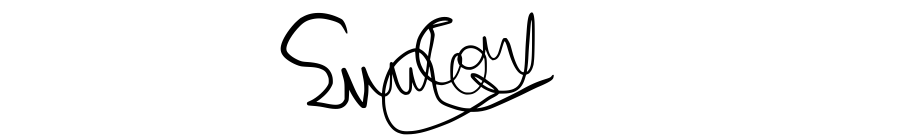
\includegraphics[height=0.8cm]{signature.png}\\[-3pt]
\end{flushleft}
}

\title{
  \vspace{-30mm}
  \begin{spacing}{1.0}
    \huge\textbf{\thesisTitle}
  \end{spacing}
  \logo\\[-5mm]
  \LARGE{\thesisMyName}\\
  \large{\thesisDepartmentName\\University of Exeter}\\[8mm]
  \statement
}
\author{}
\date{}

% =========================================================
% Chapter heading style
% =========================================================
\makeatletter
\def\@makechapterhead#1{%
  \vspace*{40\p@}%
  {\parindent \z@ \raggedright \normalfont
    \interlinepenalty\@M
    \Huge \bfseries
    \ifnum \c@secnumdepth >\m@ne
      \thechapter.\nobreakspace
    \fi
    #1\par\nobreak
    \vskip 40\p@
  }}
\makeatother

% =========================================================
% Blank page helper
% =========================================================
\newcommand\blankpage{
  \null
  \thispagestyle{empty}
  \addtocounter{page}{-1}
  \newpage
}
% =========================================================
% Document
% =========================================================

\begin{document}

% ---------- Front matter ----------
\frontmatter
\maketitle
\cleardoublepage
% \pagenumbering{arabic}
% \setcounter{page}{1}
\chapter*{Abstract}

Graphs arise in many scientific and computational domains, ranging from social networks to biology and chemistry. Their
irregular, non-Euclidean structure makes them expressive, but also difficult to
represent, generate, and evaluate. This thesis develops robust and
interpretable methods for graph representation, conditional graph generation,
and statistically grounded evaluation of graph generative models.

The first contribution is the Neighborhood Subgraph Pairwise Path Kernel
(NSPPK), an explicit graph kernel for attributed graphs. NSPPK represents a
graph using pairs of local subgraphs centred on selected anchor nodes, together
with the graph regions that connect those anchors. The connector subgraphs are
constructed from unions of shortest paths between the anchor nodes, allowing
the kernel to capture both the structure surrounding each anchor and the
structure linking different parts of the graph. NSPPK also incorporates
continuous node attributes directly into its feature map, avoiding
discretisation while preserving a sparse, deterministic, and interpretable
representation. Experiments show that NSPPK performs competitively with
established graph kernels and graph neural networks while offering strong
sample efficiency and computational transparency.

The second contribution is the Graph-Conditioned Diffusion Generator (GCDG), a
conditional diffusion-based graph generator that uses graph-level feature
vectors to guide the generation of node-level features before constructing a
final discrete graph. Its central focus is the graph-level-to-node-level
generation problem: translating a global graph descriptor into node existence,
node labels, degree information, and pairwise edge structure. The model
separates continuous diffusion-based denoising, node and edge prediction, and
constraint-aware decoding. This design makes intermediate predictions
inspectable and allows graph feasibility constraints to be enforced explicitly
during decoding. Experiments on synthetic graph families and QM9-like molecular
graphs show that conditional graph generation should be evaluated not only by
the realism of the generated graphs, but also by how faithfully they preserve
the information encoded in the conditioning vectors.

The third contribution is RankGen, a statistically grounded framework for
generative model evaluation. RankGen treats evaluation as a set of predictive
probes rather than as a single scalar similarity score. It defines
complementary metrics for Quality, Utility, Indistinguishability, and
Similarity, combines them with PAC-style reliability bounds, and ranks
generators using robust quantile-based summaries. Experiments across
controlled perturbations, molecular graph generators, image benchmarks, and
open-domain text generation demonstrate that RankGen can diagnose failure
modes such as memorisation, mode collapse, poor augmentation value, and
distributional mismatch.

Together, these contributions support a unified view of graph generative
modelling: reliable generation requires graph representations that expose
meaningful structure, generative models whose outputs can be explicitly
conditioned, and evaluation protocols that distinguish genuine task-relevant
utility from superficial structural similarity.

\cleardoublepage
\chapter*{Acknowledgements}



I would like to express my deepest gratitude to my first supervisor Dr Fabrizio Costa and my second supervisor Professor Jonathan Fieldsend for their support, guidance and encouragement throughout this thesis. Their insight, patience and belief in my work have been invaluable. This thesis would not have been possible without their supervision, and I owe nearly all of my progress to them.

I am also profoundly grateful to my mentor and lifelong friend, Dr Döndü Sarışen, who has been part of my journey from beginning to end. Her wisdom, and friendship have meant more to me than words can express.
I would also like to thank my friend Cai Heng for her support and encouragement throughout this process.

Along the way, I have had the privilege of meeting many wonderful people who have contributed to this journey in different ways. In particular, I would like to thank Dr Mohammad Hajsadeghi and his wife, whose example of family, kindness, and integrity has left a lasting impression on me. I am also grateful to Alexandru Anton for the occasional walks around campus and the thoughtful conversations on literature and life that accompanied them during the very early stages of my PhD.

Finally, I would like to thank my family for their love, patience, and support. Above all, I give thanks to Mother Mary and to God, whose grace and guidance have carried me through this journey.


\epigraph{I am incapable of describing the feeling with which I left. I would not want it ever to be repeated, but I would have considered myself unfortunate if I had never experienced it.}
{\normalsize --- \textup{Ivan Turgenev}}


\addcontentsline{toc}{chapter}{List of Publications}
\chapter*{List of Publications}

\section*{Manuscripts Under Review}

\begin{enumerate}
    \item Cosmina Simionescu and Fabrizio Costa.
    \textit{Fast, Sparse, and Accurate Kernels for Node-Attributed Graphs}.
    NeurIPS 2026 Conference submission, under review.

    \item Cosmina Simionescu and Fabrizio Costa.
    \textit{GUIDE: A Task-Grounded Diagnostic Protocol for Generative Model Evaluation}.
    NeurIPS 2026 Conference submission, under review.
\end{enumerate}




\tableofcontents
\listoffigures
\listoftables
\listofalgorithms

\cleardoublepage
\chapter*{List of Notation}
\addcontentsline{toc}{chapter}{List of Notation}

\small
\setlength{\tabcolsep}{3pt}
\renewcommand{\arraystretch}{1.00}
\setlength{\extrarowheight}{0pt}

% left column width
\newcolumntype{L}{>{\raggedright\arraybackslash}p{0.28\textwidth}}

% section header row
\newcommand{\notsec}[1]{%
  \addlinespace[0.35em]
  \multicolumn{2}{@{}l@{}}{\textbf{#1}}\\[-0.2em]
  \midrule
}

\begin{tabularx}{\textwidth}{@{}L X@{}}
\toprule

\notsec{Graphs and matrices}
$G=(V,E)$ & Graph with node set $V$ and edge set $E$ \\
$V$ & Set of vertices (nodes), $V=\{v_1,\dots,v_n\}$ \\
$E$ & Set of edges (undirected: $\{u,v\}$; directed: $(u,v)$) \\
$n$ & Number of nodes in a graph ($n=|V|$) \\
$m$ & Number of edges in a graph ($m=|E|$) \\
$A \in \mathbb{R}^{n\times n}$ & Adjacency matrix ($A_{ij}=1$ if $(v_i,v_j)\in E$, else $0$; in weighted graphs, $A_{ij}$ stores the edge weight, while neighbourhoods are defined by edge incidence unless stated otherwise) \\
$D \in \mathbb{R}^{n\times n}$ & Degree matrix (diagonal with $D_{ii}=\sum_j A_{ij}$) \\
$L$ & (Unnormalised) graph Laplacian ($L=D-A$) \\
$L_{\mathrm{sym}}$ & Symmetric normalised Laplacian ($L_{\mathrm{sym}}=I-D^{-1/2}AD^{-1/2}$, when defined) \\
$d(u,v)$ & Shortest-path distance between nodes $u$ and $v$ \\
$\mathcal{N}(v)$ & 1-hop neighbourhood of $v$ ($\mathcal{N}(v)=\{u\in V:(u,v)\in E\}$) \\
$N_r(v)$ & $r$-hop neighbourhood vertex set of $v$ ($N_r(v)=\{u\in V:d(u,v)\le r\}$); when used as a feature component, it denotes the rooted induced subgraph on this set \\
$\deg(v)$ & Degree of node $v$ ($\deg(v)=|\mathcal{N}(v)|$) \\
$\deg^*$ & Maximum degree of $G$ ($\deg^*=\max_{v\in V}\deg(v)$) \\
$G[S]$ & Subgraph of $G$ induced by the vertex subset $S\subseteq V$ \\

\notsec{Attributes and representations}
$d_x$ & Dimension of node attributes \\
$d_e$ & Dimension of edge attributes \\
$x_v \in \mathbb{R}^{d_x}$ & Node attribute (feature vector) of node $v$ \\
$X \in \mathbb{R}^{n \times d_x}$ & Node-attribute matrix (row $i$ is $x_{v_i}^{\top}$) \\
$e_{uv} \in \mathbb{R}^{d_e}$ & Edge attribute (feature vector) on edge $(u,v)$, if present \\
$\phi:\mathcal{G}\to\mathbb{R}^d$ & Graph-to-vector representation map (explicit or learned) \\
$z=\phi(G)\in\mathbb{R}^d$ & Graph embedding of $G$ \\

\notsec{Permutation symmetry}
$\pi$ & Permutation of $\{1,\dots,n\}$ (vertex relabeling) \\
$P_\pi \in \{0,1\}^{n\times n}$ & Permutation matrix corresponding to $\pi$ \\
$A^\pi$ & Relabelled adjacency: $A^\pi = P_\pi A P_\pi^\top$ \\
$X^\pi$ & Relabelled node features: $X^\pi = P_\pi X$ \\

\notsec{Kernels and RKHS}
$k(\cdot,\cdot)$ & Kernel (similarity) function \\
$\phi_k(\cdot)$ & Kernel feature map ($k(x,x')=\langle \phi_k(x),\phi_k(x')\rangle_{\mathcal{H}_k}$) \\
$\mathcal{H}_k$ & Reproducing kernel Hilbert space (RKHS) associated with kernel $k$ \\
$K \in \mathbb{R}^{N\times N}$ & Gram (kernel) matrix with $K_{ij}=k(x_i,x_j)$ \\

\notsec{NSPPK feature construction}
$U(u,v)$ & Subgraph induced by the union of all shortest paths between anchor nodes $u$ and $v$ \\
$C_{r'}(u,v)$ & Connector subgraph obtained by expanding $U(u,v)$ by radius $r'$ \\
$b$ & Number of hash bits used in feature hashing \\
$M=2^b$ & Number of hash buckets in the finite hash codomain \\
$H_b(\cdot)$ & $b$-bit base hash function \\
$H^q(\cdot)$ & Sequence hash for ordered tuples \\
$H^t(\cdot)$ & Multiset hash for unordered collections \\
$f_G^\theta$ & Sparse NSPPK feature-count vector for graph $G$ with parameters $\theta$ \\
$\theta=(R,D,R')$ &
NSPPK feature-extraction parameters: maximum anchor-neighbourhood radius,
maximum anchor distance, and maximum connector radius \\

\notsec{GNNs: message passing and readout}
$\ell$ & Layer index (for neural networks / GNNs) \\
$L_{\mathrm{GNN}}$ & Number of GNN layers \\
$\mathbf{h}_v^{(\ell)}$ & Hidden state (embedding) of node $v$ at layer $\ell$ \\
$\mathbf{m}_v^{(\ell)}$ & Aggregated message for node $v$ at layer $\ell$ \\
$\psi^{(\ell)}(\cdot)$ & Message function at layer $\ell$ \\
$\phi^{(\ell)}(\cdot)$ & Update function at layer $\ell$ \\
$\mathrm{AGG}^{(\ell)}(\cdot)$ & Permutation-invariant aggregation (sum/mean/max/attention) \\
$\mathrm{READOUT}(\cdot)$ & Permutation-invariant pooling/readout to obtain a graph embedding \\
$\mathbf{z}_G$ & Graph-level embedding produced by readout \\

\notsec{Graph Transformers}
$X\in\mathbb{R}^{n\times d}$ & Input token/node embedding matrix to attention \\
$\mathbf{Q},\mathbf{K},\mathbf{V}$ & Query/key/value projections \\
$\mathbf{a}_{ij}$ & Attention weight from token $i$ to token $j$ \\
$H$ & Number of attention heads \\

\notsec{Diffusion models}
$x_0$ & Clean data sample (e.g., graph representation) \\
$x_t$ & Noised latent variable at diffusion step $t$ \\
$T$ & Total number of diffusion steps \\
$\beta_t$ & Forward noise schedule parameter at step $t$ \\
$\alpha_t$ & $\alpha_t=1-\beta_t$ \\
$\bar{\alpha}_t$ & Cumulative product $\bar{\alpha}_t=\prod_{s=1}^t \alpha_s$ \\
$\varepsilon$ & Standard Gaussian noise, $\varepsilon\sim\mathcal{N}(0,I)$ \\
$\varepsilon_\theta(x_t,t)$ & Neural noise predictor (denoiser) \\
$p_\theta(x_{t-1}\mid x_t)$ & Learned reverse transition kernel \\
$q(x_t\mid x_{t-1})$ & Forward noising transition kernel \\

\notsec{Graph-conditioned denoising generator}
$N_{\max}$ & Maximum number of node rows in the padded node-feature matrix \\
$K_V=|\mathcal{T}_V|$ & Number of node-label classes \\
$\tau_V,\tau_E$ & Node-label and edge-label functions, respectively \\
$C\in\mathbb{R}^{d_C}$ & Graph-level condition vector supplied to the generator \\
$d_C$ & Dimension of the graph-level condition vector \\
$r_i\in\mathbb{R}^{d_r}$ & Node-level structural representation for node row $i$ \\
$d_r$ & Dimension of the node-level structural representation \\
$m_i$ & Node-existence indicator for row $i$ \\
$g_i$ & Degree component or degree class associated with row $i$ \\
$q_i$ & One-hot node-label vector for row $i$ \\
$d_{\mathrm{feat}}$ & Dimension of each node-feature row \\
$X_0$ & Clean padded node-feature matrix \\
$X_t$ & Noisy node-feature matrix at noise level or diffusion time $t$ \\
$\sigma(t)$ & Noise scale at time $t$ \\
$\Gamma(t)$ & Feature-wise noise-scale matrix used in the corruption process \\
$Z$ & Node-latent matrix produced by the conditional denoising network \\
$z_i$ & Latent representation of node row $i$ \\
$B_{\mathrm{match}}$ & Feature mask used in matched-row training loss \\
$\pi^\star$ & Minimum-cost row assignment used for matched-row loss \\
$P^{\mathrm{edge}}$ & Predicted edge-probability matrix passed to the graph decoder \\
$A_t^{\mathrm{state}}$ & Provisional edge-state matrix used by the joint edge-state variant \\

\notsec{Learning theory and evaluation}
$\mathcal{X},\mathcal{Y}$ & Input and label spaces \\
$P$ & Data-generating distribution over $\mathcal{X}\times\mathcal{Y}$ \\
$S$ & Finite sample drawn i.i.d.\ from $P$ \\
$N_{\mathrm{sample}}$ & Sample size in learning-theory or evaluation contexts \\
$\mathcal{H}$ & Hypothesis class (models/predictors) \\
$h\in\mathcal{H}$ & Hypothesis/model \\
$\ell(\cdot,\cdot)$ & Loss function \\
$R_P(h)$ & Population risk (expected loss) under $P$ \\
$\widehat{R}_S(h)$ & Empirical risk on sample $S$ \\
$\delta$ & Confidence parameter in PAC bounds \\
$\epsilon_{\mathrm{PAC}}$ & Accuracy or estimation-error parameter in PAC-style bounds \\
$\mathfrak{R}_S(\mathcal{H})$ & Empirical Rademacher complexity \\
$d_{\mathrm{VC}}$ & VC dimension (binary classification) \\
$P,Q$ & Distributions over inputs (e.g., real vs.\ generated) \\
$\mathrm{disc}_{\mathcal{H}\Delta\mathcal{H}}(P,Q)$ & Discrepancy between $P$ and $Q$ with respect to $\mathcal{H}\Delta\mathcal{H}$ \\
$\lambda(P,Q)$ & Joint optimal risk term in domain adaptation bounds \\
$\mathrm{MMD}(\mathcal{X},\mathcal{Y})$ & Maximum Mean Discrepancy between sample sets $\mathcal{X}$ and $\mathcal{Y}$ \\
$\rho_i$ & Classifier-based evaluation metric (defined in Chapter~\ref{ch:rankgen}) \\

\notsec{RankGen evaluation}
$D_{\text{train1}}^{(i)}$ & Real training subset used for the baseline classifier on split $i$ \\
$D_{\text{train2}}^{(i)}$ & Additional real training subset used for the upper-bound classifier on split $i$ \\
$D_{\text{generated}}^{(i)}$ & Generated dataset used on split $i$ \\
$D_{\text{test}}$ & Held-out real test set used for evaluation \\
$\Phi_\theta$ & Task classifier used in classifier-based evaluation probes \\
$\Psi_\theta$ & Binary discriminator for real-versus-generated evaluation \\
$\Gamma_\theta$ & Similarity or neighbourhood-mixing probe used in RankGen \\
$\rho_1,\ldots,\rho_6$ & Raw classifier-derived scores used to define RankGen metrics \\
$Q^{(i)}$ & Quality score on split $i$ \\
$U^{(i)}$ & Utility score on split $i$ \\
$I^{(i)}$ & Indistinguishability score on split $i$ \\
$S^{(i)}$ & Similarity score on split $i$ \\
$\mathcal{E}_{\min}^{(i)}$ & Exchangeability score on split $i$ \\

\bottomrule
\end{tabularx}

\normalsize

\glsaddall[types=\acronymtype]
\printglossary[type=\acronymtype, title={List of Abbreviations}, toctitle={List of Abbreviations}]

% Optional: print terms glossary too (uncomment if you want it)
% \printglossary[title={Glossary of Terms}, toctitle={Glossary of Terms}]

\afterpage{\blankpage}

% ---------- Main matter ----------
\mainmatter


% Graph definitions and foundational notation are now given in Chapter~\ref{ch:theory}.
% The old ch-1/glossary include is disabled because that file is not present.
% \include{ch-1/glossary}

\chapter{Introduction}
\label{ch:intro}

\section{Motivation}
\label{sec:intro:motivation}

Graphs arise across a wide range of scientific and technological domains. Molecules can be represented as atoms connected by chemical bonds; citation networks as documents linked by references; social networks as individuals connected through interactions; and biological systems as proteins, genes, or metabolites related through functional processes. More generally, many complex systems are naturally described as collections of entities together with the relationships among them. In these settings, the graph is not merely a convenient storage format: its connectivity is an essential part of the object being modelled.

This thesis studies three closely connected problems in graph machine learning:
how to construct graph representations that expose structural information, how
to generate new graphs under graph-level conditions, and how to evaluate graph
generative models with explicit reliability checks. Although these problems are
often considered separately, they influence one another. A generative model can
only be guided by information that has been represented effectively; generated
graphs can only be trusted when their quality and task-relevant utility can be
assessed; and such assessments depend on representations that expose the
structural properties of interest.

Graph data present challenges that distinguish them from vectors, images, and sequences. Graphs have no canonical ordering of their nodes, may vary substantially in size, and often contain irregular local structures~\citep{bronstein2017geometric}. Their defining properties may depend on small motifs, extended neighbourhoods, or long-range connectivity across distant regions. These characteristics motivate expressive learning methods such as graph neural networks and graph diffusion models, but they also complicate interpretability, robustness, and evaluation.

Graph kernels provide a complementary approach to learning from graph-struc\-tured data. Over the past two decades, numerous kernels have been developed to compare graphs through structural components such as walks, paths, neighbourhoods, subtrees, and graphlets~\citep{nikolentzos2021graph}. Their explicit and deterministic representations can support feature-level inspection and sample efficiency. However, many classical graph kernels were designed primarily for discrete node labels and therefore handle continuous attributes only through discretisation or other indirect mechanisms. Neural approaches can learn more flexible representations from attributed data, but their behaviour may be sensitive to optimisation and architectural choices and can be more difficult to inspect.

This thesis is motivated by the view that reliable graph machine learning should combine the strengths of these traditions. It develops explicit representations that retain meaningful graph structure, conditional generative models whose outputs can be guided by graph-level information, and evaluation protocols that distinguish genuine structural and task-relevant utility from superficial similarity.


\section{Problem Setting}
\label{sec:intro:problem}

The central object considered in this thesis is a graph
\[
    G=(V,E),
\]
possibly equipped with node labels, edge labels, or continuous node attributes.
The thesis focuses on graph-level and dataset-level questions rather than on a
single supervised prediction task. In particular, it considers:

\begin{enumerate}[label=(\roman*)]
    \item representation: constructing graph feature maps that preserve
    structural and attribute information while remaining computationally
    practical and interpretable;
    \item generation: producing labelled graphs from graph-level conditioning
    information using a staged denoising and decoding process; and
    \item evaluation: comparing generative models using diagnostic,
    statistically controlled measures rather than relying on a single heuristic
    score.
\end{enumerate}

These three components form the methodological arc of the thesis, but they
should not be read as a single mandatory end-to-end system. The contributions
are operationally independent: NSPPK is a graph representation method, GCDG is
a graph-conditioned generator, and RankGen is a general diagnostic evaluation
framework. They address successive decisions that arise in graph generative
modelling: what graph information is represented, how such information can
condition generation, and how generated data should be assessed.

\section{Aim, Objectives, and Research Questions}
\label{sec:intro:questions}

The overall aim of this thesis is to develop graph representation,
graph-conditioned generation, and diagnostic evaluation methods that are
explicit about structural information, conditioning behaviour, and the
reliability of empirical comparisons.

This aim is addressed through the following objectives.

\begin{description}[leftmargin=0pt,style=nextline]
    \item[O1.]
    To develop an explicit graph representation whose individual features jointly encode the local neighbourhoods around node pairs and the longer-range structure connecting them, while incorporating continuous node attributes without discretisation.
    \item[O2.]
    To evaluate whether such an explicit representation can provide accurate,
    scalable, and interpretable graph-level features across molecular,
    citation, and larger-scale graph benchmarks.

    \item[O3.]
    To design a graph-conditioned diffusion generator that uses graph-level
    structural information to guide the generation of discrete graphs.

    \item[O4.]
    To separate node-level diffusion, edge prediction, and constraint-aware
    decoding so that the graph generation process is inspectable and can
    incorporate feasibility constraints.

    \item[O5.]
    To develop a diagnostic evaluation framework that compares generative
    models with reliability checks and diagnoses multiple generative failure
    modes, including poor task fidelity,
    distributional mismatch, low augmentation value, local structural
    mismatch, and memorisation.

    \item[O6.]
    To compare generative models using uncertainty-aware summaries and
    reliability checks rather than relying only on single scalar metrics.
\end{description}

These objectives lead to the following research questions.

\begin{description}[leftmargin=0pt,style=nextline]
    \item[RQ1.]
    How can graph kernels be extended to incorporate continuous node attributes
    directly while retaining explicit, sparse, and interpretable feature maps?

    \item[RQ2.]
    How can graph-level structural information be used to condition a
    diffusion-based generator for labelled graphs?

    \item[RQ3.]
    How can graph generative models be evaluated in a way that distinguishes
    predictive utility, distributional alignment, memorisation, and structural
    fidelity?

    \item[RQ4.]
    How can empirical generator comparisons be made more reliable through
    uncertainty-aware summaries and statistical guarantees?
\end{description}

These questions are deliberately connected. The first question concerns the
representation of graph structure. The second uses such representations as
conditioning signals for generation. The third and fourth address the problem
of deciding whether generated samples should be trusted.

\begin{table}[t]
\centering
\footnotesize
\begin{tabularx}{\textwidth}{@{}l l l X@{}}
\toprule
Research question & Objectives & Chapter & Evidence \\
\midrule
RQ1 & O1--O2 & Chapter~\ref{ch:nsppk} &
Kernel construction, feature analysis, classification experiments, scalability
tests, and interpretability analysis. \\
RQ2 & O3--O4 & Chapter~\ref{ch:generator} &
Synthetic cycle--leg generation, conditional decoding diagnostics, ablations,
and QM9 molecular experiments. \\
RQ3 & O5 & Chapter~\ref{ch:rankgen} &
Quality, Utility, Indistinguishability, Similarity, and memorisation-sensitive
diagnostics across controlled perturbations and generative benchmarks. \\
RQ4 & O6 & Chapter~\ref{ch:rankgen} &
PAC-style reliability checks, repeated resampling, quantile summaries, and
model ranking analyses. \\
\bottomrule
\end{tabularx}
\caption{Mapping between research questions, objectives, thesis chapters, and
the main evidence used to answer each question.}
\label{tab:intro:rq-objective-map}
\end{table}

\section{Thesis Contributions}
\label{sec:intro:contributions}

This thesis makes three main methodological contributions.

\textbf{Explicit attributed graph representation.}
Chapter~\ref{ch:nsppk} introduces the Neighborhood Subgraph Pairwise Path
Kernel (NSPPK), an explicit graph kernel whose features jointly encode the
local neighbourhoods around node pairs and the broader graph structure
connecting them. Connector subgraphs are constructed from unions of shortest
paths, while continuous node attributes are incorporated directly into the
feature map without discretisation. The resulting representation is sparse,
deterministic, and interpretable, supports efficient dot-product kernel
evaluation, and allows predictive signals to be traced back to structural
graph patterns.

\textbf{Graph-conditioned Diffusion generation.}
Chapter~\ref{ch:generator} introduces the Graph-Conditioned Diffusion Generator
(GCDG), a conditional generator that separates continuous node-level denoising
from discrete graph construction. A graph-level condition vector guides a
transformer-based denoising model, while node existence, node and edge labels,
degrees, and edge probabilities are predicted through dedicated modules before
constraint-aware decoding. This staged design makes intermediate predictions
inspectable and allows graph feasibility constraints to be enforced explicitly
during generation.

\textbf{Statistically grounded generator evaluation.}
Chapter~\ref{ch:rankgen} introduces RankGen, a classifier-based framework for
evaluating generative models. RankGen defines complementary measures of
Quality, Utility, Indistinguishability, and Similarity, each designed to expose
a different failure mode. It combines these measures with PAC-style reliability
bounds, robust quantile summaries, and a ranking procedure that distinguishes
statistical confidence from fine-grained model comparison. The framework is
validated across controlled perturbations and generative tasks involving
molecular graphs, images, and open-domain text.

Together, these contributions support a qualified central claim: graph
generation benefits from treating representation, synthesis, and diagnosis as
connected design decisions. This is a methodological perspective rather than a
claim that the thesis evaluates one fully integrated system throughout. In the
reported generator experiments, graph-level descriptors are used to condition
GCDG; RankGen is developed as a broader diagnostic framework for evaluating
generated data rather than as an optimiser inside the generator. Generated
graphs should therefore not be judged using a single measure of plausibility,
but according to whether they preserve relevant structure, satisfy domain
constraints, support downstream use, and pass the reliability checks required
by the evaluation setting.

\section{Thesis Structure}
\label{sec:intro:structure}

Chapter~\ref{ch:theory} introduces the theoretical and methodological
background required for the thesis, including graph notation, graph
representation learning, graph kernels, neural graph models, diffusion-based
generation, and principles for evaluating generated data.

Chapter~\ref{ch:nsppk} develops NSPPK and presents its construction,
computational analysis, implementation, and empirical evaluation.

Chapter~\ref{ch:generator} develops GCDG and describes its conditioning
mechanism, corruption and diffusion processes, prediction modules, decoding
procedure, training objective, and empirical evaluation.

Chapter~\ref{ch:rankgen} develops RankGen, defines its evaluation measures and
reliability guarantees, and assesses the framework on molecular graphs, images,
and open-domain text, as well as under controlled perturbation settings.

Chapter~\ref{ch:conclusion} summarises the findings, discusses the limitations
of the proposed methods, and outlines directions for future research.

\chapter{Theory and Foundations}
\label{ch:theory}

This chapter establishes the theoretical foundations that underpin the three
core contributions of this thesis: interpretable graph representations,
diffusion-based graph generation, and statistically grounded generative model
evaluation.
We begin by introducing the mathematical representation of graphs enriched with structural
and attribute information, toghether with the mathematical notation used
throughout the thesis. Fundamental concepts including permutation invariance,
matrix representations, and neighbourhood structures are presented to clarify
the computational and symmetry properties that distinguish graphs from
Euclidean data.

Building on this foundation, we review the principal paradigms of graph
representation learning, distinguishing between predefined
(data-independent) representations and learned (data-driven) embeddings.
This unified perspective situates graph kernels and neural models within a
common framework and highlights their complementary strengths.
We then survey modern deep generative models for graphs, with particular
emphasis on diffusion-based approaches and the challenges posed by the  
discrete structure of the graphs, permutation symmetry, and structural validity
constraints. Finally, we examine existing methodologies for evaluating generative models
and introduce learning-theoretic tools that enable statistically grounded and
reliable model comparison.Together, these components provide the conceptual, mathematical, and
methodological framework required for the developments presented in the
subsequent chapters.

\section{Graphs and Structured Data}


Graphs are a fundamental data structure for modeling relationships among entities
and arise naturally in a wide range of application domains, including social
networks~\citep{newman2003structure}, bioinformatics~\citep{borgwardt2005protein},
chemoinformatics~\citep{weininger1988smiles}, recommender systems~\citep{ying2018graph},
and cybersecurity~\citep{10.1145/310889.310919}. Unlike data embedded in regular
Euclidean domains such as images or sequences, graphs encode irregular,
non-Euclidean structures with variable neighbourhood sizes and complex
topologies~\citep{bronstein2017geometric}. This structural flexibility makes graphs
a powerful modeling formalism, but also introduces significant challenges for
representation, learning, generation, and evaluation.
\begin{definition}[Graph]
A (finite) graph is a tuple $G=(V,E)$, where
$V=\{v_1,\dots,v_n\}$ is a set of vertices and
$E \subseteq V \times V$ is a set of edges.
If $G$ is \emph{undirected}, edges are unordered pairs $\{u,v\}$; if
$G$ is \emph{directed}, edges are ordered pairs $(u,v)$.
\end{definition}
\begin{definition}[Graph isomorphism]
Two graphs $G=(V,E)$ and $G'=(V',E')$ are said to be \emph{isomorphic}
if there exists a bijection $\pi: V \to V'$ such that
\[
(u,v) \in E \iff (\pi(u),\pi(v)) \in E'.
\]
Graph isomorphism formalizes structural equivalence independently of
vertex ordering.
\end{definition}
\begin{figure}[h]
\centering
\begin{tikzpicture}[
  x=1cm,y=1cm,
  vnode/.style={circle,draw,minimum size=5mm,inner sep=0pt},
 % bigger circles
  edge/.style={line width=0.6pt},
  lab/.style={font=\small} % labels slightly larger
]

% ---------------- (a) undirected ----------------
\begin{scope}
  \node[vnode] (a1) at (0,1) {};
  \node[vnode] (b1) at (2,1) {};
  \node[vnode] (c1) at (2,0) {};
  \node[vnode] (d1) at (0,0) {};

  \draw[edge] (a1)--(b1);
  \draw[edge] (b1)--(c1);
  \draw[edge] (c1)--(d1);
  \draw[edge] (a1)--(c1);
      \draw[edge] (a1)--(d1);


  % no labels in (a), like your picture
\end{scope}

% ---------------- (b) labeled ----------------
\begin{scope}[xshift=4.2cm]
  \node[vnode] (a2) at (0,1) {};
  \node[vnode] (b2) at (2,1) {};
  \node[vnode] (c2) at (2,0) {};
  \node[vnode] (d2) at (0,0) {};

  % edges with labels
  \draw[edge] (a2)-- node[lab, above=4pt] {$\ell_1$} (b2);
  \draw[edge] (b2)-- node[lab, right=4pt] {$\ell_2$} (c2);
  \draw[edge] (c2)-- node[lab, below=4pt] {$\ell_3$} (d2);
  \draw[edge] (a2)-- node[lab, left=4pt] {$\ell_4$} (d2);
  \draw[edge] (a2)-- node[lab, sloped, above=-1pt] {$\ell_5$} (c2);

  % node labels OUTSIDE, farther away
  \node[lab, above=10pt] at (a2) {$a$};
  \node[lab, above=10pt] at (b2) {$b$};
  \node[lab, below=10pt] at (d2) {$c$};
  \node[lab, below=10pt] at (c2) {$d$};
\end{scope}
% ---------------- (c) real-valued attributed ----------------
\begin{scope}[xshift=8.4cm]
  \node[vnode] (a3) at (0,1) {};
  \node[vnode] (b3) at (2,1) {};
  \node[vnode] (c3) at (2,0) {};
  \node[vnode] (d3) at (0,0) {};

  \draw[edge] (a3)--(b3);
  \draw[edge] (b3)--(c3);
  \draw[edge] (c3)--(d3);
  \draw[edge] (a3)--(c3);
    \draw[edge] (a3)--(d3);


  % attribute labels OUTSIDE (like your picture) and farther away
  \node[lab, above=10pt] at (a3) {$(1,3,0)$};
  \node[lab, above=10pt] at (b3) {$(0,2,5)$};
  \node[lab, below=10pt] at (d3) {$(1,1,2)$};
  \node[lab, below=10pt] at (c3) {$(2,0,4)$};
\end{scope}

\end{tikzpicture}
\caption{(a) Unlabelled undirected graph. (b) Fully labeled graph (node and edge labels). (c) Attributed graph with real-valued node features.}
\label{fig:graph-types}
\end{figure}
In many real-world settings, graph structure alone is insufficient to fully
characterize the objects of interest. Nodes and edges are often associated with
additional information, such as atom types and charges in molecular graphs,
user profiles in social networks, or transaction metadata in cybersecurity
applications. This motivates the use of graphs augmented with label or attribute
information.

A graph whose vertices are assigned discrete labels is referred to as a
\emph{node-labeled} graph, while a graph whose edges carry labels is termed
\emph{edge-labeled}. When both vertices and edges are labeled, the graph is
\emph{discretely labeled}. Figure~\ref{fig:graph-types} illustrates several common
graph variants considered in this thesis, including an undirected graph, a fully
labeled graph, and a graph with real-valued node attributes.

\begin{definition}[Labeled graph]
A labeled graph is a graph $G=(V,E)$ equipped with a labeling function
$\ell: V \to \mathcal{L}$ and, optionally, an edge labeling function
$\ell_E: E \to \mathcal{L}_E$, where $\mathcal{L}$ and $\mathcal{L}_E$ are finite
sets of discrete labels.
\end{definition}
\footnote{Unless stated otherwise, all graphs considered in this thesis are simple graphs: they do not contain parallel edges or self-loops.}
In many applications, however, vertex and edge annotations are not restricted to
single discrete labels but take the form of feature vectors encoding multiple
categorical or real-valued properties. Graphs endowed with such vector-valued
annotations are known as \emph{attributed graphs}.

\begin{definition}[Attributed graph]
 An attributed graph is a graph $G=(V,E)$
equipped with node and, optionally, edge attributes. Let $d_x$ and $d_e$ denote
the dimensions of node and edge attributes, respectively. Node attributes are
specified by a function $x: V \to \mathbb{R}^{d_x}$, assigning a feature vector
$x_v$ to each node $v$, and edge attributes by a function
$e: E \to \mathbb{R}^{d_e}$, assigning a feature vector $e_{uv}$ to each edge
$(u,v)$. Attributes may be continuous or categorical.
\end{definition} 
We assume a fixed ordering of the vertex set $V=\{v_1,\dots,v_n\}$.
Under this ordering, the adjacency matrix provides a canonical matrix
representation of the graph structure and consists of $n$ rows and $n$ columns,
that is, $A\in\mathbb{R}^{n\times n}$.
For a vertex $v_i\in V$, its (open) neighbourhood is defined as
\[
N(v_i)=\{\,v_j\in V \mid (v_i,v_j)\in E\,\},
\]
that is, the set of vertices adjacent to $v_i$.
The degree of $v_i$ in $G$, denoted by $\deg_G(v_i)$, is the cardinality of its
neighbourhood, $\deg_G(v_i)=|N(v_i)|$.
These notions capture basic local structural properties and will be used
throughout this thesis.

\begin{definition}[Adjacency matrix]
Let $G=(V,E)$ be a graph with $|V|=n$ and a fixed vertex ordering.
The adjacency matrix $A\in\mathbb{R}^{n\times n}$ is defined by
$A_{ij}=1$ if $(v_i,v_j)\in E$ and $A_{ij}=0$ otherwise; for weighted graphs,
$A_{ij}$ may store an edge weight.
\end{definition}

\paragraph{Neighborhood and degree.}
For a vertex $v_i\in V$, the (open) neighbourhood is
\[
N(v_i)=\{\,v_j\in V \mid (v_i,v_j)\in E\,\}.
\]
The degree of $v_i$ in $G$, denoted $\deg(v_i)$, is the number of adjacent
vertices,
\[
\deg(v_i)=|N(v_i)|.
\]
The maximum degree of $G$ is $\deg^*=\max_{v\in V}\deg(v)$.
\paragraph{Laplacian matrix.}
Let $A$ be the adjacency matrix of $G=(V,E)$ and let
$D\in\mathbb{R}^{n\times n}$ be the diagonal degree matrix with
$D_{ii}=\sum_j A_{ij}$.
The (unnormalised) graph Laplacian is defined as
\[
L=D-A.
\]
\paragraph{Subgraphs.}
A graph $G'=(V',E')$ is a subgraph of $G=(V,E)$ if $V'\subseteq V$ and
$E'\subseteq E$.
Given a vertex subset $S\subseteq V$, the induced subgraph $G(S)$ is defined as
\[
\begin{aligned}
G(S) &= (S,E(S)), \\
E(S) &= \{(u,v)\in E \mid u,v\in S\}.
\end{aligned}
\]
\paragraph{Shortest paths and neighborhoods.}
Let $G=(V,E)$ be a graph and let $u,v\in V$ belong to the same connected
component. A \emph{path} between $u$ and $v$ is a sequence of adjacent vertices
connecting them. Among all such paths, there exists at least one with minimal
length, measured as the number of edges it contains; this follows from the
finiteness of the graph. The \emph{shortest-path distance} $d(u,v)$ is defined as
the length of such a shortest path. While multiple shortest paths may exist
between two vertices, their length is unique.

In weighted graphs, the distance $d(u,v)$ is defined as the minimum total weight
along any path connecting $u$ and $v$. Distances of this form are well defined
whenever edge weights are non-negative, and can be computed in polynomial time
using classical algorithms such as Dijkstra's algorithm \citep{dijkstra1959note}.


The notion of shortest-path distance induces a metric structure on each
connected component of the graph. This, in turn, gives rise to the concept of
local neighbourhoods. For a vertex $v \in V$ and radius $r \geq 0$, the radius-$r$ neighbourhood of $v$ is defined as
\[
N_r(v)=\{u \in V \mid d(u,v) \leq r\}.
\]
For unweighted graphs, this corresponds to the usual $r$-hop neighbourhood when
$r$ is an integer.
These neighborhoods capture increasingly large local regions of the graph and
play a central role in many graph representation, learning, and kernel-based
methods.
\paragraph{Permutation invariance and equivariance.}
A central challenge in learning on graphs is that vertex identities are
arbitrary: a relabeling of the vertices should not change the underlying
graph. Formally, let $n=|V|$ and let $\pi$ be a permutation of $\{1,\dots,n\}$.
We represent $\pi$ by its permutation matrix $P_\pi\in\{0,1\}^{n\times n}$.
If $A$ is the adjacency matrix under a given vertex ordering, then the same
graph under the relabeled ordering has adjacency matrix
\[
A^\pi \;=\; P_\pi A P_\pi^\top,
\]
and node features $X\in\mathbb{R}^{n\times d}$ transform as
\[
X^\pi \;=\; P_\pi X.
\]

\begin{definition}[Permutation invariance and equivariance]
Let $f$ be a function defined on graph representations.

\begin{itemize}
    \item $f$ is permutation invariant if
    \[
    f(A^\pi, X^\pi) = f(A,X)
    \quad \text{for all permutations } \pi .
    \]
    This property is required for graph-level outputs, such as graph embeddings
    or graph labels.

    \item $f$ is permutation equivariant if its output is node-wise,
    $f(A,X) \in \mathbb{R}^{n \times d'}$, and
    \[
    f(A^\pi, X^\pi) = P_\pi f(A,X)
    \quad \text{for all permutations } \pi .
    \]
    This property is required for node-level outputs, such as node embeddings
    or node-wise predictions, because relabelling the nodes should relabel the
    outputs in the same way.
\end{itemize}
\end{definition}

Most message-passing GNN layers are permutation equivariant at the node level,
and permutation-invariant graph representations are typically obtained by
applying a permutation-invariant readout (pooling) over node embeddings.
Graph Transformers similarly require structural encodings to inject relational
information while respecting these symmetry constraints.
\paragraph{Graph-level vs node-level tasks.}
Graph learning tasks can be categorized by prediction granularity.
In \emph{node-level tasks}, predictions are made for individual vertices
(e.g., node classification or link prediction), requiring permutation-equivariant
representations.
In \emph{graph-level tasks}, a single prediction is made for an entire graph
(e.g., molecular property prediction), requiring permutation-invariant
representations.
\section{Graph Representation Learning}
\label{sec:theory:representations}

The definitions introduced in the previous section describe graphs as abstract
combinatorial objects. In order to perform learning, generation, or evaluation
with graphs, however, these objects must be mapped to representations that are
amenable to computation. A \emph{graph representation} is therefore a mapping
from a graph (possibly with attributes) to a mathematical object on which
algorithms can operate (Figure~\ref{fig:graph-to-vector}).
% Preamble:
% \usepackage{tikz}
% \usetikzlibrary{arrows.meta,calc}
\begin{figure}[H]
\centering
\begin{tikzpicture}[
  >=Latex,
  vnode/.style={circle,draw,minimum size=4.2mm,inner sep=0pt},
  edge/.style={line width=0.7pt},
  lab/.style={font=\normalsize}
]

% ===================== LEFT: small graph =====================
% node coordinates chosen to resemble your screenshot
\node[vnode] (v1) at (0.0, 0.0) {$v_1$};
\node[vnode] (v2) at (1.2, 0.55) {$v_2$};
\node[vnode] (v3) at (2.4, 0.0) {$v_3$};
\node[vnode] (v4) at (1.2,-0.75) {$v_4$};
\node[vnode] (v5) at (1.2, 0.0) {$v_5$};

% edges (same connectivity feel)
\draw[edge] (v1)--(v2);
\draw[edge] (v2)--(v3);
\draw[edge] (v1)--(v5);
\draw[edge] (v5)--(v3);
\draw[edge] (v2)--(v5);
\draw[edge] (v5)--(v4);

% label under graph
\node[lab] at (1.2,-1.25) {graph $G=(V,E)$};

% ===================== MIDDLE: mapping arrow =====================
\draw[->,line width=0.9pt] (3.2,0.0) -- (6,0.0)
  node[midway,above=4pt,lab] {$\phi:\ \mathcal{G}\to\mathbb{R}^d$};

% ===================== RIGHT: bracketed vector =====================
% draw a tall stack of boxes
\def\x0{6.2}
\def\y0{-0.95}
\def\w{0.8}
\def\h{0.28}
\def\n{7}

% outer stack
\foreach \i in {0,...,6} {
  \draw[line width=0.5pt] (\x0,\y0+\i*\h) rectangle ++(\w,\h);
}

% light gray fills (varying lengths to look like "components")
\fill[black!20] (\x0,\y0+0*\h) rectangle ++(0.35,\h);
\fill[black!20] (\x0,\y0+1*\h) rectangle ++(0.55,\h);
\fill[black!20] (\x0,\y0+2*\h) rectangle ++(0.20,\h);
\fill[black!20] (\x0,\y0+3*\h) rectangle ++(0.65,\h);
\fill[black!20] (\x0,\y0+4*\h) rectangle ++(0.40,\h);
\fill[black!20] (\x0,\y0+5*\h) rectangle ++(0.25,\h);
\fill[black!20] (\x0,\y0+6*\h) rectangle ++(0.50,\h);

% bracket (left bracket only, like the screenshot)
% vertical
% \draw[line width=0.7pt] (\x0-0.18,\y0) -- (\x0-0.18,\y0+\n*\h);
% % rounded "hooks"
% \draw[line width=0.7pt,rounded corners=1.4mm]
%   (\x0-0.18,\y0+\n*\h) -- (\x0-0.34,\y0+\n*\h) -- (\x0-0.34,\y0+\n*\h-0.18);
% \draw[line width=0.7pt,rounded corners=1.4mm]
%   (\x0-0.18,\y0) -- (\x0-0.34,\y0) -- (\x0-0.34,\y0+0.18);

% text to the right
\node[lab,anchor=west] at (7,0.0) {$z=\phi(G)\in\mathbb{R}^d$};

\end{tikzpicture}
\caption{Mapping a graph $G$ to a fixed-dimensional vector representation $z=\phi(G)\in\mathbb{R}^d$.}
\label{fig:graph-to-vector}
\end{figure}

At a high level, graph representations can be broadly categorised according to
whether the mapping from graphs to representations is predefined or learned
from data (Figure~\ref{fig:graph_representation_taxonomy}).

\subsection{Structural encodings}
The most direct representations encode graph structure explicitly, for example
through adjacency matrices, degree matrices, or Laplacians. Such encodings
preserve the full combinatorial structure of the graph but depend on a fixed
vertex ordering. They can capture global structural information, but dense
matrix representations scale poorly: the adjacency matrix of a graph with
\(n=|V|\) vertices requires \(\mathcal{O}(n^2)\) memory
\citep{ji2025survey_graph_generation}. Models that operate directly on dense
\(n\times n\) adjacency representations are therefore usually restricted to
small graphs, such as molecular or protein structures, where the number of
vertices remains modest. For larger graph collections, matrix encodings are
more often used as intermediate representations or as building blocks for more
compact descriptions.
\begin{figure*}[h]
    \centering
    \makebox[\textwidth][l]{%
        
\includegraphics[
            width=1.0\textwidth,
            height=1.25\textwidth,
            keepaspectratio,
            trim=1.2cm 0 0cm 0,
            clip
        ]{images/graph_representation2.pdf}
    }
    \caption{
    Taxonomy of graph representation learning methods.
    Predefined (data-independent) representations specify a fixed mapping from
    graphs to features or similarities (e.g., explicit feature maps, graph
    kernels, or handcrafted structural descriptors), whereas learned
    representations are obtained through data-driven optimization, including
    matrix factorisation approaches and neural graph encoders.
    }
    \label{fig:graph_representation_taxonomy}
\end{figure*}
\subsection{Predefined (Data-Independent) Representations}
\label{sec:theory:predefined}

Predefined graph representations specify a fixed, deterministic mapping from a
graph to either a feature representation or a similarity measure. Depending on
the method, this mapping may be given explicitly as a feature map $\phi(G)$, or
implicitly via a kernel function $K(G_i,G_j)$ without constructing the feature
vector in closed form.

Such representations are defined independently of any downstream learning task
and are entirely determined by the chosen structural decomposition or feature
family. Their components typically correspond to well-defined substructures,
statistics, or patterns—such as walks, paths, neighborhoods, subgraphs, or
spectral quantities—capturing structural properties of the graph.

\subsubsection{Topological and Spectral Descriptors}

A classical class of predefined representations constructs
vector embeddings from hand-crafted structural descriptors.
These methods map a graph to a fixed dimensional feature vector
by computing statistics that summarize its topology,
such as degree-based quantities, shortest-path distances,
or cycle counts.
The resulting representation is deterministic and
independent of any learning objective. One of the earliest examples is the Wiener index
\citep{doi:10.1021/ja01193a005}, defined as the average
pairwise shortest-path distance in a graph.
Spectral embeddings constitute another important class:
the eigenvalues of the graph Laplacian encode global structural
information in a compact vector representation
\citep{brouwer2012spectra}.
Although non-isomorphic graphs may share identical spectra
\citep{WILSON20082833}, such embeddings remain useful in practice
and connect naturally to diffusion-based interpretations.
While computationally efficient, these explicit embeddings often
sacrifice structural expressivity.
This trade-off between efficiency and discriminative power
motivated the development of graph kernels, which aim to construct
richer feature representations while retaining computational
tractability.


\subsubsection{Graph Kernels}
\label{sec:theory:explicit}
A prominent class of predefined, data-independent representations is given by
\emph{graph kernels}, which define similarity functions between graphs that
correspond to inner products in a (possibly implicit) feature space
\citep{vishwanathan2010graph,kriege2020survey}. Through this construction, graph
kernels embed graphs into a vector space in a manner that is invariant to
permutations of vertex and edge orderings.
\begin{definition}[Explicit and implicit feature maps]
A kernel $k(x,y)$ admits an \emph{explicit feature map} if there exists a
finite-dimensional vector $\phi(x) \in \mathbb{R}^d$ such that
\[
k(x,y) = \phi(x)^\top \phi(y).
\]
It admits an \emph{implicit feature map} if the mapping $\phi$ exists but is
not constructed explicitly, often being infinite-dimensional, and kernel
values are computed directly via $k(x,y)$.
\end{definition}
\textbf{Kernel functions and Hilbert spaces.}
Let $\mathcal{X}$ be a non-empty set of objects.
A function $k:\mathcal{X}\times\mathcal{X}\to\mathbb{R}$ is called a
\emph{positive semidefinite (PSD) kernel} if, for any $N\in\mathbb{N}$ and any
$x_1,\dots,x_N\in\mathcal{X}$, the matrix
$K\in\mathbb{R}^{N\times N}$ defined by
\[
K_{ij}=k(x_i,x_j)
\]
is symmetric and positive semidefinite, i.e.,
\[
\sum_{i=1}^N \sum_{j=1}^N c_i c_j K_{ij} \ge 0
\quad \text{for all } c_1,\dots,c_N\in\mathbb{R}.
\]
The matrix $K$ is referred to as the \emph{Gram matrix} (or kernel matrix)
associated with $k$ and the inputs $\{x_i\}_{i=1}^N$. A fundamental result in kernel theory states that $k$ is a PSD kernel if and only
if there exists a Hilbert space $\mathcal{H}$ and a feature map
$\phi:\mathcal{X}\to\mathcal{H}$ such that
\[
k(x,y)=\langle \phi(x),\phi(y)\rangle_{\mathcal{H}}
\quad \text{for all } x,y\in\mathcal{X}.
\]
A Hilbert space is a complete inner-product space, meaning that every
\emph{Cauchy sequence} converges to a point within the space.
A sequence $(f_n)_{n\ge 1}$ is called Cauchy if, for every $\varepsilon>0$,
there exists a $N$ such that $\|f_n - f_m\| < \varepsilon$ for all $n,m \ge N$.
The Hilbert space associated with a kernel $k$ possesses the
\emph{reproducing property}
\[
f(x)=\langle f, k(x,\cdot)\rangle_{\mathcal{H}}
\quad \text{for all } f\in\mathcal{H},\, x\in\mathcal{X},
\]
and is therefore called a \emph{reproducing kernel Hilbert space} (RKHS)
\citep{Aronszajn1950TheoryOR}.

\textbf{Kernel methods.}
Kernel methods are learning algorithms that operate implicitly in an RKHS by
accessing data only through kernel evaluations, without explicitly constructing
the feature map $\phi$ \citep{scholkopf2001learning,soton259580}. This allows
kernel methods to be applied to structured input domains—such as strings,
trees, or graphs—that do not admit natural vector representations
\citep{gartner2003graph}.

\textbf{Graph kernels.}
Let $\mathcal{G}$ denote a set of graphs.
A \emph{graph kernel} is a kernel
$k:\mathcal{G}\times\mathcal{G}\to\mathbb{R}$ that measures similarity between
pairs of graphs. By definition, there exists a (possibly implicit) feature map
$\phi:\mathcal{G}\to\mathcal{H}$ into an RKHS such that
\[
k(G,H)=\langle \phi(G),\phi(H)\rangle_{\mathcal{H}}.
\]
Graph kernels therefore induce permutation-invariant
similarity functions and corresponding vector-space representations and enable the use of kernel-based learning algorithms
on graph-structured data.

\textbf{Levels of comparison.}
Graph representations can also be categorized according to the level at which
structure is encoded.
\emph{Node-level representations} associate each vertex with a descriptor that
captures local structure or attributes, and may later be aggregated to obtain
graph-level information. These representations may be explicit or learned, and
do not necessarily define kernels.
Classical kernel-based approaches typically operate at the \emph{graph level}. For example, random-walk kernels compare graphs by aggregating contributions from matching walks across the two graphs \citep{kashima2003marginalized,gartner2003graph}.
Such methods implicitly rely on node correspondences, but define similarity directly between entire graphs.
In contrast, many modern node-level representations are non-kernel methods.
Explicit examples include Weisfeiler--Lehman refinements and rooted subgraph features, while learned but non-neural approaches include random-walk–based embeddings such as DeepWalk \citep{perozzi2014deepwalk} and node2vec \citep{grover2016node2vec}.These methods produce vector representations of individual nodes without inducing a reproducing kernel
Hilbert space.

\textbf{R-convolution kernels.}
A general and widely used framework for defining kernels on structured objects
is given by \emph{R-convolution kernels} \citep{haussler1999}.
The central idea is to decompose a composite object, such as a graph, into a
collection of components—e.g., vertices, paths, or subgraphs—and to define the
kernel as an aggregation of similarities between pairs of components.

Formally, let $\mathcal{R}=\mathcal{R}_1\times\cdots\times\mathcal{R}_d$ denote a
space of components and let $\mathcal{R}^{-1}(X)$ be the set of valid
decompositions of an object $X$ into elements of $\mathcal{R}$. Given component
kernels $k_i$ on $\mathcal{R}_i$, the corresponding R-convolution kernel is
defined as
\[
k_{\mathrm{CV}}(X,Y)
=
\sum_{x\in \mathcal{R}^{-1}(X)}
\sum_{y\in \mathcal{R}^{-1}(Y)}
\prod_{i=1}^d k_i(x_i,y_i).
\]
If the component kernels are positive semidefinite and permutation invariant,
the resulting kernel is also positive semidefinite and invariant to vertex and
edge orderings, making this framework particularly well suited for graphs.

A known limitation of naive convolution kernels is diagonal dominance, where
highly specific components lead to excessive self-similarity. This observation
has motivated the development of weighted and structured decompositions in the
graph kernel literature \citep{kriege2020survey}.

The kernel proposed in this thesis belongs to the class of R-convolution kernels
and constructs an explicit, sparse feature representation based on structured
neighbourhood decompositions. This motivates Chapter~\ref{ch:nsppk}, where we develop a
kernel that preserves interpretability and scalability while directly supporting
continuous attributes without discretization.


\subsection{Substructure-Based Graph Kernels}

Table~\ref{tab:substructure-kernels} summarises representative
substructure-based graph kernels in terms of the graph substructures they compare,
their computational complexity, whether they admit explicit or implicit feature
maps, and their treatment of discrete and continuous attributes.
\begin{table}[h]
\centering
\caption{Overview of representative substructure-based graph kernels.}
\label{tab:substructure-kernels}
\resizebox{\textwidth}{!}{
\begin{tabular}{lccccc}
\toprule
Kernel & Substructure & Complexity & Feature map & Discrete labels & Continuous attributes \\
\midrule
Random Walk   & Walks                   & Cubic / high      & Implicit       & \checkmark & Partial \\
Shortest Path & Shortest paths           & Quadratic--cubic  & Explicit/implicit & \checkmark & Partial \\
Graphlet      & $k$-subgraphs            & Exponential in $k$ & Explicit       & \checkmark & Partial \\
WL Subtree    & Rooted subtrees          & Near-linear       & Explicit       & \checkmark & Limited \\
NSPDK         & Neighbourhood pairs      & Near-linear$^\ast$ & Explicit       & \checkmark & Discretised \\
NSPPK (ours)  & Neighbourhood + connector & Near-linear$^\ast$ & Explicit       & \checkmark & Direct \\
\bottomrule
\end{tabular}}
\end{table}

\subsubsection{Random Walk Kernels}
\label{sec:theory:rw_kernels}

Random walk kernels measure graph similarity by comparing
walks occurring in two graphs.
The central idea is to decompose each graph into the set of
its walks and aggregate similarities between pairs of walks.
Let $\mathcal{W}(G)$ denote the set of walks in a graph $G$.
A generic random-walk kernel can be written as
\[
k(G,G')
=
\sum_{\omega \in \mathcal{W}(G)}
\sum_{\omega' \in \mathcal{W}(G')}
k_{\mathrm{walk}}(\omega,\omega'),
\]
where $k_{\mathrm{walk}}$ compares the node and edge
label sequences induced by $\omega$ and $\omega'$.
In its simplest form, $k_{\mathrm{walk}}$ counts identical
label sequences.

\paragraph{Marginalized random-walk kernel.}
Kashima et al.~\citep{kashima2003marginalized}
introduced a probabilistic variant in which walks are
weighted by their probability under a random walk process.
The resulting kernel is
\[
k_{\mathrm{MRW}}(G,G')
=
\sum_{\omega \in \mathcal{W}(G)}
\sum_{\omega' \in \mathcal{W}(G')}
k_{\mathrm{walk}}(s(\omega), s(\omega'))
\, p(\omega \mid G)\,
p(\omega' \mid G'),
\]
where $p(\omega \mid G)$ is the probability of generating
walk $\omega$ in $G$.
This formulation allows the use of general positive definite
base kernels and can therefore incorporate continuous attributes.
Efficient implementations exploit the Kronecker structure of
the direct product graph and achieve
$\mathcal{O}(n^3)$ complexity for graphs with $n$ nodes
\citep{vishwanathan2010graph}.
Nevertheless, random-walk kernels remain computationally
expensive and are prone to \emph{tottering} effects,
where walks that repeatedly revisit nodes contribute little
discriminative information.
\subsubsection{Shortest-Path Kernel}
\label{sec:theory:sp_kernel}

The shortest-path kernel \citep{borgwardt2005shortest}
measures graph similarity by comparing the shortest paths
between all pairs of vertices in two graphs.
Instead of enumerating arbitrary walks, this approach first
transforms a graph $G=(V,E)$ into its \emph{shortest-path graph}
$S=(V,E_S)$, where an edge $(u,v)\in E_S$ exists whenever
$u$ and $v$ are connected in $G$, and its weight equals the
length of the shortest path between them.
Given two graphs $G$ and $G'$, the shortest-path kernel is defined as
\[
k_{\mathrm{SP}}(G,G')
=
\sum_{e \in E_S}
\sum_{e' \in E'_S}
k_{\mathrm{path}}(e,e'),
\]
where $k_{\mathrm{path}}$ compares shortest-path edges.
A common choice is
\[
k_{\mathrm{path}}(e,e')
=
k_{\mathrm{node}}(u,u')
\, k_{\mathrm{edge}}(e,e')
\, k_{\mathrm{node}}(v,v'),
\]
for edges $e=(u,v)$ and $e'=(u',v')$.
Here, node kernels compare endpoint labels,
while the edge kernel compares shortest-path lengths.
This formulation naturally supports both discrete
and continuous attributes.
Computing all-pairs shortest paths requires
$\mathcal{O}(n^3)$ time using Floyd–Warshall \citep{cormen2009introduction},
and the pairwise comparison of shortest-path edges
leads to a worst-case complexity of $\mathcal{O}(n^4)$.
If the path kernel admits an explicit $d$-dimensional
feature map, computation can be reduced to
$\mathcal{O}(n^2 d)$.
\subsubsection{Graphlet Kernel}
\label{sec:theory:graphlet_kernel}

The graphlet kernel \citep{shervashidze2009efficient}
compares graphs based on the distribution of small
induced subgraphs, called \emph{graphlets}.
Instead of enumerating arbitrary walks or paths,
this approach restricts attention to subgraphs
of a fixed size $k$.

Let $\mathcal{G}_k = \{g_1, \dots, g_{N_k}\}$ denote
the set of all (typically connected) graphlets of size $k$.
For a graph $G$, the \emph{$k$-spectrum} is defined as the vector
\[
\phi_{gd}(G) \in \mathbb{R}^{N_k},
\]
whose $i$-th entry counts the number of occurrences of graphlet
$g_i$ as an induced subgraph of $G$.
The graphlet kernel is then defined as the linear kernel
between these spectra:
\[
k_{\mathrm{GL}}(G,G')
=
\phi_{gd}(G)^\top \phi_{gd}(G').
\]
The spectra are typically normalised to account for
differences in graph size.

The main computational bottleneck is the enumeration
of all $k$-node subgraphs.
Since the number of possible graphlets grows
exponentially with $k$, practical implementations
restrict $k$ to small values (typically $k \in \{3,4,5\}$).
Under bounded degree assumptions, computation
scales as $\mathcal{O}(n deg^{k-1})$,
where $n$ is the number of nodes and $deg$ the maximum degree.

While graphlet kernels provide an explicit and
interpretable feature representation capturing
local structural motifs, they ignore larger-scale
structure and become computationally prohibitive
for increasing $k$.
Moreover, incorporating continuous node or edge
attributes typically requires additional extensions.
\subsubsection{Weisfeiler--Lehman Subtree Kernel}
\label{sec:theory:wl_subtree}

The Weisfeiler--Lehman (WL) subtree kernel
\citep{shervashidze2011weisfeiler}
is based on iterative refinement of node labels
inspired by the Weisfeiler--Lehman graph isomorphism test.
The key idea is to encode increasingly larger
rooted subtree patterns around each node through
repeated neighbourhood aggregation.

Let $G=(V,E)$ be a graph with initial node labels
$l_V(v)$.
At iteration $t=0$, we set
\[
l_V^{(0)}(v) = l_V(v).
\]
For $t \ge 0$, labels are updated according to
\[
l_V^{(t+1)}(v)
=
f\!\left(
l_V^{(t)}(v),
\big\{\, l_V^{(t)}(u) \mid u \in \mathcal{N}(v) \big\}
\right),
\]
where $\mathcal{N}(v)$ denotes the neighbors of $v$,
the multiset of neighbor labels is sorted,
and $f(\cdot)$ is an injective hashing function.
After $h$ iterations, node labels encode
rooted subtree structures of height $h$.

The WL subtree kernel constructs an explicit feature map
by counting label occurrences at each iteration.
Let $\Sigma^{(t)}$ denote the set of labels produced
at iteration $t$.
The feature representation of $G$ is
\[
\phi(G)
=
\big(
c(G,\sigma^{(0)}_1), \dots,
c(G,\sigma^{(h)}_j), \dots
\big),
\]
where $c(G,\sigma)$ counts the number of nodes
in $G$ assigned label $\sigma$.
The WL subtree kernel is then defined as the inner product
\[
k_{\mathrm{WL}}^{(h)}(G,G')
=
\langle \phi(G), \phi(G') \rangle.
\]

The relabeling procedure requires
$\mathcal{O}(h m)$ time for a graph with $m$ edges.
For fixed $h$, the method therefore scales
linearly in the size of the graph,
making it substantially more efficient
than random-walk or graphlet kernels.

In its standard form, the WL subtree kernel
is primarily designed for discrete node labels.
Continuous attributes typically require
discretization or additional adaptations.
The WL test also characterizes the expressive power of many graph neural
networks: message-passing GNNs are provably no more discriminative than the
1-WL isomorphism test in distinguishing non-isomorphic graphs.
\subsubsection{Neighborhood Subgraph Pairwise Distance Kernel (NSPDK)}
\label{sec:theory:nspdk}

The Neighborhood Subgraph Pairwise Distance Kernel (NSPDK)
\citep{costa2010fast}
extends substructure-based kernels by comparing
pairs of local neighbourhoods at controlled graph distances.
The key idea is to represent a graph through rooted
neighbourhood subgraphs and to assess similarity
between pairs of such neighborhoods.

Given a graph $G=(V,E)$ and a radius parameter $r$,
the $r$-neighbourhood of a node $v$ is defined as
\[
N^{(r)}(v)
=
\{ u \in V \mid d(u,v) \le r \},
\]
where $d(\cdot,\cdot)$ denotes shortest-path distance.
The corresponding induced subgraph is denoted
$G^{(r)}_v$.
In weighted graphs, $d(u,v)$ is defined via
edge-weight sums.

For fixed parameters $r$ and $d$,
NSPDK considers all pairs of nodes
$(v_1,v_2)$ such that $d(v_1,v_2)\le d$,
and compares the corresponding pairs of
rooted neighbourhood subgraphs.
The kernel is defined as
\[
k_{\mathrm{NSPDK}}(G,G')
=
\sum_{r,d}
\kappa_{r,d}(G,G'),
\]
where
\[
\kappa_{r,d}(G,G')
=
\sum_{\substack{(v_1,v_2) \in V^2 \\ d(v_1,v_2)\le d}}
\sum_{\substack{(v'_1,v'_2) \in {V'}^2 \\ d(v'_1,v'_2)\le d}}
k_\delta(G^{(r)}_{v_1},G'^{(r)}_{v'_1})
\, k_\delta(G^{(r)}_{v_2},G'^{(r)}_{v'_2}),
\]
and $k_\delta$ is typically a Dirac kernel on hashed
subgraph representations.

Subgraph representations are constructed via
canonical labeling and hashing.
For fixed small radii $r$ and distances $d$,
feature extraction scales near-linearly in the number
of edges.
This makes NSPDK substantially more scalable than
random-walk, shortest-path, or graphlet kernels.

NSPDK captures relational structure by pairing
local neighbourhoods at controlled distances,
thereby encoding both local and mid-range topology.
The kernel admits an explicit sparse feature map,
allowing efficient similarity computation via
dot products.
However, continuous attributes are typically
handled via discretization or hashing,
which may discard fine-grained information.



\subsection{Kernels for Node Attributed Graphs}

Table~\ref{tab:attributed-kernels} summarises representative kernels for
node-attributed graphs in terms of their core idea, support for continuous
attributes, reliance on discretisation, feature-map representation, and typical
computational complexity.

\begin{table}[h]
\centering
\caption{Overview of representative kernels for node-attributed graphs.}
\label{tab:attributed-kernels}
\resizebox{\textwidth}{!}{
\begin{tabular}{lccccc}
\toprule
Kernel & Core idea & Continuous attributes & Discretisation & Feature map & Complexity \\
\midrule
Propagation Kernel & Label diffusion & \checkmark & Often & Explicit & Near-linear \\
GraphHopper & Attributed shortest paths & \checkmark & No & Implicit & Quadratic \\
Multiscale Laplacian & Spectral hierarchy & \checkmark & No & Implicit & High \\
WWL Kernel & Optimal transport on WL distributions & \checkmark & No & Implicit & Cubic \\
Hash-based Kernels & Iterative hashing of substructures & \checkmark & Yes & Explicit & Near-linear \\
NSPPK (ours) & Neighbourhood + connector features & \checkmark & No & Explicit & Near-linear$^\ast$ \\
\bottomrule
\end{tabular}}
\end{table}

\subsubsection{Propagation Kernel}
\label{sec:theory:propagation_kernel}

The Propagation Kernel (PK) \citep{neumann2016propagation}
extends neighbourhood-based graph kernels to continuous node attributes.
It combines iterative feature diffusion with quantisation
to obtain an explicit feature representation.

Let $G=(V,E)$ be a graph with initial node attributes stored in matrix $P_0$,
where the $i$-th row corresponds to the attribute vector of node $v_i$.
At each iteration $t$, node attributes are updated via the propagation step
\[
P_{t+1} = D^{-1} A P_t,
\]
where $A$ is the adjacency matrix and $D$ is the diagonal degree matrix.
This corresponds to a random-walk diffusion of attributes across the graph.

Let $T$ denote the total number of propagation iterations.
After each propagation step, node attributes are quantised using a hashing
function that maps similar feature vectors to discrete bins.
Let $c_t(G,i)$ denote the number of nodes of graph $G$ assigned to bin $i$
at iteration $t$.
The feature map is defined as
\[
\phi(G)
=
\big(
c_0(G,1), \dots, c_T(G,n_T)
\big),
\]
and the propagation kernel is the linear kernel
\[
k(G,G') = \langle \phi(G), \phi(G') \rangle.
\]

The runtime scales as
$\mathcal{O}((T-1)m + Tn)$,
where $n$ and $m$ are the number of nodes and edges, respectively.
Thus, for fixed $T$, the method is near-linear in graph size.

The propagation kernel naturally handles continuous attributes and is
computationally efficient. However, it relies on discretisation of propagated
features, which may introduce sensitivity to quantisation choices and potential
information loss.

\subsubsection{GraphHopper Kernel}
\label{sec:theory:graphhopper}

The GraphHopper kernel \citep{feragen2013scalable}
extends the shortest-path kernel to graphs with
continuous node attributes.
While the classical shortest-path kernel relies
on exact matching of node labels and path lengths,
GraphHopper replaces these comparisons with
general node kernels, enabling the handling
of both discrete labels and continuous features.

Let $G=(V,E)$ be a graph with node labeling
function $\ell$.
For two nodes $v,u \in V$, let
$\pi_{vu}$ denote a shortest path between them.
Denote by $|\pi|$ the discrete length of the path
(number of vertices), and by $\pi(i)$ the $i$-th
vertex along the path.

The GraphHopper kernel is defined as a sum over
shortest-path pairs:
\[
k(G,G')
=
\sum_{\pi \in \mathcal{P}}
\sum_{\pi' \in \mathcal{P}'}
k_p(\pi,\pi'),
\]
where $\mathcal{P}$ and $\mathcal{P}'$ are the
sets of shortest paths in $G$ and $G'$ respectively.

The path kernel compares nodes encountered at
corresponding positions along paths:
\[
k_p(\pi,\pi')
=
\begin{cases}
\sum_{i=1}^{|\pi|}
k_n(\pi(i),\pi'(i)), & |\pi| = |\pi'|, \\
0, & \text{otherwise},
\end{cases}
\]
where $k_n$ is a kernel on node attributes
(e.g.\ Dirac for labels, linear or Gaussian for
continuous features).
This formulation can be rewritten as a weighted
sum of node kernels:
\[
k(G,G')
=
\sum_{v \in V}
\sum_{v' \in V'}
w(v,v')\, k_n(v,v'),
\]
where $w(v,v')$ counts how often $v$ and $v'$
appear at corresponding positions along shortest
paths of equal length.
Using efficient message-passing techniques,
the kernel can be computed in
\[
\mathcal{O}\!\left(n^2 (m + \log n + d + \delta^2)\right),
\]
where $n$ is the number of vertices,
$m$ the number of edges,
$d$ the attribute dimension,
and $\delta$ the graph diameter.
Thus, GraphHopper scales quadratically
in the number of vertices.

GraphHopper improves upon the classical
shortest-path kernel by naturally incorporating
continuous node attributes and avoiding
explicit enumeration of path pairs.
However, it remains computationally heavier
than neighbourhood-based kernels and
relies on implicit feature representations.


\subsubsection{Multiscale Laplacian Graph Kernel}
\label{sec:theory:multiscale_laplacian}

The Multiscale Laplacian Graph Kernel (MLGK)
\citep{kondor2016multiscalelaplaciangraphkernel}
compares graphs by modeling their structure
through Laplacian-based Gaussian distributions
at multiple scales.

Given an undirected graph $G=(V,E)$ with
Laplacian matrix $L$, the method interprets
the graph as defining a Gaussian distribution
$\mathcal{N}(0, (L+\eta I)^{-1})$,
where $\eta>0$ is a regularization constant.
Similarity between graphs is then defined
via a kernel between the corresponding
Gaussian distributions.

To achieve permutation invariance and
support graphs of different sizes,
vertices are first mapped to
local, permutation-invariant feature vectors.
Let $\phi(v)$ denote such a feature representation.
These vertex features induce a base kernel
\[
\kappa(v,u) = \phi(v)^\top \phi(u).
\]

The kernel is then lifted hierarchically:
for each vertex $v$, a nested sequence
of induced subgraphs
\[
v \in N_1(v) \subseteq \dots \subseteq N_{l_{\max}}(v)
\]
is constructed,
and Laplacian-based kernels are computed
between corresponding subgraphs across graphs.
The final multiscale kernel aggregates
these comparisons across levels.

Exact computation is expensive,
requiring repeated Laplacian inversions
with worst-case complexity up to
$\mathcal{O}(n^5 l_{\max})$.
Practical implementations employ
Nyström-type approximations and
low-rank projections to reduce cost,
but the method remains computationally heavy
compared to neighbourhood-based kernels.

MLGK captures structural information
at multiple scales and naturally supports
continuous node attributes.
However, it is implicit, computationally demanding,
and relies on spectral matrix operations,
which limit scalability in large graphs.


\subsubsection{Wasserstein Weisfeiler--Lehman (WWL) Kernel}
\label{sec:related:wwl}

The Wasserstein Weisfeiler--Lehman (WWL) kernel \citep{togninalli2019wasserstein}
addresses a key limitation of classical $R$-convolution graph kernels:
the aggregation of substructure similarities via simple summation or averaging,
which may discard distributional information.
Instead of comparing aggregated feature counts, WWL compares
\emph{distributions of node embeddings} using optimal transport.

\paragraph{WL-based node embeddings.}
Given a graph $G=(V,E)$, WWL first constructs node embeddings
using a Weisfeiler--Lehman (WL) propagation scheme.
For categorical labels, the standard WL refinement is applied:
\[
\ell^{(h+1)}(v)
=
\mathrm{hash}\!\left(
\ell^{(h)}(v),
\{\!\!\{\ell^{(h)}(u) : u \in \mathcal{N}(v)\}\!\!\}
\right),
\]
where $\{\!\!\{\cdot\}\!\!\}$ denotes a multiset, so repeated neighbour labels are
preserved during the aggregation.
For continuous attributes $a^{(0)}(v) \in \mathbb{R}^m$,
a continuous propagation step replaces hashing:
\[
a^{(h+1)}(v)
=
\frac{1}{2}
\left(
a^{(h)}(v)
+
\frac{1}{\deg(v)}
\sum_{u \in \mathcal{N}(v)}
w(v,u)\, a^{(h)}(u)
\right),
\]
where $w(v,u)$ denotes optional edge weights.
The final node embedding concatenates features across
iterations:
\[
f_H(G)
=
\mathrm{concat}\!\left(X_G^{(0)}, \dots, X_G^{(H)}\right),
\quad
f_H(G) \in \mathbb{R}^{|V| \times m(H+1)}.
\]

\paragraph{Graph Wasserstein distance.}
Given two graphs $G$ and $G'$, WWL defines a distance
between the sets of node embeddings via the
$1$-Wasserstein distance:
\[
D_W(G,G')
=
\min_{P \in \Gamma}
\langle P, M \rangle,
\]
where $M_{ij} = d(x_i, x'_j)$ is a ground distance
(Hamming for categorical features, Euclidean for continuous),
and $P$ is a transport plan with uniform marginals.
This compares graphs as \emph{distributions of nodes}
rather than via aggregated counts.

\paragraph{Kernel construction.}
The WWL kernel is obtained by exponentiating the
Wasserstein distance:
\[
k_{\mathrm{WWL}}(G,G')
=
\exp\!\big(-\lambda D_W(G,G')\big),
\]
yielding a Laplacian-type kernel.
For categorical features, the resulting kernel is
positive definite.
For continuous attributes, definiteness is not guaranteed
in general, and learning can be performed in a
Kreĭn space when necessary.

WWL retains the multiscale structural refinement of WL
while replacing histogram aggregation with optimal transport.
It naturally supports continuous node attributes and weighted edges,
and empirically improves performance on attributed graph benchmarks.
However, its main computational bottleneck lies in solving
the optimal transport problem, typically cubic in the number
of nodes.

\subsubsection{Hash-Based Kernels for Continuous Attributes}
\label{sec:theory:hash_kernels}
\citet{morris2016fasterkernelsgraphscontinuous} propose
\emph{hash graph kernels}, a general framework that converts continuous attributes into
discrete labels using randomized hashing, enabling any efficient discrete-label kernel to be
``lifted'' to attributed graphs.

Let $G=(V,E)$ be an attributed graph with node attributes
$a:V\to\mathbb{R}^d$ and let $\mathcal{H}=\{h:\mathbb{R}^d\to\mathbb{N}\}$ be a family of hash
functions. Sampling $h\sim\mathcal{H}$ induces a discretely labeled graph $h(G)$ by setting
$\ell(v)=h(a(v))$. Given a discrete base kernel $k_b$ (e.g.\ WL subtree or shortest-path),
the hash graph kernel averages kernel values over $I$ independent hashings:
\[
k_{\mathrm{HGK}}(G,H)
=
\frac{1}{I}\sum_{i=1}^{I} k_b\!\big(h_i(G),\,h_i(H)\big).
\]
When the base kernel admits an explicit feature map $\phi_b$, an explicit
representation for $k_{\mathrm{HGK}}$ is obtained by concatenating the
per-iteration feature vectors and normalising:
\[
\Phi(G)
=
\frac{1}{\sqrt{I}}
\Big(
\phi_b(h_1(G)) \oplus \cdots \oplus \phi_b(h_I(G))
\Big),
\qquad
k_{\mathrm{HGK}}(G,H)=\langle \Phi(G),\Phi(H)\rangle,
\]
where $\oplus$ denotes vector concatenation and $I$ is the number of hashing
iterations.
Thus, for fixed $I$, the hash kernel has essentially the same asymptotic running time as the
discrete base kernel (up to the linear factor $I$), while remaining applicable to continuous
attributes and benefiting from the scalability of explicit computation.

Hash-based kernels are attractive because they inherit (i) the speed and explicit feature maps
of discrete-label kernels and (ii) a principled way to incorporate continuous attributes via
randomized discretization. Their main limitation is that performance depends on the chosen
hash family and the number of iterations $I$: small $I$ can yield high variance, while large
$I$ increases computation. In addition, because attributes are ultimately reduced to discrete
codes, fine-grained similarity can be lost compared to methods that operate directly in the
continuous space. These trade-offs motivate approaches (such as our proposed kernel) that retain
explicit, scalable feature maps while integrating continuous attributes \emph{directly} rather
than through stochastic discretization.
\subsection{Learned representations}

In contrast to explicit representations, learned representations construct
graph embeddings through data-driven optimization. Rather than fixing a feature
map \(\phi\) a priori, these methods learn a parameterized mapping
\(\phi_\theta : \mathcal{G} \to \mathbb{R}^d\) whose parameters are optimized with
respect to a training objective, such as prediction accuracy, likelihood, or
reconstruction quality. Because learned representations are shaped jointly by the data distribution
and the optimization objective, they are typically more flexible than explicit
representations and can adapt to complex structural and attribute patterns.
This flexibility, however, comes at the cost of reduced interpretability,
increased sensitivity to dataset size and bias, and the need for careful
regularization and training. Learned graph representations can be broadly categorized into matrix
factorisation methods, random-walk-based approaches, proximity-preserving
deep embedding models, and deep neural network architectures. We review
these families in turn.

\subsubsection{ Matrix factorisation}
% in preamble
% \usepackage{graphicx} % for \resizebox
% \usepackage{tikz}
% \usetikzlibrary{positioning}

\begin{figure}[H]
\centering
\resizebox{\linewidth}{!}{%
\begin{tikzpicture}[
  font=\small,
  box/.style={
    rounded corners,
    draw=black!35,
    fill=gray!6,
    align=center,
    minimum width=4.0cm,
    minimum height=1.05cm,
    inner sep=5pt
  },
  arrow/.style={-Latex, thick}
]
\node[box] (G) {Graph $G=(V,E)$};

\node[box, right=1.6cm of G] (P)
{\textbf{Step 1: Proximity Matrix}\\
Adjacency  \ \textbar\  Laplacian \\
Higher-order proximity};

\node[box, right=1.6cm of P] (D)
{\textbf{Step 2: Decomposition}\\
Eigenvectors \ \textbar\  SVD\\
Low-rank factorisation};

\node[box, right=1.6cm of D] (Z)
{Node Embeddings\\
$Z \in \mathbb{R}^{|V|\times d}$};

\draw[arrow] (G) -- (P);
\draw[arrow] (P) -- (D);
\draw[arrow] (D) -- (Z);
\end{tikzpicture}%
}
\caption{General pipeline of matrix factorisation-based graph embedding methods.}
\label{fig:mf_pipeline}
\end{figure}

Matrix factorisation models constitute one of the earliest approaches to graph representation learning and have been widely used for node embedding tasks. These methods typically rely on singular value decomposition or related spectral techniques to project graph-derived matrices—such as adjacency, Laplacian, or transition matrices—into low-dimensional latent spaces.
In general, matrix factorisation methods can be expressed as learning
low-dimensional embeddings $Z \in \mathbb{R}^{|V|\times d}$ such that

\[
\Phi(Z) = \| M - ZZ^\top \|_F^2 + \lambda \mathcal{R}(Z),
\]

where $M$ denotes a graph-derived proximity matrix (e.g., adjacency,
Laplacian, or higher-order similarity matrix) and $\mathcal{R}(Z)$
is a regularization term. Under spectral formulations, this reduces
to computing the leading eigenvectors of $M$ or related operators.

One key advantage of matrix factorisation models is their relatively low training data requirement. Since embeddings are obtained through direct matrix decomposition rather than iterative parameter optimization, these methods are particularly effective in low-data regimes, where neural network--based approaches may suffer from overfitting. In addition, by operating on global graph representations such as the Laplacian matrix or transition matrix, matrix factorisation methods are able to capture proximity information between all pairs of nodes. Despite these advantages, matrix factorisation approaches also exhibit several limitations \citep{hoang2023graph}. In particular, their computational and memory complexity scale poorly with graph size \citep{cao2015grarep}, as decomposing large matrices becomes prohibitively expensive for graphs with millions of nodes. Moreover, matrix factorisation models struggle to handle incomplete or partially observed graphs, since missing or unseen values cannot be naturally incorporated into the decomposition process. As a result, these methods often lack generalization capability when graph data are sparse or evolving, motivating the development of neural network--based models that can better extrapolate to unseen nodes and edges \citep{dettmers2018convolutional}.While effective in capturing global structural information, the scalability limitations of matrix decomposition methods motivated the development of
sampling-based approaches that approximate structural proximity more efficiently.

\subsubsection{ Random-walk-based methods}
Although the main contributions of this thesis operate at the graph level,
node-level representation methods are reviewed because they provide the
building blocks for modern graph encoders and generative models.
Random-walk-based methods learn node representations by sampling a large number of paths from a graph and treating the resulting node sequences analogously to sentences in natural language. By applying probabilistic language models such as skip-gram, these methods preserve node proximity by maximizing the likelihood of observing neighboring vertices within a fixed context window \citep{Chen_2020}. A seminal approach in this category is DeepWalk, which performs uniform random walks to capture local neighbourhood structure and implicitly factorizes a node co-occurrence matrix \citep{perozzi2014deepwalk}. Building on this idea, node2vec introduces a biased random-walk strategy that interpolates between breadth-first and depth-first sampling, allowing the model to capture both community structure and structural equivalence in graphs \citep{grover2016node2vec}.Although computationally more scalable than full matrix decomposition,
these methods remain shallow and transductive, motivating deeper
neural architectures capable of learning hierarchical representations.

\subsubsection{Proximity-Preserving Deep Embedding Methods (Non-GNN)}

A class of deep embedding methods learns node representations by directly
preserving structural proximities in the graph using neural architectures,
without relying on sampled random walks or iterative message passing.
Unlike modern graph neural networks, these approaches do not perform
layer-wise neighbourhood aggregation; instead, they encode structural
information through reconstruction-based objectives.

LINE \citep{tang2015line} models both first-order proximity between directly
connected nodes and second-order proximity based on shared neighbourhood
structure, enabling scalable optimization on large graphs.
Structural Deep Network Embedding (SDNE) \citep{Wang2016StructuralDN}
extends this idea by employing a deep autoencoder that jointly preserves
local adjacency information and reconstructs higher-order neighbourhood
relationships through nonlinear transformations.
DNGR \citep{Cao_Lu_Xu_2016} captures more global structural information by
constructing a node similarity matrix via a random surfing process and
learning compact representations using a stacked denoising autoencoder.

In SDNE and DNGR, each node $v_i$ is associated with a high-dimensional
neighbourhood vector $s_i \in \mathbb{R}^{|V|}$ encoding its structural
similarity to all other nodes in the graph. An encoder network
$\mathrm{ENC}(\cdot)$ maps this vector to a low-dimensional embedding
$z_i = \mathrm{ENC}(s_i)$, while a decoder network
$\mathrm{DEC}(\cdot)$ attempts to reconstruct the original neighbourhood
vector:

\[
\mathrm{DEC}(z_i) \approx s_i.
\]

Thus, unlike other embedding methods such as DeepWalk and node2vec,
which learn embeddings via pairwise inner-product objectives over node
co-
occurrences, these approaches employ a unary decoder that reconstructs
the entire neighbourhood profile of each node. This reconstruction objective
incorporates structural information directly into the encoder.

However, the input dimensionality of the autoencoder scales with $|V|$,
which becomes computationally expensive for large graphs. Moreover,
since the architecture is tied to a fixed graph structure, these models
are strictly transductive: embeddings are learned for a single graph and
must be recomputed when new nodes or edges are introduced. Their limited
inductive capability and absence of iterative neighbourhood aggregation
motivated the development of graph neural network architectures capable
of generalizing to unseen nodes and evolving graph structures.


\subsubsection{Deep Neural Network Models}
\label{sec:theory:gnn}

Deep neural network–based models have emerged as a dominant paradigm for graph representation learning, driven by advances in deep learning and their ability to jointly model graph structure and node or edge attributes. These models extend classical embedding techniques by learning representations through parameterized neural architectures, enabling inductive generalization to unseen nodes and graphs. The most prominent class within this family is \emph{Graph Neural Networks} (GNNs), which learn node- or graph-level embeddings by iteratively aggregating and transforming information from local neighbourhoods.

\paragraph{Message passing formulation.}
\begin{figure}[H]
\centering
\begin{tikzpicture}[
  font=\small,
  vnode/.style={circle,draw,minimum size=6mm,inner sep=0pt},
  edge/.style={line width=0.7pt},
  msg/.style={-Latex, thick, draw=black!70},
  box/.style={rounded corners, draw=black!35, fill=gray!8, align=center}
]

% ================= LEFT: Graph =================
\node[vnode, fill=gray!20] (v) at (0,0) {$v$};
\node[vnode] (u1) at (-1.5,1) {$u_1$};
\node[vnode] (u2) at (-1.5,-1) {$u_2$};
\node[vnode] (u3) at (1.5,1) {$u_3$};
\node[vnode] (u4) at (1.5,-1) {$u_4$};

\draw[edge] (v)--(u1);
\draw[edge] (v)--(u2);
\draw[edge] (v)--(u3);
\draw[edge] (v)--(u4);

% ================= Messages =================
\draw[msg] (u1) -- (v);
\draw[msg] (u2) -- (v);
\draw[msg] (u3) -- (v);
\draw[msg] (u4) -- (v);

\node at (0,-2) {$\mathbf{m}_v^{(\ell)} = \mathrm{AGG}\{\psi(\mathbf{h}_u^{(\ell)})\}$};

% ================= RIGHT: Update =================
\node[box, right=4.2cm of v] (update)
{$\mathbf{h}_v^{(\ell+1)}
= \phi\!\left(\mathbf{h}_v^{(\ell)}, \mathbf{m}_v\right)$};

\draw[-Latex, thick] (v) -- (update);

\end{tikzpicture}
\caption{
Illustration of message passing in a GNN.
A target node $v$ aggregates transformed messages from its neighbors
$\mathcal{N}(v)$ and updates its representation via a learnable function.
}
\label{fig:gnn_message_passing}
\end{figure}
Most modern GNN architectures can be expressed within the \emph{message passing} framework. Let $G=(V,E)$ be a graph with node features $\mathbf{x}_v \in \mathbb{R}^{d_x}$ and, optionally, edge features $\mathbf{e}_{uv}\in\mathbb{R}^{d_e}$. A $L$-layer GNN maintains hidden states $\mathbf{h}_v^{(\ell)} \in \mathbb{R}^{d_\ell}$ for each node $v$, initialized as $\mathbf{h}_v^{(0)}=\mathbf{x}_v$. At layer $\ell$, node representations are updated via
\begin{align}
\mathbf{m}_v^{(\ell)}
&=
\mathrm{AGG}^{(\ell)}
\Big(\big\{
\psi^{(\ell)}(\mathbf{h}_v^{(\ell)}, \mathbf{h}_u^{(\ell)}, \mathbf{e}_{uv})
\ \big|\ u\in \mathcal{N}(v)
\big\}\Big),
\\
\mathbf{h}_v^{(\ell+1)}
&=
\phi^{(\ell)}\!\left(\mathbf{h}_v^{(\ell)}, \mathbf{m}_v^{(\ell)}\right),
\end{align}
where $\psi^{(\ell)}$ and $\phi^{(\ell)}$ are learnable functions and $\mathrm{AGG}^{(\ell)}$ is a permutation-invariant aggregation operator such as summation, mean pooling, max pooling, or attention-weighted aggregation. After $L$ layers, $\mathbf{h}_v^{(L)}$ encodes information from the $L$-hop neighbourhood of $v$.

This abstraction encompasses a wide range of architectures. Early GNN variants were based on recurrent neural networks, updating node states until convergence using shared parameters across layers \citep{li2016ggnn,selsam2019sat,tonshoff2023csp}. While recurrent GNNs capture both local and global dependencies, their weight-sharing mechanism limits multi-scale expressivity. To address these limitations, graph convolutional networks (GCNs) introduced layer-wise transformations with distinct parameters at each depth \citep{kipf2017semi}. Graph convolutional models can be broadly divided into spectral approa
ches, operating in the graph Fourier domain \citep{bruna2014spectral,defferrard2016cnn}, and spatial approaches, which implement localized message passing directly on the graph topology \citep{hamilton2017graphsage,velivckovic2018gat,xu2019powerful}.

More recent developments include attention-based GNNs, which assign adaptive importance weights to neighbors during aggregation \citep{velivckovic2018gat}, graph autoencoders such as GAE and VGAE that reconstruct graph structure from latent embeddings \citep{kipf2016vgae}, and graph transformer architectures that employ global self-attention mechanisms to capture long-range dependencies \citep{dwivedi2021graph,ying2021transformers,kreuzer2021rethinking,rampavsek2022recipe}. These transformer-based models relax strict locality constraints but typically require additional structural encodings to preserve permutation invariance.

\paragraph{Graph-level representations.}
For graph-focused tasks, node embeddings are aggregated into a single graph embedding using a permutation-invariant \emph{readout} function:
\[
\mathbf{z}_G
=
\mathrm{READOUT}\Big(\big\{\mathbf{h}_v^{(L)} \mid v\in V\big\}\Big),
\]
where $\mathrm{READOUT}$ may be global sum, mean, or max pooling, attention pooling, or hierarchical pooling mechanisms. The resulting representation $\mathbf{z}_G$ can then be used for graph classification, regression, or downstream prediction tasks.

\paragraph{Training objectives and inductive learning.}
GNNs can be trained under node, edge, or graph-level supervision. In node classification, a predictor $p_\theta(y_v \mid \mathbf{h}_v^{(L)})$ (e.g., softmax layer) is optimized on labeled nodes. In link prediction, a similarity function or multilayer perceptron operates on pairs $(\mathbf{h}_u^{(L)},\mathbf{h}_v^{(L)})$. In graph classification, predictions are made from $\mathbf{z}_G$.

A key methodological distinction concerns \emph{transductive} versus \emph{inductive} settings. In transductive learning, all nodes are observed during training but only a subset is labeled. In inductive learning, the model must generalize to previously unseen nodes or entirely new graphs. Because GNNs learn local aggregation rules rather than node-specific parameters, many architectures naturally support inductive generalization.



Despite their expressive power, deep neural network–based graph models face several well-documented challenges. Increasing depth may lead to \emph{over-smoothing}, where node representations become indistinguishable \citep{oono2019graph}. Scalability can be limited by neighbourhood expansion and memory constraints when operating on large graphs. Moreover, learned embeddings may be sensitive to noisy edges, distributional shifts, or adversarial perturbations. 
These limitations motivate ongoing research into regularization strategies, sampling-based training, architectural refinements, and hybrid approaches that combine learned and explicit representations.
\paragraph{Graph Transformers and Global Attention.}
While message-passing GNNs aggregate information locally through iterative
neighbourhood expansion, Transformer architectures replace localized aggregation
with global self-attention mechanisms.
Given a set of node embeddings
$X = [\mathbf{x}_1,\dots,\mathbf{x}_n] \in \mathbb{R}^{n\times d}$,
a self-attention layer computes updated representations by
\begin{align}
\mathbf{a}_{ij}
&=
\mathrm{softmax}_j\!\left(
\frac{(\mathbf{Q}\mathbf{x}_i)^\top (\mathbf{K}\mathbf{x}_j)}
{\sqrt{d}}
\right),
\\
\hat{\mathbf{x}}_i
&=
\sum_{j=1}^{n}
\mathbf{a}_{ij}\, \mathbf{V}\mathbf{x}_j,
\end{align}
where $\mathbf{Q},\mathbf{K},\mathbf{V}$ are learnable projections.
Multi-head attention computes several such attention maps in parallel and
concatenates their outputs.
Unlike message passing, self-attention allows each node to directly attend to
all other nodes in a single layer, thereby alleviating long-range dependency
and over-squashing issues associated with deep neighbourhood aggregation.

However, self-attention without positional encodings is permutation equivariant and does not encode explicit relational structure.
Graph Transformer variants therefore incorporate structural inductive bias
through positional or structural encodings, such as Laplacian eigenvectors,
shortest-path distances, random-walk features, or edge-type encodings.
These encodings provide relational context analogous to positional encodings
in sequence models while preserving permutation invariance.
Empirically, graph Transformers often outperform conventional GNNs on tasks
requiring global reasoning or complex attribute interactions
\citep{dwivedi2021graph,ying2021transformers,kreuzer2021rethinking,rampavsek2022recipe}.
Nevertheless, their quadratic attention cost in the number of nodes and the
need for carefully designed structural encodings pose scalability challenges,

\subsection{Kernels versus GNN embeddings}

Graph kernels and graph embeddings reflect two complementary perspectives
on representation learning for structured data.
Kernels emphasize pairwise comparison by defining an explicit similarity
function $k(G_i,G_j)$, and are naturally suited to similarity assessment,
ranking, and kernel-based classification, particularly in small-sample
regimes. Because they rely on deterministic feature maps and convex
optimization procedures, kernel methods often provide stronger
reproducibility guarantees and greater interpretability than deep
end-to-end models.
Embedding-based methods, in contrast, produce vector representations of
individual graphs or nodes through parameterized models trained on
task-specific objectives. These approaches are well suited for large-scale
prediction, representation transfer, and generative modeling pipelines,
where joint optimization and inductive generalization are desirable.Importantly, the choice between kernels and learned embeddings is not
merely architectural but methodological. Kernels offer explicit control
over structural inductive bias and feature construction, whereas neural
embeddings trade explicit structure for adaptive expressivity.
These differences have important implications for scalability,
interpretability, statistical robustness, and evaluation —
issues that are central to the contributions developed in this thesis.


\section{Deep Generative Models for Graphs}
\label{sec:related:generation}

\begin{figure}[H]
    \centering
    \hspace*{-1.4cm}
    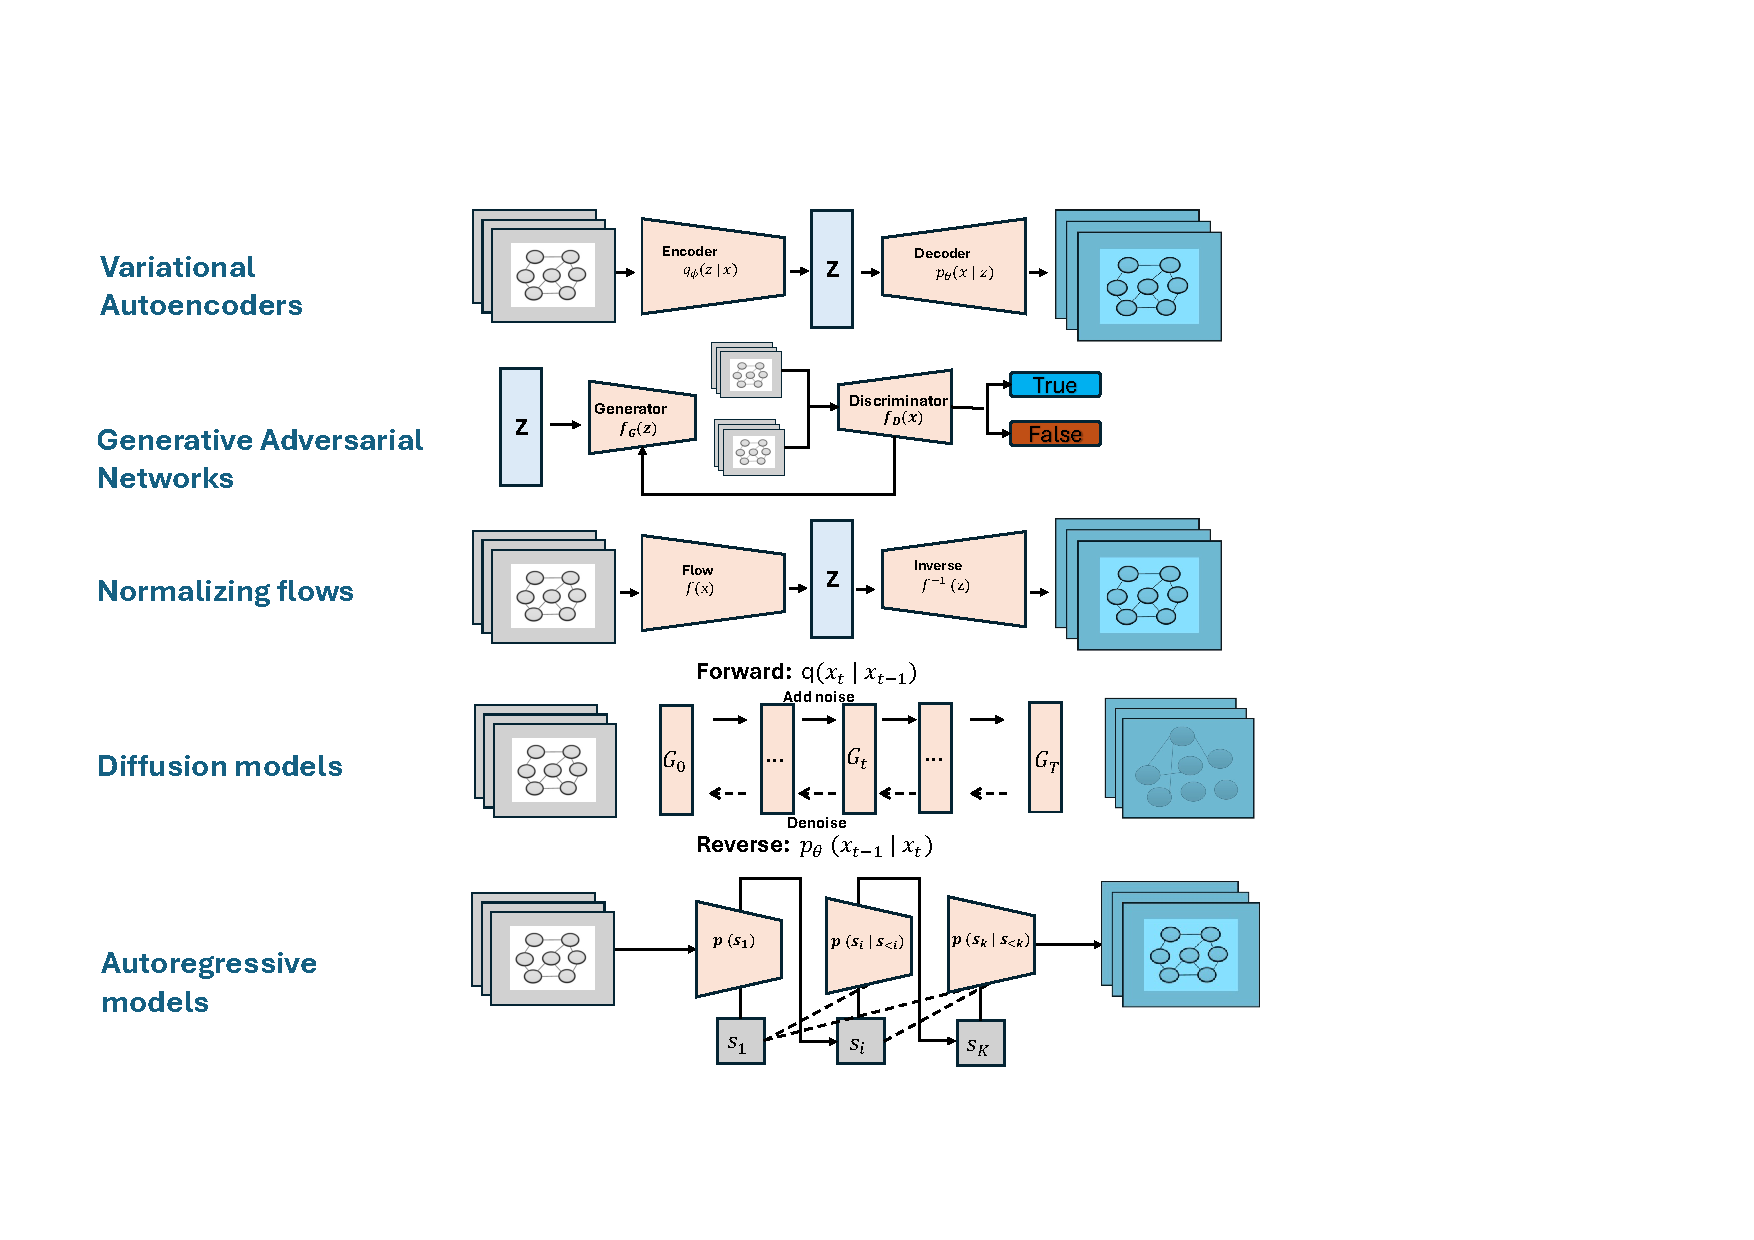
\includegraphics[width=1.5\textwidth]{images/graph_models.pdf}
    \caption{
    Overview of major deep generative modeling paradigms for graphs.
    \textbf{Variational Autoencoders (VAEs)} learn a probabilistic encoder 
    $q_{\phi}(z \mid G)$ and decoder $p_{\theta}(G \mid z)$ to model graph distributions 
    via latent variable inference.
    \textbf{Generative Adversarial Networks (GANs)} train a generator and discriminator 
    in an adversarial min--max game to implicitly approximate the graph data distribution.
    \textbf{Normalizing Flows} construct an invertible mapping between graphs and latent variables, 
    enabling exact likelihood computation via the change-of-variables formula.
    \textbf{Diffusion models} progressively corrupt graphs through a forward noising process 
    and learn a reverse denoising process $p_{\theta}(x_{t-1} \mid x_t)$.
    \textbf{Autoregressive models} factorize the graph likelihood according to the chain rule, 
    generating graph components sequentially as 
    $p(G)=\prod_{i} p(s_i \mid s_{<i})$.
    }
    \label{fig:graph_generative_taxonomy}
\end{figure}
While the preceding discussion focused on how graphs are represented for
downstream predictive tasks, an equally important question concerns how
graphs themselves can be generated. In contrast to representation learning,
graph generation requires modeling the full joint distribution over
combinatorial structures and attributes, posing additional challenges
related to permutation invariance, validity constraints, and scalability.
We therefore now turn to deep generative models for graphs.

\paragraph{Autoregressive Models.}

Autoregressive generative models construct complex data distributions by
factorizing the joint probability of a graph into a product of conditional
distributions using the chain rule of probability.
Given a sequential representation $S = (s_1, \dots, s_K)$ derived from a graph
$G$, the model generates components one step at a time according to
\[
p(G) = \prod_{i=1}^{K} p(s_i \mid s_{<i}),
\]
where $s_{<i}$ denotes the previously generated components.
In the context of graphs, such sequential representations may correspond to
node lists, edge lists, motif sequences, or traversal-based encodings.
Autoregressive approaches therefore generate graphs incrementally, deciding at
each step how to extend the current partial structure.
Representative methods include GraphRNN \citep{graph}, which generates
nodes and their adjacency vectors sequentially, NetGAN \citep{bojchevski2018netgan},
which models random walks as sequences, BiGG \citep{dai2020scalable}, which adopts
a tree-structured edge-generation process, and more recent large language
model–inspired approaches that tokenize graph structures into reversible
sequences \citep{zhao2023graphgpt}.
While autoregressive models provide flexible likelihood-based generation and
naturally handle variable-sized graphs, they often suffer from sequential
sampling inefficiency and sensitivity to the chosen graph ordering.
\paragraph{Variational Autoencoders (VAEs).}
Variational Autoencoders (VAEs) constitute one of the earliest
likelihood-based deep generative modeling paradigms.
They introduce a latent variable model in which observed data
$G$ is generated from a continuous latent representation
$z \sim p(z)$ through a decoder $p_\theta(G \mid z)$.
Because the true posterior $p_\theta(z \mid G)$ is generally intractable,
VAEs employ a variational approximation
$q_\phi(z \mid G)$ and optimize a lower bound on the log-likelihood
via stochastic gradient methods \citep{kingma2013auto,rezende2014stochastic}.
In the context of graph-structured data, VAEs have been adapted
by parameterizing both the encoder and decoder using graph neural
networks. The encoder $q_\phi(z \mid G)$ maps graphs into
continuous latent embeddings, while the decoder $p_\theta(G \mid z)$
reconstructs adjacency structures and node attributes from latent samples.
Representative approaches include the Variational Graph Autoencoder (VGAE)
\citep{kipf2016vgae} and subsequent extensions for structured
graph generation \citep{simonovsky2018graphvae}.

\paragraph{Generative Adversarial Networks (GANs).}

Generative Adversarial Networks (GANs) are implicit generative
models that learn the data distribution through an adversarial
min--max game between two neural networks: a generator
$f_G$ and a discriminator $f_D$.
The generator aims to synthesize graphs that resemble samples
from the true data distribution, while the discriminator seeks
to distinguish generated graphs from real ones.
The adversarial objective can be written as
\[
\min_{f_G} \max_{f_D}
\;
\mathbb{E}_{G \sim p_{\text{data}}}
[\log f_D(G)]
+
\mathbb{E}_{z \sim p(z)}
[\log (1 - f_D(f_G(z)))] ,
\]
where $z$ is drawn from a simple latent prior distribution.

Extending GANs to graph generation introduces additional
challenges due to the discrete and combinatorial nature of
graph structures.
Since gradients cannot be directly propagated through discrete
sampling operations, many graph GAN models rely on
continuous relaxations or reinforcement learning techniques
to enable optimization.
Representative approaches include GraphGAN
\citep{wang2018graphgan}, which models vertex connectivity
via adversarial learning; NetGAN \citep{bojchevski2018netgan},
which generates graphs through biased random walks and
optimizes a Wasserstein adversarial objective; and MolGAN
\citep{de2018molgan}, which integrates adversarial training
with reinforcement learning for molecular graph generation.
Despite their flexibility and ability to produce high-quality
samples, GAN-based graph models often suffer from
training instability, convergence sensitivity, and mode collapse,
which may limit structural diversity and scalability.

\paragraph{Normalizing Flows.}

Normalizing flow models learn an explicit density over data by
composing a sequence of invertible transformations
$f = f_L \circ \dots \circ f_1$ that map graph representations
(e.g., adjacency tensors or edge features) to latent variables
$z$ drawn from a simple base distribution.
Under the change-of-variables formula, the likelihood of a graph
sample $G$ can be computed exactly as
\[
\log p(G)
=
\log p(z)
+
\sum_{\ell=1}^{L}
\log \left| \det
\frac{\partial f_\ell}{\partial h_{\ell-1}}
\right|,
\]
where the determinant of the Jacobian quantifies how each
invertible transformation alters local volume in the data space.
The bijective structure of $f$ enables tractable density estimation
and exact sampling via the inverse mapping $f^{-1}(z)$.In graph generation, early flow-based approaches such as
MoFlow \citep{zang2020moflow}
adopt a two-stage generation procedure in which molecular
bond structures are generated using a Glow-style continuous flow,
followed by conditional generation of atom types.
GraphDF \citep{lu2022graphdf} extends this paradigm by
introducing discrete normalizing flows based on invertible
modulo-shift transformations, thereby avoiding continuous
relaxations and achieving exact invertibility over discrete
graph variables. GGFlow \citep{hou2024improving} combines
discrete flow matching with optimal transport and an
edge-augmented graph transformer to better model complex
bond interactions in molecular graphs. While normalizing flows provide principled density modeling
with exact likelihood evaluation, the requirement of strict
invertibility constrains architectural flexibility and may limit
their ability to capture large-scale, global node–edge
dependencies characteristic of complex graph topology.


\paragraph{Limitations}

Despite substantial advances, existing deep generative models
continue to face fundamental challenges when applied to
graph-structured data.

Likelihood-based approaches such as VAEs require
explicit or implicit handling of permutation invariance.
In practice, this often entails costly graph-matching procedures
or approximate estimation over possible node alignments,
which can significantly increase computational complexity
and introduce approximation bias \citep{simonovsky2018graphvae}.
Adversarial approaches, while capable of producing sharp samples,
are known to suffer from training instability and mode collapse,
potentially limiting the diversity and structural coverage of
generated graphs \citep{de2018molgan}.
Normalizing flow models provide exact likelihood estimation
through invertible transformations; however, the requirement
of bijectivity constrains architectural design and may hinder
their ability to capture complex, large-scale node–edge
dependencies inherent to graph topology \citep{cornish2020relaxing}.

\subsection{Diffusion-Based Generative Models}
\label{sec:theory:diffusion}

Diffusion-based generative models formulate data generation as the reversal of a
gradual stochastic corruption process. Instead of learning a generator in a
single step, these models define a sequence of increasingly noisy latent
variables and learn to invert this process, transforming noise into structured
samples. This paradigm has emerged as a stable and expressive alternative to
adversarial and variational generative models.
Diffusion models can be broadly categorized into three closely related
paradigms: Score Matching with Langevin Dynamics (SMLD),
Denoising Diffusion Probabilistic Models (DDPM),
and continuous-time Score-Based Generative Models (SGMs).
Although differing in formulation, these approaches are mathematically
connected through the estimation of score functions
$\nabla_x \log p_t(x)$ and the reversal of stochastic perturbation processes.

\textbf{Score Matching with Langevin Dynamics} (SMLD)
\citep{song2019generative}
perturbs data using noise at multiple scales and trains a neural
network to approximate the score function of the perturbed
distribution. Samples are generated using annealed Langevin
dynamics, which iteratively refines noise using gradient-based
updates. \textbf{Denoising Diffusion Probabilistic Models} (DDPM)
\citep{ho2020ddpm} instead formulate diffusion as a discrete-time
Markov chain inspired by nonequilibrium thermodynamics,
learning a parameterized reverse process that inverts a fixed
Gaussian noising schedule. \textbf{Stochastic Differential Equations } (Score SDEs)
\citep{song2020score} generalize discrete diffusion processes
to stochastic differential equations (SDEs), modeling the forward
and reverse dynamics in continuous time.
In this formulation, generation corresponds to solving a reverse-time
SDE whose drift term depends on the learned score function.While these paradigms are mathematically connected through score
estimation and time reversal, they differ in how the forward noising process is
defined on graph representations and how discrete structure is recovered during
sampling.

\paragraph{Forward diffusion process.}
Let $x_0 \sim p_{\mathrm{data}} = q(x_0)$ denote a sample from the unknown
data-generating distribution. DDPMs define a fixed forward Markov process
\citep{norris1998markov} that progressively corrupts $x_0$ by injecting Gaussian
noise,
\[
q(x_t \mid x_{t-1}) =
\mathcal{N}\!\left(x_t;\, \sqrt{1-\beta_t}\,x_{t-1},\, \beta_t I\right),
\qquad t=1,\dots,T,
\]
where $\{\beta_t\}_{t=1}^T$ is a predefined noise schedule with $\beta_t\in(0,1)$
and $T \in \mathbb{N}$ denotes the total number of diffusion steps.
As $t$ increases, the distribution of $x_t$ approaches a simple prior, typically
an isotropic Gaussian.
Due to the Markovian structure of the forward process, the marginal distribution
$q(x_t \mid x_0)$ admits a closed form. Defining $\alpha_t = 1-\beta_t$ and
$\bar{\alpha}_t = \prod_{s=1}^t \alpha_s$, we obtain
\[
x_t = \sqrt{\bar{\alpha}_t}\,x_0
      + \sqrt{1-\bar{\alpha}_t}\,\varepsilon,
\qquad \varepsilon \sim \mathcal{N}(0,I),
\]
which allows noisy latent variables to be sampled at arbitrary diffusion times
without simulating the entire chain.

\textbf{Reverse denoising process and learning objective.}
The generative task is to learn a reverse-time Markov chain that inverts the
forward corruption process. DDPMs parameterize the reverse transitions as
\[
p_\theta(x_{t-1} \mid x_t)
=
\mathcal{N}\!\left(x_{t-1};\, \mu_\theta(x_t,t),\, \Sigma_\theta(x_t,t)\right),
\]
where the mean and variance are predicted by a neural network with parameters
$\theta$.
Training is formulated as variational inference: the parameters $\theta$ are
optimized by maximizing a variational lower bound on $\log p_\theta(x_0)$, which
decomposes into Kullback--Leibler terms between the forward noising process and
the learned reverse transitions \citep{ho2020ddpm,kullback1951information}.
Because this objective involves expectations over $q(x_{1:T}\mid x_0)$, it is
estimated using Monte Carlo sampling \citep{robert2004montecarlo} over diffusion
time steps $t$ and Gaussian noise realizations $\varepsilon$.

Ho et al.~\citep{ho2020ddpm} show that, under a suitable parameterization, this
objective reduces to a denoising regression problem in which a neural network
$\varepsilon_\theta$ is trained to predict the injected noise,
\[
\varepsilon_\theta(x_t,t) \approx \varepsilon,
\]
leading to the loss
\[
\mathbb{E}_{t,x_0,\varepsilon}
\bigl[
\|\varepsilon - \varepsilon_\theta(x_t,t)\|^2
\bigr].
\]
This formulation is closely related to denoising score matching
\citep{yang2023diffusion_survey}.
Generation proceeds by sampling $x_T \sim \mathcal{N}(0,I)$ and iteratively
applying the learned reverse transitions until a sample $x_0$ is obtained.
Although exact likelihood evaluation is typically intractable, DDPMs define a
probabilistic generative model and optimize a variational lower bound on the
data likelihood.


\subsubsection{Generative Diffusion Models on Graphs}
\label{sec:related:graph_diffusion_paradigms}

Diffusion and score-based generative models have become a dominant
approach for high-fidelity generation across modalities such as images,
audio, and 3D data \citep{ho2022cascaded,kong2021diffwave,luo2021pointcloud}.
Their appeal lies in stable optimization objectives, strong empirical
sample quality, and flexible conditioning mechanisms.
However, extending diffusion models to \emph{graph-structured} data
introduces additional challenges. Graphs combine discrete combinatorial
structure (edges and categorical types) with continuous attributes
(node features or geometric coordinates), must respect permutation
symmetry, and often require domain-specific validity constraints such as
connectivity, bounded degree, or chemical valency
\citep{jo2022gdss,vignac2022digress}.

Existing approaches can be organized according to how the diffusion
process is instantiated over graph representations.

\textbf{Discrete diffusion over categorical structure.}
For graphs with categorical node and edge variables, several works
adapt DDPM-style diffusion by defining discrete forward Markov
transitions directly over node and edge states.
Rather than adding Gaussian noise, the forward process applies
time-dependent transition matrices to corrupt categorical variables,
and the reverse process is trained as a sequence of classification
problems. DiGress \citep{vignac2022digress} is a representative
example: it diffuses discrete node and edge attributes and employs
a graph Transformer to predict the clean categorical distribution
at each step, trained via cross-entropy losses.
Such discrete formulations preserve combinatorial semantics more
faithfully than continuous relaxations.
In molecular generation, hybrid variants combine discrete diffusion
over atom and bond types with equivariant components for continuous
3D geometry \citep{hoogeboom2022equivariant}, and property-guided
sampling can be incorporated to bias generation toward desired
graph-level characteristics \citep{ho2022classifier}.

\textbf{Continuous diffusion over relaxed graph representations.}
An alternative line of work adopts score-based generative modeling
\citep{song2019generative,song2020score} and defines diffusion in a
continuous space, such as relaxed adjacency matrices, node embeddings,
or geometric coordinates.
A noise-conditional network is trained to estimate the score of
perturbed graph representations, and samples are generated via
Langevin dynamics or related reverse-time procedures.
Early examples include EDP-GNN \citep{niu2020permutation}, which
diffuses relaxed adjacency structure using a permutation-equivariant
GNN, and ConfGF \citep{shi2021learning}, which applies score-based
modeling directly to molecular conformations in continuous coordinate
space.

\textbf{Continuous-time SDE formulations.}
Score-based diffusion can further be generalized to continuous time
using stochastic differential equations (Score SDEs)
\citep{song2020score}. In this framework, graph features evolve
according to coupled stochastic dynamics, and generation corresponds
to solving reverse-time differential equations driven by the learned
score function.
GraphGDP \citep{huang2022graphgdp} and GDSS \citep{jo2022gdss}
define such SDEs over node and edge variables while enforcing
permutation equivariance in the score network.
A recurring challenge in continuous formulations is that isotropic
Gaussian noise rapidly densifies sparse adjacency representations;
spectral or low-rank variants mitigate this by diffusing in
structured subspaces that better preserve informative graph structure
\citep{luo2023fast}.

\textbf{Design trade-offs and structural limitations.}
Across these paradigms, graph diffusion models must make a series
of interdependent design choices:
(i) the representation space over which diffusion is defined
(discrete categories, continuous adjacency relaxations, node/edge
features, latent embeddings, or spectra);
(ii) the enforcement of permutation symmetry (and, in geometric
settings, E(3)-equivariance);
(iii) the modeling of variable graph size; and
(iv) the incorporation of validity constraints.

These choices expose characteristic failure modes.
Continuous relaxations may blur combinatorial structure and require
post-hoc discretization; direct diffusion over adjacency often
destroys sparsity; and unconstrained denoising dynamics do not
naturally enforce global structural constraints such as connectivity
or degree consistency.
Consequently, many approaches rely on architectural inductive bias,
guided sampling, or auxiliary decoding procedures to restore
structural validity.These challenges motivate the diffusion-based graph generator developed in
Chapter~4, which separates continuous denoising from discrete constrained
graph reconstruction.



\section{Evaluation of Graph Generative Models}
\label{sec:related:evaluation}

Evaluating generative models remains a long-standing and unresolved challenge.
Modern generative tasks typically involve high-dimensional data with complex dependencies
between components, for which direct distributional comparison is intractable.
As a result, most evaluation strategies rely on indirect comparisons between real and
generated samples, using either summary statistics, divergence measures, or learned
representations.

In domains such as image generation, visual inspection is a useful diagnostic but an unreliable proxy for generalization or downstream utility\citep{theis2016note} ; evaluation should therefore be aligned with the intended application and
the failure modes of interest. In high-dimensional settings
several commonly used criteria for generative models---including average log-likelihood,
proxy likelihood estimates (e.g., Parzen windows), and \emph{visual sample fidelity}---can be
largely independent. Visually
convincing samples are neither sufficient nor necessary for high likelihood, and that Parzen-window estimates can be unreliable and yield pathological rankings.  

Early and widely adopted approaches reduce evaluation to scalar summary statistics such
as the Inception Score (IS)~\citep{salimans2016improved}, the Fr\'echet Inception Distance
(FID)~\citep{heusel2017gans}, and kernel-based distances including MMD and KID
~\citep{gretton2012kernel,binkowski2018demystifying}. These metrics gained popularity due
to their simplicity and ease of comparison across models. However, their limitations are
now well established: they are sensitive to preprocessing choices and sample size, rest
on strong distributional assumptions, and often correlate weakly with human judgment or
downstream task performance
~\citep{theis2016note,barratt2018note,chong2020effectively,parmar2022aliased,borji2019pros,borji2022pros,betzalel2024evaluation,stein2023exposing}.
Empirical studies further show that model rankings induced by such scores can be unstable
under minor perturbations, while offering limited insight into the causes of model success
or failure. For example, \citet{betzalel2024evaluation} report that IS/FID can be substantially
more volatile than probabilistic divergences in controlled settings, and that the induced \emph{rankings}
of nearby models can vary considerably; they quantify this explicitly using rank-correlation
measures such as Spearman's $\rho$ and Kendall's $\tau$.
A more general statistical approach compares empirical distributions using two-sample
tests such as the \emph{Maximum Mean Discrepancy} (MMD). Given two sample sets
\(X = \{x_i\}_{i=1}^n\) and \(Y = \{y_j\}_{j=1}^m\), MMD is defined as
\[
\mathrm{MMD}(X,Y) =
\frac{1}{n^2}\sum_{i,j=1}^n k(x_i,x_j)
+ \frac{1}{m^2}\sum_{i,j=1}^m k(y_i,y_j)
- \frac{2}{nm}\sum_{i=1}^n\sum_{j=1}^m k(x_i,y_j),
\]
where \(k(\cdot,\cdot)\) is a positive definite kernel defined either directly on structured
objects or on vector-valued representations. A common choice is the radial basis function
kernel
\[
k(x_i, x_j) = \exp\!\left(-\frac{d(x_i, x_j)^2}{2\sigma^2}\right),
\]
where \(d(\cdot,\cdot)\) denotes a distance measure and \(\sigma\) is a bandwidth parameter.
Although MMD is consistent under suitable conditions, it does not necessarily increase
monotonically with distributional dissimilarity, complicating interpretation
~\citep{obrady2021evaluation}. Related divergences, such as average Kullback--Leibler
divergence~\citep{kullback1951information}, are often applied to specific marginal
statistics, but inherit similar limitations.

To address the shortcomings of scalar divergences, a line of work has proposed
multi-dimensional diagnostics that explicitly disentangle \emph{fidelity} and
\emph{diversity}. Examples include precision--recall for distributions
~\citep{sajjadi2018assessing,kynkaanniemi2019improved}, density--coverage
~\citep{naeem2020reliable}, and entropy or spectrum-based measures such as VENDI SCORE and
FKEA~\citep{friedman2023vendi,pasarkar2024cousins,jalali2024fkea,luo2024converge}.
These approaches can expose failure modes such as mode collapse or poor coverage that
scalar scores often obscure. Nevertheless, they remain strongly dependent on the chosen
representation space, can be unstable under embedding shifts, and typically lack
distribution-free guarantees that would ensure reliability across domains
~\citep{parmar2022aliased,betzalel2024evaluation}. More broadly, large-scale empirical studies
suggest that evaluation outcomes can depend strongly on the \emph{feature extractor} used to build
the representation space, and that commonly used encoders may fail to capture perceptually relevant
differences across datasets and model families~\citep{stein2023exposing}.

A complementary perspective evaluates generative models through supervised learning
performance. Classifier-based protocols such as GAN-train/test~\citep{shmelkov2018good}
and train-on-synthetic, test-on-real (TSTR)
~\citep{hyland2017real,esteban2017real,yoon2019timegan} assess whether models trained on
generated data generalize to real test sets. This framing directly links evaluation to
practical utility, treating synthetic data as a substitute or augmentation for real data.
In practice, however, such methods are typically reported as point estimates without
uncertainty quantification and tend to conflate distinct sources of failure—such as
distributional shift, loss of diversity, or overfitting—into a single outcome.



Domain-specific benchmarks provide another perspective on generative model evaluation.
In molecular and graph generation, for instance, frameworks such as \textsc{GuacaMol} and
\textsc{MOSES}~\citep{brown2019guacamol,polykovskiy2020moses} test for validity, uniqueness,
novelty, and agreement with basic property distributions.
These criteria are useful as sanity checks, but remain narrow: a model can satisfy them by
producing near-duplicate samples, and they often fail to assess whether generated data
supports downstream predictive modeling tasks.Motivated by these limitations, recent work has increasingly shifted attention from
\emph{individual metrics} to \emph{evaluation frameworks} that study how conclusions vary
across metrics, datasets, and experimental choices.
Rather than collapsing performance to a single scalar score, these approaches emphasize
multi-objective trade-offs, sensitivity analysis, and the stability of conclusions under
perturbations of the evaluation protocol.
For example, \citet{hall2024evalgim} introduce EvalGIM, a unified benchmarking library for
text-to-image generative models that consolidates metrics of quality, diversity, and
consistency and organizes them into structured ``evaluation exercises.''
EvalGIM highlights trade-offs via Pareto-front analyses and explicitly examines the
\emph{robustness of model rankings} across metrics and datasets, showing that apparent
model superiority can depend strongly on the evaluation choices.
However, frameworks such as EvalGIM remain \emph{domain-specific}, and their conclusions are
tied to particular data modalities, representation spaces, and task assumptions.
More fundamentally, they stop short of providing a \emph{statistically grounded,
domain-agnostic formulation} of generative model evaluation.
Taken together, the existing literature reveals a fragmented evaluation landscape:
scalar heuristics are simple but brittle; multi-dimensional diagnostics provide richer
signals but remain representation-dependent; classifier-based methods link evaluation
to downstream utility but often lack uncertainty quantification and diagnostic separation.
No single metric is sufficient in isolation, and conclusions drawn from individual scores
can be unstable under changes in datasets, metrics, or feature extractors.

These limitations motivate a shift in perspective: rather than treating
evaluation as the optimization of a single numerical score or relying on
representation-dependent heuristics, generative model assessment should be
formulated as a statistically grounded learning problem. In this thesis,
we adopt a classifier-based perspective in which evaluation metrics are
derived from predictive tasks defined on real and generated data.
By interpreting these metrics as empirical risk estimators within the
PAC (Probably Approximately Correct) framework, we obtain explicit uncertainty control and finite-sample
generalization guarantees.
Within this formulation, the central object of interest is not an absolute
score, but the reliability and stability of relative comparisons between
models across datasets and evaluation criteria. Model assessment therefore
naturally reduces to a ranking problem, where conclusions are supported by
statistical guarantees and robustness analyses rather than isolated scalar
values. This learning-theoretic perspective enables evaluation procedures
that are interpretable, resistant to memorization artifacts, and applicable
across data modalities, while explicitly separating distinct failure modes
such as distributional shift, loss of diversity, and predictive inadequacy. These limitations motivate the statistically grounded evaluation framework
developed in Chapter~5, which formulates generative model assessment as a
learning problem with uncertainty-controlled model ranking.

\subsection{Learning-Theoretic Preliminaries for Generative Evaluation}
\label{sec:theory:eval_preliminaries}
We briefly recall standard learning-theoretic concepts that underpin the
classifier-based evaluation framework developed later in this thesis.
Throughout, we consider supervised learning with finite samples and
probabilistic generalization guarantees in the
Probably Approximately Correct (PAC) framework
\citep{vapnik1998statistical}.
These tools allow evaluation procedures based on learned predictors to be
interpreted as statistical estimators with explicit uncertainty control.

Let $\mathcal{X}$ denote an input space and $\mathcal{Y}$ a label space.
A hypothesis class $\mathcal{H}$ consists of functions
$h : \mathcal{X} \to \mathcal{Y}$.
Given a data-generating distribution $P$ over $\mathcal{X}\times\mathcal{Y}$ and
a loss function $\ell : \mathcal{Y}\times\mathcal{Y}\to[0,1]$, the
\emph{population risk} of a hypothesis $h$ is
\[
R_P(h) := \mathbb{E}_{(x,y)\sim P}\bigl[\ell(h(x),y)\bigr].
\]
Given a finite sample $S=\{(x_i,y_i)\}_{i=1}^n$ drawn i.i.d.\ from $P$, the
\emph{empirical risk} is
\[
\widehat R_S(h) := \frac{1}{n}\sum_{i=1}^n \ell(h(x_i),y_i).
\]
An empirical risk minimizer (ERM) is any
\[
\hat h_S \in \arg\min_{h\in\mathcal{H}} \widehat R_S(h).
\]

\paragraph{PAC generalization.}
In the PAC framework, one seeks uniform convergence bounds of the form
\[
\Pr\Big(
\sup_{h\in\mathcal{H}}
\bigl|R_P(h) - \widehat R_S(h)\bigr|
\le \varepsilon(n,\delta,\mathcal{H})
\Big) \ge 1-\delta,
\]
where $\varepsilon$ depends on the sample size $n$, confidence level $\delta$,
and the capacity of the hypothesis class $\mathcal{H}$.
Such bounds justify the use of empirical performance as a proxy for population
performance with high probability.

\paragraph{VC dimension.}
For binary classification, the capacity of a hypothesis class $\mathcal{H}$ can
be characterized by its Vapnik--Chervonenkis (VC) dimension
\citep{vapnik1998statistical}.
A set $\{x_1,\dots,x_m\}\subset\mathcal{X}$ is said to be \emph{shattered} by
$\mathcal{H}$ if $\mathcal{H}$ realizes all $2^m$ binary labelings on that set.
If $\mathcal{H}$ has finite VC dimension $d$, then with probability at least
$1-\delta$,
\[
\sup_{h\in\mathcal{H}}
\bigl|R_P(h)-\widehat R_S(h)\bigr|
\;\le\;
O\!\left(
\sqrt{\frac{d\log(n/d)+\log(1/\delta)}{n}}
\right),
\]
for $0$--$1$ loss.

\paragraph{Rademacher complexity.}
For real-valued hypothesis classes, tighter and more general bounds can be
obtained using Rademacher complexity
\citep{bartlett2002rademacher}.
Given a sample $S=\{x_i\}_{i=1}^n$, the empirical Rademacher complexity of
$\mathcal{H}$ is
\[
\mathfrak{R}_S(\mathcal{H})
:=
\mathbb{E}_{\sigma}
\left[
\sup_{h\in\mathcal{H}}
\frac{1}{n}\sum_{i=1}^n \sigma_i h(x_i)
\right],
\]
where $\sigma_i$ are i.i.d.\ Rademacher variables taking values in $\{-1,+1\}$.
If the class is real-valued (e.g.\ $\mathcal{H}\subseteq\{h:\mathcal{X}\to[0,1]\}$,
or we apply the bound to the loss class $\ell\circ\mathcal{H}$),
then with probability at least $1-\delta$,
\[
\sup_{h\in\mathcal{H}}
\bigl|R_P(h)-\widehat R_S(h)\bigr|
\;\le\;
2\mathfrak{R}_S(\mathcal{H})
+ O\!\left(\sqrt{\frac{\log(1/\delta)}{n}}\right).
\]

\paragraph{Concentration inequalities.}
Many evaluation metrics reduce to averages of bounded random variables.
Hoeffding’s inequality \citep{hoeffding1963probability} states that if
$X_1,\dots,X_n$ are independent with $X_i\in[0,1]$ and mean $\mu$, then for any
$\varepsilon>0$,
\[
\Pr\bigl(|\tfrac{1}{n}\sum_{i=1}^n X_i - \mu| > \varepsilon\bigr)
\le 2\exp(-2n\varepsilon^2).
\]
Joint guarantees across multiple models, metrics, or resampling splits are
obtained using the union bound.

\paragraph{Domain adaptation and discrepancy.}
Classifier-based generative evaluation often compares predictors trained or
tested on samples drawn from different distributions.
Let $P$ and $Q$ be distributions over $\mathcal{X}$.
For a hypothesis class $\mathcal{H}$, the
$\mathcal{H}\Delta\mathcal{H}$ discrepancy is defined as
\[
\mathrm{disc}_{\mathcal{H}\Delta\mathcal{H}}(P,Q)
:=
2 \sup_{h,h'\in\mathcal{H}}
\bigl|
\Pr_{x\sim P}[h(x)\neq h'(x)]
-
\Pr_{x\sim Q}[h(x)\neq h'(x)]
\bigr|.
\]
Define the joint optimal risk
\[
\lambda(P,Q) := \min_{h\in\mathcal{H}}
\bigl(R_P(h) + R_Q(h)\bigr).
\]
Following \citet{ben2010theory}, for any $h\in\mathcal{H}$,
\[
|R_P(h)-R_Q(h)|
\le \tfrac{1}{2}\mathrm{disc}_{\mathcal{H}\Delta\mathcal{H}}(P,Q) + \lambda(P,Q).
\]
This inequality formalizes how distributional shift between real and generated
data affects predictive performance.

\paragraph{Lipschitz functions and entropy.}
A function $f:\mathbb{R}\to\mathbb{R}$ is $L$-Lipschitz if
$|f(a)-f(b)|\le L|a-b|$ for all $a,b$.
The binary entropy function
\[
H(p) := -p\log p - (1-p)\log(1-p)
\]
is Lipschitz on any interval $[\tau,1-\tau]$ with $\tau>0$
\citep{cover2006elements}.
This property allows concentration bounds on neighbourhood proportions to be
transferred to entropy-based similarity measures used later in this thesis.
\paragraph{}
These learning-theoretic tools will be used in Chapter~\ref{ch:rankgen}
to derive generalization guarantees for classifier-based evaluation metrics,
including normalized Train-on-Synthetic-Test-on-Real (TSTR) performance ratios.
\section{Chapter conclusions}
\label{sec:related:conclusions}

This chapter established the theoretical foundations required for the
methodological developments presented in the remainder of the thesis. We first
introduced graphs as structured objects with discrete topology and optional
node and edge attributes, together with the matrix representations,
neighbourhood structures, and permutation symmetries that govern learning on
graph-structured data.

We then reviewed the principal approaches to graph representation learning.
Predefined representations, including structural descriptors and graph
kernels, provide deterministic and often interpretable mappings based on
well-defined graph substructures. Learned representations, including
random-walk embeddings, graph neural networks, and graph Transformers, instead
optimise parameterised mappings from data and can adapt their representations
to a particular task. The review highlighted an important trade-off between
the interpretability and reproducibility of explicit representations and the
flexibility of learned models, particularly for graphs with continuous
attributes.

The chapter subsequently examined deep generative modelling for graphs. Unlike
generation in regular Euclidean domains, graph generation must account for
permutation symmetry, variable graph sizes, discrete and sparse topology, and
global validity constraints. Diffusion-based methods provide a flexible
framework for generative modelling, but their application to graphs requires
careful choices regarding the representation being diffused and the recovery
of valid discrete structure.

Finally, we reviewed existing approaches to generative-model evaluation,
ranging from scalar distributional measures and multi-dimensional diagnostics
to class\-ifier-based protocols. This discussion showed that evaluation outcomes
can depend strongly on the selected representation, metric, and experimental
protocol, and that point estimates alone provide limited information about the
reliability of model comparisons. The learning-theoretic concepts introduced
in this chapter provide the basis for treating classifier-based evaluation as
a statistical estimation problem with explicit finite-sample uncertainty.

These foundations motivate the three methodological contributions developed in
the following chapters. Chapter~\ref{ch:nsppk} introduces an explicit
kernel-based representation for attributed graphs.
Chapter~\ref{ch:generator} develops a conditional graph-generation framework,
and Chapter~\ref{ch:rankgen} presents a statistically grounded framework for
evaluating and ranking generative models.

\chapter{Interpretable Graph Representations with NSPPK}
\label{ch:nsppk}


\section{Introduction}

Chapter~\ref{ch:theory} established the theoretical foundations of graph
representation learning and highlighted the complementary strengths of
predefined kernel methods and learned neural embeddings.
In particular, kernel-based representations offer deterministic feature
construction, transparent feature maps, and favourable behaviour in low-data
regimes, while neural approaches provide greater expressive flexibility at the
cost of increased training complexity and reduced transparency.

A key limitation identified in Chapter~\ref{ch:theory} concerns the treatment of
\emph{continuous node attributes} within scalable graph kernel frameworks.
Many classical kernels were originally designed for discretely labelled graphs
and rely on exact substructure matching. When applied to graphs with
real-valued features, these methods typically require discretisation or
hashing procedures that introduce artificial thresholds, reduce numerical
fidelity, and may distort similarity relationships. Although several extensions
incorporate continuous attributes through embeddings or propagation
mechanisms, they often sacrifice either scalability, robustness, or explicit
feature interpretability.

This chapter addresses this limitation by developing an explicit graph kernel
that integrates continuous node attributes directly into the feature
construction process while retaining the computational efficiency and
interpretability of classical substructure-based methods.

\paragraph{Chapter contribution.}
We introduce the \emph{Neighborhood Subgraph Pairwise Path Kernel} (NSPPK),
an explicit graph kernel that extends the
\emph{Neighborhood Subgraph Pairwise Distance Kernel}
(NSPDK)~\citep{costa2010fast}. While NSPDK compares fixed-radius neighbourhoods
around pairs of nodes, NSPPK enriches this representation to capture more
informative structural dependencies and to operate directly on real-valued node
features.

NSPPK advances prior work in three principal ways. First, it replaces
comparisons based solely on fixed-radius neighbourhoods with features derived
from unions of shortest-path neighbourhoods between node pairs, allowing the
representation to capture longer-range structural interactions. Second,
continuous node attributes are incorporated directly into the feature
construction without discretisation, preserving fine-grained information that
would otherwise be lost. Third, NSPPK produces explicit and sparse graph-level
embeddings, enabling kernel evaluation through efficient dot-product
computation. Under fixed parameters, feature extraction scales near-linearly
with graph size and the overall procedure is naturally parallelisable.

The empirical sections test whether this explicit construction can remain
accurate, scalable, and interpretable on attributed graph benchmarks. The
analysis focuses on predictive performance, runtime behaviour, feature
inspection, robustness to perturbations, and larger citation-network case
studies.

The remainder of this chapter is organised as follows.
Section~\ref{sec:relatedwork} reviews the graph-kernel literature most closely
related to NSPPK.
Section~\ref{sec:notation} introduces the NSPPK-specific notation and core
objects.
Section~\ref{sec:method} presents the feature construction and hashing scheme.
Section~\ref{sec:complexity} analyses computational complexity.
Section~\ref{sec:Diagonal} reports a controlled robustness analysis.
Section~\ref{sec:experiments} reports empirical results.
Section~\ref{sec:nsppk:discussion-limitations} discusses limitations.
Section~\ref{sec:Conclusion} concludes the chapter.

\section{Related Work}
\label{sec:relatedwork}

Chapter~\ref{ch:theory} situated graph kernels within the broader landscape of
graph representation learning, distinguishing explicit, predefined
representations from learned neural embeddings, and highlighted the particular
difficulty of handling continuous node attributes in scalable and interpretable
kernel frameworks. In this chapter, we therefore focus on the graph-kernel
literature most directly related to NSPPK.

Many graph kernels are formulated within the \emph{R-convolution} framework

\citep{haussler1999}, which defines similarities between structured objects by
decomposing them into collections of substructures and aggregating comparisons
over these parts. Within this family, the most direct predecessor of NSPPK is
the Neighborhood Subgraph Pairwise Distance Kernel (NSPDK)
\citep{costa2010fast}, which compares pairs of rooted neighbourhoods at fixed
graph distances. NSPDK is scalable and interpretable, but it was originally
designed for discrete labels and represents interactions between anchors only
through local neighbourhoods and their pairwise distance.

Several graph kernels have been proposed to extend this paradigm to continuous
node attributes. Propagation kernels \citep{neumann2016propagation} achieve
near-linear runtime by diffusing and hashing node attributes, but rely on
discretisation and may lose fine-grained numerical information. GraphHopper
\citep{feragen2013scalable} extends shortest-path kernels to attributed graphs
through node kernels evaluated along shortest paths, but remains
computationally more expensive and does not yield sparse explicit graph-level
feature maps. Wasserstein Weisfeiler--Lehman
\citep{togninalli2019wasserstein} replaces exact substructure matching with
optimal transport between distributions of refined node embeddings, increasing
flexibility at the cost of dense representations and higher computational
overhead.

More recent approaches such as MMD-GK \citep{mmdgk_iclr2024}, SWWL
\citep{carpintero2024swwl}, and DSP \citep{ye2025dsp} further shift away from
explicit combinatorial substructures by representing graphs as distributions of
node-, subgraph-, or path-level embeddings. These methods avoid strict discrete
matching, but typically rely on dense similarity computations, distribution
matching, or learned substructure representations, which can reduce
interpretability and increase memory and runtime requirements.

As discussed in Chapter~\ref{ch:theory}, graph neural networks provide an
alternative route for handling continuous attributes, since they learn
representations directly from graph structure and features. However, they are
training-based, task-dependent, and generally less interpretable than explicit
kernel features. In this chapter, they therefore serve primarily as empirical
baselines rather than direct methodological predecessors.

In contrast, NSPPK remains firmly within the explicit substructure-kernel para
digm. It extends NSPDK by enriching anchor-pair comparisons with unions of
shortest paths and by integrating continuous node attributes directly into the
explicit feature construction, without discretisation. In doing so, it aims to
occupy the methodological space identified in Chapter~\ref{ch:theory}: an
interpretable, deterministic, and scalable graph representation that retains
the advantages of explicit kernels while better supporting attributed graphs.





\section{Method}
\label{sec:method}

  A common strategy for defining kernels over structured objects is to decompose
them into collections of \emph{substructures} and compare these using a base
kernel. Kernels of this form fall under the \emph{R-convolution}
framework~\citep{haussler1999}, which subsumes many classical graph kernels.

A representative example is the Neighborhood Subgraph Pairwise Distance Kernel
(NSPDK)~\citep{costa2010fast}, which compares pairs of rooted neighbourhoods
whose centers lie at a prescribed graph distance. NSPDK yields explicit sparse
feature maps through permutation-invariant hashing, making feature extraction
efficient and kernel evaluation reducible to a sparse dot product.

Despite these strengths, NSPDK has two important limitations in the present
setting. First, it relies on exact matching of discrete node labels and thus
does not directly support real-valued node attributes. Second, its structural
features are defined only through pairs of fixed-radius neighbourhoods and their
distance. In graphs with high-degree nodes or multiple alternative routes
between anchors, this representation can become overly instance-specific:
similar neighbourhoods may fail to recur across graphs, feature overlap becomes
sparse, and the Gram matrix may become diagonally dominant, reducing
statistical coupling between training instances.

To address these limitations, we introduce the
\emph{Neighborhood Subgraph Pairwise Path Kernel} (NSPPK). NSPPK retains the
explicit and hash-based construction of NSPDK, but augments it in two
directions. Structurally, it enriches anchor-pair features with a connector
subgraph defined by the union of all shortest paths between the anchors,
thereby encoding more than distance alone. Attribute-wise, it integrates
continuous node attributes directly into the explicit feature construction,
avoiding discretisation while preserving fine-grained information in a
deterministic and interpretable representation.

\subsection{Core objects and notation}
\label{sec:notation}

We adopt the graph-theoretic notation introduced in
Chapter~\ref{ch:theory}, including shortest-path distance, induced subgraphs,
and $r$-hop neighbourhoods. Here we define only the additional objects that are
specific to NSPPK.

\textbf{Anchor pairs.}
We consider unordered anchor pairs $\{u,v\}\subseteq V$ such that $u$ and $v$
belong to the same connected component and have finite shortest-path distance
$d(u,v)\leq D$. Disconnected pairs are ignored.


\textbf{Union of shortest paths.}
For two vertices $u,v\in V$ with finite shortest-path distance, let $U(u,v)$
denote the subgraph induced by the union of all shortest $u$--$v$ paths.
Thus, $U(u,v)$ contains exactly the vertices and edges that belong to at least
one shortest path between $u$ and $v$.

\textbf{Connector subgraph.}
For a vertex set $S\subseteq V$, let $N_{r'}(S)$ denote the induced subgraph on
all vertices within shortest-path distance at most $r'$ from $S$, namely
\[
N_{r'}(S)
=
G\!\left[\{x\in V : \min_{s\in S} d(x,s)\le r'\}\right].
\]
For a connector radius $r'\ge 0$, we define the connector subgraph
\[
C_{r'}(u,v)
=
N_{r'}\!\big(U(u,v)\big).
\]
Thus, $C_0(u,v)=U(u,v)$, while $r'>0$ thickens the connector by including all
vertices within $r'$ hops of the path-union subgraph.

\textbf{NSPPK feature primitives.}
An NSPPK feature is defined by a pair of anchor neighbourhoods
\[
\bigl(N_{r_u}(u),\,N_{r_v}(v)\bigr),
\]
whose centers are at shortest-path distance $d(u,v)$, optionally augmented with
a connector subgraph $C_{r'}(u,v)$. Each feature is therefore parameterised by
a tuple $(r_u,r_v,d,r')$ and is invariant to permutations of vertices within
the constituent subgraphs.

\subsection{Augmented structural features}

NSPPK extends the feature family of NSPDK by augmenting pairs of rooted
neighbourhoods with an explicit connector subgraph
$C_{r'}(u,v)=N_{r'}(U(u,v))$. Whereas NSPDK represents the interaction between
two anchors only through the distance between them, NSPPK additionally encodes
the structure of the region connecting them.This idea is illustrated in Figure~\ref{fig:example}, which shows how NSPPK
augments two anchor neighbourhoods with a connector subgraph derived from the
union of shortest paths between them.This design is motivated by the observation that, although the number of
distinct shortest paths between two nodes may grow rapidly in graphs with many
cycles or alternative routes, their \emph{union} is uniquely defined as a
single subgraph. This yields a deterministic connector representation that
avoids combinatorial explosion while still capturing the multiplicity and
arrangement of shortest-path alternatives. As shown in Figure~\ref{fig:example}, two anchor pairs may have the same local
neighbourhood radii and the same anchor distance, yet differ in the internal
structure of the connector.

The NSPPK feature family is obtained by enumerating all parameter
configurations
\[
r_u,r_v \in \{0,\ldots,R\},\qquad
d \in \{0,\ldots,D\},\qquad
r' \in \{0,\ldots,R'\}\cup\{\varnothing\},
\]
where $R$, $D$, and $R'$ are small positive integers chosen for tractability.
The special value $r'=\varnothing$ denotes the case in which no connector is
included, recovering a neighbourhood-pair feature analogous to NSPDK.
Figure~\ref{fig:nspdk-vs-nsppk-example} provides a concrete comparison between
the two constructions, showing that the connector allows NSPPK to distinguish
cases that collapse to the same NSPDK feature.
\begin{figure}[t]
  \centering
  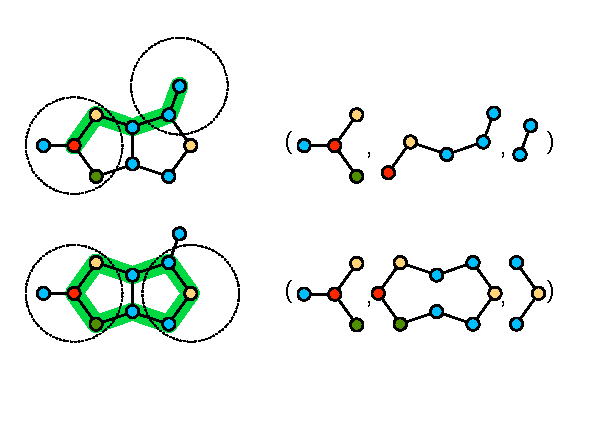
\includegraphics[width=0.65\textwidth]{images/nsppk_features.pdf}
    \caption{Example NSPPK structural features. Top: two radius-1 neighbourhoods
    centred at an anchor pair whose vertices are at shortest-path distance 4,
    together with their union-of-shortest-paths connector for $r'=0$, corresponding
    to a single shortest path. Bottom: an analogous anchor-pair configuration in
    which the two anchors are again at distance 4, but the connector contains two
    distinct shortest paths of length 4.}
  \label{fig:example}
\end{figure}

\subsection{From subgraphs to explicit features}

Rather than defining similarity directly between graphs, NSPPK first enumerates
a family of local subgraph patterns. Each pattern is determined by a pair of
anchor neighbourhoods at given radii, together with an optional connector
subgraph derived from the union of shortest paths between the anchors. Every
such configuration is then mapped, through permutation-invariant hashing, to a
feature identifier. A graph is finally represented by a sparse histogram
counting how often each feature occurs.

Formally, let $\theta=(R,D,R')$ denote the maximal radii and distances used in
feature extraction. For a graph $G$, let $f_G^\theta$ denote the vector of NSPPK
feature counts. The kernel between two graphs $G$ and $G'$ is defined as
\[
k_\theta(G,G')
=
{f_G^\theta}^{\top} f_{G'}^\theta.
\]

Because NSPPK features are extracted from unordered anchor pairs, the
graph-level feature vector decomposes as
\[
f_G^\theta
=
\sum_{\substack{\{u,v\}\subseteq V\\u\neq v,\ d(u,v)\le D}}
f_{G,u,v}^\theta,
\]
where $f_{G,u,v}^\theta$ denotes the contribution associated with anchor pair
$\{u,v\}$.

\subsection{Feature hashing pipeline}

To obtain an explicit sparse representation, each structural pattern is mapped
to a hash bucket. Let $b$ denote the number of hash bits. The hash codomain therefore has size
\[
M = 2^b.
\]
Using hashed identifiers allows constant-time indexing into the feature vector
and avoids explicit subgraph isomorphism checks.

A practical advantage of NSPPK is that hashes can be computed
\emph{incrementally} with respect to neighbourhood radius and shortest-path
distance, and cached for reuse. In particular, rooted neighbourhood hashes are
computed once per node and reused when forming neighbourhood-pair and connector
features, avoiding repeated recomputation over anchor pairs.

\textbf{Base hash functions.}
We use SHA-256 as a deterministic hashing function. For any object $x$, let
$\mathrm{sha256}(x)$ denote the integer obtained by applying SHA-256 to a
canonical serialisation of $x$. We define the corresponding $b$-bit base hash as
\[
H_b(x)=\mathrm{sha256}(x)\bmod 2^b.
\]
From $H_b$, we derive two composite operators. First, $H^q(I)$ denotes the
\emph{sequence hash} of an ordered tuple $I=(x_1,\dots,x_k)$, and therefore
preserves the order of its elements. Second, $H^t(S)$ denotes the
\emph{multiset hash} of a multiset $S$; it is computed after lexicographic
sorting and is therefore invariant to permutations of the elements. These two
operators allow NSPPK to distinguish between ordered structural compositions
when order is meaningful, while remaining permutation-invariant for unordered
collections such as neighbourhood shells.

\textbf{Node hash.}
For each node $v$, define the incident-neighbour multiset hash
\[
N_h(v)
=
H^t\!\left(
\{\!\!\{
H^q\big([H_b(\ell(u)), H_b(\ell(e_{v,u}))]\big)
:
u \in N(v)
\}\!\!\}
\right),
\]
and define the rooted node hash as
\[
N_H(v)
=
H^q\big([H_b(\ell(v)), N_h(v)]\big).
\]
When edge labels are unavailable, $\ell(e_{v,u})$ is replaced by a fixed dummy
label.

\textbf{Rooted neighbourhood hash.}
For a node $v$ and shell index $j\ge 0$, let
\[
D_j^v=\{\,u\in V : d(v,u)=j\,\}
\]
be the set of nodes at exact distance $j$ from $v$. Define the shell hash
\[
B_j^v
=
H^t\bigl(\{\!\!\{\,N_H(u) : u\in D_j^v\,\}\!\!\}\bigr),
\]
and then the rooted neighbourhood hash of radius $r$ by
\[
G_H^r(v)
=
H^q([B_0^v,B_1^v,\dots,B_r^v]).
\]
These hashes are computed incrementally in $r$ and cached for each node.

\textbf{Neighbourhood-pair hash.}
For an anchor pair $(u,v)$ at distance $d=d(u,v)$, define
\[
P_H^{r_u,r_v,d}(u,v)
=
H^q\!\left(
\left[
H_b(d),
H^t\!\left(
\left\{\!\!\left\{
H^q([H_b(r_u),G_H^{r_u}(u)]),
H^q([H_b(r_v),G_H^{r_v}(v)])
\right\}\!\!\right\}
\right)
\right]
\right).
\]

\textbf{Connector hash.}
To encode the connector deterministically, we organise its nodes into distance
shells from one anchor node $u$ along the path-union subgraph. Let $U(u,v)$ be
the union of all shortest $u\leftrightarrow v$ paths. We use the notation
$\overline{B}_{j,r'}(u,v)$ to denote a \emph{connector shell hash}, analogous to
the neighbourhood shell hash $B_j^v$ but restricted to nodes lying in the
connector subgraph and constructed from rooted neighbourhood hashes
$G_H^{r'}(\cdot)$ rather than node hashes $N_H(\cdot)$. For each shell index
$j\in\{0,\dots,d(u,v)\}$, define
\[
\overline{B}_{j,r'}(u,v)
=
H^t\bigl(
\{\!\!\{\,G_H^{r'}(w) : w\in D_j^{\,u}\cap V(U(u,v))\,\}\!\!\}
\bigr),
\]
where $V(U(u,v))$ is the vertex set of the path-union subgraph. The connector
hash is then
\[
U_H^{r',d}(u,v)
=
H^q\!\left(
[\overline{B}_{0,r'}(u,v),\dots,\overline{B}_{d,r'}(u,v)]
\right).
\]

\textbf{Final structural feature vector.}
The structural NSPPK vector is obtained by accumulating the hash values of all
neighbourhood-pair and connector features extracted from the graph. The
practical effect of including the connector is illustrated in
Figure~\ref{fig:nspdk-vs-nsppk-example}. Two graphs that are indistinguishable
to NSPDK because they share the same anchor neighbourhoods and anchor distance
are separated by NSPPK once the connector structure is incorporated.

\begin{figure*}[h]
  \centering
  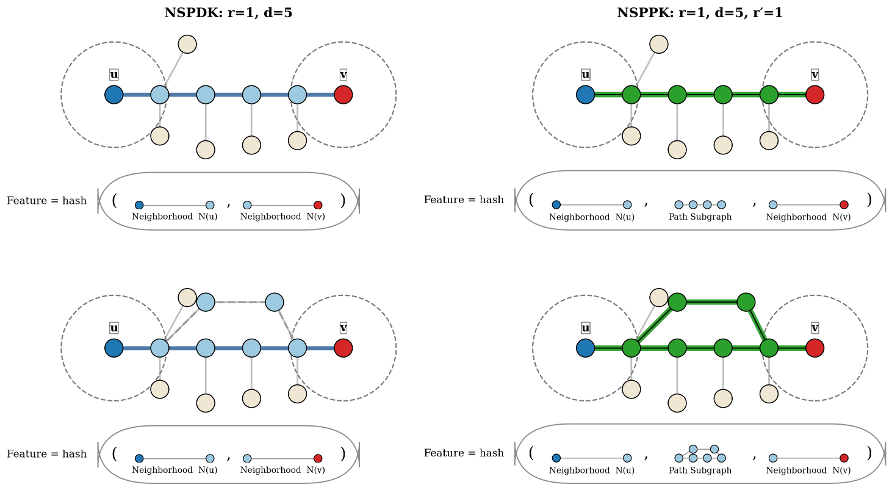
\includegraphics[width=0.95\textwidth]{images/nspdk_vs_nsppk_networkx.png}
  \caption{\textbf{NSPDK vs.\ NSPPK on anchors $u,v$ with $r=1$ and $d=5$.}
  \emph{Left:} NSPDK features for the case with a single shortest path (top) and
  two equal-length shortest paths (bottom). Because NSPDK uses only
  $(N_r(u),d(u,v),N_r(v))$, both cases produce the same feature.
  \emph{Right:} NSPPK includes the connector
  $C_{r'}(u,v)=N_{r'}(U(u,v))$ (shown in green). The connector is a simple path
  in the top graph but a two-path union in the bottom graph, so NSPPK induces
  different features.}
  \label{fig:nspdk-vs-nsppk-example}
\end{figure*}

\subsection{Node attribute integration}
\label{subsec:attribute_integration}

We now extend the structural feature map to graphs with continuous node
attributes. Let
\[
X\in\mathbb{R}^{n\times p}
\]
denote the node-attribute matrix, where each row corresponds to a node and each
column to one of the $p$ attributes. Let
\[
F\in\mathbb{R}^{n\times M}
\]
denote the binary node--feature incidence matrix, where $M=2^b$ is the number of hash buckets and $F_{ij}=1$ if node $i$ contributes to structural feature
$j$. We then define the attribute-augmented representation by
\[
x = \mathrm{vec}(X^\top F)\in\mathbb{R}^{pM}.
\]

In this construction, each structural bucket stores the aggregated continuous
attributes of the nodes contributing to that feature. Thus, structural identity
and continuous attributes are combined within a single explicit feature map.
Node weights can be incorporated by replacing $X$ with $\mathrm{diag}(w)X$,
where $w\in\mathbb{R}^n$ is a vector of node weights. The same mechanism
extends naturally to edge attributes. NSPPK feature extraction remains entirely
deterministic and training-free; supervised learning is introduced only by the
downstream classifier applied to the resulting explicit graph representation.

\subsection{Expressivity Relative to NSPDK and Local Aggregation}
\label{sec:isomorphism}

Distinguishing non-isomorphic graphs is a key requirement for expressive graph
kernels. Two graphs $G=(V_G,E_G)$ and $H=(V_H,E_H)$ are \emph{isomorphic},
denoted $G\cong H$, if there exists a bijection $\pi:V_G\to V_H$ that
preserves adjacency. A valid graph kernel should at least be
\emph{isomorphism-invariant}, meaning that its value does not depend on vertex
ordering. More strongly, one seeks \emph{isomorphism-discrimination}, namely the
ability to assign different similarities to non-isomorphic graphs whenever
their structural differences are visible to the feature map.

The expressive power of many classical graph kernels and message-passing graph
neural networks is closely tied to the
\emph{1-dimensional Weisfeiler--Lehman (1-WL)} test
\citep{shervashidze2011weisfeiler,morris2019weisfeiler}. In particular,
graphs that are indistinguishable by 1-WL cannot be separated by WL-based
kernels, and standard message-passing GNNs are likewise bounded by 1-WL in
distinguishing power \citep{xu2019powerful}. Although higher-order WL variants
can increase expressivity, they generally do so at substantially higher
computational cost.

NSPPK complements local aggregation by encoding not only rooted neighbourhoods
around anchor nodes, but also the connector structure between them. Its
features have the form
\[
\psi\bigl(N_{r_u}(u),\,C_{r'}(u,v),\,N_{r_v}(v)\bigr),
\]
where $\psi(\cdot)$ denotes the NSPPK feature identifier associated with the
anchor neighbourhoods and connector, and
$C_{r'}(u,v)=N_{r'}(U(u,v))$ is derived from the union of all shortest paths
between the anchors. Consequently, two graphs may share identical local anchor
neighbourhoods and the same anchor distance, yet still be separated by NSPPK iif the connector encodings produced by NSPPK differ.

Figure~\ref{fig:isomorphism} illustrates graph pairs that standard local
aggregation schemes fail to distinguish reliably from neighbourhood information
alone. NSPPK can separate such pairs by explicitly encoding the shortest-path
connectivity pattern between anchors rather than relying only on local rooted
structure.
% ---- Figure 1 ----
\begin{figure}[H]
\centering
\begin{adjustbox}{max width=\linewidth}
\begin{tikzpicture}[x=1cm,y=1cm, line cap=round, line join=round,
                    every node/.style={outer sep=0pt}]

  \tikzset{
    panel/.style={rounded corners=2mm, draw=black!20, fill=black!2, line width=0.4pt},
    edge/.style={line width=0.95pt, draw=black!70},
    vblue/.style={circle, draw=blue!55!black, fill=blue!40, minimum size=6.2pt, inner sep=0pt},
    vgreen/.style={circle, draw=teal!55!black, fill=teal!40, minimum size=6.2pt, inner sep=0pt},
    vred/.style={circle, draw=red!55!black, fill=red!40, minimum size=6.2pt, inner sep=0pt},
    vyellow/.style={circle, draw=orange!55!black, fill=orange!40, minimum size=6.2pt, inner sep=0pt}
  }

  \node[panel, minimum width=7.6cm, minimum height=3.6cm, anchor=center] (A) at (0,0) {};
  \node[panel, minimum width=7.6cm, minimum height=3.6cm, anchor=center] (B) at (8.8,0) {};
  \node[anchor=west] at ([xshift=-3.6cm,yshift=1.55cm]A.center) {\small\textbf{(a)}};
  \node[anchor=west] at ([xshift=-3.6cm,yshift=1.55cm]B.center) {\small\textbf{(b)}};

  \path[use as bounding box]
    ([xshift=-1mm,yshift=-1mm]A.south west)
      rectangle
    ([xshift=+1mm,yshift=+1mm]B.north east);

  % Panel (a)
  \begin{scope}
    \clip[rounded corners=2mm] (A.south west) rectangle (A.north east);

    \def\R{1.15}
    \foreach \i in {0,...,5} \coordinate (h\i) at ($([xshift=-2.2cm]A.center) + (\i*60:\R)$);
    \foreach \i/\j in {0/1,1/2,2/3,3/4,4/5,5/0} \draw[edge] (h\i)--(h\j);
    \foreach \i in {0,...,5} \node[vblue] at (h\i) {};

    \coordinate (S) at ($([xshift=+2.1cm]A.center)$);
    \coordinate (u1) at ($(S)+(-1.15,  0.55)$);
    \coordinate (u2) at ($(S)+(-0.45,  0.55)$);
    \coordinate (u3) at ($(S)+(-0.80, -0.40)$);
    \coordinate (v1) at ($(S)+( 0.45, -0.55)$);
    \coordinate (v2) at ($(S)+( 1.15, -0.55)$);
    \coordinate (v3) at ($(S)+( 0.80,  0.40)$);
    \foreach \a/\b in {u1/u2,u2/u3,u3/u1,v1/v2,v2/v3,v3/v1} \draw[edge] (\a)--(\b);
    \foreach \p in {u1,u2,u3,v1,v2,v3} \node[vgreen] at (\p) {};
  \end{scope}

  % Panel (b)
  \begin{scope}
    \clip[rounded corners=2mm] (B.south west) rectangle (B.north east);
    \coordinate (c)  at ($([xshift=-2.2cm]B.center)+(0,0)$);
    \coordinate (l1) at ($([xshift=-2.2cm]B.center)+(-0.9, 0.7)$);
    \coordinate (l2) at ($([xshift=-2.2cm]B.center)+(-1.2,-0.6)$);
    \coordinate (r1) at ($([xshift=-2.2cm]B.center)+( 0.9, 0.7)$);
    \coordinate (r2) at ($([xshift=-2.2cm]B.center)+( 1.2,-0.6)$);
    \foreach \a/\b in {l1/c,c/l2,l2/l1,r1/c,c/r2,r2/r1} \draw[edge] (\a)--(\b);
    \foreach \p in {l1,l2,c,r1,r2} \node[vred] at (\p) {};

    \coordinate (g00) at ($([xshift=+2.0cm]B.center)+(-1.2, 0.6)$);
    \coordinate (g01) at ($([xshift=+2.0cm]B.center)+(-1.2,-0.6)$);
    \coordinate (g10) at ($([xshift=+2.0cm]B.center)+( 0.0, 0.6)$);
    \coordinate (g11) at ($([xshift=+2.0cm]B.center)+( 0.0,-0.6)$);
    \coordinate (g20) at ($([xshift=+2.0cm]B.center)+( 1.2, 0.6)$);
    \coordinate (g21) at ($([xshift=+2.0cm]B.center)+( 1.2,-0.6)$);
    \foreach \a/\b in {g00/g10,g10/g20,g01/g11,g11/g21} \draw[edge] (\a)--(\b);
    \foreach \a/\b in {g00/g01,g10/g11,g20/g21} \draw[edge] (\a)--(\b);
    \foreach \p in {g00,g01,g10,g11,g20,g21} \node[vyellow] at (\p) {};
  \end{scope}
\end{tikzpicture}
\end{adjustbox}
\caption{Illustrative graph pairs that local neighbourhood-based methods may fail
to distinguish, but which NSPPK can separate by encoding connector structure.
\textbf{(a)} \(C_6\) vs.\ \(K_3 \cup K_3\) (two disconnected triangles).
\textbf{(b)} Bow-tie vs.\ \(2\times3\) grid (“ladder”).}
\label{fig:isomorphism}
\end{figure}
\paragraph{NSPPK vs.\ NSPDK.}
This distinction is especially important relative to NSPDK.
NSPDK features depend only on pairs of rooted neighbourhoods and the distance
between their centres. Thus, if two graphs agree on these quantities up to a
fixed radius budget, NSPDK assigns them the same representation even when the
connector structure between the anchors differs. By contrast, NSPPK augments
anchor-pair features with the union-of-shortest-paths connector and can
therefore distinguish graphs that are locally identical around the anchors but
differ in how those anchors are linked.

As illustrated in Figure~\ref{fig:nsppk-vs-nspdk-hexagon}, this yields a
strict separation under fixed local radii. In particular, there exist
non-isomorphic graph pairs for which NSPDK produces identical features for the
chosen anchor radius, whereas NSPPK assigns distinct features by encoding the
connector structure.

\begin{proposition}[NSPPK separates configurations with distinct connector encodings]
\label{prop:nsppk_separates_nspdk}
Let $G$ and $H$ be two graphs containing anchor pairs $(u,v)$ and $(u',v')$,
respectively. Suppose that, for a fixed radius $r$, the rooted neighbourhoods
around the anchors agree,
\[
N_r(u)\cong N_r(u')
\qquad\text{and}\qquad
N_r(v)\cong N_r(v'),
\]
and that the anchor distances are equal,
\[
d(u,v)=d(u',v').
\]
Then NSPDK assigns the same feature to these two anchor configurations under
idealised isomorphism-aware hashing.

Suppose, however, that for some connector radius $r'\geq 0$, the connector
encodings produced by the NSPPK procedure for $C_{r'}(u,v)$ and
$C_{r'}(u',v')$ are distinct. Then the corresponding NSPPK anchor features are
also distinct, except in the event of a finite-bit hash collision.
\end{proposition}





\begin{proof}
NSPDK represents an anchor configuration using the rooted neighbourhoods around
the two anchors and the distance between them. Therefore, under the assumptions
\[
N_r(u)\cong N_r(u'),
\qquad
N_r(v)\cong N_r(v'),
\qquad
d(u,v)=d(u',v'),
\]
the two configurations receive the same NSPDK feature under idealised
isomorphism-aware hashing.

NSPPK additionally incorporates a connector encoding into the anchor-pair
feature. If the connector encodings produced for $C_{r'}(u,v)$ and
$C_{r'}(u',v')$ are distinct, then the corresponding pre-hash NSPPK feature
descriptions are distinct. Consequently, their finite-bit feature identifiers
are also distinct unless the two descriptions are mapped to the same hash
bucket through a collision.
\end{proof}

Figure~\ref{fig:nsppk-vs-nspdk-hexagon} illustrates a concrete instance. The
two graphs are locally indistinguishable around the chosen anchors and share
the same anchor distance, so NSPDK produces identical anchor-pair features.
NSPPK separates them because the union-of-shortest-paths connector has different
internal structure in the two cases.
% ---- Figure 2 ----
\begin{figure}[t]
  \centering
  \begin{adjustbox}{max width=0.95\linewidth}
  \begin{tikzpicture}[x=1cm,y=1cm, line cap=round, line join=round,
                      every node/.style={outer sep=0pt}]
    \tikzset{
      panel/.style={rounded corners=2mm, draw=black!20, fill=black!2, line width=0.4pt},
      edge/.style={line width=0.95pt, draw=black!70},
      vnode/.style={circle, draw=blue!55!black, fill=blue!40, minimum size=6.2pt, inner sep=0pt},
      vanchor/.style={circle, draw=blue!40, fill=blue!40, minimum size=7pt, inner sep=0pt}
    }

    \node[panel, minimum width=5.5cm, minimum height=3.6cm] (A) at (0,0) {};
    \node[panel, minimum width=5.5cm, minimum height=3.6cm] (B) at (6.6,0) {};
    \node[anchor=west] at ([xshift=-2.6cm,yshift=1.45cm]A.center) {\small\textbf{(a)}};
    \node[anchor=west] at ([xshift=-2.6cm,yshift=1.45cm]B.center) {\small\textbf{(b)}};

    \path[use as bounding box]
      ([xshift=-1mm,yshift=-1mm]A.south west)
        rectangle
      ([xshift=+1mm,yshift=+1mm]B.north east);

    % Panel (a)
    \begin{scope}
      \clip[rounded corners=2mm] (A.south west) rectangle (A.north east);
      \coordinate (C) at ([xshift=-0.1cm]A.center);
      \def\R{1.1}

      \foreach \i/\ang in {1/270,2/210,3/150,4/90,5/30,6/330}
        \coordinate (a\i) at ($(C)+(\ang:\R)$);

      \foreach \u/\v in {1/2,2/3,3/4,4/5,5/6,6/1} \draw[edge] (a\u)--(a\v);
      \foreach \u/\v in {2/3,3/5,5/6,6/2} \draw[edge] (a\u)--(a\v);

      \foreach \i in {2,3,5,6} \node[vnode] at (a\i) {};
      \node[vanchor] at (a1) {};
      \node[vanchor] at (a4) {};

      \foreach \i in {1,...,6}
        \node[font=\scriptsize, above=1pt] at (a\i) {\i};
    \end{scope}

    % Panel (b)
    \begin{scope}
      \clip[rounded corners=2mm] (B.south west) rectangle (B.north east);
      \coordinate (C2) at ([xshift=-0.1cm]B.center);
      \def\Rtwo{1.1}

      \foreach \i/\ang in {1/270,2/210,3/150,4/90,5/30,6/330}
        \coordinate (b\i) at ($(C2)+(\ang:\Rtwo)$);

      \foreach \u/\v in {1/2,2/3,3/4,4/5,5/6,6/1} \draw[edge] (b\u)--(b\v);
      \foreach \u/\v in {2/5,3/6} \draw[edge] (b\u)--(b\v);

      \foreach \i in {2,3,5,6} \node[vnode] at (b\i) {};
      \node[vanchor] at (b1) {};
      \node[vanchor] at (b4) {};

      \foreach \i in {1,...,6}
        \node[font=\scriptsize, above=1pt] at (b\i) {\i};
    \end{scope}
  \end{tikzpicture}
  \end{adjustbox}

\caption{\textbf{A concrete anchor configuration separated by NSPPK but not NSPDK.}
Both graphs share the same outer 6-cycle, and the chosen anchors, nodes $1$ and
$4$, have identical rooted neighbourhoods $N_r(1)$ and $N_r(4)$ for
$r\le R_0$ (here $R_0=1$), with the same anchor distance $d(1,4)$.
Therefore, NSPDK assigns the same feature to this anchor configuration.
\textbf{(a)} Inner square on nodes $\{2,3,5,6\}$.
\textbf{(b)} Inner cross via diagonals $(2,5)$ and $(3,6)$.
However, the connector $C_{r'}(1,4)$ differs: the union of shortest paths
$U(1,4)$ forms a cycle in (a) and two node-disjoint paths in (b). Hence, the two configurations produce distinct connector encodings under the
NSPPK procedure, except in the event of a finite-bit hash collision.}
\label{fig:nsppk-vs-nspdk-hexagon}
\end{figure}
\subsection{Complexity Analysis}
\label{sec:complexity}

The computational cost of NSPPK is dominated by truncated breadth-first
searches (BFS) used to extract local neighbourhoods and enumerate anchor pairs.
A detailed derivation of the computational and space complexity is provided in
Appendix~\ref{appendix:complexity}; here we summarize the main scaling behavior.

Let
\[
L_{\max}=\max(R,D,R').
\]

For a node $v\in V$ and radius $\ell\le L_{\max}$, define the radius-$\ell$
ball
\[
\mathcal{B}_\ell(v)=\{u\in V \mid d(u,v)\le \ell\},
\]
and let $E_\ell(v)$ denote the set of edges induced by this ball.
A BFS truncated at depth $\ell$ explores precisely this radius-$\ell$
neighbourhood, and therefore visits
\[
O\bigl(|\mathcal{B}_\ell(v)| + |E_\ell(v)|\bigr)
\]
vertices and edges.

Feature extraction consists of two main BFS-based phases.
First, in the \emph{neighbourhood hashing} phase, for each $v\in V$ a single BFS
to depth $R$ is used to compute all rooted neighbourhood hashes $G_H^r(v)$ for
$r\le R$, which are then cached and reused.
Second, in the \emph{pairwise enumeration} phase, for each $v\in V$ a BFS to
depth $D$ enumerates all anchor nodes $u$ such that $d(v,u)\le D$ and combines
their precomputed hashes, together with connector hashes when these are enabled.

The total structural feature-extraction cost is therefore
\[
O\!\left(
\sum_{v\in V}\bigl(|\mathcal{B}_R(v)|+|E_R(v)|\bigr)
+
\sum_{v\in V}\bigl(|\mathcal{B}_D(v)|+|E_D(v)|\bigr)
+
C_{\mathrm{conn}}
\right),
\]
where $C_{\mathrm{conn}}$ denotes the additional cost of constructing connector
hashes for the enumerated anchor pairs.

Under fixed radii $(R,D,R')$ and bounded effective degree
\[
K_{\mathrm{eff}}=\min(K,\tau),
\]
this yields the simplified bound
\[
O\bigl(|V|K_{\mathrm{eff}}^{L_{\max}}\bigr),
\]
up to constants depending on connector construction and hashing, where
$K=\max_{v\in V}\deg(v)$ is the maximum degree and $\tau$ is an optional degree
cutoff used to control feature explosion in high-degree graphs.

Hence, in the practically relevant regime of small radii and bounded effective
degree, NSPPK scales near-linearly with the number of nodes. A quadratic
$|V|^2$ anchor-enumeration regime can arise in dense or high-degree graphs where
truncated BFS neighbourhoods approach the full graph.

Incorporating $p$-dimensional continuous node attributes introduces a linear
factor in the attribute dimension, since each extracted structural feature
aggregates attribute vectors only from the nodes participating in that feature.
The overall cost therefore becomes
\[
O\bigl(p\,|V|K_{\mathrm{eff}}^{L_{\max}}\bigr)
\]
under the same bounded-degree assumptions.

\paragraph{Kernel evaluation.}
After feature extraction, each graph $G$ is represented by the sparse feature
count vector $f_G^\theta$, and kernel evaluation reduces to the sparse dot product
\[
k_\theta(G,G') = {f_G^\theta}^{\top} f_{G'}^\theta,
\]
with cost
\[
O\!\bigl(\mathrm{nnz}(f_G^\theta)+\mathrm{nnz}(f_{G'}^\theta)\bigr),
\]
where $\mathrm{nnz}(\cdot)$ denotes the number of nonzero entries.

In practice, this step is highly efficient and depends on the number of active
features rather than on the ambient dimensionality of the hash space. NSPPK
therefore combines explicit sparse representations with efficient feature
extraction. Its cost is governed by truncated local exploration, admits a
near-linear regime under fixed radii and bounded effective degree, and remains
practical because kernel evaluation itself reduces to sparse linear algebra.

\subsection{Balancing Feature Size and Hash Collisions}

The expressivity analysis in the previous section characterises the underlying
NSPPK feature family; in practice, these features are instantiated via finite-bit
hashing, which introduces collisions and motivates an empirical study of the
accuracy--collision trade-off. The number of hash bits controls the dimensionality
of the hashed feature codomain: fewer bits increase collision probability,
introducing noise and potentially reducing predictive accuracy, while larger bit
sizes (e.g., $b \ge 20$) yield very large feature spaces with higher memory
demands. Although sparse representations alleviate storage costs, excessively
large codomains may still become impractical for downstream learning models.

To examine this trade-off empirically, we trained a random forest classifier on
1{,}300 molecular graphs from PubChem AID~463230 (pPAFAH inhibition assay),
excluding node attributes. As shown in
Figure~\ref{fig:bits_tradeoff}\subref{fig:nbit-a}, predictive performance
degrades only gradually as the bit size decreases and remains stable even at
approximately 14 bits (about 16k features), despite collision rates exceeding
10\%. This indicates that collisions among infrequent features are largely
tolerated, enabling compact yet effective representations.

As a separate scalability check, we evaluate the computational impact of the
number of hash bits on the large QM9 dataset~\citep{ramakrishnan2014quantum},
which contains roughly 129{,}000 molecular graphs with 16 continuous node
attributes. This experiment is not intended to explain the collision--accuracy
trade-off in Figure~\ref{fig:bits_tradeoff}\subref{fig:nbit-a}; rather, it
measures how the dimensionality of the hashed feature space affects
vectorisation time on a substantially larger attributed dataset. As shown in
Figure~\ref{fig:bits_tradeoff}\subref{fig:nsppk_qm9-a}, vectorisation time
generally increases with the number of hash bits, while remaining practical for
moderate settings. Additional discussion of the QM9 vectorisation-time
experiment is provided in Appendix~\ref{appendix:qm9}.

\begin{figure}[t]
  \centering

  \begin{subfigure}[t]{0.45\linewidth}
    \centering
    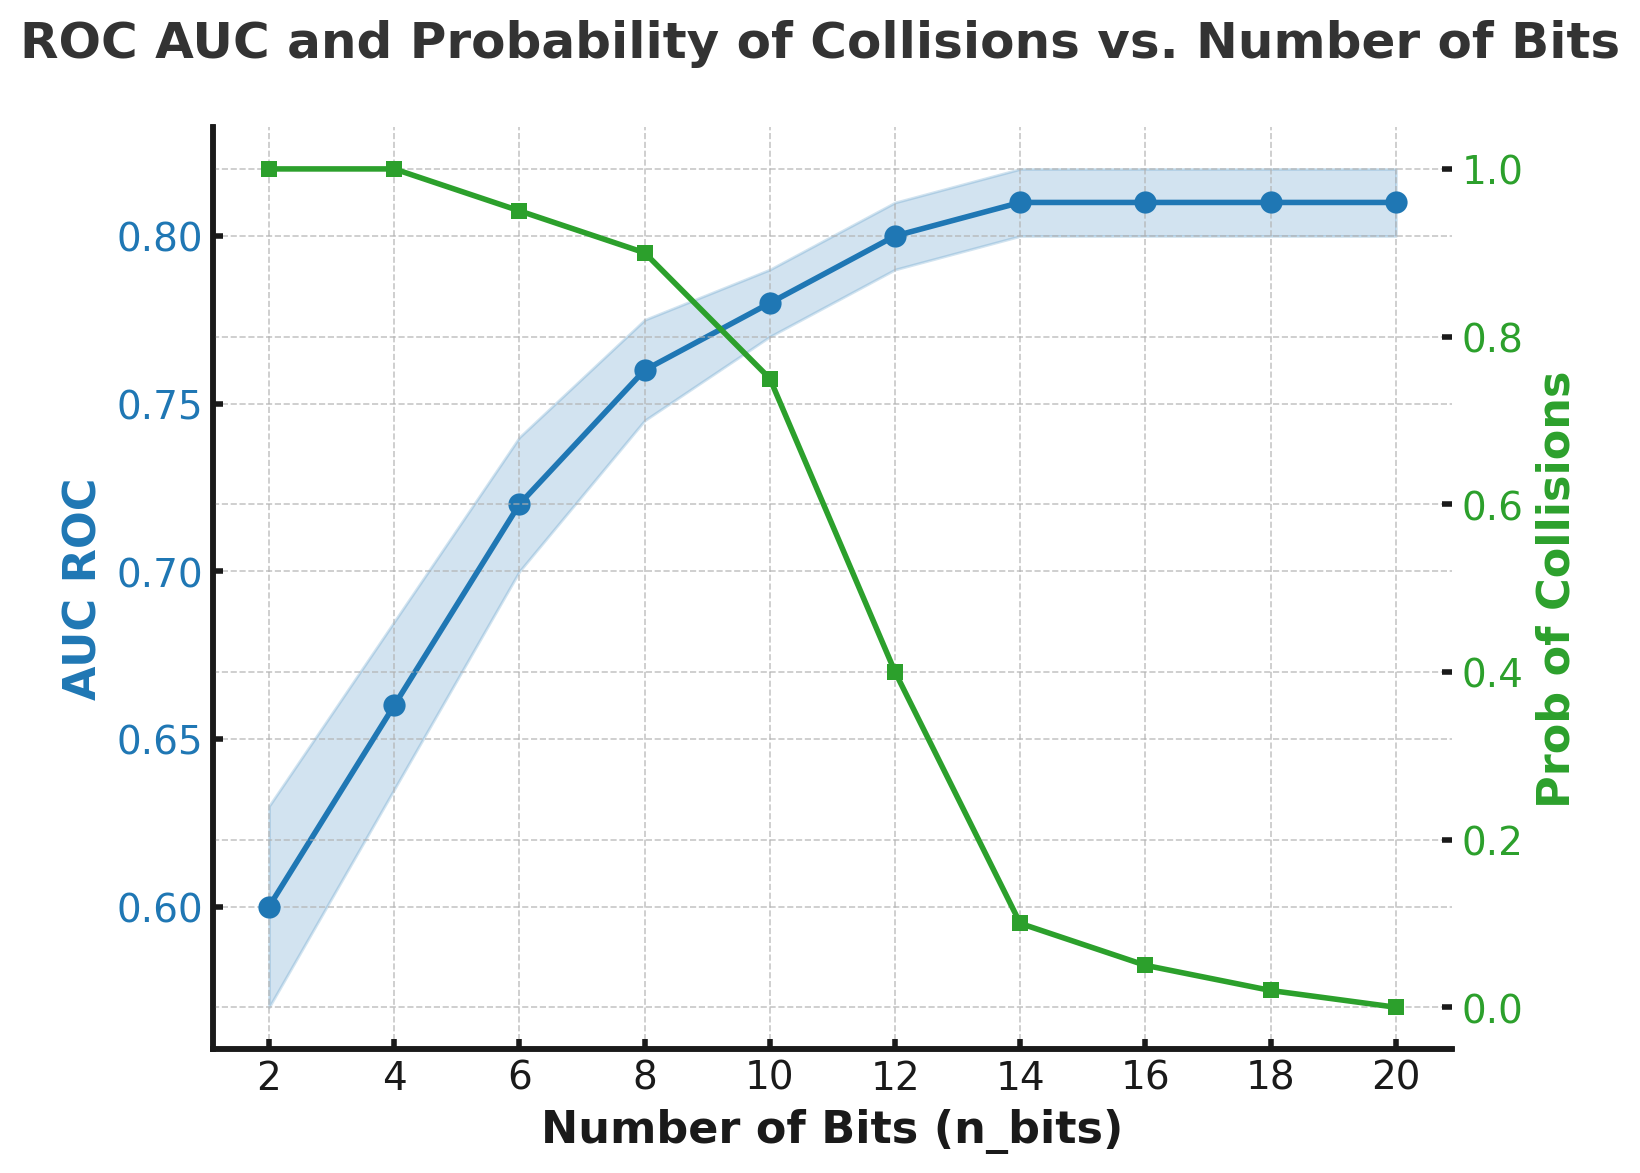
\includegraphics[
      width=\linewidth,
      trim=6 2 6 2,
      clip
    ]{images/nbit.png}
    \caption{Predictive performance vs.\ number of hash bits.}
    \label{fig:nbit-a}
  \end{subfigure}
  \hfill
  \begin{subfigure}[t]{0.50\linewidth}
    \centering
    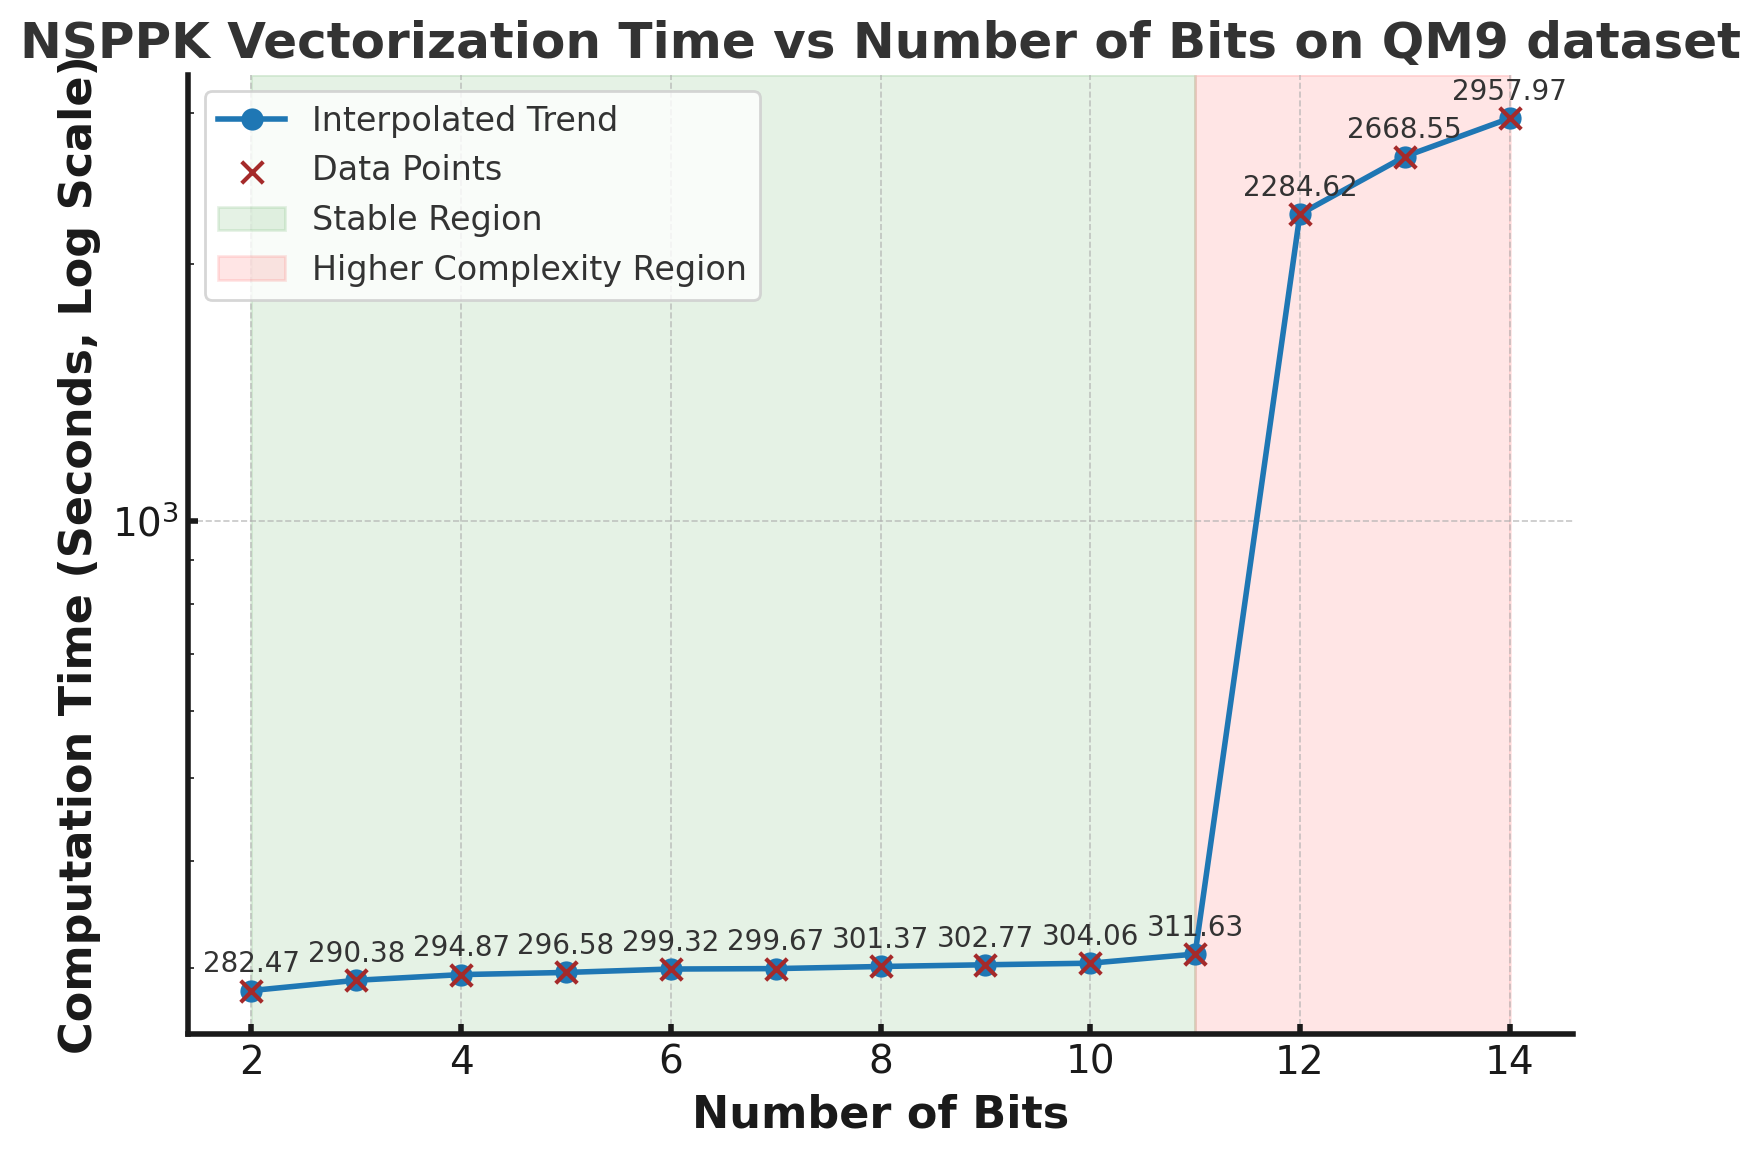
\includegraphics[width=\linewidth]{images/qm9_plot.png}
    \caption{NSPPK vectorisation time on QM9 vs.\ number of hash bits.}
    \label{fig:nsppk_qm9-a}
  \end{subfigure}

  \caption{Hash-size trade-offs: (a) predictive performance and (b) computational cost.}
  \label{fig:bits_tradeoff}
\end{figure}
\section{Diagonal Dominance and Robustness: Quantitative Analysis}
\label{sec:Diagonal}

A central pathology in similarity-based learning on graphs is the phenomenon of
\emph{diagonal dominance}. In this regime, the kernel matrix
$K\in\mathbb{R}^{N\times N}$ is dominated by its diagonal entries, with
$K_{ij}\approx 0$ for $i\neq j$. As a consequence, each graph is effectively
mapped to an isolated point, eliminating meaningful cross-graph similarity and
leading to poor generalisation and unstable optimisation. Prior work has shown
that R-convolution kernels are especially vulnerable to this effect, particularly
on graphs with high-dimensional or continuous attributes, where sparsity reduces
feature overlap even between mildly perturbed instances
\citep{gartner2003graph,shervashidze2009efficient,yanardag2015deep}.

To probe this issue, we perform a controlled robustness study. Starting from a
prototype graph $G_0$ with $n=200$ nodes, we generate a sequence of $50$
perturbed graphs $\{G_t\}_{t=1}^{50}$ through: (i) random node deletions and edge
removals while preserving connectivity, (ii) Gaussian noise injected into
five-dimensional node attributes, and (iii) a combined regime mixing structural
and attribute perturbations. For each method, we compute the full similarity
matrix $K_{ij}=k(G_i,G_j)$ across the perturbed graphs, allowing us to evaluate
both self-similarity decay and global structural preservation.

We benchmark NSPPK against five representative methods:
(1) \emph{GIN-Random} \citep{xu2019powerful}, a Graph Isomorphism Network with
random initialisation and no supervision;
(2) \emph{GraphCL} \citep{you2020graph}, a contrastive pretraining framework for
graph neural networks;
(3) \emph{InfoGraph} \citep{sun2019infograph}, an unsupervised GNN maximising
mutual information;
(4) \emph{GraphHopper} \citep{feragen2013scalable}, a shortest-path-based
kernel; and
(5) the \emph{Propagation Kernel (PK)} \citep{neumann2016propagation}, which
propagates and hashes node attributes.

Figure~\ref{fig:perturbation_panel}(a) shows the decay of normalised
self-similarity,
\[
\frac{K(G_0,G_t)}{K(G_0,G_0)},
\]
with increasing perturbation index $t$. An informative kernel should display
smooth decay: abrupt collapses indicate hypersensitivity, while nearly flat
trajectories suggest oversmoothing. GNN-based baselines such as GIN-Random and
GraphCL often remain nearly flat under structural perturbations, suggesting
insensitivity to fine-grained variation, while InfoGraph is only modestly more
responsive. In contrast, classical kernels such as GraphHopper and the
Propagation Kernel exhibit instability under attribute noise, with curves
collapsing or oscillating due to their reliance on path-based or propagation-based
dynamics. NSPPK achieves a well-calibrated, approximately monotonic decay across
all regimes, balancing sensitivity to structural changes with resilience to noise.

A complementary perspective comes from the pairwise similarity matrices in
Figure~\ref{fig:perturbation_panel}(b). Under Gaussian noise, GraphHopper and
the Propagation Kernel suffer severe diagonal dominance: bright diagonals and
small off-diagonal values indicate limited cross-graph similarity. Neural methods
such as GIN-Random, GraphCL, and InfoGraph avoid complete collapse, but often
produce oversmoothed matrices in which subtle distinctions are reduced. NSPPK
maintains dense, structured similarity patterns, avoiding diagonal collapse while
preserving discriminative variation across perturbed graphs.

\begin{figure}[t]
\centering

\begin{subfigure}[t]{0.49\linewidth}
\centering
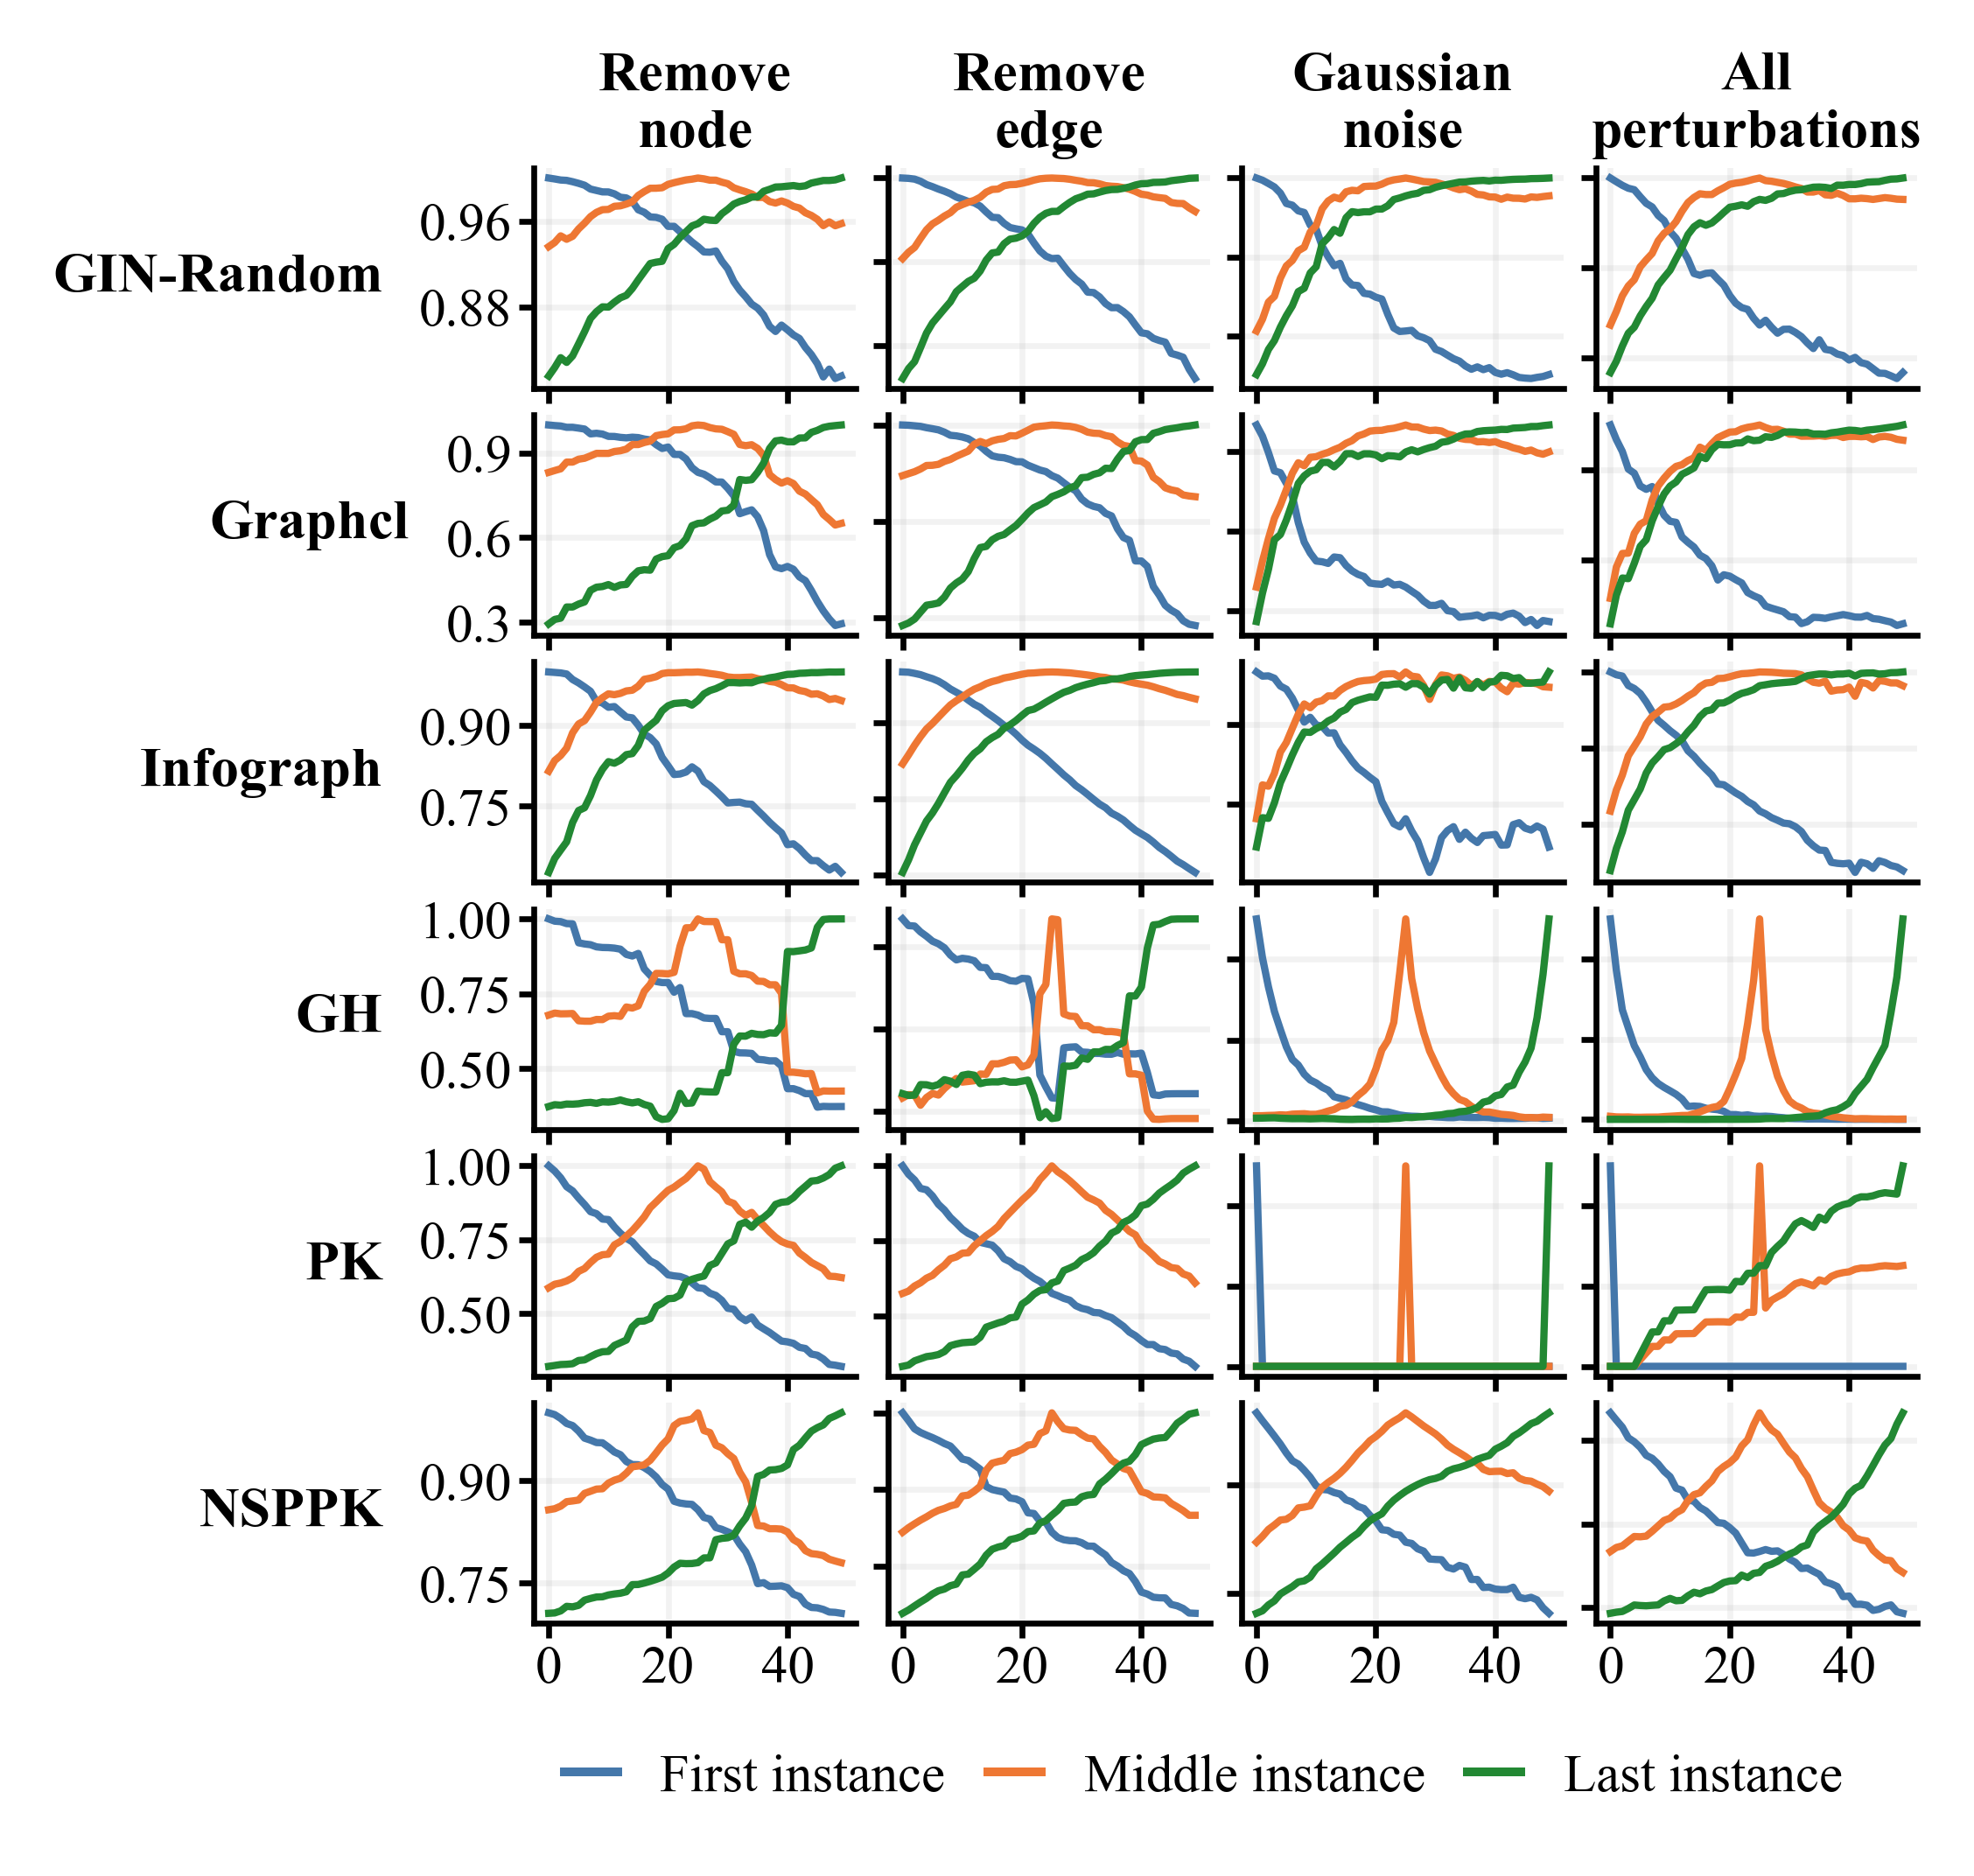
\includegraphics[width=\linewidth]{images/embedding_instance_similarity.png}
\caption{Instance similarity curves}
\label{fig:inst-curves}
\end{subfigure}
\hfill
\begin{subfigure}[t]{0.49\linewidth}
\centering
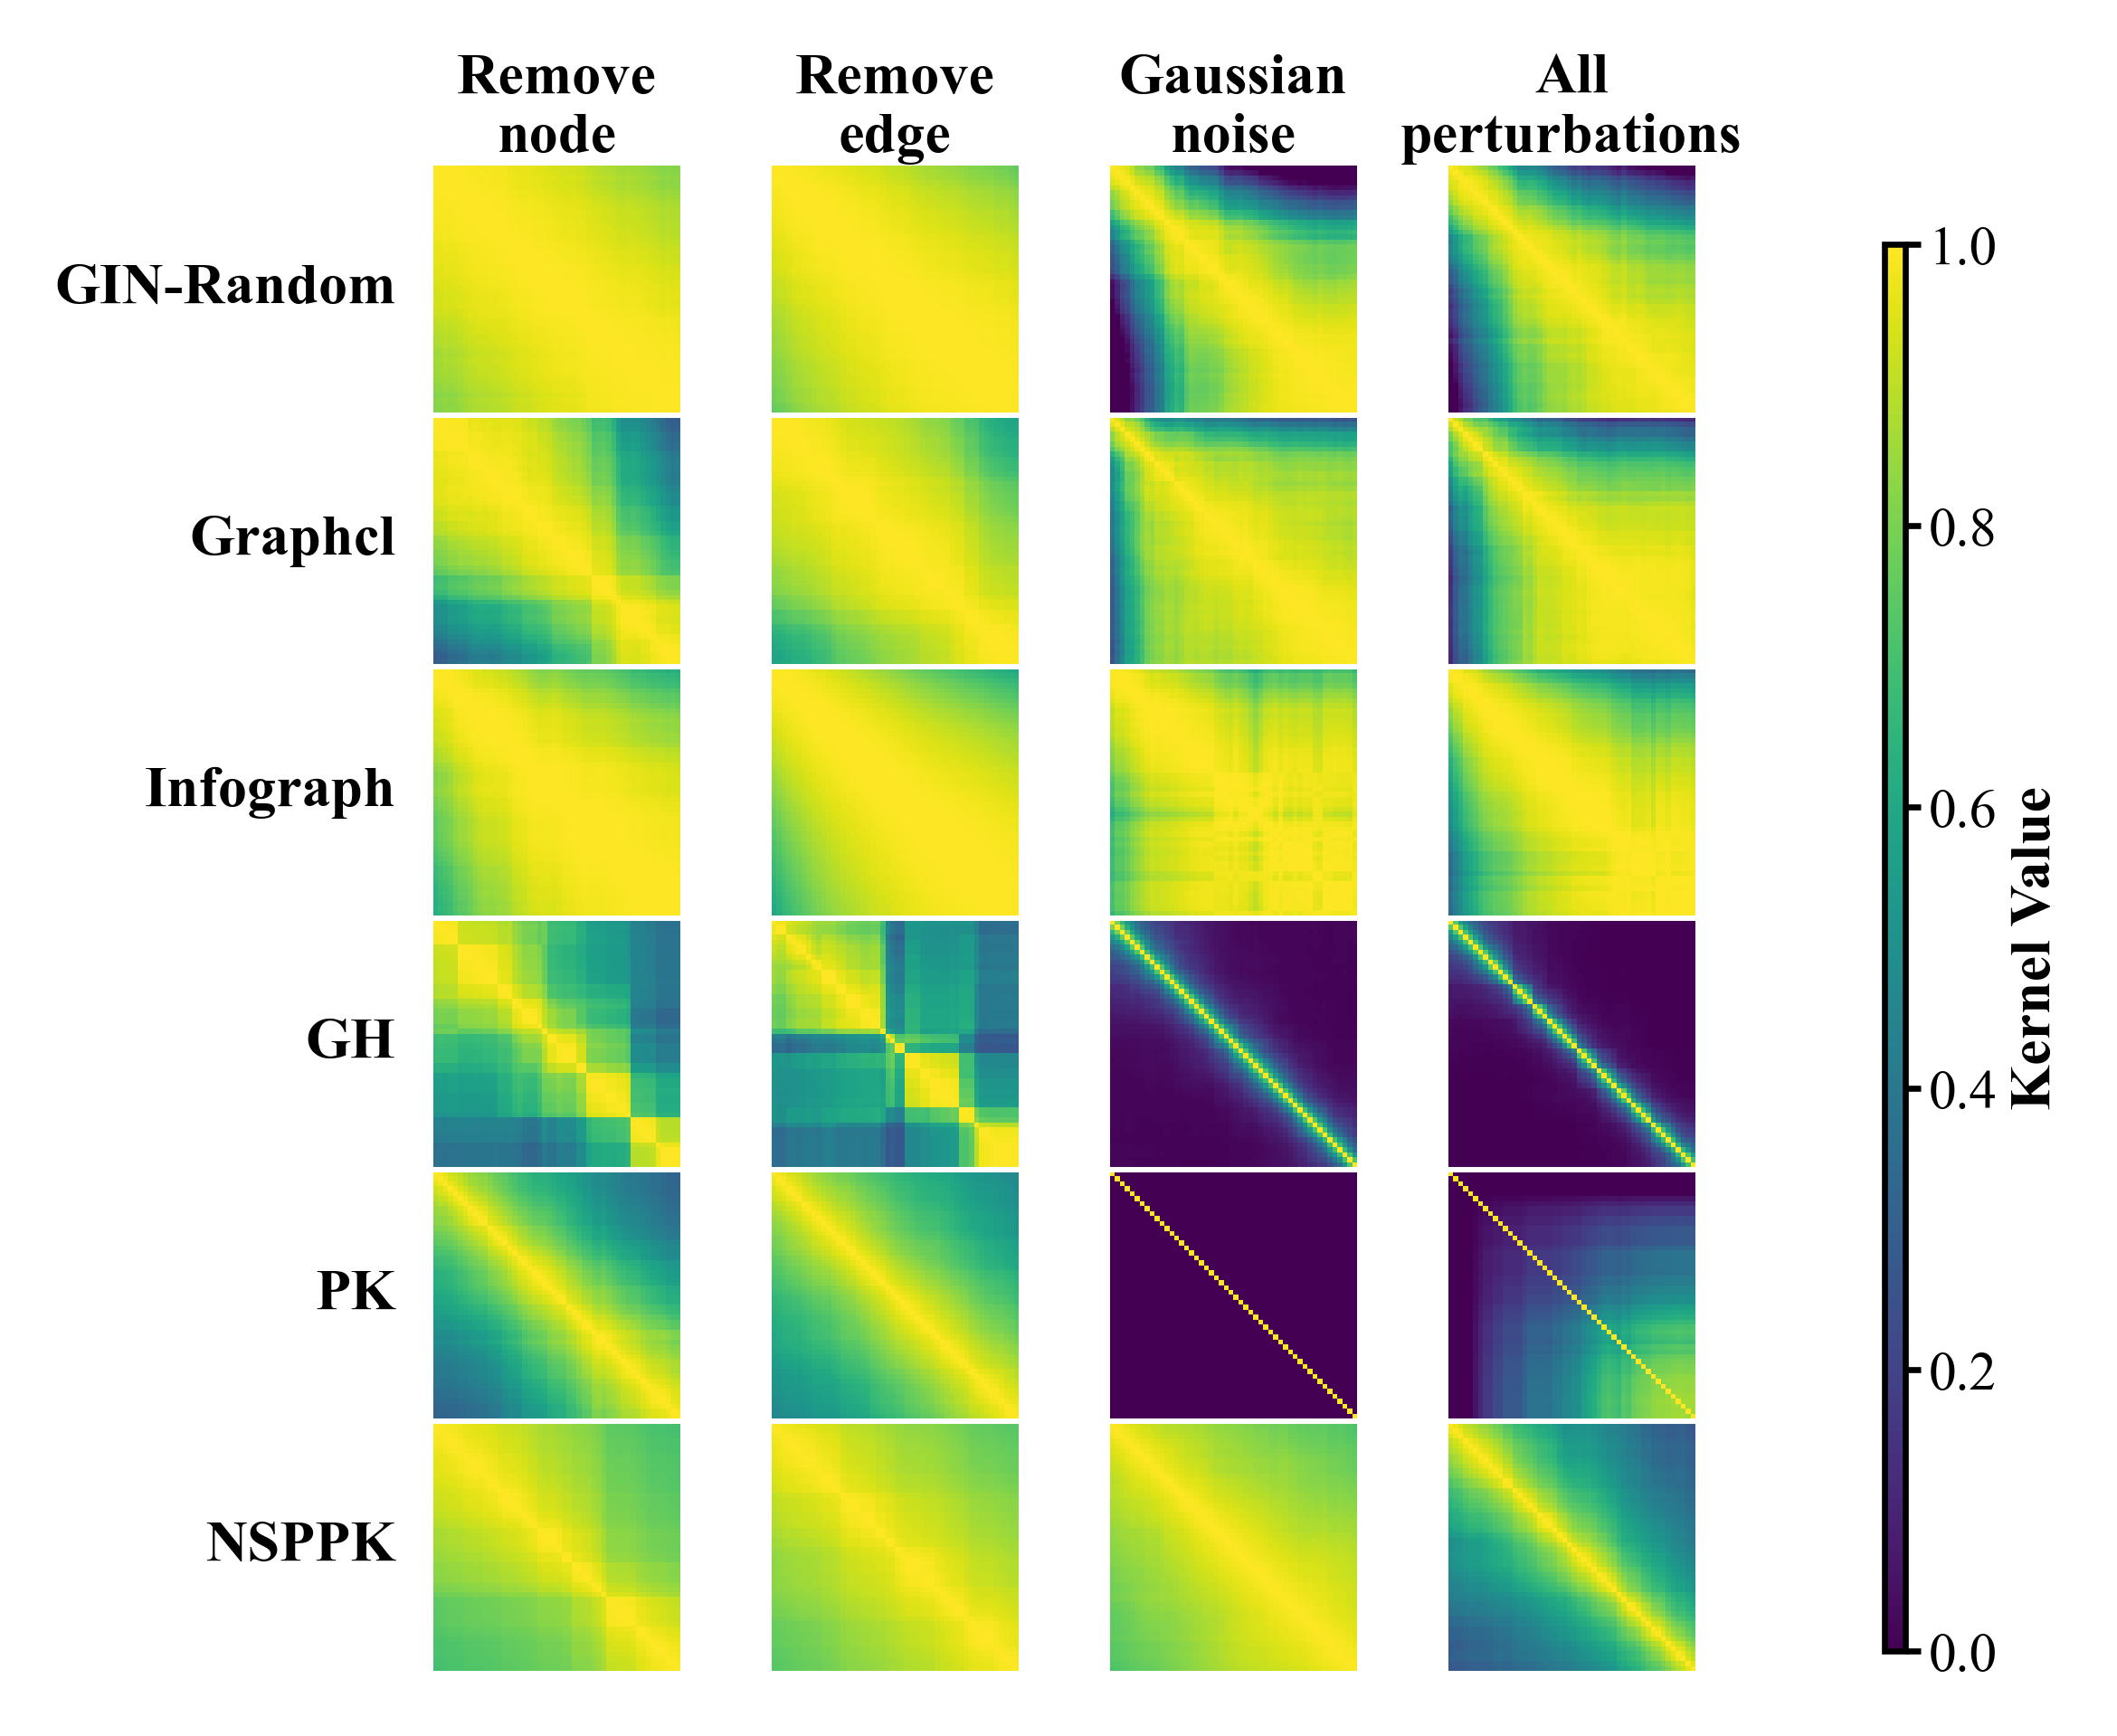
\includegraphics[width=\linewidth]{images/embedding_similarity.png}
\caption{Pairwise similarity matrices}
\label{fig:pairwise}
\end{subfigure}

\vspace{2mm}

\begin{subfigure}[t]{0.49\linewidth}
\centering
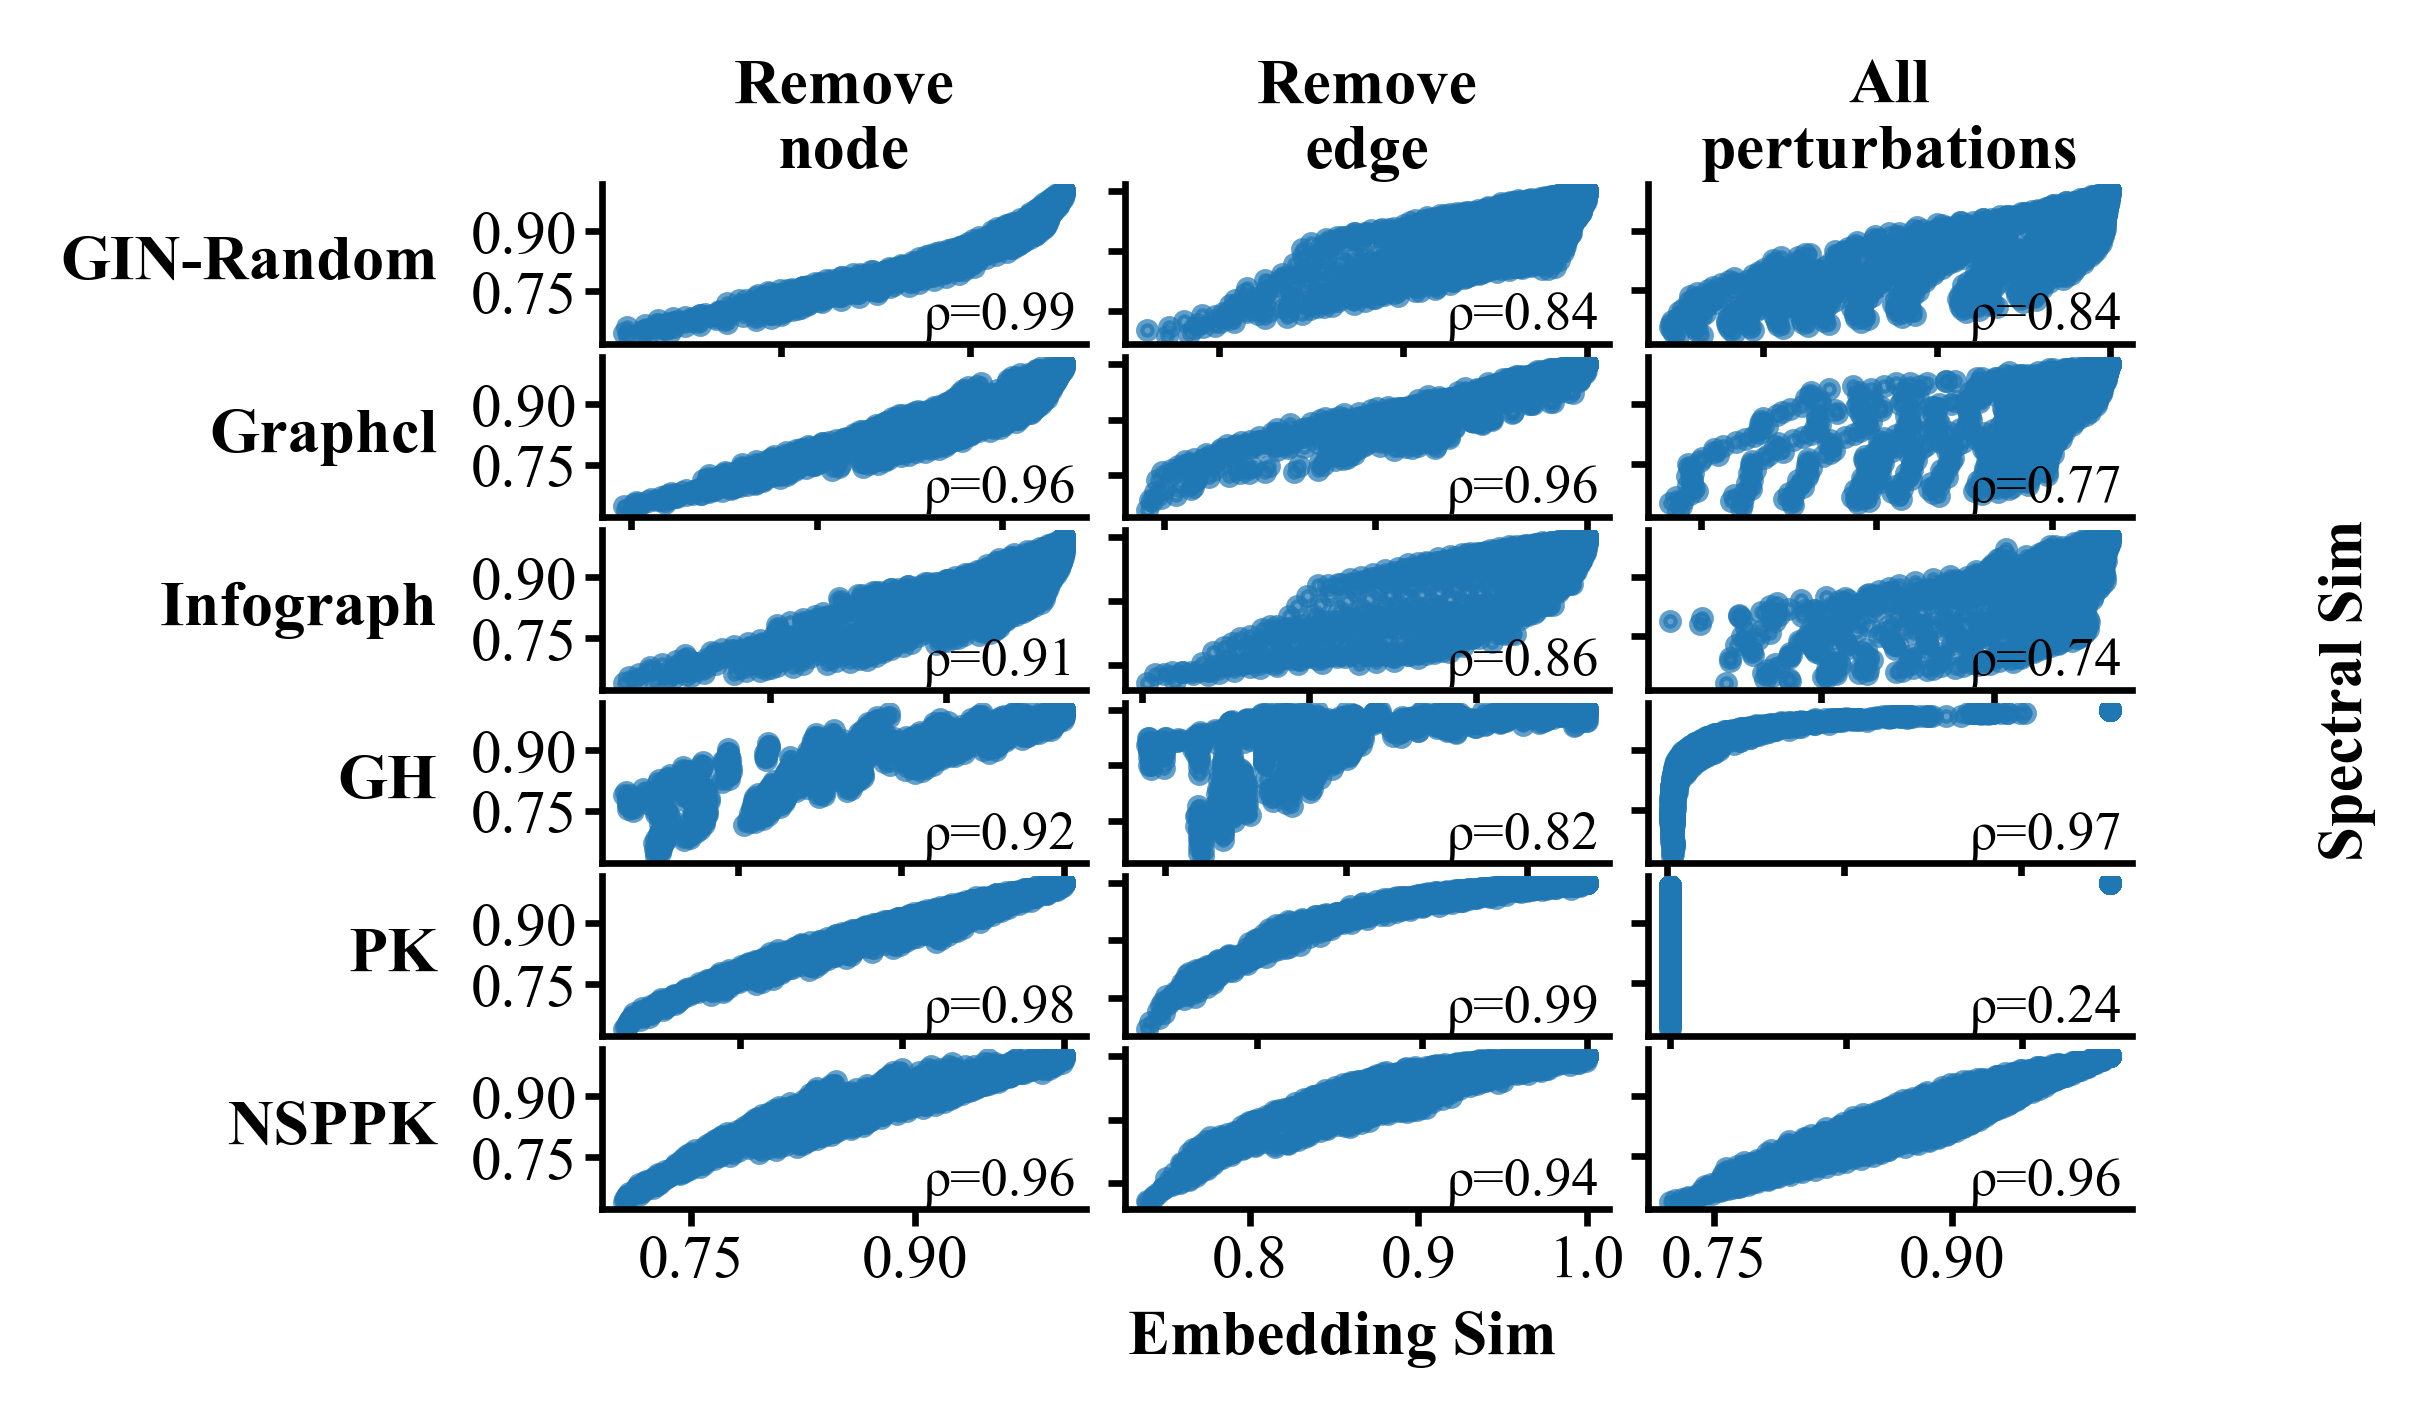
\includegraphics[width=\linewidth]{images/emb_vs_spec.png}
\caption{Embedding vs.\ spectral similarity (Spearman's $\rho$)}
\label{fig:emb-vs-spec}
\end{subfigure}
\hfill
\begin{subfigure}[t]{0.49\linewidth}
\centering
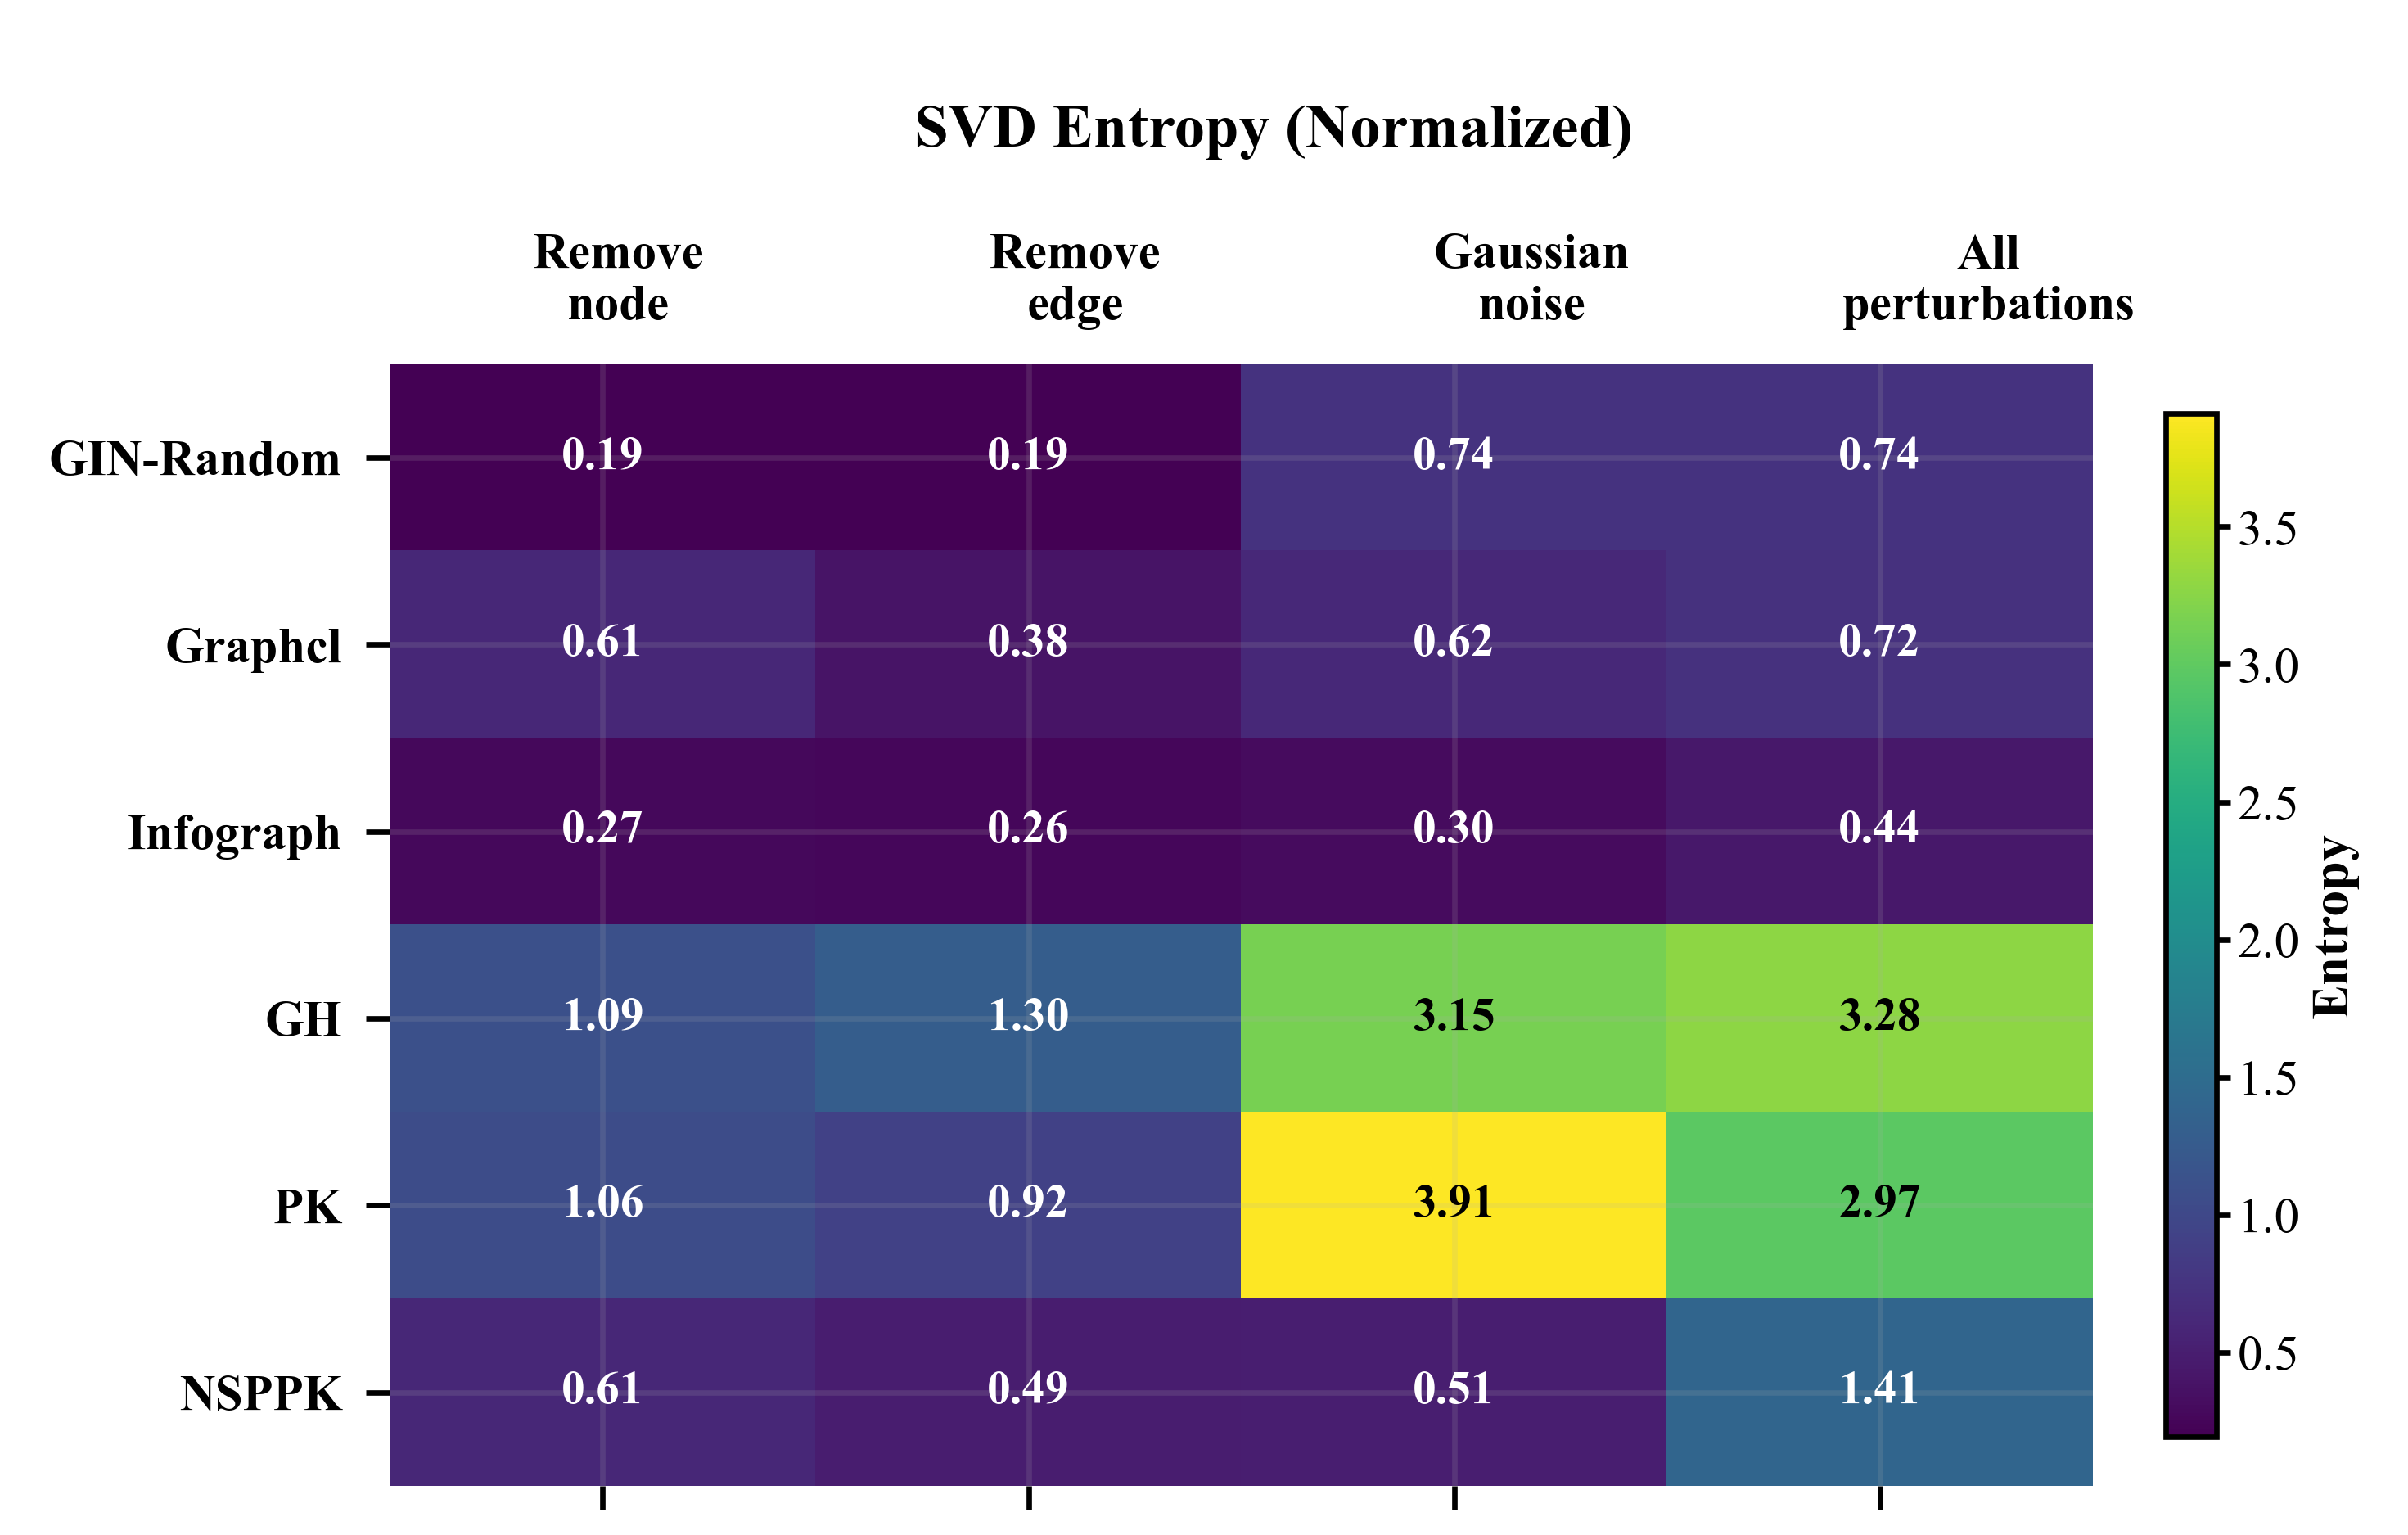
\includegraphics[width=\linewidth]{images/svd_entropy.png}
\caption{SVD entropy of similarity matrices}
\label{fig:svd-entropy}
\end{subfigure}

\caption{\textbf{Unified robustness analysis of graph similarity methods under perturbations.}
(a) Decay of self-similarity across perturbations.
(b) Pairwise similarity matrices showing diagonal dominance in baselines versus NSPPK.
(c) Correlation between kernel similarity and spectral similarity (Spearman $\rho$).
(d) SVD entropy of similarity matrices. NSPPK preserves stable, meaningful similarity structure, avoiding diagonal collapse.}
\label{fig:perturbation_panel}

\end{figure}

We further assess \emph{spectral alignment} by measuring the Spearman correlation
$\rho$ between kernel similarities and Laplacian spectral similarity
(Figure~\ref{fig:perturbation_panel}(c)). High $\rho$ indicates embeddings that
respect the intrinsic geometry of the graph family. NSPPK consistently achieves
high alignment across perturbations, while GNN-based methods perform
competitively but degrade under mixed noise, consistent with known oversmoothing
effects~\citep{kipf2017semi,oono2019graph,rong2020dropedge,balcilar2021analyzing}.
Classical kernels fare worse: the Propagation Kernel degrades under attribute
perturbations, and GraphHopper shows inconsistent alignment across regimes.

Finally, we quantify \emph{global expressivity} using normalised SVD entropy of
the similarity matrix,
\[
H_{\mathrm{SVD}} = -\sum_i \lambda_i \log \lambda_i.
\]
where $\{\lambda_i\}$ are the singular values of $K$ normalised to unit sum
(Figure~\ref{fig:perturbation_panel}(d)). Low entropy indicates spectral
degeneracy, where only a few singular directions explain most of the variation;
very high entropy may instead reflect instability or noise. Classical kernels can
exhibit unstable entropy under Gaussian noise, suggesting sensitivity to noisy
directions rather than genuine structural diversity. GNN baselines tend to yield
lower entropy, indicating stable but potentially under-expressive embeddings.
NSPPK maintains a high but stable entropy profile, reflecting a richer
similarity structure without diagonal collapse.

Taken together, these results show that NSPPK mitigates diagonal dominance while
preserving robustness and expressivity. Unlike prior kernels
\citep{shervashidze2009efficient,yanardag2015deep,neumann2016propagation} and
GNN methods \citep{xu2019powerful,yi2022graph,sun2019infograph}, which are prone
to either instability or oversmoothing under perturbation, NSPPK provides stable,
interpretable embeddings that respect spectral geometry and maintain
discriminative power.

\section{Experiments}
\label{sec:experiments}

\subsection{Small-Scale Datasets}
\label{sec:small_datasets}

We evaluate NSPPK against kernel and neural baselines on six node-attributed
graph classification benchmarks: \emph{ENZYMES},
\emph{PROTEINS\_full}, \emph{BZR}, \emph{COX2}, \emph{DHFR}, and
\emph{SYNTHETICnew}. Detailed dataset descriptions and summary statistics are
provided in Appendix~\ref{appendix:datasets}.


\textbf{Baselines.}
Kernel methods: GraphHopper (GH)~\citep{feragen2013scalable}, Propagation Kernel (PK)~\citep{neumann2016propagation}, Subgraph Matching (SM)~\citep{kriege2012subgraph}, Multiscale Laplacian (ML)~\citep{kondor2016multiscalelaplaciangraphkernel}, Shortest Path (SP)~\citep{borgwardt2005shortest}, HSSPK-SP/WL~\citep{morris2016fasterkernelsgraphscontinuous}, WWL~\citep{togninalli2019wasserstein}, linearFGW~\citep{nguyen2023linearfgw}, and NP~\citep{fang2023neighborhoodpreserving}, plus discretised NSPPK and WL.
All kernels use SVM classifiers (LIBSVM~\citep{chang2011libsvm}).

\textbf{Neural baselines}: DGCNN~\citep{zhang2018endtoend}, GraphSAGE~\citep{hamilton2017graphsage}, InfoGraph~\citep{sun2019infograph}, GIN~\citep{xu2019powerful}, GraphCL~\citep{you2020graph}, AttentiveFP (FNP)~\citep{gasteiger2020directional}, PNA~\citep{corso2020pna}, and PDF~\citep{yang2023bettergraphrepresentationlearning}.

\textbf{Protocol.}
We follow the fair evaluation setup of~\citep{errica2020fair}: 10-fold cross-validation with 10\% validation from training data.
Kernels: SVM with $C$ tuned on validation; multiple hyperparameter configurations tested; kernel computation times reported for best models.
GNNs: trained up to 1000 epochs with early stopping; tuned via validation.
The hyperparameter grids used for model selection for both neural and kernel baselines are reported in Appendix~\ref{appendix:hyperparameters}.

\textbf{Controls.}
We also test (i) \emph{attributes only}, where graphs are represented by summed node attributes, and (ii) \emph{structure only}, where attributes are removed (Appendix~\ref{appendix:no_attr}).

 \textbf{NSPPK}: fixed configuration across all datasets ($R{=}1,D{=}4,R'{=}1$, 16-bit hashing); no per-dataset tuning.
For comparison with kernels we use LIBSVM, and for GNNs we use NSPPK features with XGBoost.
All kernel runtimes, including NSPPK, are measured on a single CPU core for comparability.

\textbf{Runtime.}
Kernel methods run on a single CPU core; GNNs run on CPUs with library-level multithreading. All experiments used a SLURM-managed cluster with NVIDIA A100 GPUs, Intel Xeon Gold 5317 CPUs (24 cores), and 64 GB RAM. Kernels exceeding 24h per fold are reported as timeouts.



\begin{table}[t]
\centering
\caption{Classification accuracy (\%) with node attributes (+) and average rank.}
\label{tab:with_attr}
\scriptsize
\setlength{\tabcolsep}{3.2pt}
\begin{adjustbox}{max width=\textwidth}
\begin{tabular}{lccccccc}
\toprule
\textbf{Method} & \makecell{\textbf{SYNTHETIC}\\\textbf{new}} & \textbf{DHFR} & \textbf{BZR} & \textbf{COX2} & \textbf{ENZYMES} & \textbf{PROTEINS} & \textbf{Avg Rank} \\
\midrule
SM                      & \TO & \TO & \mps{83.96}{3.85} & \mps{78.81}{4.49} & \TO & \TO & ~8* \\
SP                      & \TO & \TO & \TO & \TO & \TO & \TO & -- \\
ML                      & \mps{50.33}{9.00} & \mps{78.57}{4.21} & \mps{82.96}{5.24} & \mps{77.53}{5.53} & \mps{36.33}{4.33} & \mps{72.06}{3.60} & 10.25 \\
PK                      & \mps{54.33}{10.11} & \mps{60.98}{0.48} & \mps{78.77}{1.01} & \mps{78.16}{8.07} & \mps{20.67}{2.70} & \mps{59.70}{0.16} & 12.58 \\
HSPPK\_WL               & \mps{60.33}{6.74} & \mps{77.38}{5.44} & \mps{85.67}{3.46} & \mps{80.30}{4.67} & \mps{60.17}{6.26} & \mps{72.96}{4.84} & 5.75\\
HSPPK\_SP               & \mps{57.00}{7.81} & \mps{77.40}{3.85} & \mps{84.49}{5.04} & \mps{80.31}{5.70} & \mps{58.50}{5.55} & \mps{68.55}{5.24} & 7.17 \\
GH                      & \mps{77.33}{7.42} & \mps{78.19}{5.47} & \mps{85.94}{5.17} & \mps{78.90}{2.95} & \mps{66.50}{6.17} & \mps{72.06}{3.64} & 4.75 \\
NP                      & \textbf{\mps{99.00}{2.13}} & \mps{80.42}{4.57} & \mps{86.18}{5.53} & \mps{78.16}{4.47} & \mps{43.00}{5.76} & \mps{64.62}{5.13} & 6.58 \\
linearFGW-RAW           & \mps{62.00}{8.46} & \mps{60.85}{3.75} & \mps{76.34}{5.68} & \mps{77.93}{3.68} & \mps{56.67}{7.07} & \mps{69.47}{0.91} & 10.83 \\
linearFGW-WL1           & \mps{72.33}{8.70} & \mps{59.94}{4.11} & \mps{78.52}{3.99} & \mps{72.13}{7.40} & \mps{47.00}{4.70} & \mps{59.66}{0.38} & 12.83 \\
linearFGW-WL2           & \mps{71.33}{7.48} & \mps{57.82}{5.48} & \mps{78.51}{2.98} & \mps{75.16}{3.34} & \mps{41.00}{7.57} & \mps{59.75}{0.43} & 13.00 \\
WL (disc.)              & \mps{88.33}{5.63} & \mps{77.26}{5.81} & \mps{83.71}{4.83} & \mps{77.10}{5.59} & \mps{50.67}{7.03} & \mps{71.16}{4.03} & 8.75 \\
WLOA                    & \mps{85.33}{5.62} & \mps{75.00}{3.23} & \mps{84.20}{4.47} & \mps{74.54}{5.40} & \mps{66.33}{5.21} & \mps{71.16}{1.97} & 8.08 \\
WWL                     & \mps{58.33}{7.78} & \mps{77.12}{3.58} & \mps{86.45}{4.50} & \mps{79.03}{3.84} & \textbf{\mps{73.67}{5.26}} & \textbf{\mps{77.18}{5.27}} & 4.83 \\
NSPDK (disc.)           & \mps{96.33}{3.14} & \mps{82.93}{5.56} & \mps{85.70}{3.90} & \mps{80.30}{4.15} & \mps{52.67}{4.67} & \mps{72.87}{1.51} & 4.42 \\
\rowcolor{gray!10}
NSPPK (ours)            & \textbf{\mps{99.00}{1.52}} & \textbf{\mps{82.95}{4.57}} & \textbf{\mps{87.17}{3.58}} & \mps{81.16}{2.30} & \mps{60.50}{5.38} & \mps{74.66}{3.81} & \textbf{1.75} \\
\midrule
\emph{Attributes only}  & \mps{54.33}{9.55} & \mps{60.98}{4.80} & \mps{78.77}{1.01} & \mps{78.16}{8.07} & \mps{55.67}{5.38} & \mps{62.80}{2.52} & 11.50 \\
\bottomrule
\end{tabular}
\end{adjustbox}

\vspace{0.5ex}
{\footnotesize\emph{Note:} ``Attributes only'' participates in Avg Rank like any other method.}
\end{table}

% ========================= NEURAL NETS — WITH ATTRIBUTES =========================
\begin{table}[t]
\centering
\caption{Neural networks: classification accuracy (\%) with node attributes (+) and Avg Rank.}
\label{tab:nn_with_attr}
\scriptsize
\setlength{\tabcolsep}{3.2pt}
\begin{adjustbox}{max width=\textwidth}
\begin{tabular}{lccccccc}
\toprule
\textbf{Method} & \textbf{\makecell{SYNTHETIC\\new}} & \textbf{DHFR} & \textbf{BZR} & \textbf{COX2} & \textbf{ENZYMES} & \textbf{PROTEINS} & \textbf{Avg Rank} \\
\midrule
DGCNN                & \mps{46.67}{5.63} & \mps{68.77}{5.52} & \mps{79.40}{3.32} & \mps{77.15}{0.06} & \mps{33.33}{9.37} & \mps{73.86}{3.56} & 10.58 \\
GraphSAGE            & \mps{76.67}{7.70} & \mps{76.46}{4.13} & \mps{83.70}{4.44} & \mps{80.93}{0.07} & \mps{65.00}{5.73} & \mps{75.02}{3.29} & 4.42 \\
InfoGraph            & \mps{65.00}{16.05} & \mps{73.01}{6.03} & \mps{79.01}{3.42} & \mps{77.77}{14.20} & \mps{53.33}{7.84} & \mps{66.37}{6.25} & 7.25 \\
GIN                  & \mps{83.67}{5.92} & \mps{76.85}{7.23} & \mps{84.17}{6.14} & \mps{81.80}{6.14} & \textbf{\mps{68.30}{5.43}} & \mps{62.10}{5.26} & 4.33\\
GraphCL              & \mps{67.00}{9.48} & \mps{80.34}{6.95} & \mps{84.17}{3.62} & \mps{80.34}{6.95} & \mps{48.17}{6.93} & \mps{75.82}{2.73} & 5.17 \\
GNN                  & \mps{64.67}{7.92} & \mps{76.59}{6.97} & \mps{85.66}{4.60} & \mps{79.92}{7.08} & \mps{65.17}{8.41} & \mps{66.57}{6.10} & 5.50 \\
FNP                  & \mps{53.33}{11.16} & \mps{70.76}{3.99} & \mps{79.49}{3.94} & \mps{78.22}{7.01} & \mps{32.17}{12.98} & \mps{70.17}{3.15} & 9.42 \\
PNA                  & \mps{55.67}{20.66} & \mps{61.50}{5.42} & \mps{79.01}{4.33} & \mps{78.22}{7.02} & \mps{20.83}{7.12} & \mps{75.11}{3.60} & 8.17 \\
PDF                  & \mps{97.67}{2.60} & \mps{77.37}{4.50} & \mps{83.68}{3.81} & \mps{82.23}{7.00} & \mps{65.00}{4.65} & \mps{72.14}{4.48} & 3.75 \\
\rowcolor{gray!10}
NSPPK feat.\ (XGBoost) & \textbf{\mps{98.67}{2.21}} & \textbf{\mps{83.74}{4.14}} & \textbf{\mps{88.66}{2.89}} & \textbf{\mps{82.90}{4.39}} & \mps{60.17}{6.30} & \textbf{\mps{77.37}{4.80}} & \textbf{1.67} \\
\midrule
\emph{Attributes only} & \mps{54.33}{9.55} & \mps{60.98}{ 4.80}& \mps{78.77}{1.01} & \mps{78.16}{8.07} & \mps{55.67}{5.38} & \mps{62.80}{2.52} & 7.75 \\
\bottomrule
\end{tabular}
\end{adjustbox}
\end{table}


\subsubsection{Runtime and Efficiency}
\label{sec:runtime}


Against \emph{kernels}, NSPPK achieves the best accuracy on four out of six
benchmarks (\emph{SYNTHETICnew}, \emph{BZR}, \emph{COX2},\emph{DHFR}) and the best overall
average rank (1.75 vs >4 for other kernels).
Under a conservative single-core evaluation setting, NSPPK delivers a favourable
efficiency--accuracy trade-off among kernel methods. Very lightweight baselines
such as GraphCL or PNA achieve lower runtimes (average rank $7.50$), but NSPPK
remains substantially more efficient than expressive graph kernels such as GH or
HSPPK, while consistently achieving higher predictive accuracy. When paired with
XGBoost, NSPPK delivers the strongest overall accuracy among kernel-based
methods.
Detailed runtime measurements are reported in
Tables~\ref{tab:with_attr_runtime_kernels} and~\ref{tab:with_attr_runtime_nns}.
Overall, NSPPK provides a favourable efficiency--accuracy trade-off,
achieving substantially higher accuracy than lightweight kernels while
remaining significantly more efficient than high-expressivity methods.
Additional visualizations of the accuracy--time trade-off across datasets
are provided in Appendix~\ref{appendix:tradeoff}.


\begin{table}[H]
\centering
\caption{Runtime (seconds) \textbf{with} node attributes (\textbf{lower is better}).}
\scriptsize
\label{tab:with_attr_runtime_kernels}
\setlength{\tabcolsep}{3.5pt}
\begin{adjustbox}{max width=\textwidth}
\begin{tabular}{lcccccccc}
\toprule
\textbf{Method} & \makecell{\textbf{SYNTHETIC}\\\textbf{NEW}} & \textbf{DHFR} & \textbf{BZR} & \textbf{COX2} & \textbf{ENZYMES} & \textbf{PROTEINS} & \textbf{Avg} & \textbf{Rank}\\
\midrule
SM & \TO & \TO & 12274.00\,s & 25927.96\,s & \TO & \TO & 19100.98\,s & 15.00\\
ML & 1777.93\,s & 1361.75\,s & 849.20\,s & 1155.49\,s & 1295.99\,s & 3628.70\,s & 1678.18\,s & 13.83\\
PK & 1.81\,s & 2.82\,s & 0.79\,s & 1.13\,s & 3.14\,s & 4.48\,s & 2.36\,s & \textbf{1.33}\\
HSPPK\_WL & 49.54\,s & 51.49\,s & 8.63\,s & 16.38\,s & 25.20\,s & 89.90\,s & 40.19\,s & 9.33\\
HSPPK\_SP & 249.75\,s & 63.1\,s & 16.52\,s & 29.22\,s & 28.35\,s & 119.32\,s & 84.38\,s & 11.00\\
GH & 242.05\,s & 318.8\,s & 112.43\,s & 132.63\,s & 365.25\,s & 3647.21\,s & 803.06\,s & 13.00\\
NP & 41.57\,s & 217.54\,s & 42.32\,s & 69.80\,s & 17.69\,s & 49.58\,s & 73.08\,s & 10.00\\
linearFGW-RAW & 6.82\,s & 22.14\,s & 6.63\,s & 9.84\,s & 8.73\,s & 69.67\,s & 20.64\,s & 5.50\\
linearFGW-WL1 & 6.94\,s & 22.58\,s & 5.89\,s & 10.75\,s & 8.29\,s & 67.19\,s & 20.27\,s & 5.50\\
linearFGW-WL2 & 5.95\,s & 25.23\,s & 7.02\,s & 10.92\,s & 10.26\,s & 71.63\,s & 21.84\,s & 6.50\\
WL (disc.) & 12.33\,s & 0.21\,s & 4.00\,s & 14.00\,s & 9.00\,s & 20.00\,s & 9.92\,s & 5.00\\
WLOA & 0.99\,s & 10.49\,s & 0.83\,s & 3.27\,s & 4.24\,s & 12.67\,s & 5.42\,s & 2.75\\
WWL & 29.96\,s & 105.03\,s & 14.71\,s & 40.89\,s & 32.54\,s & 134.95\,s & 59.68\,s & 10.67\\
NSPDK (disc.) & 6.50\,s & 10.49\,s & 4.69\,s & 2.64\,s & 3.18\,s & 6.13\,s & 5.61\,s & 3.08\\
\rowcolor{gray!10}
\textbf{NSPPK (ours)} & 34.81\,s & 36.19\,s & 12.75\,s & 12.75\,s & 26.45\,s & 5.73\,s & 21.45\,s & 7.50\\
\bottomrule
\end{tabular}
\end{adjustbox}
\end{table}

% ========================= RUNTIMES: NEURAL (WITH ATTRS) =========================
% ========================= RUNTIMES: NEURAL (WITH ATTRS) =========================
\begin{table}[H]
\centering
\caption{Neural runtimes (seconds) \textbf{with} node attributes (\textbf{lower is better}).}
\label{tab:with_attr_runtime_nns}
\scriptsize
\setlength{\tabcolsep}{3.5pt}
\begin{adjustbox}{max width=\textwidth}
\begin{tabular}{lcccccccc}
\toprule
\textbf{Method} & \makecell{\textbf{SYNTHETIC}\\\textbf{NEW}} & \textbf{DHFR} & \textbf{BZR} & \textbf{COX2} & \textbf{ENZYMES} & \textbf{PROT} & \textbf{Avg} & \textbf{Rank}\\
\midrule
DGCNN & 443.59\,s & 2956.95\,s & 304.88\,s & 704.74\,s & 948.88\,s & 1512.29\,s & 1145.22\,s & 9.83\\
GraphSAGE & 139.94\,s & 101.76\,s & 175.30\,s & 118.97\,s & 317.84\,s & 394.02\,s & 174.79\,s & 7.33\\
InfoGraph & 39.25\,s & 163.79\,s & 40.40\,s & 111.40\,s & 59.95\,s & 85.72\,s & 83.09\,s & 5.00\\
GIN & 474.24\,s & 1066.25\,s & 302.44\,s & 579.86\,s & 369.06\,s & 742.46\,s & 578.44\,s & 9.17\\
GraphCL & 11.33\,s & 5.11\,s & 4.10\,s & 5.11\,s & 15.51\,s & 20.04\,s & 10.34\,s & \textbf{1.17}\\
GNN & 165.92\,s & 242.21\,s & 100.28\,s & 153.89\,s & 207.18\,s & 371.30\,s & 207.35\,s & 7.50\\
FNP & 49.97\,s & 71.08\,s & 18.72\,s & 22.23\,s & 60.51\,s & 57.51\,s & 43.32\,s & 4.17\\
PNA & 16.67\,s & 27.45\,s & 4.38\,s & 3.86\,s & 17.33\,s & 22.14\,s & 17.12\,s & 1.83\\
PDF & 20.59\,s & 57.84\,s & 21.10\,s & 20.13\,s & 61.43\,s & 76.70\,s & 44.13\,s & 4.33\\
\rowcolor{gray!10}
\textbf{NSPPK feat.\ (XGB)} & 39.35\,s & 33.10\,s & 19.38\,s & 20.62\,s & 39.54\,s & 131.96\,s & 54.11\,s & 4.83\\
\bottomrule
\end{tabular}
\end{adjustbox}
\end{table}

\textbf{Results}

To complement the per-dataset accuracy and runtime tables, we summarise
performance across datasets using \emph{critical difference (CD) diagrams} based
on average normalised ranks with statistical testing
(Figures~\ref{fig:cd_kernels} and~\ref{fig:cd_nn}). Following the standard
block-design protocol, each dataset is treated as a block and methods are ranked
within each dataset according to accuracy. The ranks are then normalised to
$[0,1]$, with larger values indicating better performance, and averaged across
datasets to produce the aggregate score shown on the horizontal axis.

Statistical significance is assessed using the Friedman omnibus test, followed—when significant—by Conover post-hoc pairwise comparisons with Holm correction for multiple testing. In the CD diagrams, methods positioned further right achieve better average ranks, while methods connected by a shared crossbar belong to a non-significant group.

Figure~\ref{fig:cd_kernels} presents results for kernel methods only. NSPPK achieves the highest average rank, indicating consistently strong performance across datasets rather than isolated gains. Figure~\ref{fig:cd_nn} shows the corresponding diagram for neural baselines and the NSPPK feature pipeline. NSPPK feat.~(XGBoost) attains the best average rank, demonstrating that explicit NSPPK representations paired with lightweight downstream learners remain competitive with—and often outperform—end-to-end graph neural networks on node-attributed graph classification tasks.
\begin{figure}[t]
  \centering
  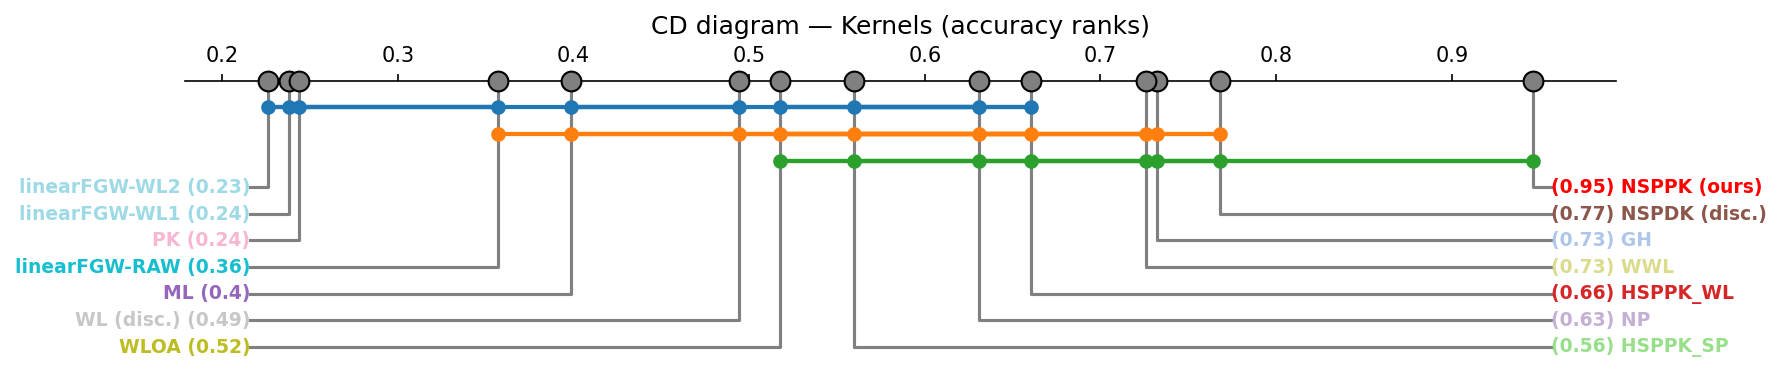
\includegraphics[width=\linewidth]{images/critical_difference_diagram_kernels.png}
\caption{Critical difference diagram for \textbf{kernel} methods on accuracy.
The horizontal axis shows average normalised rank across datasets, scaled to
$[0,1]$ so that higher values indicate better performance. Non-significant
groups under Conover post-hoc testing (Holm-corrected) are indicated by shared
crossbars.}
  \label{fig:cd_kernels}
\end{figure}

\begin{figure}[t]
  \centering
  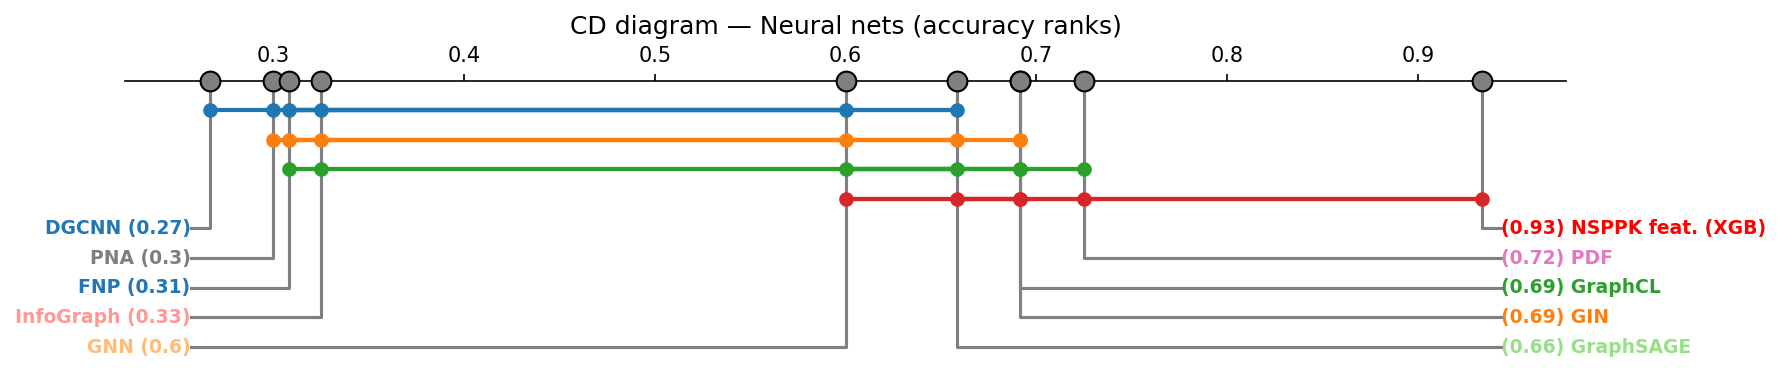
\includegraphics[width=\linewidth]{images/critical_difference_diagram_nn.png}
\caption{Critical difference diagram for \textbf{neural} baselines and the
NSPPK-feature pipeline on accuracy. The horizontal axis shows average normalised
rank across datasets, scaled to $[0,1]$ so that higher values indicate better
performance. Non-significant groups under Conover post-hoc testing
(Holm-corrected) are indicated by shared crossbars.}
  \label{fig:cd_nn}
\end{figure}




\subsection{Parallel Scalability}
\label{sec:parallel}

To evaluate NSPPK's scalability, we vectorized the \textbf{QM9} dataset (\textasciitilde130,000 graphs) using a fixed configuration: \textbf{12-bit hash size}, maximum \textbf{radius = 1}, \textbf{distance = 4}, and \textbf{connector path = 1}. This setup balances expressiveness and efficiency, making it suitable for large-scale benchmarks. As shown in Figure~\ref{fig:appendix_scaling_plot}, the total vectorisation time decreases almost linearly with the number of CPU cores, completing in under 10 minutes on 112 cores. This confirms NSPPK's efficient parallelization and practicality for large datasets.

Figure~\ref{fig:appendix_scaling_plot} presents the results on a log-log scale. The x-axis indicates the number of CPU cores, and the y-axis shows the total vectorisation time. The observed trend is close to ideal linear scaling: doubling the number of cores results in approximately half the runtime. This demonstrates that NSPPK's feature extraction process incurs minimal synchronization or coordination overhead.

Experiments were conducted on a dual-socket Intel server equipped with 2× Intel Xeon Gold 6330 CPUs @ 2.00 GHz, each providing 28 physical cores (56 threads), for a total of 112 logical CPU cores. The machine had 2 NUMA nodes, 70 MB of shared L2 cache, and 84 MB of L3 cache.
Despite relying solely on CPU resources, NSPPK scaled efficiently across all available cores. For example, complete vectorisation of the QM9 dataset was achieved in under 10 minutes, demonstrating the method’s practicality for real-world, large-scale deployment.

\begin{figure}[H]
  \centering
  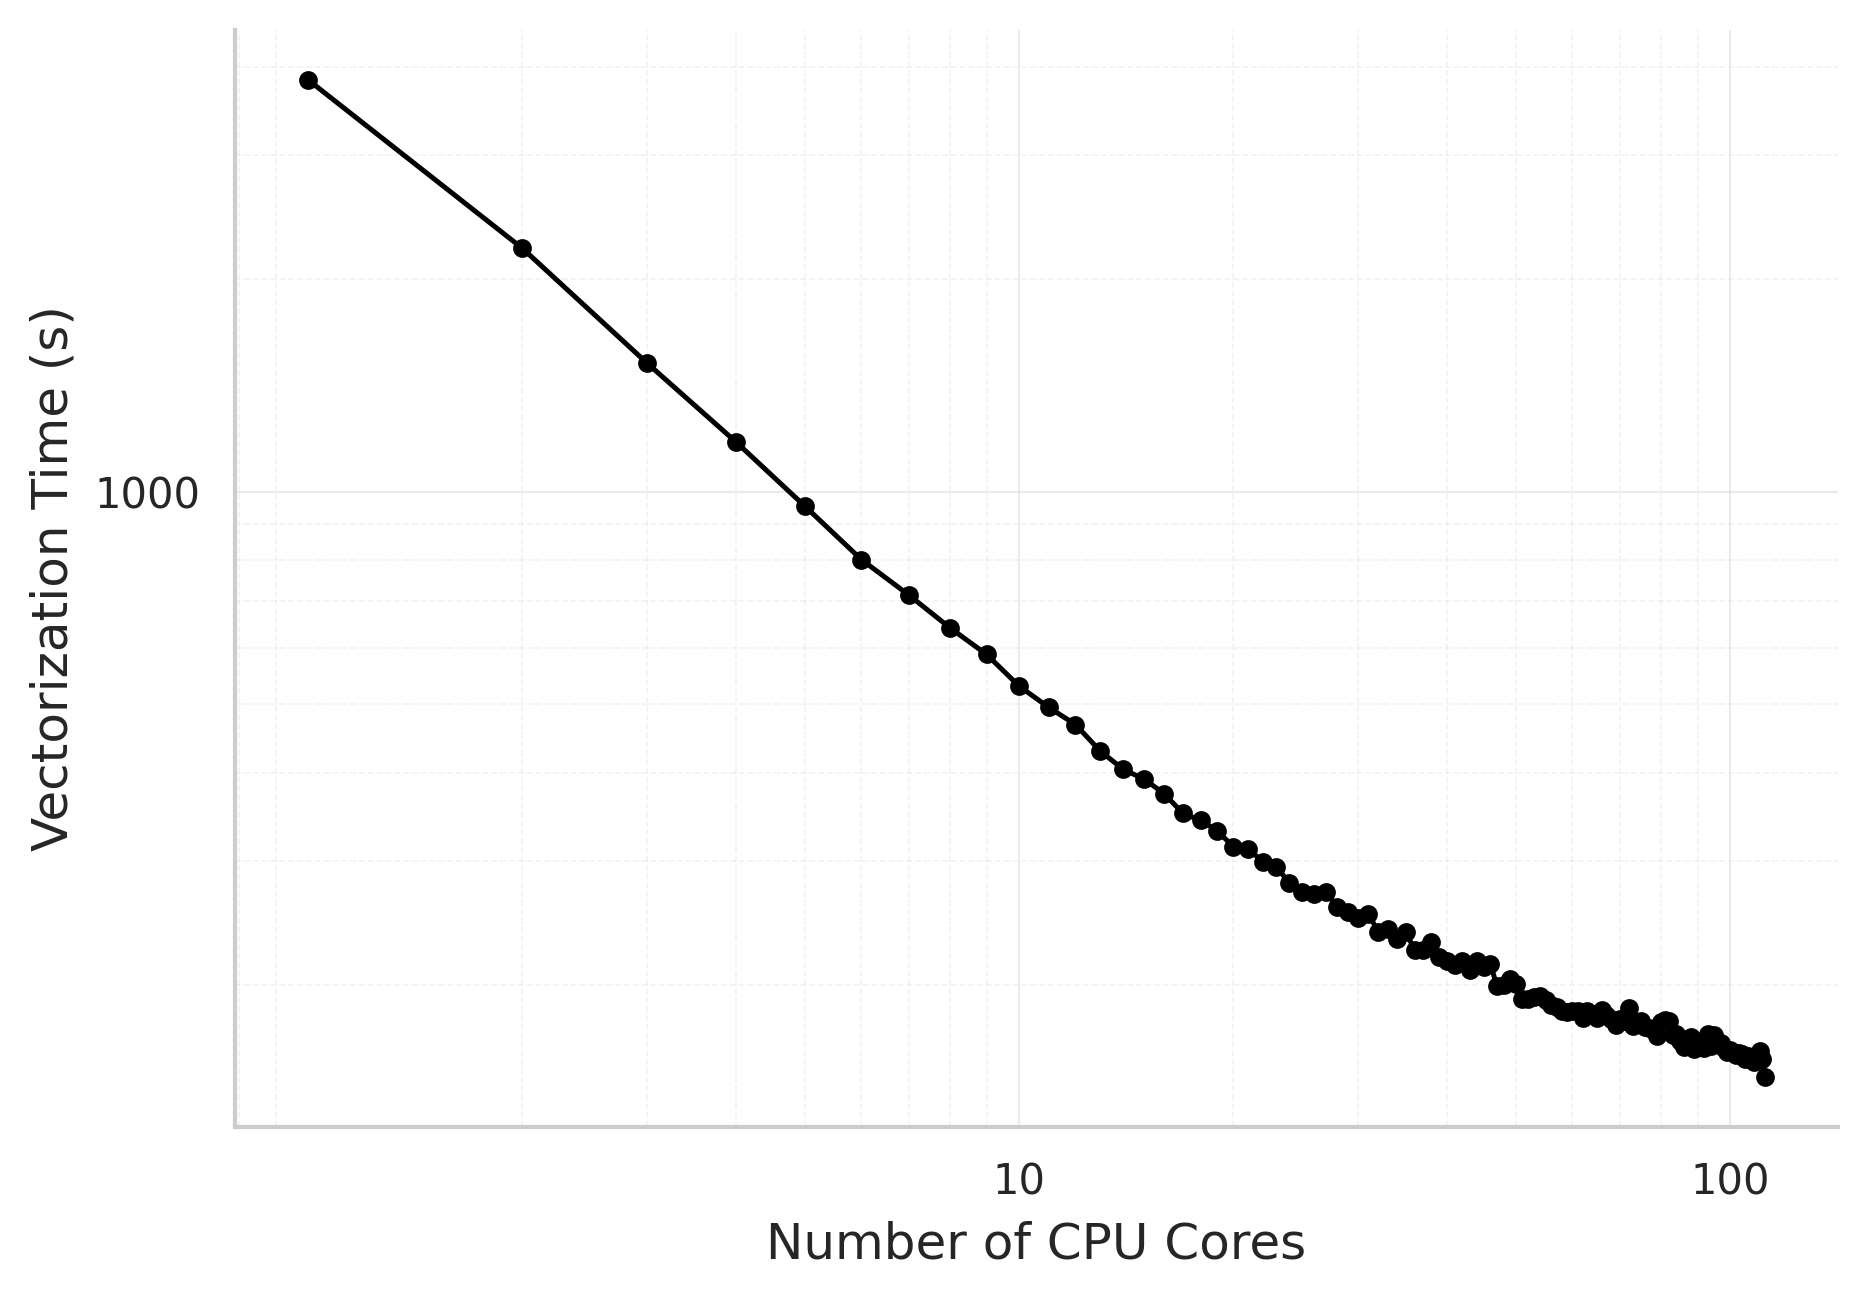
\includegraphics[width=0.5\linewidth]{images/output.png}
  \caption{vectorisation time vs.\ number of CPU cores on QM9 (log-log scale). NSPPK demonstrates excellent parallel scalability, reducing total vectorisation time from over an hour (using a single core) to under 10 minutes with 112 CPU cores. This shows near-linear performance gains with increased parallelization.}
  \label{fig:appendix_scaling_plot}
\end{figure}

\subsection{Ablation Study}
\label{sec:ablation}

We evaluate the contribution of three core components of NSPPK:
(i) distance-based features,
(ii) the union-of-shortest-paths connector, and
(iii) the high-degree thresholding heuristic.
All experiments use a fixed configuration ($R=1$, $D=4$, $r'=1$) with a
\texttt{RandomForestClassifier}.
Table~\ref{tab:ablation} reports classification accuracy across datasets.
While the impact of individual components varies by dataset, the full NSPPK
model consistently matches or outperforms all ablated variants.
In particular, degree thresholding yields a robust improvement across datasets,
supporting its role in mitigating high-degree neighbourhood specificity.
The behavior of NSPPK under increasing graph density, including the effects of
degree thresholding and connector features, is analyzed in
Appendix~\ref{appendix:density_sensitivity}.
\begin{table}[H]
\centering
\caption{Ablation study: Accuracy (\%) $\pm$ Std.}
\label{tab:ablation}
\scriptsize
\setlength{\tabcolsep}{3pt}
\begin{adjustbox}{max width=\columnwidth}
\begin{tabular}{lcccccc}
\toprule
\textbf{Setting} & \textbf{ENZYMES} & \textbf{BZR} & \textbf{PROTEINS} & \textbf{DHFR} & \textbf{SYNTHETICnew} & \textbf{COX2} \\
\midrule
No Distance        & 57.17 $\pm$ 6.99 & 85.69 $\pm$ 5.52 & 76.37 $\pm$ 3.85 & 80.17 $\pm$ 4.35 & 98.33 $\pm$ 2.24 & 81.16 $\pm$ 2.45 \\
No Path            & 52.83 $\pm$ 6.28 & 86.98 $\pm$ 3.72 & 76.10 $\pm$ 4.11 & 76.85 $\pm$  2.58 & 98.67 $\pm$ 1.63 & 80.73 $\pm$ 2.30 \\
No Threshold       & 55.50 $\pm$ 4.48 & 87.42 $\pm$ 2.25 & 75.92 $\pm$ 5.05 & 83.34 $\pm$ 3.10 & 99.00 $\pm$ 1.53 & 81.81 $\pm$ 3.78 \\
\textbf{Full NSPPK}& \textbf{57.83 $\pm$ 5.43} & \textbf{87.90 $\pm$ 3.56} & \textbf{76.20 $\pm$ 3.74} & \textbf{82.95 $\pm$ 4.57} & \textbf{99.00 $\pm$ 1.53} & \textbf{82.46 $\pm$ 3.74} \\
\bottomrule
\end{tabular}
\end{adjustbox}
\end{table}
\subsubsection{Hyperparameter Sensitivity Analysis}
\label{sensitivity}


We study how predictive performance varies with the anchor radius $R$, distance
parameter $D$, and connector radius $R'$. On the COX2 dataset, we perform a
stratified 10-fold cross-validation experiment, varying one parameter at a time
while keeping the other two fixed at $(R,D,R')=(1,4,1)$. Table~\ref{tab:sensitivity}
reports mean classification accuracy and standard deviation across folds, with
values shown as fractions.

Across all three sweeps, performance remains stable: mean accuracy stays in the
range $0.79$--$0.81$ across the tested settings. This variation is small relative
to the fold-level standard deviations, suggesting that NSPPK is not highly
sensitive to fine-grained tuning of $(R,D,R')$ on this dataset. This behaviour is
consistent with small, sparse molecular graphs, where larger radii tend to add
redundant or quasi-global patterns rather than genuinely new local substructures.
\begin{table}[H]
\centering
\caption{Sensitivity of NSPPK accuracy to structural parameters on COX2
(stratified 10-fold cross-validation). Entries report mean accuracy $\pm$
standard deviation across folds, shown as fractions. Each column varies one
hyperparameter while fixing the others at $(R,D,R')=(1,4,1)$.}
\label{tab:sensitivity}
\label{tab:coxsensitivity}
\scriptsize
\setlength{\tabcolsep}{4pt}
\begin{tabular}{cccc}
\toprule
Value & Radius $R$ & Distance $D$ & Connector $r'$ \\
\midrule
0 & $0.81 \pm 0.05$ & $0.81 \pm 0.05$ & $0.81 \pm 0.05$ \\
1 & $0.81 \pm 0.05$ & $0.81 \pm 0.05$ & $0.81 \pm 0.05$ \\
2 & $0.80 \pm 0.03$ & $0.80 \pm 0.04$ & $0.79 \pm 0.03$ \\
3 & $0.80 \pm 0.05$ & $0.80 \pm 0.05$ & $0.80 \pm 0.03$ \\
4 & $0.80 \pm 0.03$ & $0.81 \pm 0.05$ & $0.80 \pm 0.04$ \\
5 & $0.80 \pm 0.03$ & $0.80 \pm 0.04$ & $0.79 \pm 0.04$ \\
6 & $0.79 \pm 0.03$ & $0.80 \pm 0.04$ & $0.80 \pm 0.04$ \\
\bottomrule
\end{tabular}
\end{table}
\subsubsection{Density-Sensitivity Experiment}
\label{appendix:density_sensitivity}

To explicitly study the impact of graph density on runtime, we conducted a
controlled \emph{density-sensitivity experiment} on synthetic Erdős--Rényi
graphs. This experiment complements our theoretical complexity analysis by
measuring how-
NSPPK feature extraction scales as the average node degree
increases.
We generated graphs according to the Erdős--Rényi model $G(n,p)$ with a fixed
number of nodes $n = 300$ and varying expected average degree $k$.
For each value of $k$, the edge probability was set to
$p = k/(n-1)$.
All graphs were assigned trivial, identical labels and no node attributes so as
to isolate the effect of graph density.
We measured the  time required to extract NSPPK features using our
standard configuration $(R=1, D=4, R'=1, nbits=11)$
For each $k$, a single graph instance was generated and timed.
Table~\ref{tab:density_sensitivity} reports NSPPK feature extraction time as a
function of the average degree.
\begin{table}[h]
\centering
\caption{NSPPK feature extraction time vs.\ average graph degree on
Erdős--Rényi graphs ($n=300$).}
\label{tab:density_sensitivity}
\scriptsize
\setlength{\tabcolsep}{6pt}
\begin{tabular}{cc}
\toprule
\textbf{Avg.\ Degree} & \textbf{Time (s)} \\
\midrule
2   & 2.29   \\
27  & 66.11  \\
52  & 102.40 \\
77  & 150.75 \\
102 & 202.39 \\
127 & 256.25 \\
152 & 308.38 \\
177 & 355.59 \\
202 & 388.98 \\
227 & 412.80 \\
252 & 425.54 \\
277 & 429.48 \\
\bottomrule
\end{tabular}
\end{table}
\paragraph{Discussion.}
As the average degree increases from $2$ to $277$, the feature extraction time
grows  from approximately $2.3\,\mathrm{s}$ to $430\,\mathrm{s}$.
The observed runtime trend is close to linear in $|E|$ for fixed graph size, consistent with the bounded-radius BFS analysis in Appendix~\ref{appendix:complexity}, while higher-degree regimes approach the quadratic worst case.
Notably, even in the near-complete regime (average degree $\approx 277$ out of a
maximum of $299$), NSPPK remains computationally practical, requiring only a few
minutes to process a dense $300$-node graph.

\subsection{Experiments on Citation Networks}
\label{sec:citation}

To evaluate whether NSPPK generalises beyond molecular graphs,
we conducted additional experiments on three widely used citation
network benchmarks: \textbf{Cora}, \textbf{CiteSeer}, and \textbf{PubMed}.
These graphs differ substantially from molecular datasets, exhibiting
higher-degree outliers, broader graph diameters, and citation-style
connectivity patterns.

We compared NSPPK against several common graph neural network
architectures for node classification, including
GCN~\citep{kipf2017semi}, GAT
~\citep{velivckovic2018gat},
GraphSAGE~\citep{hamilton2017graphsage}, GIN~\citep{xu2019powerful},
SGC~\citep{wu2019simplifying}, and APPNP~\citep{klicpera2019predict},
as well as a feature-only MLP baseline.

All models were evaluated using an 80/20 train--test split.
Table~\ref{tab:citation_results} reports macro-averaged ROC--AUC scores.

\begin{table*}[t]
\centering
\caption{Test ROC--AUC (macro, one-vs-rest) on citation networks.}
\label{tab:citation_results}
\setlength{\tabcolsep}{4pt}

\begin{adjustbox}{max width=\textwidth}
\begin{tabular}{lcccccccc}
\toprule
Dataset
& GraphSAGE
& GAT
& APPNP
& GCN
& SGC
& NSPPK+XGB
& MLP
& GIN \\
\midrule
CiteSeer
& 0.9422 & 0.9454 & 0.9310 & 0.9257 & 0.9432 & 0.9253 & 0.9247 & 0.9084 \\
Cora
& 0.9846 & 0.9874 & 0.9884 & 0.9840 & 0.9874 & 0.9636 & 0.9502 & 0.9669 \\
PubMed
& 0.9759 & 0.9615 & 0.9622 & 0.9659 & 0.9396 & 0.9686 & 0.9714 & 0.9663 \\
\bottomrule
\end{tabular}
\end{adjustbox}
\end{table*}

Despite using the same hyperparameters as in the molecular experiments,
NSPPK achieves competitive performance across all citation datasets.
These results show that NSPPK generalises well to non-molecular
domains and heterogeneous graph topologies while maintaining predictable
runtime and deterministic feature extraction.

Implementation details and preprocessing steps for the citation network
experiments are provided in Appendix~\ref{appendix:citation}.
\subsection{Structural-only setting.}
To isolate the structural contribution of the representations, we also
evaluated all methods after removing node attributes. The resulting
classification accuracy and runtime comparisons are reported in
Appendix~\ref{appendix:no_attr} and
Appendix~\ref{appendix:no_attr_runtime}. NSPPK maintains competitive
performance in this setting, indicating that its representation captures
meaningful structural information even without attribute features.
\subsection{Large-Scale Evaluation}
\label{sec:large}

We evaluate NSPPK on the large-scale \texttt{ogbg-molpcba} benchmark from the
Open Graph Benchmark~\citep{hu2020ogb}, which contains 437,929 molecular graphs
with node attributes and 128 binary classification tasks. Each baseline was
trained once on the official OGB scaffold split (249,715 train, 29,826
validation, 29,427 test). Using a fixed configuration
($R=1$, $D=4$, $R'=1$, $b=16$, we computed explicit NSPPK
features for the entire dataset in under one hour on CPU.

Across all tasks, NSPPK achieves an average validation AP of 0.22 and test AP
of 0.21 without hyperparameter tuning, pretraining, or GPU acceleration.
In contrast, state-of-the-art neural models such as
Graphormer~\citep{ying2021transformers},
PDF~\citep{yang2023pdf}, and
HyperFusion~\citep{ye2025hyperfusion}
typically achieve test AP values of 0.30--0.32, while tuned mid-range models
such as PNA~\citep{corso2020pna} and GIN~\citep{xu2019powerful} reach
approximately 0.25--0.30.

To further analyze sample efficiency, we conducted a focused study on
\textbf{task~95} of \texttt{ogbg-molpcba}, which contains 48,853 positive
examples and 293,968 negative examples. Balanced subsets of increasing size
were constructed to evaluate performance as a function of training data
availability.

Figure~\ref{fig:large_experiment} shows the resulting learning curves.
NSPPK demonstrates strong sample efficiency, outperforming neural baselines at
small training sizes while maintaining substantially lower computational cost,
particularly in its sparse representation. At larger training sizes,
neural architectures such as PDF eventually surpass NSPPK in predictive
performance, although the gap remains modest.

Implementation details for the task~95 experiments, including classifier
configurations and neural baseline settings, are provided in
Appendix~\ref{appendix:task95}.

\begin{figure*}[ht]
  \centering
  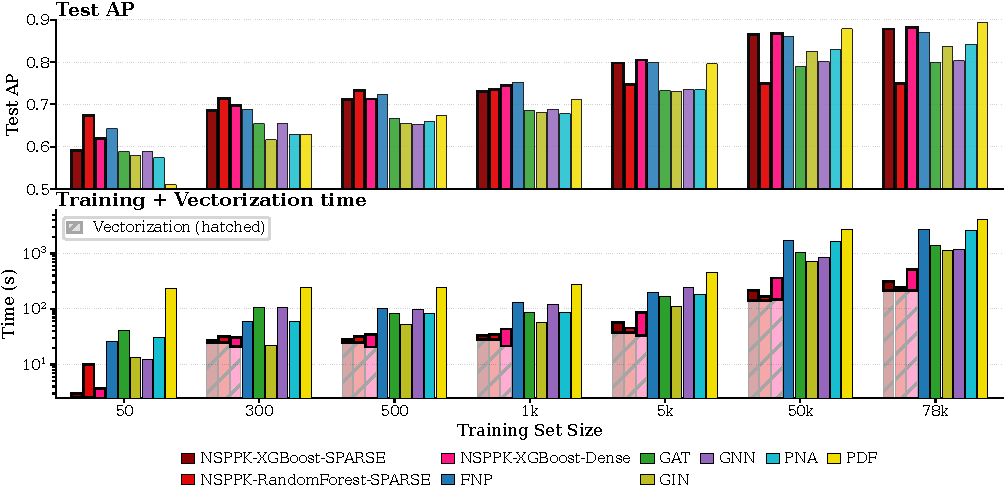
\includegraphics[width=.95\textwidth]{images/icml_compact_learning_curves.pdf}
  \caption{Learning curves on \texttt{ogbg-molpcba} (task~95).
  NSPPK (red) compared with neural baselines including GIN, GAT, PNA,
  PDF, and AttentiveFP (FNP).}
  \label{fig:large_experiment}
\end{figure*}
\section{Discussion and Limitations}
\label{sec:nsppk:discussion-limitations}

The results show that NSPPK can provide competitive graph-level features while
remaining deterministic and explicit. Its main advantage is that each active
dimension is tied to a hashed structural pattern involving anchor
neighbourhoods, connector paths, and attribute information. This supports
feature inspection: important coordinates can be traced back to the kinds of
substructures that produced them. The interpretation is therefore local to the
constructed feature map and the downstream model coefficients; it should not
be read as a complete causal explanation of a prediction.

The method also has practical limits. Feature extraction depends on the chosen
radii, anchor distances, and hash size. Larger values can capture richer
structure, but they also increase runtime and sparsity, especially on dense
graphs. Hashing makes the representation compact and efficient, but distinct
patterns may collide when the hash space is too small. The robustness analysis
therefore complements the classification results by testing whether the kernel
continues to produce meaningful similarities under controlled perturbations,
rather than assuming that sparsity alone is harmless.

Finally, NSPPK is a predefined representation. It does not learn which
substructures are useful before feature extraction; this choice is made by the
kernel design and its parameters. This can improve sample efficiency and
auditability, but it also means that task-specific adaptation is left to the
downstream learner. Hybrid approaches that use NSPPK features as inputs,
regularisers, or conditioning descriptors for neural graph models remain a
natural direction for future work.

\section{Conclusion}
\label{sec:Conclusion}

We introduced NSPPK, an explicit graph kernel that extends classical
neighbourhood-based representations through connector substructures and direct
integration of continuous node attributes, yielding sparse and interpretable
graph-level embeddings.  NSPPK belongs to the class of predefined,
data-independent methods while enriching their expressive power through richer
structural encoding.

NSPPK provides deterministic and training-free feature extraction, enabling
scalable graph learning with standard supervised models. Empirically, it
achieves the best average rank among the tested graph kernels and competitive
results against the neural baselines considered in this chapter, despite
avoiding representation learning or end-to-end optimisation. These results show
that carefully designed explicit representations can remain useful alongside
learned embeddings. Because NSPPK features correspond to hashed subgraph
patterns, predictive signals can be inspected by retrieving the structural
patterns associated with important feature coordinates.

Within the broader perspective of this thesis, NSPPK advances the
\emph{representation} component of graph learning. The next chapter complements
this direction by studying \emph{generation}, focusing on diffusion-based graph
models that learn probabilistic representations of graph distributions. While
NSPPK emphasises explicit structural encoding, diffusion models prioritise
flexible data-driven synthesis, together forming complementary approaches to
graph learning.

Future work includes hybrid kernel–neural models and extensions to dynamic or
temporal graphs.

\chapter{Graph-Conditioned Diffusion Generator}
\label{ch:generator}

\section{Chapter Introduction and Design Rationale}
\label{sec:generator:introduction}

Chapter~\ref{ch:theory} identified a central difficulty in graph generation:
diffusion and score-based generative models provide stable denoising objectives
\citep{ho2020ddpm,song2020score}, but graphs are discrete, sparse,
permutation-sensitive, and subject to structural constraints
\citep{you2018graphrnn,niu2020permutation,vignac2022digress}. This chapter
addresses that difficulty by introducing the
\emph{Graph-Conditioned Diffusion Generator} (GCDG), the generator used in this
thesis.

GCDG separates continuous diffusion from discrete graph construction. A
conditional diffusion process is applied to padded node-level feature matrices,
while node existence, labels, degrees, pairwise edges, and edge labels are
predicted by dedicated modules before a constraint-aware decoder selects the
final graph. Throughout this chapter,
\emph{diffusion} refers to the forward corruption and reverse noise-removal
process over node-level features, while \emph{denoising} refers to the learned
prediction task performed inside that process.

The conditioning signal is a fixed graph-level vector \(C\). In this thesis,
\(C\) is instantiated using the \gls{nsppk} feature map introduced in
Chapter~\ref{ch:nsppk}, so neighbourhood, shortest-path, connector, and
attribute information can guide generation. The architecture itself only
requires a fixed-dimensional graph descriptor; other explicit graph descriptors,
graph kernels, or learned graph-level embeddings could therefore be substituted
\citep{costa2010fast,neumann2016propagation,borgwardt2020graphkernels,
hamilton2017graphsage,zhang2018endtoend,dwivedi2021graph}.

The setting considered here is graph-level-descriptor-to-graph generation. This
differs from unconditional generation, class-conditional generation, and
property-conditional generation, where the condition is often a class label or a
small set of scalar targets. It also differs from graph autoencoders and
variational graph autoencoders, which encode a specific input graph into a
sample-specific latent code before decoding it
\citep{kipf2016vgae,simonovsky2018graphvae}. GCDG receives only \(C\): when the
condition is computed from a reference graph, the target is not to reconstruct
that graph exactly, but to generate a graph that preserves information encoded
by the condition.
\begin{figure}[H]
    \centering
    \makebox[\textwidth][c]{%
    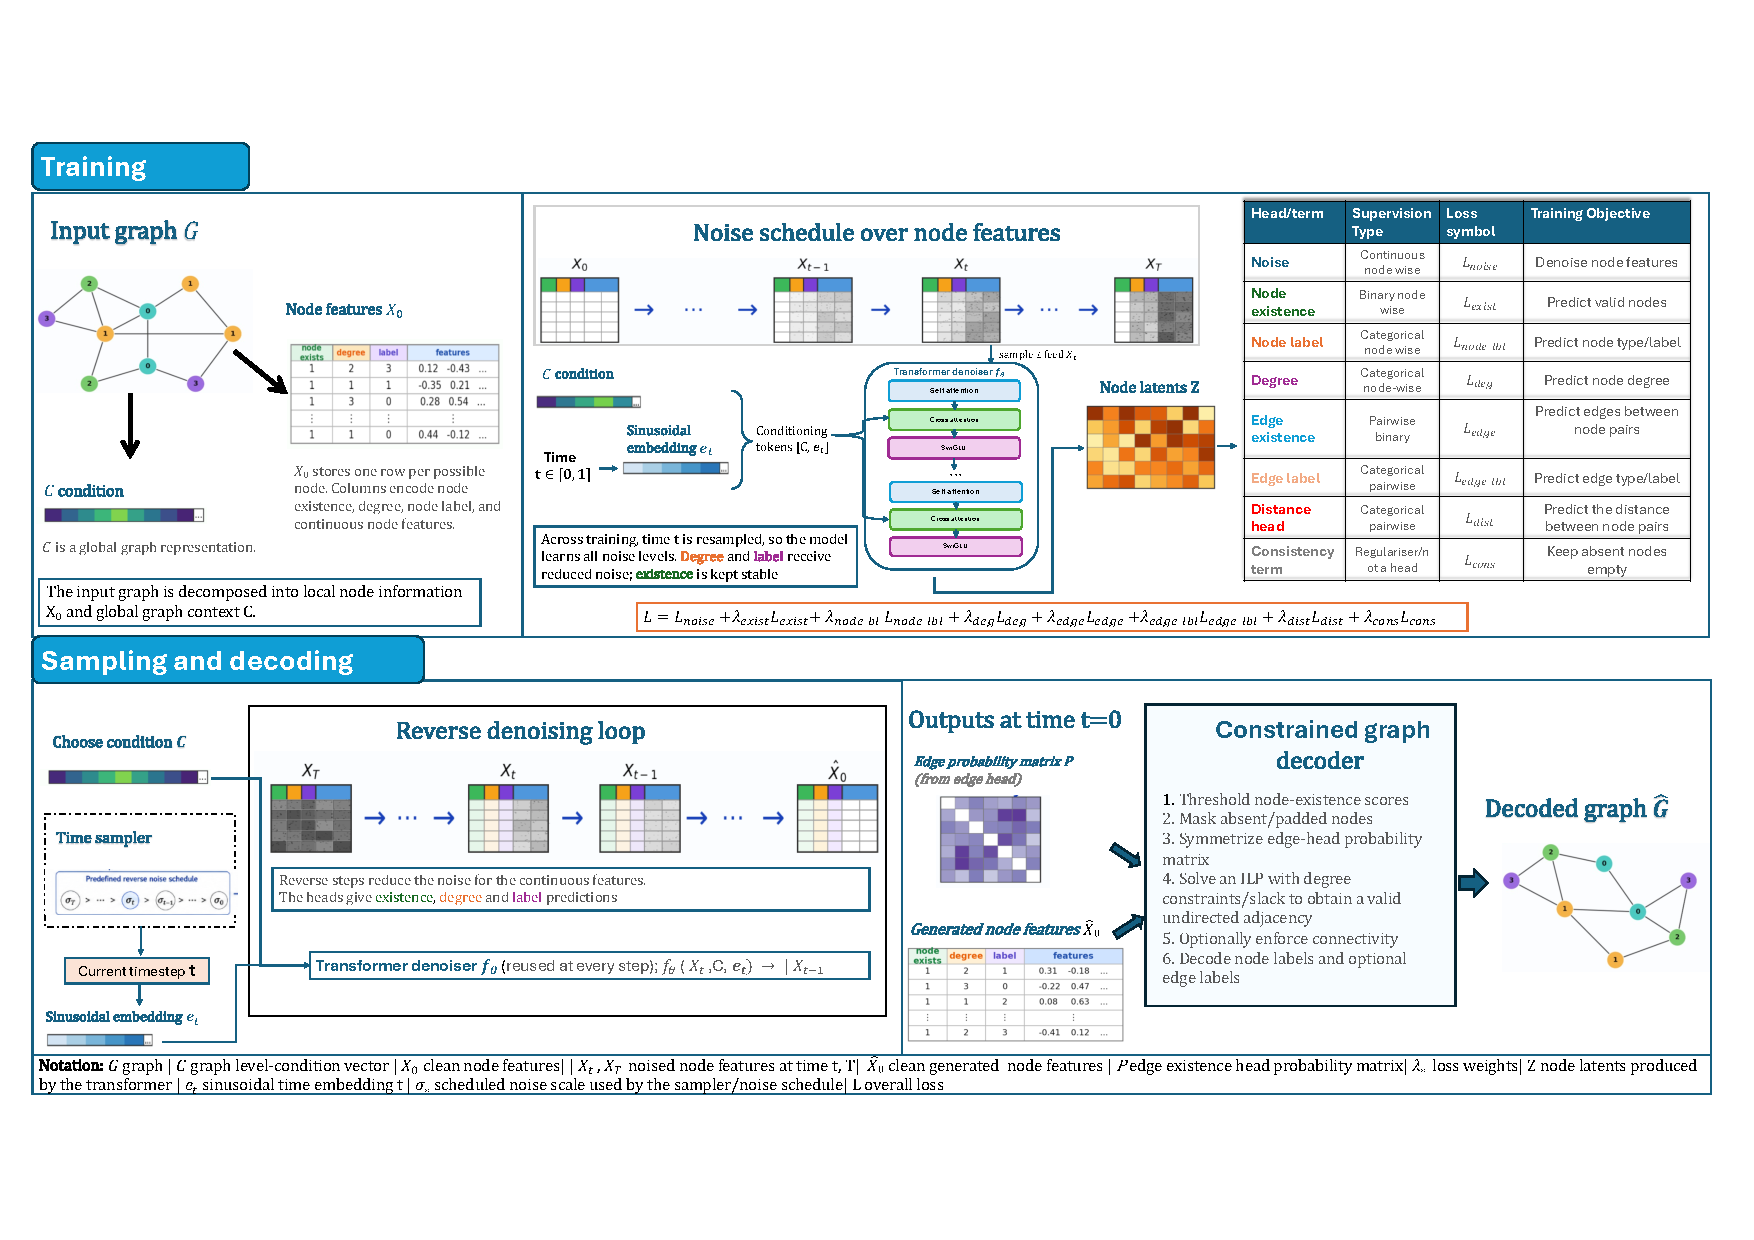
\includegraphics[
        width=1.25\textwidth,
        height=0.60\textheight,
        keepaspectratio,
        trim=0cm 2cm 0cm 2cm,
        clip
    ]{images/diffusion/pipeine_generator.pdf}
    }
    \caption{
    Overview of GCDG. The input graph is encoded into a padded node-level
    representation \(X_0\) and a graph-level condition vector \(C\). During
    training, a time \(t\) is sampled and noise is added to \(X_0\) according to
    a feature-wise schedule, producing \(X_t\). The conditional transformer
    receives \(X_t\), \(C\), and the time embedding \(e_t\), and produces
    node-level latents used by node-wise and pairwise prediction modules. At
    sampling time, a reverse noise schedule is followed from \(X_T\) to
    \(\hat X_0\), reusing the same denoising model at each step. The generated
    node representation and edge probability matrix are decoded into a graph by
    the constrained decoder.
    }
    \label{fig:generator:overview}
\end{figure}

The central contribution of this chapter is therefore the
graph-level-to-node-and-edge-level formulation. The model must translate a global structural
descriptor into the quantities needed to build a discrete graph: which nodes
exist, which labels and degrees they have, and which pairwise edges should be
selected. This is also distinct from direct graph diffusion models such as
DiGress, where the reverse process operates on categorical node and edge states
\citep{vignac2022digress}. In GCDG, the diffusion process acts on node-level
features, and graph topology is constructed through pairwise prediction and
constraint-aware decoding.

The rest of this chapter develops this staged generator in detail. It defines
the node-level representation, graph-level condition, diffusion architecture,
training objective, sampling procedure, and constraint-aware graph decoder.


\section{Method Overview and Representations}
\label{sec:generator:method-overview}


\subsection{Node-Level Feature Representation and Graph-Level Conditions}
\label{sec:generator:representation}

Let
\[
    G=(V,E,\tau_V,\tau_E)
\]
denote a finite, simple, undirected, discretely labelled graph, where
\[
    V=\{v_1,\ldots,v_n\},
    \qquad
    n=|V|,
\]
is the set of nodes and \(E\) is the set of edges. The functions
\[
    \tau_V:V\to\mathcal{T}_V
    \qquad\text{and}\qquad
    \tau_E:E\to\mathcal{T}_E
\]
assign discrete labels to nodes and edges, respectively. Let
\[
    K_V = |\mathcal{T}_V|
\]
denote the number of node-label classes.
In the terminology of Chapter~\ref{ch:theory}, these labels are categorical
node and edge attributes. The notation \(\tau_V,\tau_E\) is used deliberately
to avoid overloading the supervised-learning label space \(\mathcal{Y}\) or
the layer index \(\ell\) from the notation list.

The generator represents each graph at two complementary levels. At the graph
level, the default conditioning representation is obtained using the
\gls{nsppk} feature map introduced in Chapter~\ref{ch:nsppk}:

\[
    C
    =
    \phi_{\mathrm{NSPPK}}^{\mathrm{graph}}(G)
    \in
    \mathbb{R}^{d_C},
\]

where \(d_C\) is the dimension of the graph-condition vector. The vector \(C\)
summarises labelled neighbourhood patterns and broader structural relations in
\(G\), and is used as the graph-level description that conditions the denoising
process. This follows the graph-kernel view in which a graph is represented by
an explicit feature map \(\phi(G)\)
\citep{costa2010fast,borgwardt2005shortest,neumann2016propagation}. When the
resulting feature vector is high-dimensional, it may be compressed using a
dimensionality-reduction transformation, such as truncated \gls{svd}, fitted on
the training graphs. Once fitted, this transformation is held fixed: the same
projection is applied unchanged to training graphs, held-out condition graphs,
and generated graphs that are re-encoded for analysis.
The resulting graph-level condition vectors are also scaled using training-set
statistics. This scaling is fitted only on the training conditions and then
kept fixed, so held-out conditions and generated graphs are represented in the
same coordinate system.

Although \gls{nsppk} is the default condition encoder used in this thesis, the
generator architecture is not restricted to this particular feature map. More
generally, it requires a real-valued graph-level condition
\[
    \phi:\mathcal{G}\to\mathbb{R}^{d_C},
\]
where \(\mathcal{G}\) denotes the set of graphs considered in the task. Thus,
alternative explicit graph descriptors or learned graph-level embeddings can
replace \(\phi_{\mathrm{NSPPK}}^{\mathrm{graph}}\), provided that they produce a
compatible conditioning vector \(C\). Examples include learned graph
representations from graph neural networks or graph Transformers
\citep{hamilton2017graphsage,zhang2018endtoend,dwivedi2021graph}.

At the node level, the \gls{nsppk} node encoder produces a structural feature
vector for each node \(v_i\in V\):

\[
    r_i
    =
    \phi_{\mathrm{NSPPK}}^{\mathrm{node}}(v_i;G)
    \in
    \mathbb{R}^{d_r},
\]
Let $\mathcal{F}_i(G)$ denote the set of NSPPK feature occurrences assigned to
node $v_i$. The node-level structural representation is defined as
\[
r_i
=
\sum_{\xi\in\mathcal{F}_i(G)}
e_{h(\xi)}.
\]
where $h(\xi)$ is the hash bucket assigned to feature occurrence $\xi$ and
$e_{h(\xi)}$ is the corresponding standard basis vector.  At
a high level, \(r_i\) describes the labelled local structural context of node
\(v_i\), including the root-node label, labels of neighbouring nodes and
incident edges, rooted neighbourhood patterns over selected radii, and
relations between nearby neighbourhoods connected through short graph paths.
The representation is sparse and hash-based, so nodes with similar labelled
local structure activate similar feature dimensions.

The generator represents graphs with at most \(N_{\max}\) nodes, where
\(N_{\max}\) is fixed for a dataset or experimental setting. For each possible
node row \(i\in\{1,\ldots,N_{\max}\}\), the row of the node feature matrix is

\[
x_i
=
\left[
m_i;\,
g_i;\,
q_i;\,
r_i
\right]
\in\mathbb{R}^{d_{\mathrm{feat}}},
\]

Here $m_i\in\{0,1\}$ is the node-existence indicator and
\[
g_i=\deg(v_i)
\]
is the degree of node $v_i$ when row $i$ represents a real node. Before being
supplied to the denoising network, the degree coordinate is transformed using
the fitted node-feature scaler. For the auxiliary degree-prediction task, the
unscaled integer degree is treated as a categorical target in
\[
\{0,\ldots,D_{\max}\},
\]
where $D_{\max}$ is the maximum degree supported by the fitted model. The
degree-prediction head therefore has $D_{\max}+1$ output classes.

If degrees are clipped or grouped, the corresponding mapping is
defined by the experimental configuration.

\[
    q_i
    =
    \left[
        q_i^{(1)},\ldots,q_i^{(K_V)}
    \right]
    \in
    \{0,1\}^{K_V}
\]
is the one-hot encoding of the node label \(\tau_V(v_i)\). The final component
\(r_i\) contains the node-level \gls{nsppk} structural features. The
node-feature dimension is therefore
\[
    d_{\mathrm{feat}} = 2 + K_V + d_r.
\]
In the rest of this chapter, a \emph{feature component} refers to one scalar
entry or one contiguous block in this row vector: the existence component
\(m_i\), the degree component \(g_i\), the node-label one-hot block \(q_i\), or
the continuous structural representation \(r_i\).

The label vocabulary is learned from the training dataset and stored by the
encoder. Numeric labels, symbolic role labels, and molecular atom symbols are
all treated as unordered categorical classes. The decoder uses the stored
mapping to convert generated class indices back to the original node labels.
Since labels are discrete, the model predicts node-label logits and trains them
with cross-entropy over existing nodes; they are not reconstructed by scalar
regression.

Let \(N_{\max}\) denote the fixed row budget used for padding, chosen to cover
the largest graphs considered in a given experiment. The feature vectors are
stacked and padded to form the clean node feature matrix
\[
X_0
=
\begin{bmatrix}
x_1^\top\\
\vdots\\
x_n^\top\\
x_{n+1}^\top\\
\vdots\\
x_{N_{\max}}^\top
\end{bmatrix}
\in
\mathbb{R}^{N_{\max}\times d_{\mathrm{feat}}}.
\]


For a graph containing $n<N_{\max}$ nodes, rows $i>n$ represent padding rather
than real graph nodes. In these rows, $m_i=0$, while the remaining feature
components are assigned fixed padding values. Loss terms for degree, node
label, continuous reconstruction, and supervised node pairs use the existence
mask to exclude non-existent rows.

In the current implementation, padded rows remain present as transformer
tokens and are not removed by an attention padding mask. They may therefore
participate in intermediate self-attention computations, although they are
excluded from the masked training targets and from final graph decoding. This
fixed-row representation is retained consistently during training and
sampling.


Before the denoising model is trained, the continuous coordinates of the node
feature matrix are placed on a common numerical scale. The scaler is fitted on
real node rows from the training graphs, after any optional dimensionality
reduction of the structural feature block, and is then reused for validation
graphs, held-out reference graphs, and generated samples. Padding rows are not
used to fit this scaler. The node-existence component is kept as a binary indicator, rather
than being rescaled, because it is the mask that distinguishes real node rows
from padding rows. For notational simplicity, the equations below use \(X_0\)
for this internally scaled clean node feature matrix.

Because graph nodes do not have a canonical order, the row order in \(X_0\) is
an implementation choice rather than an intrinsic graph property. Two node
feature matrices that differ only by a simultaneous permutation of their rows
can represent the same labelled graph. The generator therefore uses two
training-time devices to reduce sensitivity to arbitrary row order. First, node
rows can be randomly permuted during training. Second, the clean-\(X_0\)
reconstruction loss can be evaluated after matching predicted rows to target
rows.

The matching step is a linear assignment problem. Given a predicted clean node
feature matrix \(\hat X_0\) and a target matrix \(X_0\), define a pairwise cost
between predicted row \(i\) and target row \(j\),
\[
c_{ij}
=
\left\|
B_{\mathrm{match}}
\odot
(\hat{x}_{0,i}-x_{0,j})
\right\|_2^2.
\]
where \(B_{\mathrm{match}}\) selects the continuous structural coordinates used
for matching. The matched target order is obtained by finding the permutation
\[
    \pi^\star
    =
    \arg\min_{\pi\in S_{N_{\max}}}
    \sum_{i=1}^{N_{\max}} c_{i,\pi(i)} .
\]
This is the classical assignment problem, solved in the implementation using
the Hungarian algorithm \citep{kuhn1955hungarian,munkres1957algorithms}. The
algorithm can be understood as finding the minimum-cost one-to-one pairing
between the predicted rows and the target rows. In this generator, the matching
cost deliberately excludes the existence, degree, and node-label components, so
the categorical prediction losses cannot choose an artificially favourable
alignment. The assignment itself is not a learned neural module and is not part
of sampling. It is a training alignment step: after \(\pi^\star\) is selected,
the usual losses compare the prediction with the permuted target rows.
The assignment is performed over the complete padded row set. Because the
existence component is excluded from the matching cost, the assignment does
not explicitly prevent a predicted real-node row from being matched to a
padded target row. The separate existence and categorical losses provide the
corresponding supervision.
The node feature matrix captures node existence, degree, node labels, and
node-level structural context. It does not directly specify the final adjacency
matrix.
Instead, edge existence and, when applicable, the discrete edge label
\[
    \tau_E(\{v_i,v_j\})
\]
are estimated separately for candidate node pairs by the pairwise prediction
module. The graph decoder then combines the generated node features and
pairwise edge predictions to construct the final discrete graph.

\section{Forward Diffusion and Corruption Process}
\label{sec:generator:forward}

During training, the clean node feature matrix \(X_0\) is corrupted at a
randomly sampled noise level. A time value

\[
    t \sim \mathcal{U}(0,1)
\]
is mapped to a noise scale

\[
    \sigma(t) = \sigma_{\min}
    + t(\sigma_{\max}-\sigma_{\min}).
\]
Gaussian noise is then added feature-wise:

\[
    X_t = X_0 + \Gamma(t) \odot \varepsilon,
    \qquad
    \varepsilon \sim \mathcal{N}(0,I),
\]
where \(\Gamma(t)\) contains the per-feature noise scales and \(\odot\) denotes
element-wise multiplication. This corruption process is not used in the same
way for every feature component. Continuous structural features are learned through a
denoising task, whereas node existence, degree class, and node-label attributes
are treated as supervised classification tasks. The model therefore does not ask
a single continuous reconstruction objective to recover all discrete quantities.
Instead, the training objective combines a continuous denoising loss for
real-valued feature dimensions with separate binary or categorical losses for the
discrete node attributes. The architectural modules that implement these
supervised losses are introduced in the next section.

For the categorical feature blocks, Gaussian perturbation is not the only
meaningful way to define a noisy input. A node label, for example, is not a
number whose value should be slightly increased or decreased; it is a class
membership. For this reason, the categorical part of the forward process can
also be defined as a discrete corruption task. The model is shown a corrupted
degree or node-label class at noise level \(t\), and the supervised target is
the original clean class from \(X_0\). In a random-replacement corruption, the
clean class is replaced by another class with probability increasing in \(t\).
In an absorbing corruption, the clean class is replaced by a special unknown or
masked class. These operators play the same conceptual role as noise in a
discrete diffusion process: they gradually remove categorical information while
leaving a well-defined classification target for the reverse model.

\section{Conditional Denoising Architecture}
\label{sec:generator:architecture}

The denoising network is implemented as a transformer over the node-feature
matrix. This choice follows the use of
attention mechanisms in graph representation learning and graph generation,
where interactions between many possible node pairs must be represented without
committing to a sequential node ordering
\citep{vaswani2017attention,dwivedi2021graph,ying2021transformers,
rampavsek2022recipe,vignac2022digress}. In this chapter, each row of
\(X_t\) is treated as a node token. Because the same projections are applied to
all node rows and no order-specific positional encoding is used, the
transformer is equivariant to permutations of the complete padded row set:
permuting the rows of \(X_t\) permutes the resulting node latents in the same
way. The current
implementation does not apply an attention padding mask, so padded rows remain
part of the intermediate self-attention computation.

The noisy node feature matrix is first normalised and projected to
latent tokens:

\[
    R^{(0)} = W_X \operatorname{LN}(X_t) + b_X.
\]

Here \(\operatorname{LN}\) denotes layer normalisation, while \(W_X\) and
\(b_X\) are learned projection parameters that map each normalised node row
into the latent dimension.

A sinusoidal embedding of the noise level produces a time token \(e_t\). Such
embeddings are standard in transformer architectures and diffusion models
because they map a scalar position or noise level to a multi-frequency vector
that can be used by a shared neural network across many steps
\citep{vaswani2017attention,ho2020ddpm}. The graph condition is projected to a
second memory token:

\[
    c = W_C C + b_C.
\]

Here \(W_C\) and \(b_C\) are learned parameters for projecting the graph-level
condition into the same latent dimension as the node tokens.

The transformer therefore receives node tokens \(R^{(0)}\) and attends to the
memory sequence

\[
    \mathcal{M} = [e_t, c].
\]

Each block applies self-attention over node tokens, cross-attention to the time
and condition memory tokens, and a feed-forward transformation. Self-attention
lets each node representation depend on the other currently generated node
representations, which is necessary because node roles, degrees, and labels are
not independent. Cross-attention is used for the global variables \(t\) and
\(C\): every node token can query the same noise-level and graph-level
condition information, while the condition remains a graph-level object rather
than being treated as an additional node. The final node latents are

\[
    Z = F_\theta(X_t, C, t) \in
    \mathbb{R}^{N_{\max} \times d_Z}.
\]

Here \(F_\theta\) denotes the learned conditional transformer map and \(d_Z\)
is the node-latent dimension.

The model then solves several supervised prediction tasks from \(Z\). A
continuous prediction module estimates the Gaussian noise
\(\hat{\varepsilon}\) for non-discrete feature dimensions. A binary classifier
predicts node existence. Two categorical classifiers predict the degree class
and the node-label class. Edges are not represented as cross-attention tokens;
instead, edge existence is predicted pairwise from the two endpoint latents.

Let $z_i\in\mathbb{R}^{d_Z}$ denote the $i$th row of $Z$. For an ordered
candidate pair $(i,j)$, the edge-existence head computes the biaffine logit
\[
s_{ij}^{\mathrm{edge}}
=
z_i^{\top}B_{\mathrm{edge}}z_j
+
a_{\mathrm{edge}}^{\top}[z_i;z_j]
+
b_{\mathrm{edge}},
\]
followed by
\[
p_{ij}^{\mathrm{edge}}
=
\operatorname{sigmoid}
\left(
s_{ij}^{\mathrm{edge}}
\right).
\]
Here
\[
B_{\mathrm{edge}}\in\mathbb{R}^{d_Z\times d_Z},
\qquad
a_{\mathrm{edge}}\in\mathbb{R}^{2d_Z},
\qquad
b_{\mathrm{edge}}\in\mathbb{R}
\]
are learned parameters, and $[z_i;z_j]$ denotes vector concatenation.

The raw biaffine score need not be invariant to exchanging $i$ and $j$.
For undirected generation, the implementation forms a dense probability
matrix, averages it with its transpose, and sets its diagonal to zero before
using it as the undirected edge-probability matrix.

 
 When edge labels are available, a
second pairwise classifier predicts a distribution
\(p^{\tau_E}_{ij}\in\Delta^{|\mathcal{T}_E|-1}\) over the edge-label classes
for each supervised pair, where \(\Delta^{K-1}\) denotes the probability
simplex over \(K\) classes. When distance supervision is enabled, another
pairwise classifier predicts a distribution
\(p^{\mathrm{dist}}_{ij}\) over binned graph distances between node pairs. These
pairwise prediction tasks provide additional supervision for the node latents
during training, while \(p^{\mathrm{edge}}_{ij}\) is also passed to the graph
decoder.

\subsection{Joint Edge State}
\label{sec:generator:joint-edge-state}

The base generator predicts edges from the final node latents and then passes
the resulting probabilities to the decoder. An optional joint edge-state variant makes edge information part of the reverse
diffusion trajectory itself. The purpose is to let
intermediate node representations depend not only on the current node feature
matrix \(X_t\), but also on a provisional graph structure.

This idea is inspired by discrete graph diffusion models such as DiGress, where
the noisy state at each reverse step contains both node and edge information
\citep{vignac2022digress}. The present model does not adopt full discrete edge
diffusion: the adjacency matrix is still decoded at the end by the constrained
graph decoder. Instead, it borrows the principle that the reverse model should
be allowed to condition on an evolving noisy graph structure while it denoises
node-level representations.
The mechanism is therefore different from DiGress even when it is enabled. In
DiGress, the reverse model predicts transitions for discrete node and edge
states. Here, the edge state is not the main generated object. It is an
auxiliary structural signal injected into the node-latent computation, so that
the denoiser can update \(Z_t\) using both the noisy node feature matrix
\(X_t\) and the provisional adjacency \(A_t^{\mathrm{state}}\). The final
adjacency is still selected later by the graph decoder.

Let \(A_0\in\{0,1\}^{N_{\max}\times N_{\max}}\) denote the padded clean
adjacency matrix. During training, an edge-state matrix
\(A_t^{\mathrm{state}}\) is obtained by corrupting \(A_0\): true edges may be
deleted and false edges may be inserted, with corruption probabilities
increasing with the noise level. This creates a noisy structural context for
the denoiser. To make explicit how the provisional adjacency enters the latent
representation, write
\[
H_t
=
\begin{bmatrix}
h_{t,1}^{\top}\\
\vdots\\
h_{t,N_{\max}}^{\top}
\end{bmatrix}
\in
\mathbb{R}^{N_{\max}\times d_Z}
\]
for the node latents produced by the transformer before the edge-state update.
The edge state is not concatenated as an additional feature column. Instead,
it is used as a soft adjacency matrix that forms a neighbourhood summary for
each node.


\[
    \bar h^{\mathrm{edge}}_{t,i}
    =
    \frac{
        \sum_{j=1}^{N_{\max}}
        A^{\mathrm{state}}_{t,ij} h_{t,j}
    }{
        \max\left(1,\sum_{j=1}^{N_{\max}}
        A^{\mathrm{state}}_{t,ij}\right)
    }.
\]

The node latent is then refined by a residual message-passing update,

\[
    z_{t,i}
    =
    h_{t,i}
    +
    \phi_{\mathrm{edge}}
    \left(
        \left[
        \operatorname{LN}(h_{t,i});
        \bar h^{\mathrm{edge}}_{t,i}
        \right]
    \right),
\]

where \(\phi_{\mathrm{edge}}\) is a learned multilayer perceptron and
\([\,\cdot\,;\,\cdot\,]\) denotes concatenation. Thus the final latent
\(z_{t,i}\) contains information from the node's own noisy row, the graph-level
condition and time embedding, and a weighted summary of the nodes that are
currently likely to be adjacent to it. Let
\(\operatorname{EdgeMP}_\theta\) denote this learned edge-state
message-passing operator, parameterised by \(\phi_{\mathrm{edge}}\). In matrix
form, this optional refinement can be written as

\[
    Z_t = \operatorname{EdgeMP}_\theta(H_t,A_t^{\mathrm{state}}).
\]

The node representation is therefore conditioned on the provisional edge
structure as well as on \(X_t\), \(C\), and \(t\).

The training-time corruption can be read as an edge analogue of the
node-feature diffusion process. Starting from the clean adjacency \(A_0\), the
model removes some true edges and inserts some false edges to obtain
\(A_t^{\mathrm{state}}\). At small noise levels, this state remains close to
the true graph; at large noise levels, it becomes a rougher provisional
structure. The denoiser must therefore learn to use edge information when it is
helpful while remaining robust to structural mistakes in the provisional graph.

During generation, \(A_T^{\mathrm{state}}\) is initialised as a sparse symmetric
matrix. At each reverse step, the edge-existence classifier predicts a matrix
of edge probabilities from the current node latents. The running edge state is
then updated by momentum:

\[
    A_{t-1}^{\mathrm{state}}
    =
    \mu A_t^{\mathrm{state}} +
    (1-\mu) P_\theta^{\mathrm{edge}}(Z_t),
\]

where \(0\leq\mu\leq1\) controls how much of the previous edge state is retained
and \(P_\theta^{\mathrm{edge}}(Z_t)\in[0,1]^{N_{\max}\times N_{\max}}\) is the
matrix with entries \(p^{\mathrm{edge}}_{ij}\). At low noise levels, this state
may be thresholded to obtain a sharper provisional adjacency. In this variant,
edge information is not only a final output of the pairwise classifier; it is a
state variable that can influence subsequent reverse diffusion steps.
Both the initial edge state and the dense predicted edge-probability matrix are
constructed symmetrically with zero diagonal. Their convex combination
therefore remains symmetric and excludes self-loops. At sufficiently low noise
levels, the resulting state may be thresholded.


\begin{figure}[H]
    \centering
    \small
    \[
    \begin{aligned}
    A_0
    &\xrightarrow{\text{delete true edges / add false edges}}
    A_t^{\mathrm{state}},
    \\
    (X_t,A_t^{\mathrm{state}},C,t)
    &\xrightarrow{\text{transformer}}
    H_t,
    \\
    (H_t,A_t^{\mathrm{state}})
    &\xrightarrow{\text{edge-state message passing}}
    Z_t,
    \\
    Z_t
    &\xrightarrow{\text{edge classifier}}
    P_\theta^{\mathrm{edge}}(Z_t),
    \\
    A_{t-1}^{\mathrm{state}}
    &=
    \mu A_t^{\mathrm{state}}
    +(1-\mu)P_\theta^{\mathrm{edge}}(Z_t).
    \end{aligned}
    \]
    \caption{
    Joint edge-state mechanism. During training, the clean adjacency \(A_0\) is
    corrupted into a noisy edge state \(A_t^{\mathrm{state}}\). During sampling,
    the current edge state is fed into the denoiser, updated using the predicted
    edge-probability matrix, and reused at the next reverse step. The final
    graph is still obtained by constrained decoding rather than by directly
    sampling all edges from this state.
    }
    \label{fig:generator:joint-edge-state}
\end{figure}

\subsection{Optional Dynamic Molecular Features}
\label{sec:generator:dynamic-molecular}

The generator above is dataset-agnostic: node labels are treated as categorical
attributes, not as chemical atom types. For molecular experiments, we also
consider a chemistry-aware extension that gives the denoiser access to simple
state-dependent molecular summaries. This is motivated by the fact that
chemical validity depends on relationships between atom identity and incident
bond order, for example whether the current provisional structure exceeds the
allowed valency of an atom.

At a diffusion step \(t\), let \(M_t^{\mathrm{mol}}\in
\mathbb{R}^{N_{\max}\times 5}\) denote a molecular state matrix computed from
the current atom-label probabilities and the current edge state. Its five
node-wise features are the current valency, the expected allowed valency, the
valence deficit, the expected atom weight, and a graph-level molecular-weight
summary copied to each node row. This matrix is not a learned classifier
output; it is a deterministic summary of the current generated molecular state.
It is projected into the latent dimension and added to the node tokens:

\[
    R^{(0)}
    \leftarrow
    R^{(0)}
    + \lambda_{\mathrm{mol}} W_{\mathrm{mol}} M_t^{\mathrm{mol}}.
\]

Here \(W_{\mathrm{mol}}\) is a learned projection and
\(\lambda_{\mathrm{mol}}\) controls the strength of the molecular-state
injection. This extension is not part of the dataset-agnostic core generator.
It is reported separately as a chemistry-aware ablation, because it supplies
domain knowledge that is not available for arbitrary graph datasets.

\section{Training Objective}
\label{sec:generator:objective}

The model is trained using a weighted combination of continuous denoising,
categorical node supervision, edge supervision, and optional auxiliary losses.
The continuous denoising loss is applied only to real node rows and to feature
dimensions intended to be denoised continuously:

\[
    \mathcal{L}_{\varepsilon}
    =
    \frac{
        \sum_i m_i
        \left\|
            B_{\mathrm{cont}}
            \odot
            (\hat{\varepsilon}_i - \varepsilon_i)
        \right\|_2^2
    }{
        \sum_i m_i + \eta_{\mathrm{num}}
    }.
\]

Here \(m_i\in\{0,1\}\) indicates whether row \(i\) corresponds to a real node
rather than padding, \(B_{\mathrm{cont}}\) masks out feature dimensions handled
by separate categorical heads, such as node existence, degree, and label, and
\(\eta_{\mathrm{num}}>0\) is a small numerical stabiliser. The terms
\(\varepsilon_i\) and \(\hat{\varepsilon}_i\) denote the sampled Gaussian noise
and the predicted noise for row \(i\), respectively. The clean-\(X_0\) estimate is

\[
    \hat{X}_0 = X_t - \Gamma(t)\odot \hat{\varepsilon}.
\]

An optional direct clean-\(X_0\) reconstruction loss can be used to anchor the
reverse diffusion process:

\[
    \mathcal{L}_{x_0}
    =
    \frac{
        \sum_i m_i
        \left\|
            B_{\mathrm{cont}}
            \odot
            (\hat{x}_{0,i} - x_{0,i})
        \right\|_2^2
    }{
        \sum_i m_i + \eta_{\mathrm{num}}
    }.
\]

Node existence is trained using binary cross-entropy, where \(m\) is the true
existence mask and \(\hat m\) denotes the predicted existence logits:

\[
    \mathcal{L}_{\mathrm{exist}}
    =
    \operatorname{BCEWithLogits}(\hat{m}, m).
\]

Here \(\operatorname{BCEWithLogits}\) denotes binary cross-entropy applied
directly to logits.

Degree and node-label attributes are trained using masked cross-entropy over
existing node rows. Let \(g_i\) and \(q_i\) denote the true degree and
node-label classes, and let \(\hat g_i\) and \(\hat q_i\) denote the
corresponding predicted logits.

When edge supervision is enabled, sampled node pairs are used to train the
biaffine edge head. Here \(A_{ij}\) is the true binary edge indicator and
\(\hat A_{ij}\) denotes the predicted edge logit:

Let $\mathcal{P}_{\mathrm{sup}}$ denote the set of supervised unordered node
pairs. Then
\[
\mathcal{L}_{\mathrm{edge}}
=
\frac{1}{|\mathcal{P}_{\mathrm{sup}}|}
\sum_{\{i,j\}\in\mathcal{P}_{\mathrm{sup}}}
w_{ij}\,
\operatorname{BCEWithLogits}
\left(
s^{\mathrm{edge}}_{ij},
A_{ij}
\right),
\]
where $w_{ij}$ optionally balances edge and non-edge examples. Pairs involving
padded rows are excluded.
Both categorical losses are evaluated only over real node rows:
\[
\mathcal{L}_{\mathrm{deg}}
=
\frac{1}{\sum_i m_i}
\sum_i
m_i\,
\operatorname{CE}(\hat g_i,g_i),
\]
and
\[
\mathcal{L}_{\tau_V}
=
\frac{1}{\sum_i m_i}
\sum_i
m_i\,
\operatorname{CE}(\hat q_i,q_i).
\]
If edge labels are present, the edge-label term is a categorical
cross-entropy over supervised node pairs and is denoted
\(\mathcal{L}_{\tau_E}\). Optional distance supervision gives
\(\mathcal{L}_{\mathrm{dist}}\). The consistency term
\(\mathcal{L}_{\mathrm{cons}}\) discourages non-existent padded rows from
carrying non-zero continuous information. The optional condition-to-\(X_0\)
head predicts a clean node feature matrix directly from the condition, giving
an auxiliary loss \(\mathcal{L}_{C\rightarrow X_0}\). This head can also be used
as a sampling prior, but it is not required for the main generator. An optional
clean-edge term \(\mathcal{L}_{\mathrm{clean\text{-}edge}}\) applies the same
edge-existence supervision to latents evaluated at an approximately clean noise
level.

The full objective can therefore be written as

\[
\begin{aligned}
    \mathcal{L}
    ={}&
    \lambda_{\varepsilon}\mathcal{L}_{\varepsilon}
    + \lambda_{x_0}\mathcal{L}_{x_0}
    + \lambda_{C\rightarrow X_0}\mathcal{L}_{C\rightarrow X_0}
    + \lambda_{\mathrm{exist}}\mathcal{L}_{\mathrm{exist}}
    + \lambda_{\mathrm{deg}}\mathcal{L}_{\mathrm{deg}}
    + \lambda_{\tau_V}\mathcal{L}_{\tau_V}  \\
    &+
    \lambda_{\mathrm{edge}}\mathcal{L}_{\mathrm{edge}}
    + \lambda_{\mathrm{clean\text{-}edge}}\mathcal{L}_{\mathrm{clean\text{-}edge}}
    + \lambda_{\tau_E}\mathcal{L}_{\tau_E}
    + \lambda_{\mathrm{dist}}\mathcal{L}_{\mathrm{dist}}
    + \lambda_{\mathrm{cons}}\mathcal{L}_{\mathrm{cons}}.
\end{aligned}
\]

Each coefficient \(\lambda_{\bullet}\geq 0\) weights the loss term with the
corresponding subscript. For example, \(\lambda_{\mathrm{dist}}\) weights the
distance-classification loss and \(\lambda_{\tau_E}\) weights the edge-label
loss. Terms whose corresponding head or supervision source is absent are set to
zero and omitted from training. When the joint edge-state variant is enabled,
\(\lambda_{\mathrm{edge}}\) also weights the dense edge-state reconstruction
term. The implementation additionally applies inverse-noise weights to the node
and pairwise classification losses, so lower-noise examples contribute more
strongly when the target discrete structure is less corrupted.

\section{Reverse Diffusion and Sampling Process}
\label{sec:generator:sampling}

The reverse diffusion process defines conditional generation from a graph-level
description \(C\). The condition may be drawn from an empirical set of
conditions, such as held-out graphs, or chosen to represent a desired
target property. Given \(C\), generation starts from an uncommitted padded node
feature matrix \(X_T\). Its continuous feature dimensions are initialised with
Gaussian noise, while the discrete feature blocks are initialised close to
uninformative states: uncertain existence, broad degree support, and an
approximately uniform node-label distribution. In ablations that include a
direct condition-to-\(X_0\) prior, this initial state can be biased toward the
prior prediction; otherwise, the reverse diffusion process begins from the
neutral noisy state.

The reverse diffusion trajectory follows a decreasing sequence of noise levels
\(\sigma_T > \cdots > \sigma_0\). At each step, the denoiser estimates the
noise component that should be removed from the current node feature matrix.
The continuous feature dimensions are then advanced using an Euler predictor
followed by a Heun correction:

\[
    X_{\mathrm{pred}}
    =
    X_t - (\sigma_t-\sigma_{t-1})\hat{\varepsilon}_t,
\]

\[
    X_{t-1}
    =
    X_t
    -
    \frac{1}{2}(\sigma_t-\sigma_{t-1})
    (\hat{\varepsilon}_t+\hat{\varepsilon}_{t-1}).
\]

The learned reverse vector field is applied only to continuous feature dimensions.
Discrete node attributes are recovered through their supervised prediction
modules. Thus, after the final reverse diffusion step, node existence is obtained by
thresholding the existence probability, the degree class is obtained by
categorical projection, and the node label is obtained from the node-label
distribution. If the joint edge-state variant is used, the provisional edge
state is updated throughout the reverse diffusion trajectory; otherwise, edge
probabilities are computed from the final node latents before graph decoding.

\begin{algorithm}[H]
\caption{Reverse diffusion sampling of the node feature matrix}
\label{alg:generator:sampling}
\begin{algorithmic}[1]
\Require Graph-level condition \(C\), noise schedule
\(\sigma_T,\ldots,\sigma_0\), trained denoiser \(F_\theta\)
\State Initialise \(X_T\) as a neutral noisy padded node feature matrix
\State Initialise \(A_T^{\mathrm{state}}\) if using the joint edge-state variant
\For{\(t=T,\ldots,1\)}
    \State Predict reverse direction and discrete node attributes using \(F_\theta(X_t,C,t)\)
    \State Update continuous feature dimensions of \(X_t\) using the Euler--Heun reverse step
    \State If using an edge state, update \(A_t^{\mathrm{state}}\) from edge probabilities
    \State If the noise level is small, project categorical feature blocks
\EndFor
\State Project existence, degree, and node-label feature blocks
\State Decode \(\hat{X}_0\) and edge probabilities into a graph
\end{algorithmic}
\end{algorithm}

\section{Condition-Adaptive Structural Controls}
\label{sec:generator:condition-controls}

The generator also includes lightweight condition-adaptive controls for
quantities that are difficult for a neural sampler to preserve exactly. These
controls are fitted from the same graph-level conditions used by the denoiser.
They can predict the number of nodes, the degree histogram, and the label
histogram from \(C\). During sampling, the generated node feature matrix can then be
projected so that the number of existing rows, degree classes, and label classes
match the predicted counts.

These controls are deliberately simple. They are not a separate graph generator
and they do not replace the denoising network. They act as a final projection on
the generated node feature matrix before graph decoding. This makes them useful for
controlled experiments, because one can compare the raw denoising behaviour
with the behaviour after enforcing condition-predicted node, degree, or label
statistics.

\section{Constraint-Aware Graph Decoding}
\label{sec:generator:decoding}

The generated node feature matrix is converted into a discrete graph by a
separate decoder. This step is a constrained decoding problem: the neural model
produces soft predictions, and the decoder projects those predictions onto the
set of graphs satisfying the required structural constraints. The relevant
classical problem is graph realisation with prescribed degrees: a predicted
degree sequence may or may not be graphical, and this question is characterised
by the Erdős--Gallai theorem and the Havel--Hakimi construction
\citep{havel1955remark,erdos1960graphs,hakimi1962realizability}. The decoder
uses a weighted relaxation of this idea: the neural network supplies scores for
candidate edges, while the optimisation step selects a high-scoring edge set
whose degrees are close to the predicted degree targets. This places the
decoder near weighted \(b\)-matching and \(f\)-factor formulations, where one
selects a subgraph subject to vertex-degree requirements
\citep{tutte1954short,edmonds1965paths,gabow2016data}. Connectivity, when
required, is imposed by additional flow constraints; the maximum-spanning-tree
initialisation is used only as a warm start for the constrained optimisation
\citep{kruskal1956shortest,ahuja1993network}.

In this generator, the decoder first selects existing nodes using the predicted
existence component. It then extracts target degree classes and node-label
classes from the generated matrix. Edge scores are provided by the pairwise
edge-existence model, or by the final edge state when the joint edge-state
variant is used.

Given an edge-probability matrix
\(P^{\mathrm{edge}}\in[0,1]^{n\times n}\), whose entry
\(P^{\mathrm{edge}}_{ij}\) scores the candidate edge \(\{i,j\}\), and target
degrees \(\hat{g}_1,\ldots,\hat{g}_n\), adjacency decoding is posed as a binary
optimisation problem:

\[
    \max_{a_{ij}\in\{0,1\}}
    \sum_{i<j} P^{\mathrm{edge}}_{ij} a_{ij}
    -
    \lambda_{\mathrm{slack}}
    \sum_i (u_i+v_i),
\]

subject to

\[
    \sum_{j\ne i} a_{ij} + u_i - v_i = \hat{g}_i
    \qquad
    \forall i.
\]

Here \(u_i\) and \(v_i\) are non-negative slack variables, and
\(\lambda_{\mathrm{slack}}>0\) is the penalty for violating the predicted degree
sequence. The slack variables allow the solver to recover a graph even when the
predicted degree sequence is not exactly graphical, while penalising deviations
strongly. When connectivity is required, additional flow constraints enforce a
single connected component. The solver is warm-started with a maximum spanning
tree over the edge probabilities.

After the adjacency matrix is selected, node labels are restored from the
one-hot label block and edge labels are predicted or assigned. For molecular
datasets, an optional valency projection can be applied after the adjacency
solver. This step greedily keeps high-probability bonds while respecting atom
valency budgets, optionally downgrading higher-order bonds to lower-order bonds
when necessary. This post-processing rule is chemistry-aware and is therefore
reported separately from the dataset-agnostic generator.

\section{Relation to Graph Diffusion and Baseline Generators}
\label{sec:generator:relation}

The main theoretical distinction between graph generators is not only the
neural architecture, but also the object on which the generative process is
defined. A graph generator must decide the number of nodes, node attributes,
edge incidence, and edge attributes while remaining insensitive to arbitrary
node orderings. It must also produce sparse and valid graph structure. Different
model families resolve this coupling in different ways.

Autoregressive graph generators factorise graph generation into an ordered
sequence of node and edge decisions. GraphRNN generates node and edge formations
conditioned on the partial graph already produced, while GRAN improves this
idea by generating blocks of nodes and edges using recurrent attention
\citep{you2018graphrnn,liao2019gran}. These models make structural dependence
explicit, but they introduce a sequential generation order. Variational graph
generators instead encode a graph into a latent variable and decode a
probabilistic graph, often a fully connected graph tensor up to a fixed maximum
size \citep{kipf2016vgae,simonovsky2018graphvae}. Adversarial and flow-based
molecular graph generators use implicit objectives or invertible
transformations over adjacency and attribute tensors
\citep{de2018molgan,madhawa2019graphnvp,zang2020moflow,lippe2020categorical}.
These approaches are useful baselines, but they do not by themselves solve the
conditional problem considered here: generation from an externally supplied
graph-level descriptor \(C\).

Diffusion-based graph generators make a different choice. Continuous
score-based graph models define a forward noising process on relaxed graph
representations. For example, Niu et al.\ model a permutation-equivariant score
over graph inputs and sample with annealed Langevin dynamics, while GDSS models
node and edge variables jointly through a system of stochastic differential
equations \citep{niu2020permutation,jo2022score}. This gives a stable
score-matching objective, but the intermediate states are real-valued
relaxations of graph objects. During the diffusion trajectory, an adjacency
entry is no longer simply present or absent; structural quantities such as
sparsity, cycles, degree sequence, and connectivity are therefore represented
only indirectly until the graph is discretised.

Discrete diffusion models address this by defining the forward process directly
on categorical states. Discrete denoising diffusion models use transition
matrices over finite classes, including absorbing or mask-like states
\citep{austin2021structured}. DiGress applies this idea to graphs: node types
and edge types are corrupted by categorical graph edits, and a graph transformer
is trained to predict the clean graph from the noisy graph
\citep{vignac2022digress}. This is a direct graph diffusion model because the
reverse process operates on the graph state itself: at each denoising step the
model updates categorical node and edge information, and the final sample is
obtained from the learned reverse graph process.

GCDG makes a different compromise. It uses a diffusion process over the padded
node feature matrix \(X_t\), conditioned on the graph-level vector \(C\), but it
does not use the adjacency matrix as the primary diffused object. Edge
information is predicted from node latents and, when the optional joint
edge-state variant is enabled, an edge-state summary can feed back into those
latents. The final adjacency is still selected by a separate constraint-aware
decoder. Thus, compared with direct graph diffusion, GCDG moves graph
feasibility out of the stochastic reverse process and into an explicit graph
realisation step.

The distinction from a graph \gls{vgae} is also important. A \gls{vgae} follows
an encoder--decoder pathway
\[
    G \mapsto z \mapsto \hat G,
\]
where \(z\) is inferred from the input graph. GCDG instead follows the
conditional pathway
\[
    C(G_{\mathrm{ref}}) \mapsto \hat X_0 \mapsto \hat G,
\]
where \(C(G_{\mathrm{ref}})\) is an externally computed graph-level condition.
The reference graph is not encoded by the generator at sampling time. When a
held-out condition is used, the question is therefore not whether the model
reconstructs the exact held-out adjacency matrix, but whether it generates a
graph whose decoded structure is compatible with the information retained by
\(C\).

This comparison motivates the baselines used in the experiments. Conditional
DiGress tests a direct discrete graph-diffusion mechanism supplied with the
same graph-level condition vector. The class-conditional \gls{vgae} tests a
latent graph decoder baseline, but it receives only the requested class and not
the full graph-level descriptor. GCDG tests the intermediate position:
condition-guided diffusion over node-level representations followed by learned
pairwise prediction and constrained graph decoding. The advantage of this
staged design is that node counts, degree histograms, node-label histograms,
edge probability matrices, and decoder outputs can be examined separately. The
cost is that final graph quality depends jointly on the condition
representation, the denoiser, and the decoder. Implementation settings and
ablation parameters are therefore tabulated separately in
Appendix~\ref{app:generator-parameters}.

\section{Experimental Evaluation}
\label{sec:generator:experiments}

The experiments evaluate the generator as a conditional graph generator rather
than only as an unconditional sampler. The central question is whether a
graph-level condition \(C\) leads to decoded graphs whose structure, labels, and
domain-specific properties are compatible with that condition. The evaluation
therefore asks whether controllable graph properties specified at the graph
level are preserved after decoding, whether the constraint-aware decoder improves
structural feasibility without collapsing diversity, and how the method compares
with a conditional DiGress-style model \citep{vignac2022digress} supplied with
the same graph-level conditions and with an adapted variational graph
autoencoder baseline \citep{kipf2016vgae,simonovsky2018graphvae}.

The protocol is deliberately pairwise: each generated graph is associated with
the particular condition vector that produced it. For conditions obtained from
held-out reference graphs, success means recovering the relevant graph-level
properties of that unseen reference condition, not memorising a training graph.

\subsection{Synthetic Constraint-Controlled Graphs}

The first set of experiments uses synthetic labelled graphs in which the
requested property is known exactly. In the cycle--leg setting, each graph
contains one simple cycle and one attached path. The requested cycle size takes
values from three to eight, and the path attachment has four or five additional
nodes. Node labels distinguish cycle roles from attachment roles, so the task is
not only to produce a cycle of the correct length, but also to place the labels
consistently with the generated structure.

The training set contains \(3{,}000\) graphs for each requested cycle size, giving
\(18{,}000\) training graphs in total. The evaluation set contains \(100\)
held-out reference graphs per requested cycle size, giving \(600\) graph-level
conditions. Each condition is the graph-level encoding of one held-out reference
graph, and these exact condition vectors are not used during generator training.
They are therefore unseen test conditions, not class identifiers. In the reported
generator and DiGress comparison, this encoding is an \gls{nsppk} feature vector
with \(14\) hash bits. The generator produces one graph from each condition, so
success is measured pairwise against the requested structure represented by that
condition.

The decoded graphs are evaluated using whether they contain exactly one cycle
of the requested size, whether the node labels on the cycle and attachment are
valid, the full distribution of decoded cycle sizes, and the number of generated
nodes and connected components. Scatter plots and bubble plots compare requested
cycle size against decoded cycle size, while graph visualisations show whether
failures arise from wrong structure, wrong labels, disconnected components, or
empty graphs.

Two baselines are included. The first is a conditional adaptation of DiGress,
a discrete graph diffusion model over categorical node and edge states
\citep{vignac2022digress}. In this comparison, the graph-level condition is
placed in the DiGress global feature channel, and the model samples graphs by
running the learned discrete reverse process. This baseline receives the same
held-out graph-level condition vectors as GCDG. The second
baseline is a direct class-conditional \gls{vgae}, adapted from variational graph
autoencoder graph generators \citep{kipf2016vgae,simonovsky2018graphvae}.
It is trained on the same graph split and evaluated with the same requested
cycle categories and sample counts, but it receives only the requested cycle
class rather than the full graph-level condition vector. It therefore tests a
weaker class-conditioning baseline rather than the graph-level condition-to-graph
setting used by GCDG and conditional DiGress. In the reported
adaptation, latent variables are sampled, while edge decoding is deterministic:
calibrated edge probabilities are thresholded and then adjusted by the same
class-level structural constraints used for evaluation. The exact synthetic
settings and baseline training details are listed in
Appendix~\ref{app:generator-parameters}.

    
\begin{figure}[p]
    \centering
    \makebox[\textwidth][c]{%
    
\includegraphics[
        width=1\textwidth,
        height=0.50\textheight,
    ]{images/diffusion/req_vs_gen_pics.pdf}
    }

    \vspace{-0em}

    \makebox[\textwidth][c]{%
    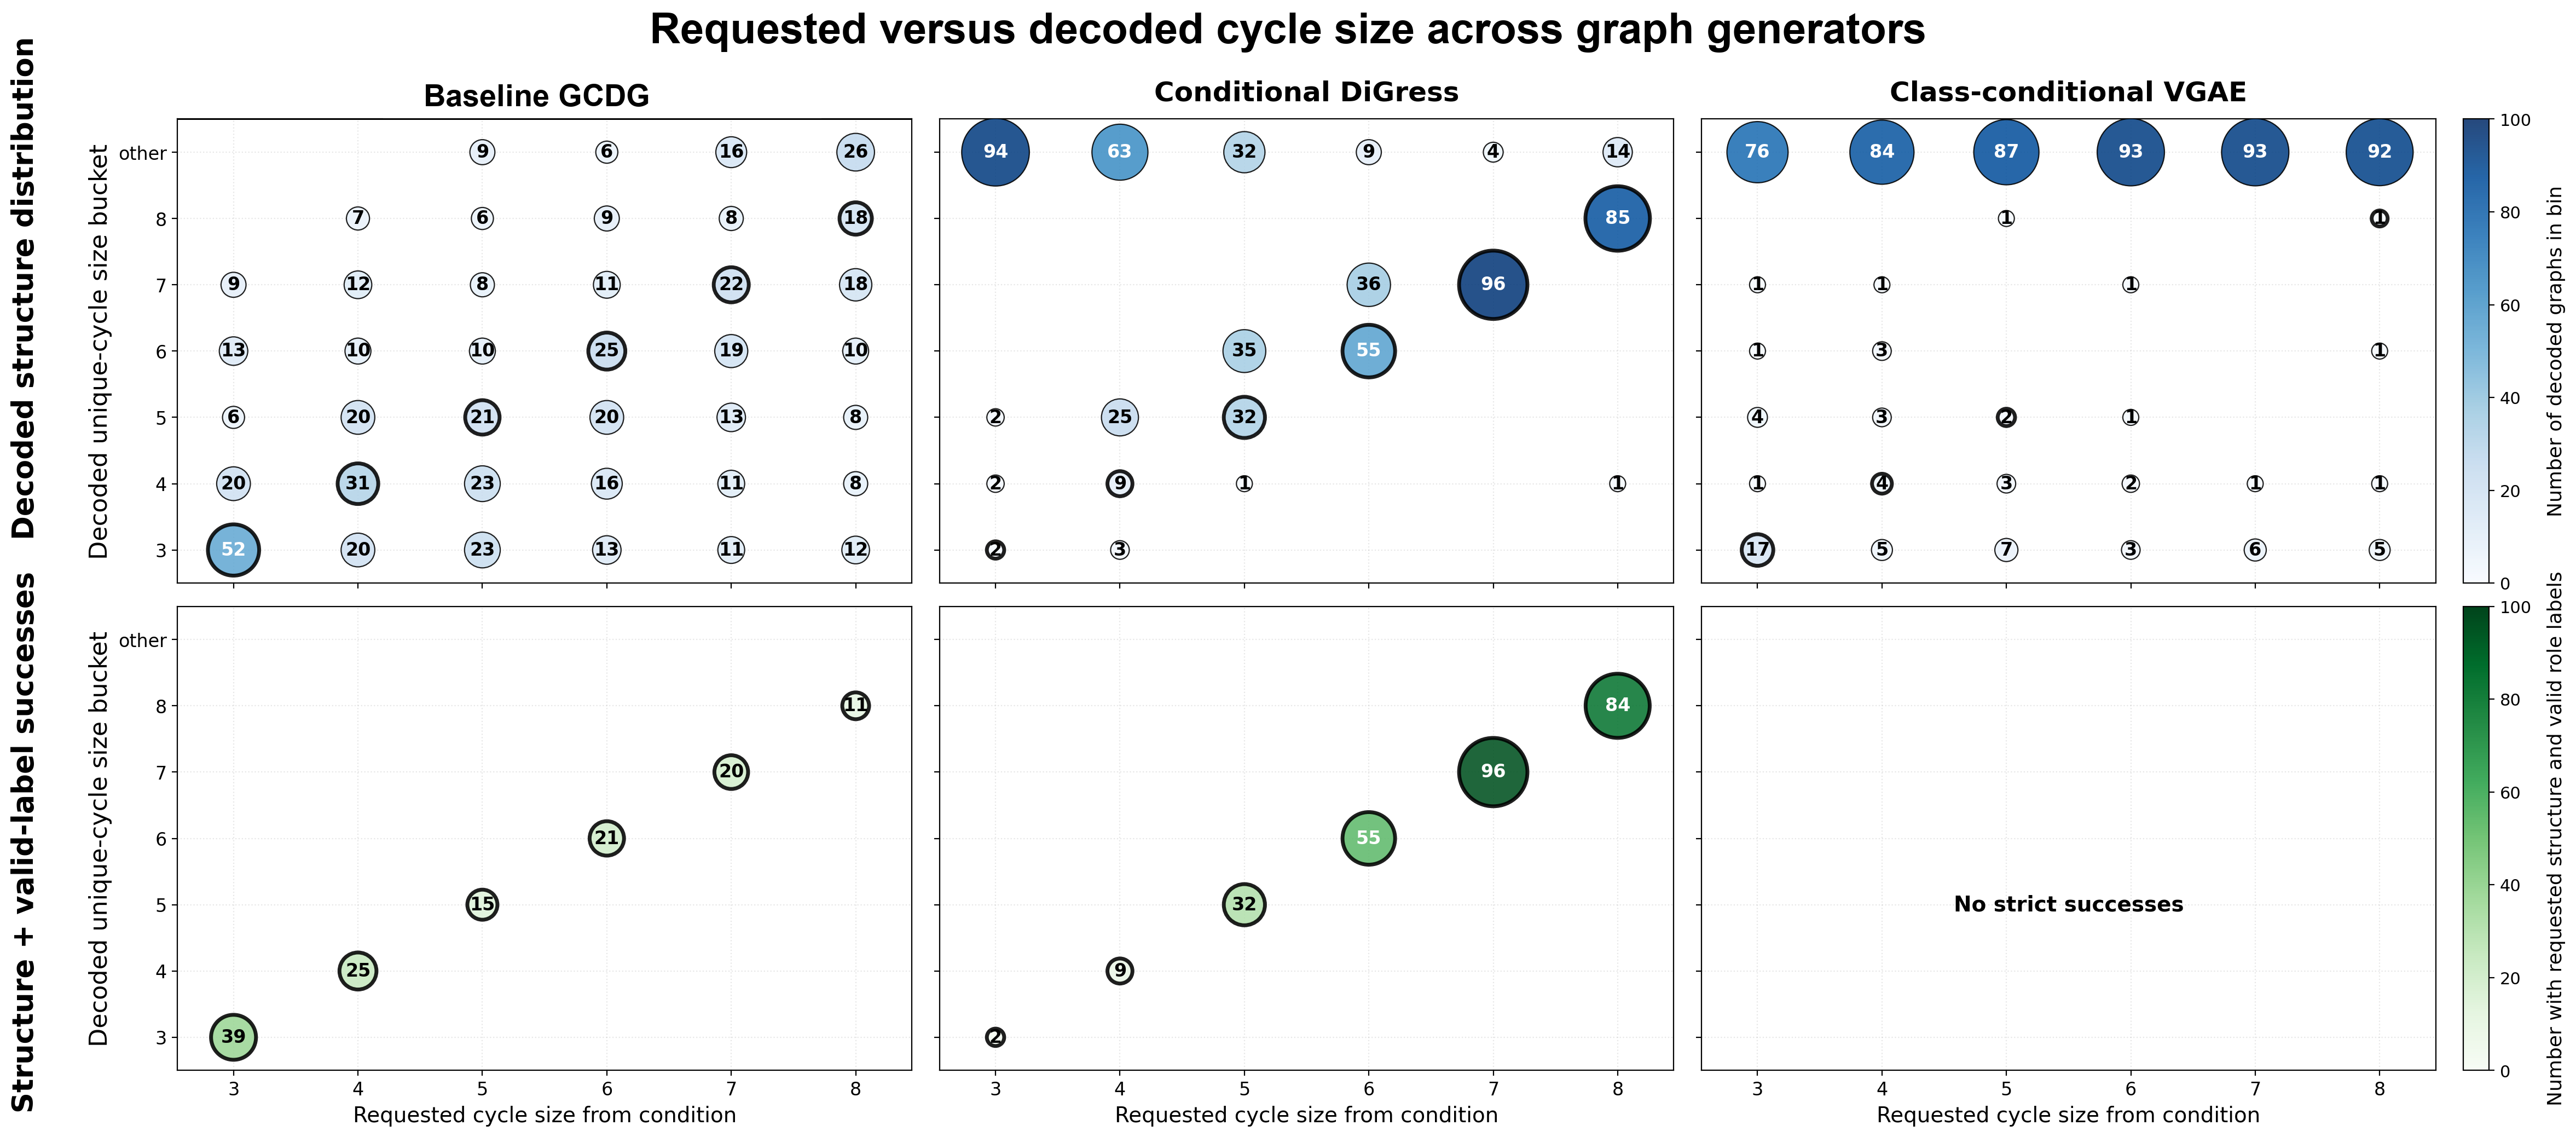
\includegraphics[
        width=1.2\textwidth,
        height=0.70\textheight,
        keepaspectratio
    ]{images/diffusion/req_vs_decoded_cycle.png}
    }
    \caption{
    Qualitative and aggregate results for the synthetic cycle--leg experiment.
    Top: examples of held-out condition graphs and generated outputs. These
    examples are illustrative; only nine generated graphs are shown for each
    displayed setting. Bottom: aggregate requested-versus-decoded cycle-size
    counts over all \(100\) generated samples per requested cycle size. In the
    bottom panel, the top row shows the decoded structure distribution and the
    bottom row counts strict successes where both the requested cycle size and
    role labels are correct. The \emph{other} bucket denotes outputs that do
    not have the required cycle--leg form, for example graphs with incoherent
    structure rather than a single cycle with one path attachment.
    }
    \label{fig:generator:req-vs-cycle-combined}
    \label{fig:generator:req-vs-gen-examples}
    \label{fig:generator:req-vs-decoded-cycle}
\end{figure}

Figure~\ref{fig:generator:req-vs-cycle-combined} first gives a qualitative view
of the experiment, showing examples of condition graphs and generated outputs.
The examples make the failure modes visually apparent, but they should not be
read as frequencies. The lower panel therefore reports the corresponding
aggregate counts out of \(100\) generated graphs per requested cycle size.

The aggregate counts show that the three models fail in different ways. The
GCDG has the broadest coverage of the cycle--leg family and
produces relatively few samples in the \emph{other} bucket. Its advantage is
clearest for the smallest requested cycles. For requested cycle sizes \(3\) and
\(4\), GCDG produces \(52\) and \(31\) exact structural matches, respectively,
compared with \(2\) and \(9\) for conditional DiGress. The same pattern appears
in the strict structure-plus-label counts: GCDG produces \(39\) and \(25\)
strict successes for cycle sizes \(3\) and \(4\), whereas conditional DiGress
produces \(2\) and \(9\).

Conditional DiGress shows the opposite behaviour. It places most cycle-three
and cycle-four requests in the \emph{other} bucket, but becomes very accurate
for larger requested cycles. For cycle sizes \(6\), \(7\), and \(8\), it
produces \(55\), \(96\), and \(84\) strict successes, respectively. GCDG still
often generates cycle--leg-like graphs for these larger conditions, but its
mass is spread across neighbouring cycle-size buckets rather than concentrated
on the requested size. The class-conditional \gls{vgae} baseline mostly
produces outputs in the \emph{other} bucket and has no strict successes,
indicating that class-level conditioning alone is not enough for this
graph-level conditional task.

This experiment isolates the role of the conditioning mechanism. A model can
generate plausible-looking graphs while still failing the conditional task. The
strict metric is therefore the rate of graphs that match both the requested
structure and the required label pattern, while the structure-distribution
panel is important for identifying whether failures remain within the intended
cycle--leg family or leave that family altogether.

\subsection{Molecular Conditional Generation}

The second set of experiments evaluates the same generator on molecular graphs.
Here the graph-level condition is computed from molecular graphs, and generation
is tested on held-out conditions not used for training. This setting asks
whether the generator can map a graph-level molecular description to a new
decoded molecular graph while maintaining chemical validity and distributional
similarity.

Generated molecules are compared with the held-out conditioning molecules that
produced them and with a reference sample from the training set. The molecular
analysis reported here focuses on two views. First, RDKit drawings provide a
qualitative inspection of generated molecular structure. Second,
distributional agreement is measured using scalar-property \gls{mmd} for
molecular weight, logP, QED, TPSA, density, atom count, bond count, and mean
bond degree. Additional validity, copying, novelty, and uniqueness diagnostics
were computed during the experimental workflow, but the main chapter reports
the RDKit visualisations and the distributional \gls{mmd} comparison.

The same held-out molecular condition set is used for the conditional
DiGress-style comparison. In both models, the condition is constructed in the
same way: a high-dimensional \gls{nsppk} graph feature vector is computed, a
truncated \gls{svd} projection fitted on the training graphs maps it to a
128-dimensional vector, and this fitted projection is then frozen and reused for
all held-out and generated graphs. Each held-out condition produces one
generated molecule. This makes the comparison a test of the generator rather
than a test of different condition vectors. The exact molecular dataset,
conditioning, training, and sampling settings are listed in
Appendix~\ref{app:qm9-molecular-settings}.

Because this is conditional generation, the evaluation also compares each
generated graph with the particular condition that produced it. For scalar graph
and molecular properties, condition-versus-generated scatter plots show whether
the generator preserves the requested property at the level of individual
conditions. For graph-level vector preservation, the generated graph is
re-encoded as \(\hat{C}\) and compared with the original condition \(C\) using
same-dimension correlations, pairwise cosine similarities, and pooled
condition-versus-re-encoding scatter plots.

\begin{figure}[t]
    \centering
    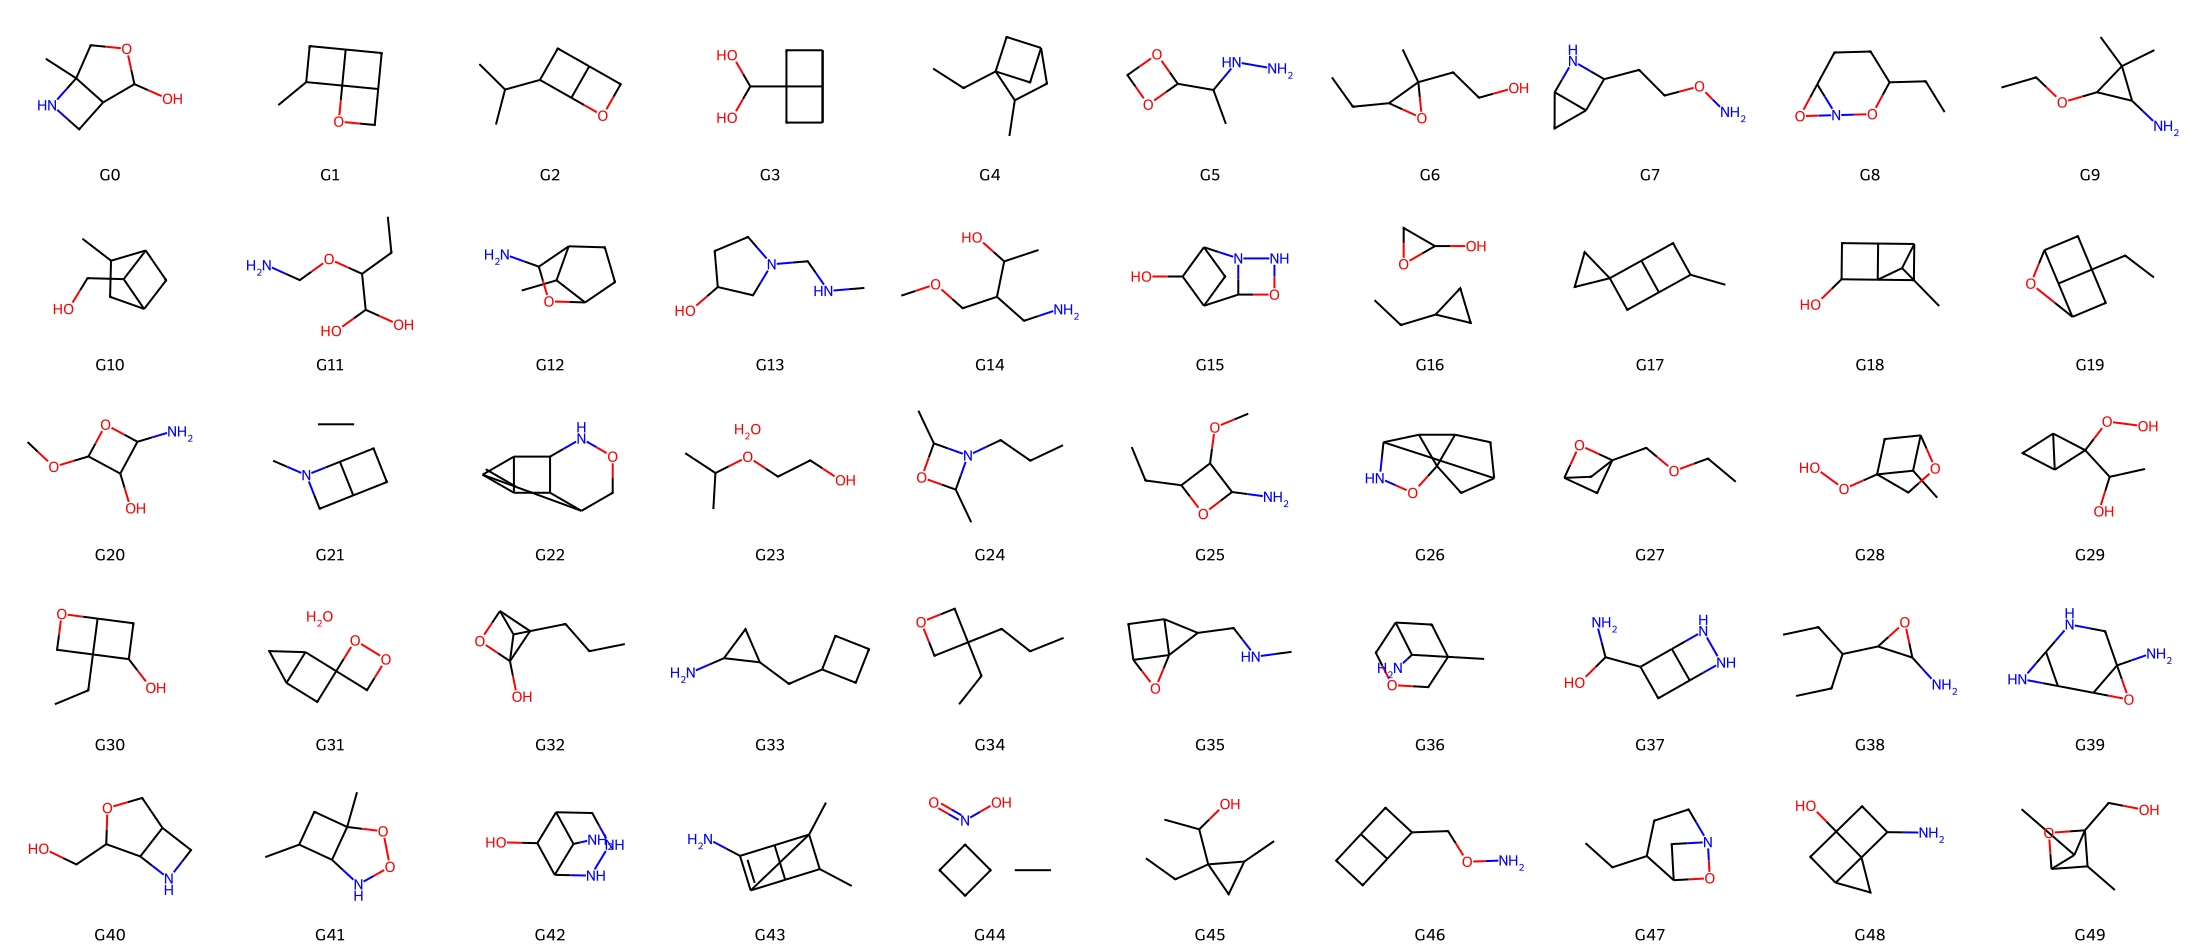
\includegraphics[
        width=\textwidth,
        keepaspectratio
    ]{images/diffusion/example_generated_my_generator.png}
    \caption{
    RDKit visualisations of QM9-like molecules generated by GCDG from held-out
    graph-level molecular conditions. These examples are qualitative samples;
    aggregate distributional comparisons are reported separately.
    }
    \label{fig:generator:qm9-gcddg-rdkit-examples}
\end{figure}



\begin{table}[t]
\centering
\footnotesize
\resizebox{\textwidth}{!}{%
\begin{tabular}{@{}lrrrrrrrr@{}}
\toprule
Model & Density & logP & Mean bond degree & Mol. weight & Bond count & Atom count & QED & TPSA \\
\midrule
GCDG & 0.006580 & 0.001988 & 0.000733 & 0.123563 & 0.008957 & 0.022764 & 0.075740 & 0.000935 \\
Conditional DiGress & 0.018580 & 0.001884 & 0.021891 & 0.010599 & 0.020499 & \(5.60\times10^{-7}\) & 0.000709 & 0.001297 \\
\bottomrule
\end{tabular}%
}
\caption{
Scalar-property \(\mathrm{MMD}^2\) between molecules generated from held-out
conditions and the held-out molecules that supplied those conditions. Smaller
values indicate closer agreement with the conditioning-molecule distribution.
Only the generated-versus-held-out-condition comparison is shown.
}
\label{tab:qm9-generated-vs-heldout-mmd}
\end{table}

Table~\ref{tab:qm9-generated-vs-heldout-mmd} shows complementary behaviour.
GCDG more closely matches structural graph statistics such as
density, mean bond degree, and bond count. Conditional DiGress more closely matches
molecular-size and chemistry-related descriptors such as atom count, molecular
weight, and QED.

\subsection{Synthetic Ablations}
\label{sec:generator:synthetic-ablations}

The synthetic cycle--leg task also provides a controlled setting for testing
which parts of the generator are needed for conditional graph construction. The
baseline setting is the Baseline GCDG configuration shown in the left column of
Figure~\ref{fig:generator:req-vs-cycle-combined} and specified in
Appendix Table~\ref{tab:synthetic-cycle-leg-proposed-hyperparameters}. Each
non-baseline ablation changes the named component and is evaluated using the
same \(100\) decoded graphs per requested cycle size. The exact cycle rate
counts graphs with the requested cycle size, while the stricter metric
additionally requires the node labels to match the required structural roles.
The Baseline GCDG row therefore corresponds to
the diagonal counts in the GCDG panels of
Figure~\ref{fig:generator:req-vs-cycle-combined}: \(169\) exact structural
matches and \(131\) strict structure-and-label matches out of \(600\) decoded
graphs.

\begin{table}[p]
\centering
\footnotesize
\begin{tabularx}{\textwidth}{@{}Xrr@{}}
\toprule
Configuration & Exact cycle rate & Strict rate \\
\midrule
Baseline GCDG & 0.282 & 0.218 \\
No degree-histogram control & 0.058 & 0.038 \\
No node-count control & 0.170 & 0.028 \\
No node-label histogram control & 0.242 & 0.110 \\
Matched-row loss enabled & 0.225 & 0.120 \\
Joint edge-state variant enabled & 0.155 & 0.017 \\
Random row permutation enabled & 0.248 & 0.168 \\
No distance supervision & 0.233 & 0.128 \\
Balanced degree loss enabled & 0.275 & 0.217 \\
No balanced edge loss & 0.280 & 0.197 \\
No node-feature dimensionality reduction & 0.175 & 0.005 \\
No clean-\(X_0\) reconstruction loss & 0.143 & 0.032 \\
No denoising-consistency loss & 0.297 & 0.235 \\
No balanced node-label loss & 0.250 & 0.162 \\
No node-label loss & 0.172 & 0.022 \\
No edge-existence loss & 0.125 & 0.008 \\
No node-existence loss & 0.217 & 0.120 \\
No degree loss & 0.163 & 0.007 \\
No edge supervision & 0.197 & 0.005 \\
No MST warm start & 0.203 & 0.095 \\
No connectivity constraint & 0.223 & 0.172 \\
No existence projection during sampling & 0.188 & 0.082 \\
No degree projection during sampling & 0.228 & 0.175 \\
No node-label projection during sampling & 0.193 & 0.050 \\
Degree and node-label channels denoised continuously & 0.243 & 0.155 \\
\bottomrule
\end{tabularx}
\caption{
Ablation results on the synthetic cycle--leg task. The Baseline GCDG row uses
the configuration specified in
Appendix Table~\ref{tab:synthetic-cycle-leg-proposed-hyperparameters}. Each
rate is computed over \(600\) decoded graphs:
\(100\) samples for each of the six requested cycle sizes. Exact cycle rate is
the fraction of decoded graphs that recover the requested cycle size, while
strict rate is the fraction that also recover the correct cycle and leg role
labels. Each non-baseline row changes the named component relative to the
Baseline GCDG configuration.
}
\label{tab:generator:synthetic-ablation-results}
\end{table}

Table~\ref{tab:generator:synthetic-ablation-results} shows that conditioning
controls and supervised structural heads have different effects. Removing the
degree-histogram control causes the largest drop in exact cycle recovery,
showing that the graph-level condition alone is not sufficient unless the
decoder is also supplied with a stable degree-composition target. Removing
node-count control, node-label histogram control, node-label supervision,
degree supervision, or the clean-\(X_0\) reconstruction loss mainly damages the
strict score, which means that the generator can still produce cycle-like
graphs but loses the alignment between structure and labels.
Removing distance supervision gives a smaller but still visible drop in both
rates, indicating that binned pairwise-distance targets help the model place
the requested cycle but are not the only structural signal used by the decoder.

The edge-supervision ablation is particularly informative. When edge
supervision is disabled, the learned pairwise edge-probability head is no
longer available and decoding falls back to degree-based edge scores. The
resulting graphs remain structurally feasible in a coarse sense: in the
recorded run all decoded graphs were connected, and the mean number of edges
matched the mean number of nodes in each requested category. However, the strict
rate falls from \(0.218\) to \(0.005\). This indicates that degree and
connectivity constraints can still force the decoder towards unicyclic graphs,
but they do not replace learned pairwise information about where the cycle and
leg edges should be placed or how labels should align with that structure.

Some components are less critical in this synthetic setting. Removing the
denoising-consistency loss slightly improves both reported rates, suggesting
that this auxiliary term is not necessary for the cycle--leg benchmark. Balanced
degree and edge losses also have small effects relative to the main structural
supervision terms. These ablations support the design used in the main
experiment: GCDG works best when the graph-level condition is coupled to
explicit node-count, degree, label, and pairwise-edge predictions before the
constraint-aware decoder constructs the final discrete graph.

\section{Limitations}
\label{sec:generator:limitations}

The staged design also introduces limitations. First, the quality of generation
depends on the node representation. If the node feature matrix does not contain enough
information to distinguish structurally important roles, the denoiser may match
global statistics while placing labels incorrectly. Second, the constrained
decoder can correct some structural inconsistencies, but it cannot recover
information that the denoiser failed to represent. Third, the integer
optimisation step improves feasibility but may become expensive for larger
graphs or dense candidate edge sets.

A further limitation is that chemistry-aware rules, when enabled, are not the
same as learning chemistry from data alone. Valency projection can improve
RDKit validity by removing or downgrading invalid bonds, but this should be
reported as a post-processing constraint rather than as unconstrained neural
generation. Similarly, dynamic molecular features provide the denoiser with
state-dependent chemical summaries; they are appropriate for molecular
ablations but are not part of the generic graph generator.

Finally, the model is conditional on a graph-level vector \(C\). Strong
conditioning performance therefore depends on the informativeness and stability
of this vector. In the experiments, condition consistency is assessed through
proxy comparisons with the held-out graphs that supplied the condition:
structural statistics, molecular properties, and correlations between the
condition vector \(C\) and the re-encoded generated graph \(\hat{C}\). These
comparisons test whether the generated graph preserves information encoded in
the condition, rather than whether it reconstructs the conditioning graph
exactly.

\section{Summary}
\label{sec:generator:summary}

This chapter introduced the Graph-Conditioned Diffusion Generator, a
conditional graph generator that maps a fixed graph-level descriptor to a
discrete labelled graph. The method separates the continuous reverse diffusion
process over padded node features from the later decisions that determine node
existence, node labels, degree classes, edge probabilities, and edge labels.
The final graph is obtained by a constraint-aware decoder, so graph feasibility
is handled explicitly rather than being left entirely to the neural denoising
network.

The synthetic cycle--leg experiment shows why this staging is useful. The model
does not merely generate plausible graphs; it can be evaluated against explicit
conditional requirements such as requested cycle size and role-label placement.
The comparison with conditional DiGress and a class-conditional \gls{vgae}
baseline shows that different generators fail in different ways: GCDG performs
best on the smallest requested cycles and produces fewer samples outside the
intended cycle--leg family, whereas DiGress is much stronger on the larger
requested cycles.

The QM9 experiment extends the same conditioning mechanism to molecular graphs.
In this chapter, the molecular results are reported through RDKit
visualisations and scalar-property \gls{mmd} comparisons between generated
molecules and the held-out molecules that supplied their conditions. 
The results should be interpreted as a conditional distributional comparison
rather than as a complete molecular benchmark. They show that GCDG
matches some structural graph statistics closely, whereas the conditional
DiGress-style model better matches molecular-size and chemistry-related
descriptors such as atom count, molecular weight, and QED.

Overall, the chapter establishes GCDG as a graph-conditioned diffusion
generator in which continuous node-feature generation and discrete graph
construction are deliberately separated. The experiments show that this design
can preserve explicit conditional structure in the synthetic setting, while the
molecular setting exposes the additional difficulty of matching chemical and
property-level constraints. These results motivate the next chapter, which
turns from generator design to the broader problem of evaluating generated data
with diagnostic, statistically grounded probes.

\chapter{RankGen: Diagnostic Evaluation of Generative Models}
\label{ch:rankgen}

\section{Introduction and Motivation}
\label{sec:rankgen:intro}

Chapter~\ref{ch:theory} established the theoretical foundations for this
thesis, introducing graphs as structured data objects, reviewing
representation learning methods, and discussing the principles underlying
modern generative models. While these developments have enabled increasingly
powerful models for generating structured data, they also raise a fundamental
question: \emph{how should the quality of generative models be evaluated in a
way that is reliable, interpretable, and relevant to downstream tasks?}

Generative models are now widely used across domains such as image synthesis,
molecular design, graph generation, and natural language processing.
In many cases, these models produce samples that appear realistic or
domain-valid. However, visual or qualitative inspection alone is insufficient
for rigorous comparison between models, and reliable automated evaluation
remains an open challenge.

Many widely used evaluation metrics are brittle, easy to manipulate, and often
poorly aligned with the practical value of generated data. Standard metrics may
assign high scores to models that memorise training data, fail to generalise,
or provide little benefit in downstream predictive tasks. As a result, model
selection based solely on such scores can lead to unreliable conclusions and
potentially unsafe deployment decisions.

A large body of work has highlighted these limitations. Single-number
heuristics such as the Inception Score (IS)~\citep{salimans2016improved} and
Fr\'echet Inception Distance (FID)~\citep{heusel2017gans}, together with
kernel-based distances such as MMD and KID
\citep{gretton2012kernel,binkowski2018demystifying}, provide convenient scalar
summaries of generative performance. However, these metrics rely on strong
assumptions about feature representations and distributional structure.
In practice, they are sensitive to implementation choices, preprocessing
pipelines, and the particular feature extractor used to embed samples
\citep{barratt2018note,chong2020effectively,parmar2022aliased,
jayasumana2024rethinking,betzalel2022study}. Moreover, reducing generator
performance to a single scalar collapses distinct aspects of generative
behaviour---such as fidelity, diversity, and task relevance---and can obscure
important failure modes including mode collapse or data copying.

To address these limitations, several works propose multi-dimensional
evaluation summaries. Metrics such as precision--recall for distributions
\citep{sajjadi2018assessing,kynkaanniemi2019improved} and density--coverage
\citep{naeem2020reliable} attempt to separate aspects of fidelity and support,
providing more nuanced diagnostic information. Nevertheless, these approaches
remain strongly dependent on representation choices and typically lack
statistical guarantees about the reliability of the reported scores.Classifier-based evaluation protocols move closer to practical utility.
Methods such as GAN-train/test~\citep{shmelkov2018good} and
train-on-synthetic, test-on-real (TSTR)
\citep{hyland2017real,esteban2017real,yoon2019timegan} evaluate whether
generated data supports predictive tasks. However, these protocols are
typically reported as point estimates and provide little insight into the
statistical reliability of the observed results.

A particularly important risk is \textbf{memorisation}. Generative models may
replicate training data, artificially inflating similarity metrics while
providing little additional information and potentially exposing sensitive
training examples~\citep{bhattacharjee2023data}. Recent work has demonstrated
that diffusion and GAN models can leak training samples through extraction
attacks ~\citep{carlini2023extracting,hayes2019logan,chen2020ganleaks}, yet
many commonly used evaluation scores fail to detect such behaviour.

\begin{figure}[t]
  \centering
  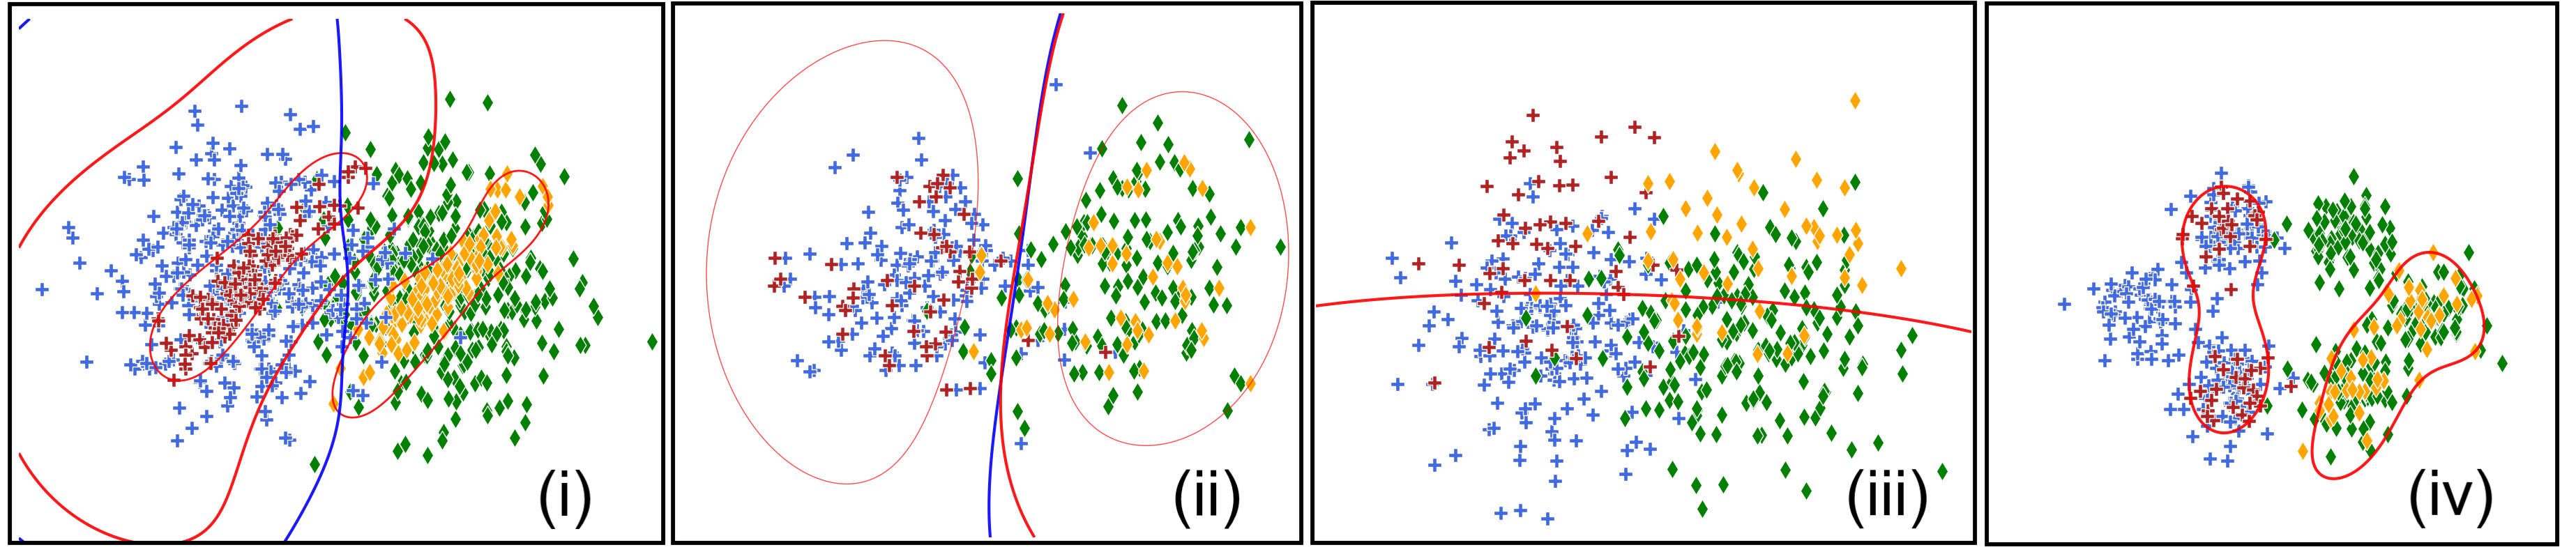
\includegraphics[width=1\linewidth]{images/rankgen/metrics.png}
  \caption{Four common generative failure modes and how RankGen detects them.
Each panel shows real data (blue and green) and generated data (red and orange)
for a binary classification task. Marker shapes denote classes.}
  \label{fig:generated-results}
\end{figure}
These challenges highlight a broader issue: generative model evaluation is
inherently multi-dimensional. A generator may preserve task-relevant signal,
yet still be easy to distinguish from real data. It may align globally with the
data distribution but fail to provide useful new information.

Figure
\ref{fig:generated-results} illustrates several such failure modes. Each panel shows real data (blue/green) and generated data (red/orange) for a binary classification task, with marker shapes indicating class labels. (i) \emph{Quality (poor task fidelity):} Generated samples lie in high-density regions of the real distribution but fail to produce a decision boundary that generalises, leading to poor classifier performance when trained on synthetic data. (ii) \emph{Utility (no added value):} Generated samples closely replicate the real data; augmenting the training set with them neither improves performance nor alters the decision boundary. (iii) \emph{Indistinguishability (easy to distinguish):} A subtle artefact (e.g., a shift in a single feature) allows a discriminator to separate real from generated samples, despite their apparent global similarity. (iv) \emph{Similarity (local mismatch):} Local neighbourhoods are dominated by either real or generated samples, indicating poor mixing due to structural differences or mode collapse; this is captured by neighbourhood entropy even when global distributions overlap.
\section{Limitations of Existing Evaluation Approaches}
\label{sec:rankgen:limitations}

Chapter~\ref{ch:theory} reviewed the principal families of metrics used to
evaluate generative models, including scalar heuristics, distributional
distances, and classifier-based evaluation protocols. While these approaches
provide useful insight, they also exhibit important limitations that make
reliable comparison between generative models difficult. In this section we
briefly revisit these approaches and highlight the specific shortcomings that
motivate the RankGen framework.

Many generative models are evaluated using single-number metrics such as the
Inception Score (IS)~\citep{salimans2016improved}, the Fr\'echet Inception
Distance (FID)~\citep{heusel2017gans}, or kernel-based distances such as
Maximum Mean Discrepancy (MMD) and Kernel Inception Distance (KID)
\citep{gretton2012kernel,binkowski2018demystifying}. These metrics are widely
used because they provide convenient scalar summaries that allow models to be
ranked easily.

However, such metrics rely on strong assumptions about the representation space
used to embed samples. Their values can vary substantially depending on the
choice of feature extractor, preprocessing pipeline, or evaluation protocol
\citep{barratt2018note,chong2020effectively,parmar2022aliased,betzalel2022study}.
Moreover, compressing generative behaviour into a single scalar inevitably
conflates multiple aspects of performance, including fidelity, diversity, and
task relevance. As a consequence, these metrics often fail to reveal important
failure modes such as mode collapse or data copying.

To address these shortcomings, several works propose multi-dimensional
evaluation summaries that separate different aspects of generative behaviour.
Examples include precision--recall for distributions
\citep{sajjadi2018assessing,kynkaanniemi2019improved} and density--coverage
metrics~\citep{naeem2020reliable}. These approaches provide richer diagnostic
information by distinguishing between fidelity and support coverage.

Despite these improvements, such metrics remain highly dependent on the
representation space used to compare samples. Small changes in embedding
choices or feature extraction pipelines can significantly alter the reported
scores. Furthermore, most of these methods remain descriptive rather than
inferential: they quantify differences between datasets but rarely provide
statistical guarantees regarding the reliability of the observed comparisons.

A different line of work evaluates generative models through predictive tasks.
Protocols such as GAN-train/test~\citep{shmelkov2018good} and
train-on-synthetic, test-on-real (TSTR)
\citep{hyland2017real,esteban2017real,yoon2019timegan} measure whether
generated data supports supervised learning tasks. This perspective is
particularly appealing because it directly relates generative performance to
downstream predictive utility.

However, these evaluations are typically reported as point estimates without
uncertainty quantification. Differences between models may therefore reflect
sampling noise or training variability rather than genuine differences in
generative quality. In addition, a single predictive score often conflates
multiple potential failure modes, such as insufficient diversity, poor signal
fidelity, or overfitting to the training data.

An especially problematic failure mode is memorisation. Generative models may
reproduce training samples or near-duplicates, artificially inflating
similarity metrics while contributing little additional information.
Beyond limiting the usefulness of generated data, memorisation also raises
important privacy concerns when sensitive training samples can be reconstructed
or extracted from a trained generator
\citep{bhattacharjee2023data,carlini2023extracting,hayes2019logan,chen2020ganleaks}.
Many widely used evaluation protocols fail to detect such behaviour.

Taken together, these observations reveal that existing evaluation approaches
provide only partial insight into the behaviour of generative models.
Scalar metrics are simple but brittle, distributional diagnostics are more
informative but representation-dependent, and classifier-based evaluations
align with practical utility but lack statistical guarantees.

These limitations motivate the RankGen framework developed in this chapter:
an evaluation protocol that uses predictive probes to separate different
failure modes, attaches reliability checks to the resulting estimates, and
uses robust summaries when comparing generators.

\section{RankGen Contribution and Chapter Structure}
To address these challenges, this chapter introduces \textbf{RankGen}, a
classifier-based evaluation framework that treats generator assessment as a
set of predictive probes. The framework defines four metrics: \emph{Quality}
(signal fidelity), \emph{Utility} (added predictive value beyond real data),
\emph{Indistinguishability} (two-sample alignment), and \emph{Similarity}
(local structural mixing between real and generated samples). Each metric is
paired with a PAC-style reliability check for the corresponding empirical
estimate. Candidate generators are then evaluated through a four-stage
protocol: data preparation, probe training, reliability filtering, and robust
ranking. A composite score, \emph{Exchangeability}, aggregates the accepted
signals to summarise predictive usefulness and distributional alignment.

The contribution of the chapter is therefore not another single score, but a
diagnostic protocol for asking which aspect of generation fails, whether the
evidence is reliable under the chosen probes, and how surviving models should
be ranked across repeated evaluations. The empirical sections test this
protocol on controlled perturbations, molecular graph generators, image
benchmarks, and open-domain text generation.

\paragraph{Chapter structure.}
The remainder of this chapter is organised as follows. The preceding section
identified limitations of existing evaluation approaches and motivated the need
for a diagnostic framework with explicit reliability checks.
Section~\ref{sec:rankgen:framework} reformulates generative model evaluation
as a learning problem.
Section~\ref{sec:method} presents the RankGen methodology, including the data
preparation pipeline, classifier-based probes, PAC-style guarantees,
quantile-based aggregation, and the ranking procedure.
Section~\ref{sec:empirical} reports empirical results on controlled synthetic
perturbations, molecular graph datasets, image benchmarks, and open-domain
text generation.
Finally, Section~\ref{sec:conclusion-rankgen} concludes the chapter and
summarizes its main findings.



\section{Evaluation as a Learning Problem}
\label{sec:rankgen:framework}

The limitations of existing evaluation metrics suggest that assessing
generative models cannot be reduced to computing a single similarity score
between real and generated datasets. Instead, evaluation must capture how
generated samples interact with real data in tasks that reflect the intended
use of the generator.

A useful perspective is to view generative model evaluation through the lens
of statistical learning theory. In this view, generated samples are treated as
data produced by an alternative distribution, and evaluation is formulated as
a collection of predictive tasks designed to probe different aspects of the
relationship between the generated and real distributions.

Let $P_r$ denote the real data distribution and $P_g$ the distribution induced
by a generative model.
by a generative model. Given samples from these distributions, we construct
learning problems whose solutions reveal properties of the generator.
Different predictive tasks expose different types of failure modes.

For example, if a classifier trained on generated data generalises poorly to
real data, this suggests that the generator fails to capture task-relevant
structure. Conversely, if a classifier can easily distinguish real from
generated samples, this indicates a distributional mismatch between $D_r$ and
$D_g$. If generated samples provide no improvement when added to real training
data, this suggests that the generator contributes little new information.

This perspective leads naturally to the idea of \emph{evaluation probes}.
Each probe is a supervised learning problem designed to measure a specific
property of the generator. By observing how predictive models behave under
different training configurations involving real and generated data, it is
possible to infer properties of the underlying generative distribution.

Importantly, framing evaluation in this way enables the use of tools from
learning theory to reason about reliability. Instead of reporting raw
empirical scores, evaluation results can be accompanied by statistical
generalisation guarantees that bound the discrepancy between observed
performance and true performance on unseen data.

Within this framework, generative model evaluation becomes a structured
procedure consisting of multiple predictive probes, each targeting a
different potential failure mode.

\section{The Method: RankGen}
\label{sec:method}

\textbf{RankGen} evaluates generative models through a statistically grounded,
classifier-based framework that jointly measures predictive usefulness and
distributional alignment. Rather than relying on a single similarity score,
RankGen decomposes evaluation into complementary probes and combines them
with PAC-style guarantees and robust statistical summaries.

Evaluating generative models requires balancing \emph{reliability} and
\emph{resolution}. RankGen explicitly separates these roles:
(i) \emph{PAC-style bounds} act as \emph{reliability gates}, ensuring that
reported scores hold with high probability, and
(ii) \emph{quantile-based summaries} (median and IQR) provide resolution,
capturing central tendency and variability across stochastic trials.
Together, these prevent unreliable models from being ranked while enabling
fine-grained comparison among valid ones.

\paragraph{Pipeline overview.}
RankGen follows a four-stage evaluation pipeline:

\textbf{(1) Data preparation and sampling.}
We generate multiple stochastic replicates using stratified bootstrap splits of
the labelled dataset. For each replicate, we construct
$D_{\text{train1}}^{(i)}$, $D_{\text{train2}}^{(i)}$, and a fixed
$D_{\text{test}}$. Generators are trained on
$D_{\text{train1}}^{(i)}$ and produce class-conditional synthetic samples,
yielding $D_{\text{generated}}^{(i)}$.

\textbf{(2) Metric evaluation.}
We evaluate generators using four classifier-based probes:
\emph{Quality} (signal fidelity),
\emph{Utility} (added predictive value),
\emph{Indistinguishability} (real vs.\ generated separability), and
\emph{Similarity} (local structural mixing).
Each metric captures a distinct failure mode and is computed under a unified
evaluation protocol.

\textbf{(3) Statistical aggregation.}
For each metric, we compute PAC-style generalisation bounds to ensure
statistical reliability, and aggregate results across replicates using robust
quantile summaries (median and IQR). This yields stable, uncertainty-aware
estimates of generator performance.

\textbf{(4) Ranking and diagnosis.}
We first filter generators based on bound violations (pass/fail per metric),
retaining only statistically reliable candidates. Within each group, models
are ranked using quantile summaries and pairwise dominance. Finally, the joint
metric profile is used for \emph{diagnosis}: for example, high similarity but
low utility indicates copying, while high quality but low indistinguishability
suggests distributional mismatch.

\medskip
This multi-dimensional view enables RankGen to move beyond scalar evaluation,
providing both reliable ranking and interpretable insights into how and why
generators succeed or fail.
\begin{figure}[H]
    % \centering
    \hspace{-1.25cm}
    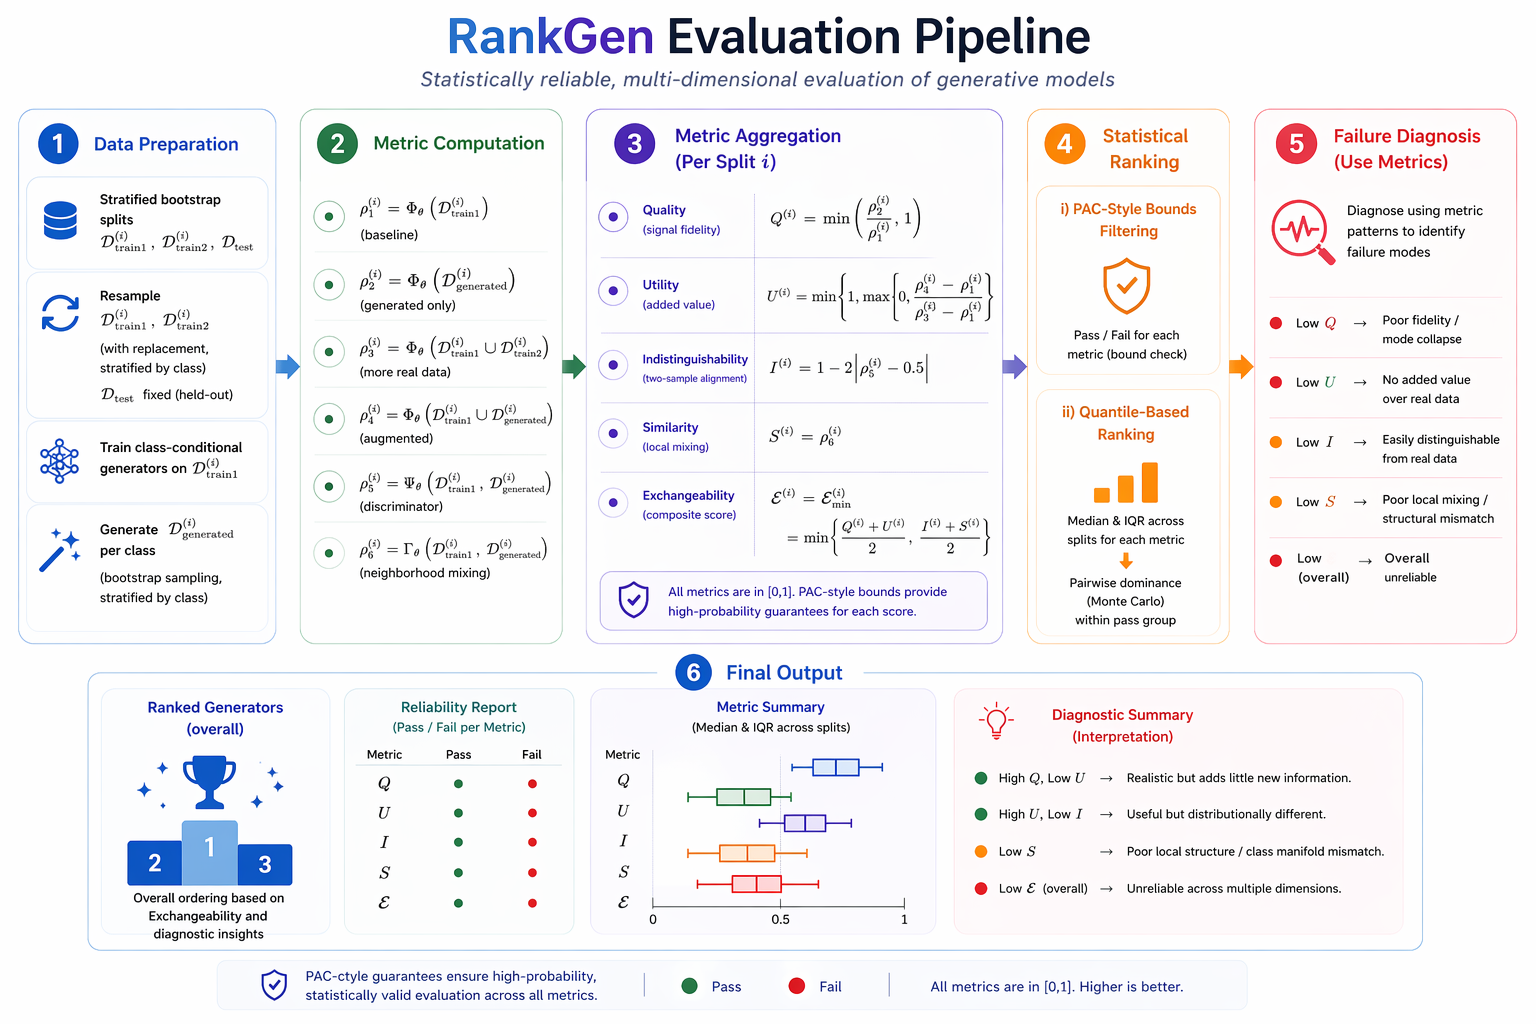
\includegraphics[width=1.25\linewidth]{images/rankgen/pipeline_final.png}
    \caption{
    \textbf{RankGen evaluation pipeline.}
    The framework consists of four stages:
    (1) \emph{Data preparation} via stratified bootstrap splits and class-conditional generation;
    (2) \emph{Metric evaluation} using classifier-based probes (Quality, Utility, Indistinguishability, Similarity);
    (3) \emph{Statistical aggregation} combining PAC-style reliability bounds with quantile summaries;
    and (4) \emph{Ranking and diagnosis}, where generators are filtered by pass/fail checks and ranked using robust statistics, with metric profiles used to diagnose failure modes.
    }
    \label{fig:rankgen_pipeline}
\end{figure}
%-------------------------------------------------------------------------------------------------------------
\subsection{Data Preparation and Sampling}

Consider a classification dataset \(D = \{(x_i, y_i)\}_{i=1}^N\),
where each feature vector \(x_i \in \mathbb{R}^d\) lies in a \(d\)-dimensional space,
and each label \(y_i \in \{1,\ldots,C\}\) denotes one of \(C\) classes.
We first partition \(D\) into a training set \(D_{\text{train}}\) and a held-out
test set \(D_{\text{test}}\).
The training set is then further divided, using stratified sampling, into two
equally sized subsets, \(D_{\text{train1}}\) and \(D_{\text{train2}}\).


\paragraph{Training the generators.}
We adopt a class-wise strategy for generating synthetic data.
Unless the underlying model is inherently class-conditional, we train a separate
generator for each class.
Specifically, for every class \(c \in \{1,\ldots,C\}\), we fit a generative model \(f_c\) using only
the corresponding subset \(D_{\text{train1}}^{c}\) of the training data.
For models that are unconditional, we use the same generator architecture,
but train it independently on the samples of each class.
%Each generator is trained once per generator configuration, and is not retrained across replicates.


\paragraph{Constructing the synthetic pool.}
After training, we draw synthetic samples once for each class to construct a
base synthetic dataset. Let \(p_{f_c}\) denote the distribution induced by the generator \(f_c\). For each class \(c\), we sample
$
\{x_{c,\ell}\}_{\ell=1}^{N_c} \sim p_{f_c},
$ where \(N_c = |D_{\text{train1}}^{c}|\) is the desired number of generated examples for class \(c\).
The resulting synthetic dataset is then the union of all class specific samples
\[
D_{\text{generated}}
= \bigcup_{c}
\{(x_{c,\ell},\, c) : \ell = 1,\ldots,N_c\}.
\]



\paragraph{Uncertainty estimate.}
To estimate uncertainty for each replicate \(i\), we draw bootstrap samples
$
D_{\text{train1}}^{(i)} \subseteq D_{\text{train1}},\quad
D_{\text{train2}}^{(i)} \subseteq D_{\text{train2}},\quad
D_{\text{generated}}^{(i)} \subseteq D_{\text{generated}},\quad
$
using class-stratified bootstrapping.
Each replicate is used to compute all four metrics and their quantile summaries.


%-------------------------------------------------------------------------------------------------------------
\subsection{Classifier Performance Scores (\texorpdfstring{$\rho_i$}{rho\_i})}
We propose 4 key metrics: Quality, Utility, Indistinguishability, and Similarity defined via classifier-derived scores $\rho^{(i)}_j$ (Table~\ref{tab:classifier-metrics}), with every score corresponding to a distinct training-and-testing configuration on split $i$. All models are evaluated on the same shared test set $D_{\text{test}}$. Here, $\Phi_\theta$ denotes a task classifier, $\Psi_\theta$ a binary real-vs-generated discriminator, and $\Gamma_\theta$ a structure-aware similarity model (e.g., a data-specific kernel).

\begin{table}[H]
\centering
\caption{Classifier-based evaluation metrics used in \textsc{RankGen}.}
\label{tab:classifier-metrics}
\begin{small}
\begin{tabular}{@{}l p{0.65\linewidth}@{}}  % <-- wrap description
\toprule
\textbf{Metric} & \textbf{Description} \\
\midrule
$\rho_1^{(i)} = \Phi_{\theta}(D_{\text{train1}}^{(i)})$ & Accuracy of classifier trained on real data only (baseline). \\
$\rho_2^{(i)} = \Phi_{\theta}(D_{\text{generated}}^{(i)})$ & Accuracy when trained on generated data only (signal fidelity). \\
$\rho_3^{(i)} = \Phi_{\theta}(D_{\text{train1}}^{(i)} \cup D_{\text{train2}}^{(i)})$ & Accuracy with extra real data (upper bound). \\
$\rho_4^{(i)} = \Phi_{\theta}(D_{\text{train1}}^{(i)} \cup D_{\text{generated}}^{(i)})$ & Accuracy with real+generated data (usefulness). \\
$\rho_5^{(i)} = \Psi_{\theta}(D_{\text{train1}}^{(i)}, D_{\text{generated}}^{(i)})$ & Discriminator accuracy distinguishing real vs.\ generated. \\
$\rho_6^{(i)} = \Gamma_{\theta}(D_{\text{train1}}^{(i)}, D_{\text{generated}}^{(i)})$ & Entropy-based similarity of local feature neighbourhoods. \\
\bottomrule
\end{tabular}
\end{small}
\end{table}



%---------------------------------------------------------------------------------------------------------
\subsection{Quality Metric}
\label{sec:quality}

\paragraph{Definition (normalized TSTR).}
The \textbf{quality} score quantifies how much predictive signal synthetic data
carries relative to real data. On split $i$, let $\rho^{(i)}_1$ be the task
score (e.g., accuracy, AUC, or macro-F1) of a classifier $\Phi_\theta$ trained
on $D^{(i)}_{\text{train1}}$ and evaluated on $D_{\text{test}}$, and let
$\rho^{(i)}_2$ be the score of the same classifier class trained on
$D^{(i)}_{\text{generated}}$ and evaluated on $D_{\text{test}}$. We define the
normalized Train-on-Generated-Test-on-Real (TSTR) ratio
\[
Q^{(i)} := \min\!\left(\frac{\rho^{(i)}_2}{\rho^{(i)}_1},\,1\right)\in[0,1].
\]

\paragraph{generalisation bound.}
Using the PAC-learning preliminaries introduced in Chapter~\ref{ch:theory},
together with a standard domain-adaptation argument, one obtains a conservative
lower bound on the population quality score in terms of three quantities:
(i) generalisation error for the task classifier, (ii) discrepancy between the
real and generated distributions, and (iii) the joint optimal risk between the
two domains. The resulting guarantee shows that quality degrades as classifier
uncertainty or distributional mismatch increases. A full derivation and exact
bound statement are given in Appendix~\ref{app:theory-quality}.

\paragraph{Interpretation and practice.}
High values close to $1$ indicate that synthetic data preserves task-relevant
structure, whereas low values reveal fidelity gaps such as label noise, mode
collapse, or covariate shift. Any bounded task score in $[0,1]$ may be used,
but the \emph{same} score must define both $\rho^{(i)}_1$ and $\rho^{(i)}_2$ to
ensure comparability; for imbalanced labels, macro-averaged variants are often
preferable. When the real-data baseline $\rho^{(i)}_1$ is close to chance, the
ratio becomes unstable and the bound loosens; in practice, we either enforce a
minimal baseline before reporting the ratio or report the ratio alongside the
absolute scores. Across resampling trials, we aggregate $Q^{(i)}$ using robust
quantiles (median and IQR; see Sec.~\ref{sec:quantile-based-estimation}) and
use the PAC bound as a pass/fail gate prior to fine-grained ranking. If
training on synthetic data outperforms training on real
($\rho^{(i)}_2>\rho^{(i)}_1$), we cap the score at $1$ for consistency with the
other $[0,1]$ metrics used in the composite, while retaining the uncapped ratio
for diagnostic analysis if needed.


%---------------------------------------------------------------------------------------------------------
\subsection{Utility Metric}
\label{sec:utility}

\paragraph{Definition.}
The \emph{utility} score quantifies the incremental benefit of augmenting real
training data with synthetic samples. Let
\[
\Delta_{\mathrm{real}}^{(i)} := \rho_3^{(i)}-\rho_1^{(i)}
\]
denote the gain from adding more \emph{real} data, and let
\[
\Delta_{\mathrm{generated}}^{(i)} := \rho_4^{(i)}-\rho_1^{(i)}
\]
denote the gain from adding \emph{generated} data under the same augmentation
budget. We define
\[
U^{(i)} \;=\;
\min\!\Bigl\{1,\;\max\!\bigl\{0,\;
\Delta_{\mathrm{generated}}^{(i)} / \Delta_{\mathrm{real}}^{(i)}
\bigr\}\Bigr\},
\]
so that values near $1$ indicate that synthetic data is nearly as useful as
additional real data. For diagnostic purposes, we also retain the uncapped ratio
\[
\tilde U^{(i)}=
\Delta_{\mathrm{generated}}^{(i)} / \Delta_{\mathrm{real}}^{(i)}.
\]

\paragraph{Generalisation bound.}
Using the PAC-learning preliminaries from Chapter~\ref{ch:theory}, together
with a standard domain-adaptation argument, one obtains a conservative lower
bound on the population utility score in terms of three quantities: (i)
generalisation error of the task classifiers, (ii) discrepancy between the real
and generated distributions, and (iii) the joint optimal risk across the two
domains. Intuitively, the guarantee becomes weaker when generated samples are
easy to distinguish from real ones or when the gain from extra real data is very
small. A full derivation and exact bound statement are given in
Appendix~\ref{app:theory-utility}.

\paragraph{Interpretation and practice.}
Utility captures whether synthetic data contributes \emph{additional} predictive
value beyond the original real training set. When a generator merely memorises
existing samples, synthetic augmentation adds little or no new information, so
$\Delta_{\mathrm{generated}}^{(i)}$ remains small and $U^{(i)}$ collapses
toward $0$, even if other similarity-style scores appear strong. Conversely,
when the synthetic distribution is both well aligned with the real one and rich
in task-relevant variation, the gain from augmentation approaches that obtained
from additional real data, pushing $U^{(i)}$ toward $1$.

In reporting, we keep augmentation budgets matched between real and synthetic
additions, use the \emph{same} bounded task score for all $\rho_j^{(i)}$
involved, and aggregate $U^{(i)}$ across resamples using robust quantiles
(median and IQR; see Sec.~\ref{sec:quantile-based-estimation}). As with the
other metrics, we use the PAC bound as a pass/fail gate prior to fine-grained
ranking. Two practical cautions are important. First, if
$\Delta_{\mathrm{real}}^{(i)}$ is very small, the ratio becomes unstable; in
that case, we report the absolute gains alongside the ratio or revert to the
difference form discussed in Appendix~\ref{app:theory-utility}. Second, if
synthetic augmentation helps more than additional real data
($\tilde U^{(i)}>1$), we cap the reported score at $1$ for comparability in the
composite metric while retaining $\tilde U^{(i)}$ for diagnosis.
%---------------------------------------------------------------------------------------------------------
%---------------------------------------------------------------------------------------------------------
\subsection{Indistinguishability Metric}
\label{sec:indistinguishability}

\paragraph{Definition.}
Indistinguishability measures how difficult it is for a discriminator
$\Psi_\theta$ to distinguish real samples from generated ones on a held-out,
balanced evaluation set. Let $\rho^{(i)}_5$ denote the test accuracy of the
real-vs-generated discriminator on split $i$, where chance performance is
$0.5$. We define the symmetric score
\[
I^{(i)} \;=\; 1 - 2\bigl|\rho^{(i)}_5 - 0.5\bigr| \;\in\; [0,1],
\]
so that $I^{(i)}=1$ when the discriminator operates at chance, indicating that
real and generated samples are hard to separate, and $I^{(i)}=0$ when the two
domains are perfectly distinguishable. For diagnostic purposes, one may also
report the conventional quantity $1-\rho^{(i)}_5$, but we use the symmetric
mapping above to keep all base metrics on a common $[0,1]$ scale. The same
definition can also be applied with AUC in place of accuracy.

\paragraph{Generalisation bound.}
Using the PAC-learning preliminaries from Chapter~\ref{ch:theory}, standard
uniform-convergence arguments for the discriminator imply that, with
probability at least $1-\delta$, the empirical discriminator accuracy remains
close to its population counterpart. Since the mapping
$x \mapsto 1-2|x-0.5|$ is Lipschitz on $[0,1]$, the same control transfers
directly to the indistinguishability score. A full statement and derivation are
given in Appendix~\ref{app:theory-indistinguishability}.

\paragraph{Interpretation and practice.}
High values of $I^{(i)}$ indicate that generated samples are difficult to
distinguish from real ones, suggesting strong global alignment between the two
distributions. Low values indicate that the generator leaves detectable
artefacts or systematic shifts that a discriminator can exploit. This metric is
therefore complementary to the predictive probes: a generator may support good
task performance while still being distributionally distinguishable, or vice
versa.

Two practical considerations are especially important. First, discriminator
capacity must be controlled carefully. An overly expressive discriminator may
pick up trivial cues, such as preprocessing artefacts or metadata leakage,
rather than meaningful distributional differences. Second, evaluation should be
balanced and use identical preprocessing for real and generated data. When
class imbalance makes accuracy less appropriate, AUC is preferable, together
with the same symmetric transformation above. Across resampling trials, we
aggregate $I^{(i)}$ using robust quantiles (median and IQR; see
Sec.~\ref{sec:quantile-based-estimation}) and use the corresponding PAC bound
as a reliability gate prior to fine-grained ranking.


%---------------------------------------------------------------------------------------------------------
%---------------------------------------------------------------------------------------------------------
\subsection{Similarity Metric}
\label{sec:similarity}

\paragraph{Definition.}
Similarity measures \emph{local mixing} between real and generated samples.
Let $D_{\mathrm{mix}}^{(i)}=D_{\mathrm{train1}}^{(i)} \cup D_{\mathrm{generated}}^{(i)}$
with $n=|D_{\mathrm{mix}}^{(i)}|$.
For each $x\in D_{\mathrm{mix}}^{(i)}$, let $\mathcal N_k(x)$ be its $k$
nearest neighbours (excluding $x$ and breaking ties deterministically),
computed in the same feature space used by the task classifier.
Define the local domain proportion
\[
\hat p_x \;=\; \frac{1}{k}\sum_{z\in \mathcal N_k(x)}
\mathbf{1}\{\mathrm{dom}(z)=\mathrm{dom}(x)\},
\]
and map it to a unit-interval score using the binary entropy
$H(p)=-p\log p-(1-p)\log(1-p)$. The empirical similarity on split $i$ is
\[
S^{(i)} \;=\;
\frac{1}{n}\sum_{x\in D_{\mathrm{mix}}^{(i)}}
\frac{H(\hat p_x)}{\log 2}
\;\in\; [0,1],
\]
with population counterpart
$S^\star=\mathbb E_{x\sim D_{\mathrm{mix}}}[H(p_x)/\log 2]$.
\footnote{A linear alternative, $1-2\lvert \hat p_x-\tfrac12\rvert$, is also
admissible; the entropy mapping stabilizes estimates near
$\hat p_x\!\approx\!0.5$ and downweights extreme but noisy values.}

\paragraph{Generalisation bound.}
Neighbourhood label proportions are computed from samples drawn without
replacement, so their deviations are governed by hypergeometric
concentration inequalities. Combined with the Lipschitz continuity of the
entropy mapping and a union bound over all points, this yields a
high-probability bound controlling the deviation of $S^{(i)}$ from its
population value. The resulting error decreases with increasing neighbourhood
size $k$ and sample size $n$, and depends explicitly on $\log k$ through the
Lipschitz constant. A full derivation and exact bound are given in
Appendix~\ref{app:theory-similarity}.

\paragraph{Interpretation and practice.}
High similarity (values near $1$) indicates that real and synthetic samples
interleave in local neighbourhoods, as expected when the generator captures
the geometry of the real distribution without introducing systematic shifts.
Low values indicate domain-segregated regions and typically reflect mode
collapse or geometric misalignment.

In practice, the choice of $k$ trades bias for variance: larger $k$ stabilizes
the local proportion estimates but may blur fine-scale structure, while small
$k$ captures local geometry at the cost of higher variance. We typically select
$k$ in the range $[10,50]$ and report sensitivity where appropriate. To reduce
small-sample noise, a leave-one-out convention and mild shrinkage
(e.g., $\tilde p_x=\frac{c+\sum \mathbf{1}\{\cdot\}}{2c+k}$ with
$c=\tfrac12$) can be effective.

Because locality depends on the feature space, distances should be computed in
a task-relevant embedding (e.g., the same features used to train
$\Phi_\theta$), with identical preprocessing applied to real and generated
data to avoid artefactual cues. Similarity complements indistinguishability:
a generator may be globally hard to distinguish yet locally segregated, or
locally well mixed yet provide little new information. The latter case is
captured by low utility (Sec.~\ref{sec:utility}), ensuring that copying or
near-duplication is not rewarded in the overall evaluation.

%---------------------------------------------------------------------------------------------------------
\subsection{Exchangeability Metric}
\label{sec:exchangeability}

\paragraph{Motivation.}
Practitioners often seek a single headline score to compare generators, yet
our four probes—\emph{Quality} $(Q^{(i)})$ and \emph{Utility} $(U^{(i)})$ for predictive value, and
\emph{Indistinguishability} $(I^{(i)})$ and \emph{Similarity} $(S^{(i)})$ for distributional alignment—capture
complementary aspects. A suitable composite should reward balanced performance
and be limited by the weakest dimension, reflecting that a generator is only as
useful as its least satisfactory property.

\paragraph{Definition.}
After mapping each base metric to $[0,1]$, define the predictive and
distributional blocks
\[
\Delta_{\mathrm{qual}}^{(i)} = \tfrac12\bigl(Q^{(i)}+U^{(i)}\bigr),
\qquad
\Delta_{\mathrm{sim}}^{(i)} = \tfrac12\bigl(I^{(i)}+S^{(i)}\bigr).
\]
We define the exchangeability score as
\[
\mathcal{E}^{(i)} \;\equiv\;
\mathcal{E}_{\min}^{(i)} \;=\;
\min\!\left\{\Delta_{\mathrm{qual}}^{(i)},\,
\Delta_{\mathrm{sim}}^{(i)}\right\}
\;\in\; [0,1].
\]
This definition ensures that strong performance along one axis cannot compensate
for weakness along the other: the score is driven by the limiting factor.

\paragraph{PAC guarantee.}
Suppose the PAC analyses of the four base metrics yield, with probability at
least $1-\delta$, bounds of the form
\[
Q^{(i)} \ge 1-\varepsilon_Q,\quad
U^{(i)} \ge 1-\varepsilon_U,\quad
I^{(i)} \ge 1-\varepsilon_I,\quad
S^{(i)} \ge 1-\varepsilon_S.
\]
Then, by linearity of the block averages and monotonicity of the minimum,
\[
\mathcal{E}_{\min}^{(i)}
\;\ge\;
1-\max\!\left\{
\tfrac{\varepsilon_Q+\varepsilon_U}{2},\;
\tfrac{\varepsilon_I+\varepsilon_S}{2}
\right\}.
\]
This provides a conservative PAC-style guarantee for the composite score; the
full derivation is given in Appendix~\ref{app:theory-exchangeability}.

\paragraph{Interpretation and practice.}
$\mathcal{E}_{\min}^{(i)}$ acts as a \emph{fail-safe} summary: a generator that
is locally well mixed but contributes no new information (copying) will exhibit
high similarity but low utility, lowering the predictive block and thus the
composite. Conversely, a generator that improves predictive performance while
remaining easily distinguishable will be penalized through the distributional
block.

In practice, we first apply the PAC-based reliability gates for each base
metric, then aggregate $\mathcal{E}_{\min}^{(i)}$ across resampled splits using
robust quantiles (median and IQR; see
Sec.~\ref{sec:quantile-based-estimation}). The composite serves as the primary
ranking score, while the individual components $(Q,U,I,S)$ diagnose which axis
limits performance.

\paragraph{Variants.}
When asymmetric weighting is desired, one may define
\[
\min\!\bigl\{\alpha\,\Delta_{\mathrm{qual}}^{(i)},\,
(1-\alpha)\,\Delta_{\mathrm{sim}}^{(i)}\bigr\},
\quad \alpha\in(0,1).
\]
For differentiable optimisation, a soft minimum
\[
\operatorname{smin}_\tau(a,b)
= -\tau \log\bigl(e^{-a/\tau}+e^{-b/\tau}\bigr),
\quad \tau>0,
\]
can approximate $\min(a,b)$ while improving numerical stability. We use the
hard minimum to preserve the conservative, safety-first semantics of the
composite.

%-------------------------------------------------------------------------------------------------------------
%-------------------------------------------------------------------------------------------------------------
\subsection{Quantile-Based Estimation}
\label{sec:quantile-based-estimation}

Performance across resampled splits can be heavy-tailed or even multimodal,
making mean$\pm$standard deviation summaries brittle. We therefore adopt
\emph{quantile-based} summaries for each metric and generator. Given the
empirical distribution of scores $\{Z^{(i)}\}_{i=1}^{B} \quad \text{(for a given metric } Z \in \{Q,U,I,S,\mathcal{E}_{\min}\})$ across resamples, we
compute the first quartile $Q_1$, median $M$, and third quartile $Q_3$, and
report the median together with the interquartile range
$\mathrm{IQR}=Q_3-Q_1$ as robust measures of location and dispersion.

For compatibility with methods that require moment-based summaries, we also
compute a \emph{pseudo-mean} and \emph{pseudo-standard deviation} using the
quantile-to-moment conversions of \citet{wan2016estimatingsamplemeanstandard}:
\[
\hat{\mu}_Q=\tfrac{Q_1+M+Q_3}{3},
\qquad
\hat{\sigma}_Q=\frac{\mathrm{IQR}}{1.34898},
\]
where $1.34898 = 2\,\Phi^{-1}(0.75)$ is the normal-reference constant linking
IQR and standard deviation. These estimates remain stable under skew and are
robust to outliers; however, we treat the median and IQR as the primary
descriptors, using $(\hat{\mu}_Q,\hat{\sigma}_Q)$ only as auxiliary summaries.

Because all base metrics are bounded in $[0,1]$, we clip trial scores to this
range prior to summarization. When uncertainty-aware ranking requires
sampling-based approximations, we draw from a truncated Gaussian
$\mathcal{N}(\hat{\mu}_Q,\hat{\sigma}_Q^2)$ restricted to $[0,1]$. To avoid
degenerate dispersion, we apply a small ridge
$\hat{\sigma}_Q \leftarrow \max\{\hat{\sigma}_Q,\tau\}$ with $\tau>0$
(we use $\tau=10^{-4}$ in experiments).

These robust summaries are used throughout for aggregation and ranking
(Secs.~\ref{sec:exchangeability} and~\ref{sec:ranking-across-metrics}).
A consolidated notation table and full derivations of the PAC-style bounds
are provided in Appendix~\ref{app:theory}; see in particular
Table~\ref{tab:notation-glossary} and
Appendices~\ref{app:theory-quality}--\ref{app:theory-exchangeability}.
%-------------------------------------------------------------------------------------------------------------
\subsection{Ranking Procedure}
\label{sec:ranking-across-metrics}

\textsc{RankGen} adopts a two-stage ranking procedure that balances statistical reliability with resolution. In the first stage, we apply PAC-style bounds to each generator--metric pair to determine whether the empirical score exceeds a theoretical threshold with high confidence. This yields a binary pass/fail outcome for each metric (as shown in Table~\ref{tab:bounds_check}), allowing us to group generators by the number of metrics they satisfy. Generators that fail fewer bounds are considered more trustworthy and are placed in higher-priority groups.
\begin{table}[H]
\centering
\scriptsize
\renewcommand{\arraystretch}{1.15}
\setlength{\tabcolsep}{5pt}

\rowcolors{2}{white}{gray!5}
\begin{tabular}{lccccc}
\toprule
\textbf{Generator}
& \textbf{Quality}
& \textbf{Utility}
& \shortstack{\textbf{Indistinguish} \\ \textbf{ability}}
& \textbf{Similarity}
& \shortstack{\textbf{Exchange-} \\ \textbf{ability}} \\
\midrule
s4dd\_u\_1  & \cellcolor{passblue}\cmark & \cellcolor{passblue}\cmark & \cellcolor{passblue}\cmark & \cellcolor{passblue}\cmark & \cellcolor{passblue}\cmark \\
s4dd\_u\_m  & \cellcolor{passblue}\cmark & \cellcolor{passblue}\cmark & \cellcolor{passblue}\cmark & \cellcolor{passblue}\cmark & \cellcolor{passblue}\cmark \\
stgg        & \cellcolor{passblue}\cmark & \cellcolor{passblue}\cmark & \cellcolor{passblue}\cmark & \cellcolor{passblue}\cmark & \cellcolor{passblue}\cmark \\
\midrule
ns1         & \cellcolor{passblue}\cmark & \cellcolor{failred}\xmark & \cellcolor{passblue}\cmark & \cellcolor{passblue}\cmark & \cellcolor{failred}\xmark \\
\midrule
s4dd\_f\_m  & \cellcolor{failred}\xmark & \cellcolor{failred}\xmark & \cellcolor{passblue}\cmark & \cellcolor{passblue}\cmark & \cellcolor{failred}\xmark \\
ns2         & \cellcolor{passblue}\cmark & \cellcolor{failred}\xmark & \cellcolor{passblue}\cmark & \cellcolor{failred}\xmark & \cellcolor{failred}\xmark \\
ns3         & \cellcolor{passblue}\cmark & \cellcolor{failred}\xmark & \cellcolor{passblue}\cmark & \cellcolor{failred}\xmark & \cellcolor{failred}\xmark \\
wgan        & \cellcolor{passblue}\cmark & \cellcolor{failred}\xmark & \cellcolor{passblue}\cmark & \cellcolor{failred}\xmark & \cellcolor{failred}\xmark \\
\midrule
gdss        & \cellcolor{failred}\xmark & \cellcolor{failred}\xmark & \cellcolor{passblue}\cmark & \cellcolor{failred}\xmark & \cellcolor{failred}\xmark \\
hiervae     & \cellcolor{failred}\xmark & \cellcolor{failred}\xmark & \cellcolor{passblue}\cmark & \cellcolor{failred}\xmark & \cellcolor{failred}\xmark \\
jtnn        & \cellcolor{failred}\xmark & \cellcolor{failred}\xmark & \cellcolor{passblue}\cmark & \cellcolor{failred}\xmark & \cellcolor{failred}\xmark \\
moflow      & \cellcolor{failred}\xmark & \cellcolor{failred}\xmark & \cellcolor{passblue}\cmark & \cellcolor{failred}\xmark & \cellcolor{failred}\xmark \\
swingnn     & \cellcolor{failred}\xmark & \cellcolor{failred}\xmark & \cellcolor{passblue}\cmark & \cellcolor{failred}\xmark & \cellcolor{failred}\xmark \\
\bottomrule
\end{tabular}
\caption{Pass/fail checklist for each generator with respect to the PAC-style bounds of the four base metrics and the composite \emph{Exchangeability}. A blue \cmark\ indicates the empirical score exceeds its theoretical lower bound (pass); a red \xmark\ indicates a violation.}
\label{tab:bounds_check}
\end{table}
Once this filtering is complete, we perform fine-grained ranking within each group using quantile-based summaries. For each generator, we compute the median and interquartile range (IQR) of metric values across resampled trials. To account for uncertainty in these estimates, we simulate Gaussian samples from each generator’s empirical distribution and compute pairwise dominance scores.

At each simulation step, a model is said to dominate another if it achieves at least as high a score on all metrics and strictly higher on at least one, yielding a Pareto-style comparison. The proportion of such dominance events across Monte Carlo samples provides an uncertainty-aware estimate of relative performance between models.



This hybrid strategy ensures that only statistically validated models are ranked, while still distinguishing subtle differences among high-performing generators. It combines the robustness of PAC-style generalisation guarantees with the resolution of robust statistical summaries. Full methodological details, including the formal dominance criterion and the Monte Carlo ranking algorithm, are provided in Appendix~\ref{appendix:ranking}.

\section{Empirical Evaluation}
\label{sec:empirical}

\paragraph{Experimental scope and protocol.}
We evaluate \textsc{RankGen} in three complementary regimes:
(i) \emph{Synthetic} data, where we inject controlled perturbations
(label noise, class imbalance, mode collapse, exact/noisy copies, Gaussian corruption)
to stress–test metric sensitivity (Sections~\ref{sec:synthetic-quantile} and~\ref{sec:pca-synthetic});
(ii) \emph{Molecular graphs} from the \textit{Therapeutics Data Commons}~\citep{huang2021tdc}
across AMES, BBB, CYP1A2, CYP2C19, hERG, and Lipophilicity (Section~\ref{sec:real-world-graphs});
and (iii) \emph{Images} on MNIST~\citep{lecun1998gradient}, Fashion--MNIST~\citep{xiao2017fashion},
and CIFAR--10~\citep{krizhevsky2009learning} (Section~\ref{sec:image-benchmarks}).
Across all settings we use class–conditional generation with strict train/test isolation,
repeated stratified resampling, a common task classifier and feature space per experiment,
and median/IQR reporting (with bounds used as gates). Implementation details,
hyperparameters, and additional analyses appear in Appendix~\ref{appendix:Experiments}
and Appendix~\ref{app:image-experiments}.
\subsection{Quantile Sensitivity Analysis on Synthetic Generators}
\label{sec:synthetic-quantile}

To investigate the sensitivity and robustness of our quantile-based evaluation strategy, we design a controlled experimental setting using synthetic data. These experiments aim not to validate the PAC bounds (which are guaranteed by theory), but to empirically assess how well the \textsc{RankGen} metrics---when estimated via medians and IQRs---respond to various generative pathologies.

We generate synthetic datasets with 27 Gaussian-distributed features and balanced binary labels, and simulate the full \textsc{RankGen} pipeline by partitioning data into synthetic versions of \( D_{\text{train1}} \), \( D_{\text{train2}} \), \( D_{\text{generated}} \), and \( D_{\text{test}} \). We apply five controlled perturbations to \( D_{\text{generated}} \): (1) \textit{label noise} flips a fraction of class labels to mimic semantic errors; (2) \textit{class imbalance} alters class ratios to test robustness to underrepresented groups; (3) \textit{mode collapse} restricts samples to a few real modes, reducing diversity; (4) \textit{copy noise} inserts duplicates from \( D_{\text{train1}} \), simulating memorisation; and (5) \textit{Gaussian corruption} adds feature noise, degrading sample quality. This setup allows us to evaluate how well RankGen’s quantile-based metrics respond to diverse failure types (see Appendix~\ref{appendix:perturbation_descriptions}).


% --- Spearman table (updated values) ---
\begin{table}[H]
\centering
\scriptsize
\renewcommand{\arraystretch}{0.95}
\setlength{\tabcolsep}{3.5pt}
\caption{
Spearman rank correlation ($\rho$) between metric scores and perturbation severity across factors.
Bold rows denote controlled settings (fixed classifier, scorer, size, and class balance).
}
\vspace{1mm}
\label{tab:spearman-compact}

\begin{tabularx}{\linewidth}{l l *{5}{>{\centering\arraybackslash}X}}
\toprule
\textbf{Perturbation} & \textbf{Variation} & \textbf{Quality} & \textbf{Utility} & \textbf{Similarity} & \textbf{Indist.} & \textbf{Exchange.} \\
\midrule

\textbf{Exact Copies} & Dataset Size &
\cellcolor{cyan!2}{0.1083} & \cellcolor{cyan!18}{0.8915} & \cellcolor{red!20}{-0.9923} & \cellcolor{red!19}{-0.9474} & \cellcolor{cyan!14}{0.7184} \\
& Classifier &
\cellcolor{red!7}{-0.3349} & \cellcolor{cyan!9}{0.4261} & \cellcolor{red!20}{-0.9923} & \cellcolor{red!19}{-0.9281} & \cellcolor{red!3}{-0.1549} \\
& Scorer &
\cellcolor{cyan!2}{0.0469} & \cellcolor{cyan!18}{0.9923} & \cellcolor{red!20}{-0.9923} & \cellcolor{red!19}{-0.9735} & \cellcolor{cyan!18}{0.9762} \\
& Positive Ratio &
\cellcolor{red!6}{-0.3238} & \cellcolor{cyan!12}{0.6245} & \cellcolor{red!20}{-0.9922} & \cellcolor{red!20}{-0.9894} & \cellcolor{red!4}{-0.1810} \\
& \textbf{Fixed} &
\cellcolor{gray!5}{\texttt{0}} &
\cellcolor{cyan!20}{\textbf{1.0000}} &
\cellcolor{red!20}{\textbf{-1.0000}} &
\cellcolor{red!19}{\textbf{-0.9701}} &
\cellcolor{cyan!20}{\textbf{0.9762}} \\
\midrule

\textbf{Mode Collapse} & Dataset Size &
\cellcolor{cyan!16}{0.7953} & \cellcolor{cyan!16}{0.8100} & \cellcolor{cyan!20}{0.9923} & \cellcolor{cyan!20}{0.9817} & \cellcolor{cyan!19}{0.9619} \\
& Classifier &
\cellcolor{cyan!18}{0.9065} & \cellcolor{cyan!18}{0.8844} & \cellcolor{cyan!20}{0.9923} & \cellcolor{cyan!20}{0.9923} & \cellcolor{cyan!20}{0.9896} \\
& Scorer &
\cellcolor{cyan!19}{0.9659} & \cellcolor{cyan!20}{0.9923} & \cellcolor{cyan!20}{0.9923} & \cellcolor{cyan!20}{0.9923} & \cellcolor{cyan!20}{0.9923} \\
& Positive Ratio &
\cellcolor{cyan!16}{0.7956} & \cellcolor{cyan!17}{0.8646} & \cellcolor{cyan!20}{0.9898} & \cellcolor{cyan!20}{0.9922} & \cellcolor{cyan!19}{0.9571} \\
& \textbf{Fixed} &
\cellcolor{cyan!20}{\textbf{1.0000}} & \cellcolor{cyan!20}{\textbf{1.0000}} & \cellcolor{cyan!20}{\textbf{1.0000}} & \cellcolor{cyan!20}{\textbf{1.0000}} & \cellcolor{cyan!20}{\textbf{1.0000}} \\
\midrule

\textbf{Noisy Copies} & Dataset Size &
\cellcolor{red!7}{-0.3268} & \cellcolor{cyan!17}{0.8438} & \cellcolor{red!20}{-0.9889} & \cellcolor{red!19}{-0.9359} & \cellcolor{cyan!11}{0.5627} \\
& Classifier &
\cellcolor{red!8}{-0.4106} & \cellcolor{cyan!8}{0.3975} & \cellcolor{red!20}{-0.9923} & \cellcolor{red!18}{-0.9105} & \cellcolor{red!3}{-0.1391} \\
& Scorer &
\cellcolor{red!4}{-0.0391} & \cellcolor{cyan!17}{0.9899} & \cellcolor{red!20}{-0.9923} & \cellcolor{red!18}{-0.9681} & \cellcolor{cyan!17}{0.9885} \\
& Positive Ratio &
\cellcolor{red!7}{-0.3474} & \cellcolor{cyan!11}{0.5376} & \cellcolor{red!20}{-0.9922} & \cellcolor{red!20}{-0.9918} & \cellcolor{red!4}{-0.1851} \\
& \textbf{Fixed} &
\cellcolor{gray!5}{\texttt{0}} &
\cellcolor{cyan!20}{\textbf{1.0000}} &
\cellcolor{red!20}{\textbf{-1.0000}} &
\cellcolor{red!20}{\textbf{-1.0000}} &
\cellcolor{cyan!20}{\textbf{1.0000}} \\
\midrule

\textbf{Flipping Labels} & Dataset Size &
\cellcolor{cyan!19}{0.9383} & \cellcolor{cyan!14}{0.6937} & \cellcolor{cyan!19}{0.9643} & \cellcolor{gray!5}{0.0513} & \cellcolor{cyan!19}{0.9494} \\
& Classifier &
\cellcolor{cyan!20}{0.9880} & \cellcolor{cyan!16}{0.7779} & \cellcolor{cyan!20}{0.9923} & \cellcolor{gray!5}{-0.0866} & \cellcolor{cyan!19}{0.9659} \\
& Scorer &
\cellcolor{cyan!19}{0.9798} & \cellcolor{cyan!16}{0.7579} & \cellcolor{cyan!20}{0.9923} & \cellcolor{cyan!7}{0.2585} & \cellcolor{cyan!20}{0.9923} \\
& Positive Ratio &
\cellcolor{cyan!19}{0.9652} & \cellcolor{cyan!15}{0.7371} & \cellcolor{cyan!20}{0.9886} & \cellcolor{gray!5}{-0.0709} & \cellcolor{cyan!20}{0.9852} \\
& \textbf{Fixed} &
\cellcolor{cyan!20}{\textbf{1.0000}} &
\cellcolor{cyan!15}{\textbf{0.7638}} &
\cellcolor{cyan!20}{\textbf{1.0000}} &
\cellcolor{gray!2}{\textbf{0.0127}} &
\cellcolor{cyan!20}{\textbf{1.0000}} \\
\midrule

\textbf{Gaussian Noise} & Dataset Size &
\cellcolor{cyan!18}{0.9214} & \cellcolor{cyan!16}{0.7950} & \cellcolor{cyan!19}{0.9735} & \cellcolor{cyan!12}{0.5974} & \cellcolor{cyan!18}{0.8964} \\
& Classifier &
\cellcolor{cyan!17}{0.8449} & \cellcolor{cyan!12}{0.5967} & \cellcolor{cyan!20}{0.9923} & \cellcolor{cyan!20}{0.9915} & \cellcolor{cyan!14}{0.7219} \\
& Scorer &
\cellcolor{cyan!20}{0.9923} & \cellcolor{cyan!17}{0.8472} & \cellcolor{cyan!20}{0.9923} & \cellcolor{cyan!20}{0.9897} & \cellcolor{cyan!20}{0.9923} \\
& Positive Ratio &
\cellcolor{cyan!18}{0.9109} & \cellcolor{cyan!17}{0.8274} & \cellcolor{cyan!18}{0.9087} & \cellcolor{cyan!20}{0.9872} & \cellcolor{cyan!19}{0.9547} \\
& \textbf{Fixed} &
\cellcolor{cyan!20}{\textbf{1.0000}} &
\cellcolor{cyan!17}{\textbf{0.8729}} &
\cellcolor{cyan!20}{\textbf{1.0000}} &
\cellcolor{cyan!20}{\textbf{1.0000}} &
\cellcolor{cyan!20}{\textbf{1.0000}} \\
\bottomrule
\end{tabularx}
\end{table}
% --- Experimental setup blurb ---
To test the robustness of our ranking procedure, we systematically vary four experimental factors:
(1) dataset size (100 to 10000 samples),
(2) classifier architecture (e.g., \textbf{ExtraTrees}, \textbf{RandomForest}, \textbf{Logistic Regression}, \textbf{SVM}, \textbf{KNN}),
, (3) scoring metric (e.g., \textbf{F1}, \textbf{ROC-AUC}, \textbf{precision}, \textbf{recall}, \textbf{hinge loss}) and 4) the positive ratio(which tell us how imbalanced can the datatset be).
Since the RankGen metrics rely on downstream performance, it is essential to verify that rankings remain consistent regardless of which estimator or objective is used.
For fixed-scenario benchmarks, we use a KNN classifier, the F1 score, and a balanced dataset of 10000 samples.
Full experimental details are in Appendix~\ref{appendix:Experiments}.
% --- Narrative (unchanged except to reflect the table/figure) ---
\paragraph{Quantile Metric Sensitivity Analysis.}
We assess the monotonicity and consistency of the quantile-based metric summaries under increasing perturbation severity.
Specifically, we compute Spearman rank correlations~\citep{spearman1904} between the severity of each perturbation and the median metric score across trials (Table~\ref{tab:spearman-compact}).
A desirable metric should respond consistently, indicated by a strong positive (or negative) correlation with perturbation strength.
\textbf{Exchangeability}---which reflects both task fidelity and structural alignment---exhibits the most stable and monotonic responses ($\rho \approx \pm 1$) across nearly all failure types, including \textit{Mode collapse} and \textit{Gaussian noise}.
\textbf{Similarity}, which detects \textit{local mismatch}, also shows high sensitivity to geometric misalignment.
\textbf{Utility}, which measures \textit{added value}, is uniquely responsive to \textit{copy noise}, effectively identifying memorisation even when other metrics remain insensitive.
However, it may fluctuate in challenging regimes involving small or imbalanced datasets.
\textbf{Indistinguishability}, designed to capture \textit{real-vs-fake separability}, often fails under copy scenarios where discriminators do not generalise well.
Finally, \textbf{Quality} (i.e., \textit{task fidelity}) shows reduced sensitivity under severe corruption or low-sample regimes.
\graphicspath{{results/synthetic/}} % so you can omit the long path

% in the body
\begin{figure}[t] % try top of column; use [htbp] if you want LaTeX to be flexible
  \centering
  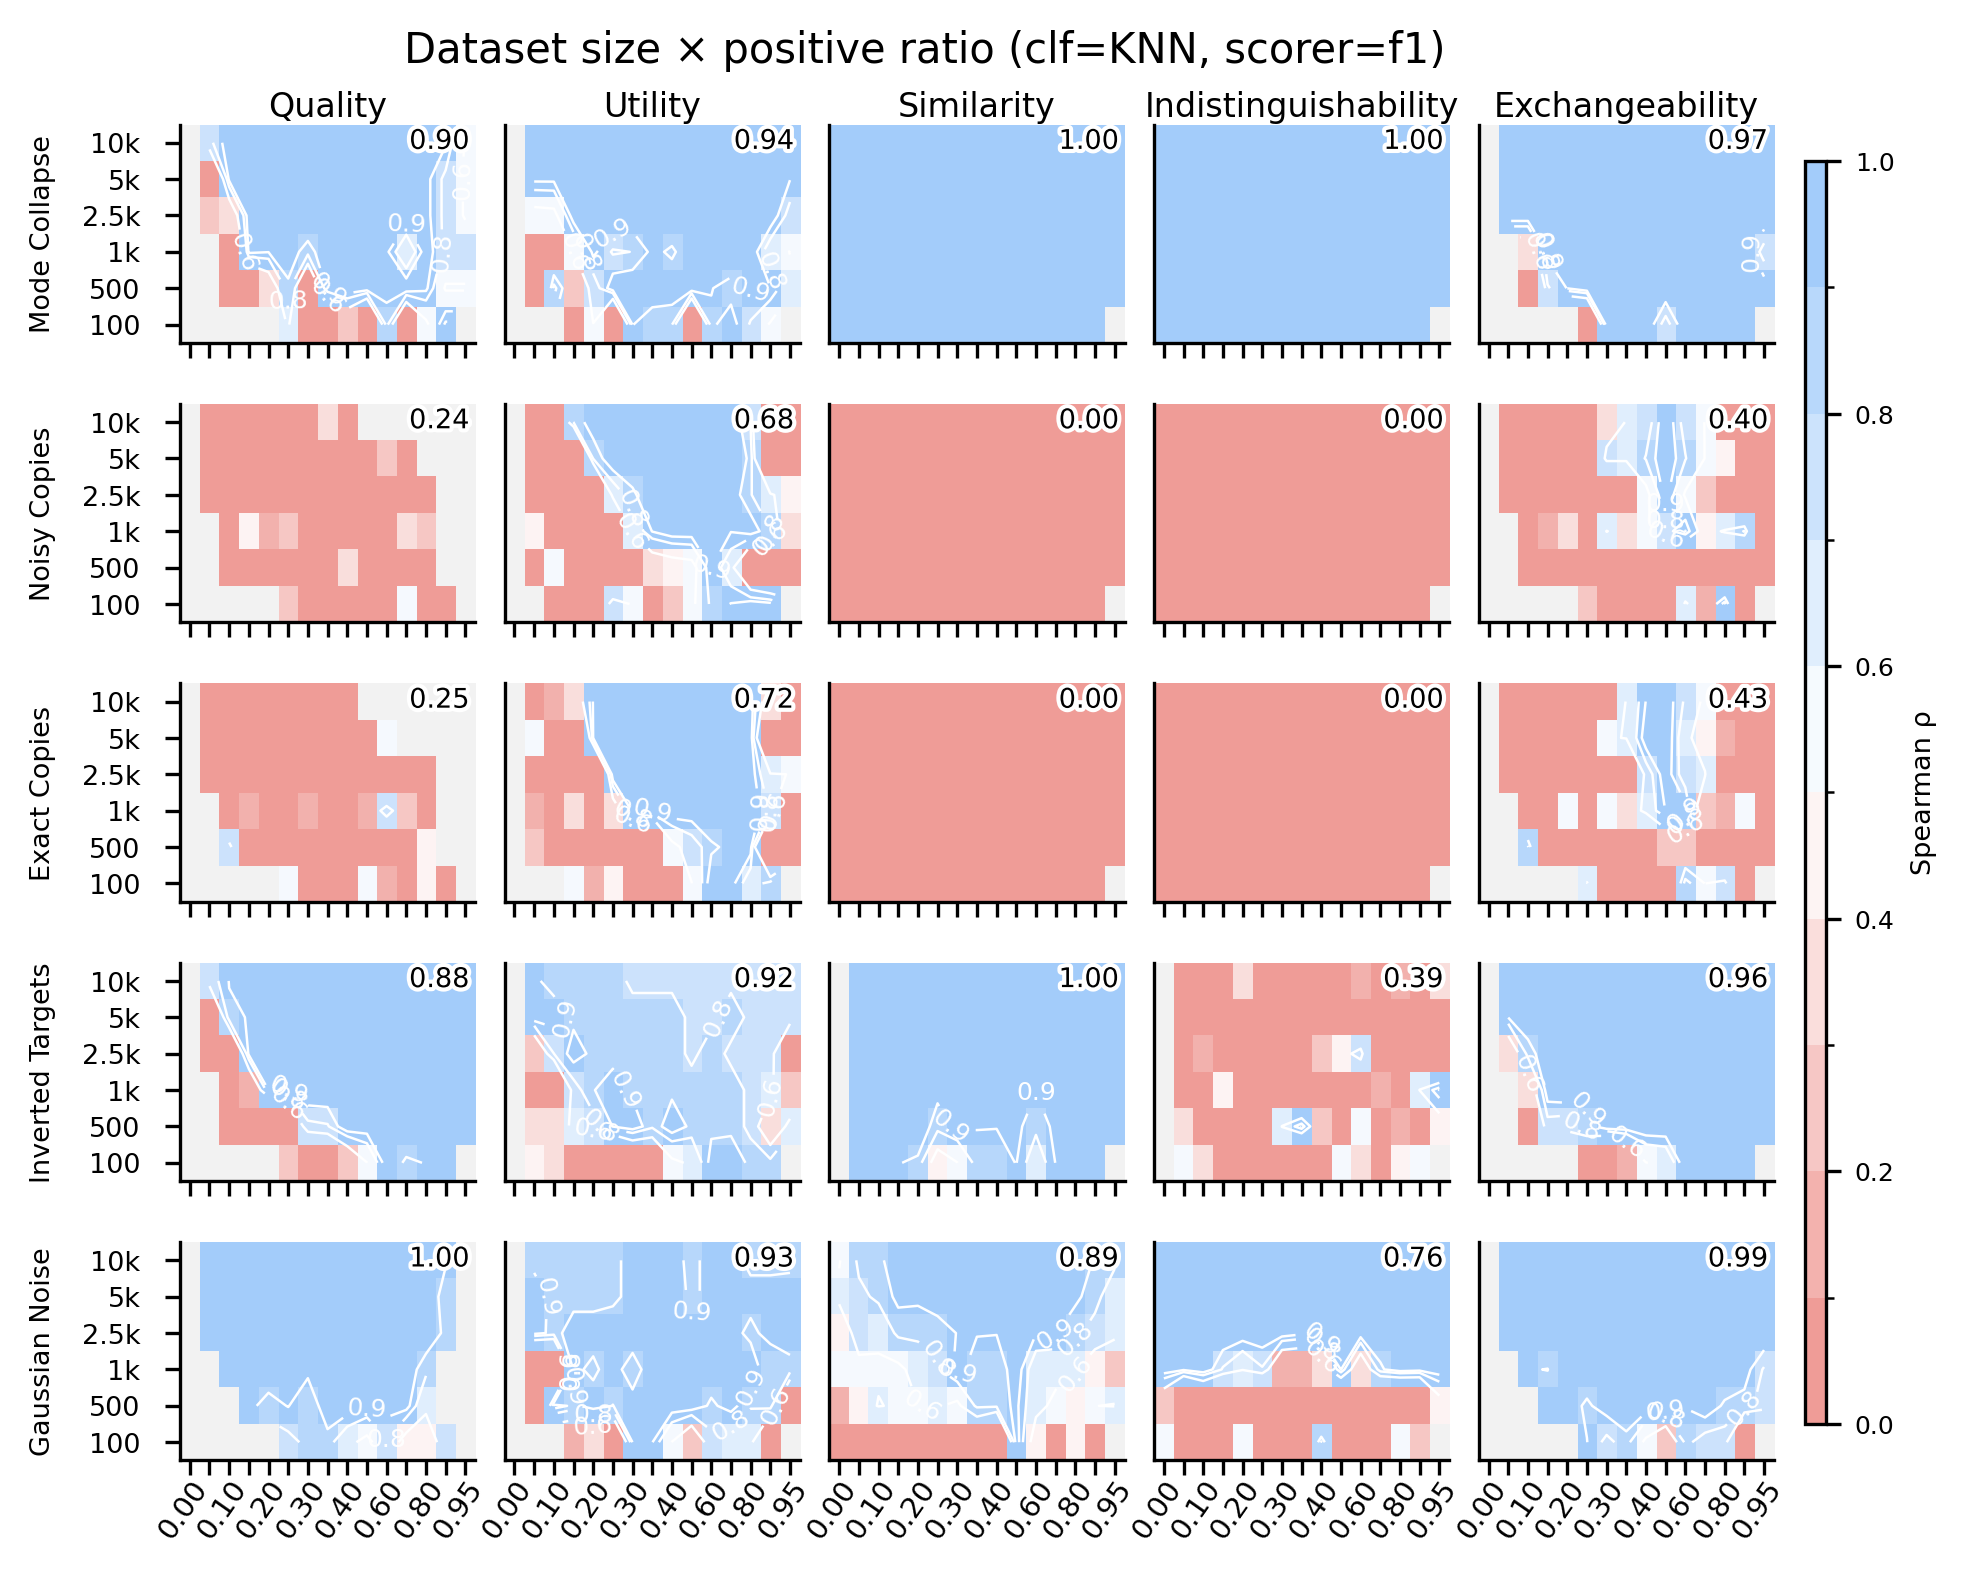
\includegraphics[width=\linewidth]{images/rankgen/synthetic/size_vs_pos.png}% don't set height; keepaspectratio is default
  \caption[Stability maps: size × positive ratio]{Stability maps for \emph{dataset size × positive ratio}
  (clf=KNN, scorer=f1). Color shows Spearman’s $\rho$ (clipped to $[0,1]$); the
  number in each panel is $\widehat{p}_{\mathrm{deg}}=\Pr(\rho>0)$, the fraction of
  grid settings that degrade (smaller is better).}
  \label{fig:size-vs-pos}
\end{figure}

\textbf{Diagnosing Generators via Metric Profiles.}
Figure~\ref{fig:size-vs-pos} illustrates how each quantile-estimated RankGen metric responds to different perturbation types and dataset sizes.
Beyond canonical failure modes, we introduce a novel scenario—\emph{noisy copies}—in which near-duplicates of training samples, lightly corrupted with Gaussian noise, are injected into the generated set.
This case is particularly valuable for testing sensitivity to memorisation.

Each metric offers a distinct diagnostic signal, effectively fingerprinting how a generator fails.
\textbf{Quality} sharply degrades under mode collapse, label flips, and Gaussian noise—revealing poor generalisation.
\textbf{Utility} uniquely detects memorisation in the noisy-copy scenario and remains robust across most perturbations.
\textbf{Indistinguishability} is highly sensitive to global shifts and feature corruption but fails to flag copying, where the discriminator underfits.
\textbf{Similarity} captures structural misalignment from label and topology noise, though it too struggles with near-copies.
\textbf{Exchangeability} synthesizes these perspectives into a single, composite view—capturing both task-relevance and distributional alignment.
However, as a consequence of this blending, its behaviour can become non-monotonic in edge cases.
In the noisy-copy setting, for example, utility steadily declines as duplication increases, while similarity paradoxically improves—since noisy copies still resemble the original data.
When these two effects compete, Exchangeability can appear erratic, exposing a tension between structural proximity and task degradation.

\textbf{Comparison with Baseline Metrics.}
As shown in Appendix \ref{appendix:pr_dc}, we also evaluate Coverage/Density~\citep{kynkaanniemi2019improved},
Precision/Recall for distributions~\citep{sajjadi2018assessing},
FID~\citep{heusel2017gans},
MMD (Linear/RBF)~\citep{gretton2012kernel},
and F1-based variants~\citep{powers2011f1}.
While some of these exhibit strong correlations under specific perturbations (e.g., \textbf{F1\_PR} under mode collapse, or \textbf{MMD} under Gaussian noise), their overall sensitivity is limited.
\subsubsection{\textbf{How often classifiers may fail the PAC Bounds}}
Across all synthetic perturbation experiments, Table~\ref{tab:pac-fail-overall} reports how frequently classifier probes failed to satisfy their PAC bounds at $\delta = 0.05$. Failures are relatively rare for tree-based methods (e.g., Random Forests, Gradient Boosting, AdaBoost), which almost always produced statistically reliable estimates across axes. In contrast, some simple classifiers show much higher failure rates: GaussianNB and Logistic Regression violated bounds nearly half the time on the \emph{Utility} and \emph{Exchangeability} axes, while SVC and $k$-NN occasionally failed on \emph{Quality}. These differences highlight that not all classifiers provide equally stable probes. The overall pattern reinforces the value of PAC-style guarantees: they make explicit when a probe’s conclusions are statistically trustworthy, and when they should be treated with caution.
\normalsize
\begin{table}[H]
  \centering
  \footnotesize
  \setlength{\tabcolsep}{3.5pt}
  \renewcommand{\arraystretch}{1.15}
  \begin{tabularx}{\columnwidth}{l *{5}{r}}
    \toprule
    {\textbf{Classifier}} &
    {\makecell{\textbf{Quality}}} &
    {\makecell{\textbf{Utility}}} &
    {\makecell{\textbf{Indistinguishability}}} &
    {\makecell{\textbf{Similarity}}} &
    {\makecell{\textbf{Exchangeability}}} \\
    \midrule
    AdaBoostClassifier         & 0.000 & 0.167 & 0.067 & 0.000 & 0.167 \\
    DecisionTreeClassifier     & 0.006 & 0.167 & 0.042 & 0.000 & 0.167 \\
    ExtraTreesClassifier       & 0.048 & 0.167 & 0.194 & 0.000 & 0.167 \\
    GaussianNB                 & 0.273 & 0.500 & 0.064 & 0.000 & 0.500 \\
    GradientBoostingClassifier & 0.027 & 0.167 & 0.085 & 0.000 & 0.167 \\
    KNeighborsClassifier       & 0.145 & 0.000 & 0.033 & 0.000 & 0.000 \\
    LogisticRegression         & 0.161 & 0.482 & 0.030 & 0.000 & 0.482 \\
    RandomForestClassifier     & 0.048 & 0.167 & 0.124 & 0.000 & 0.167 \\
    SVC                        & 0.215 & 0.000 & 0.048 & 0.000 & 0.000 \\
    \bottomrule
  \end{tabularx}
  \caption{Overall PAC \emph{fail frequency} (proportion) by classifier, aggregated across all synthetic experiments at $\delta=0.05$ (lower is better).}
  \label{tab:pac-fail-overall}
\end{table}

\subsubsection{\textbf{PCA of RankGen Metrics on Synthetic Perturbations}}
\label{sec:pca-synthetic}
\begin{figure}[H]
  \centering
  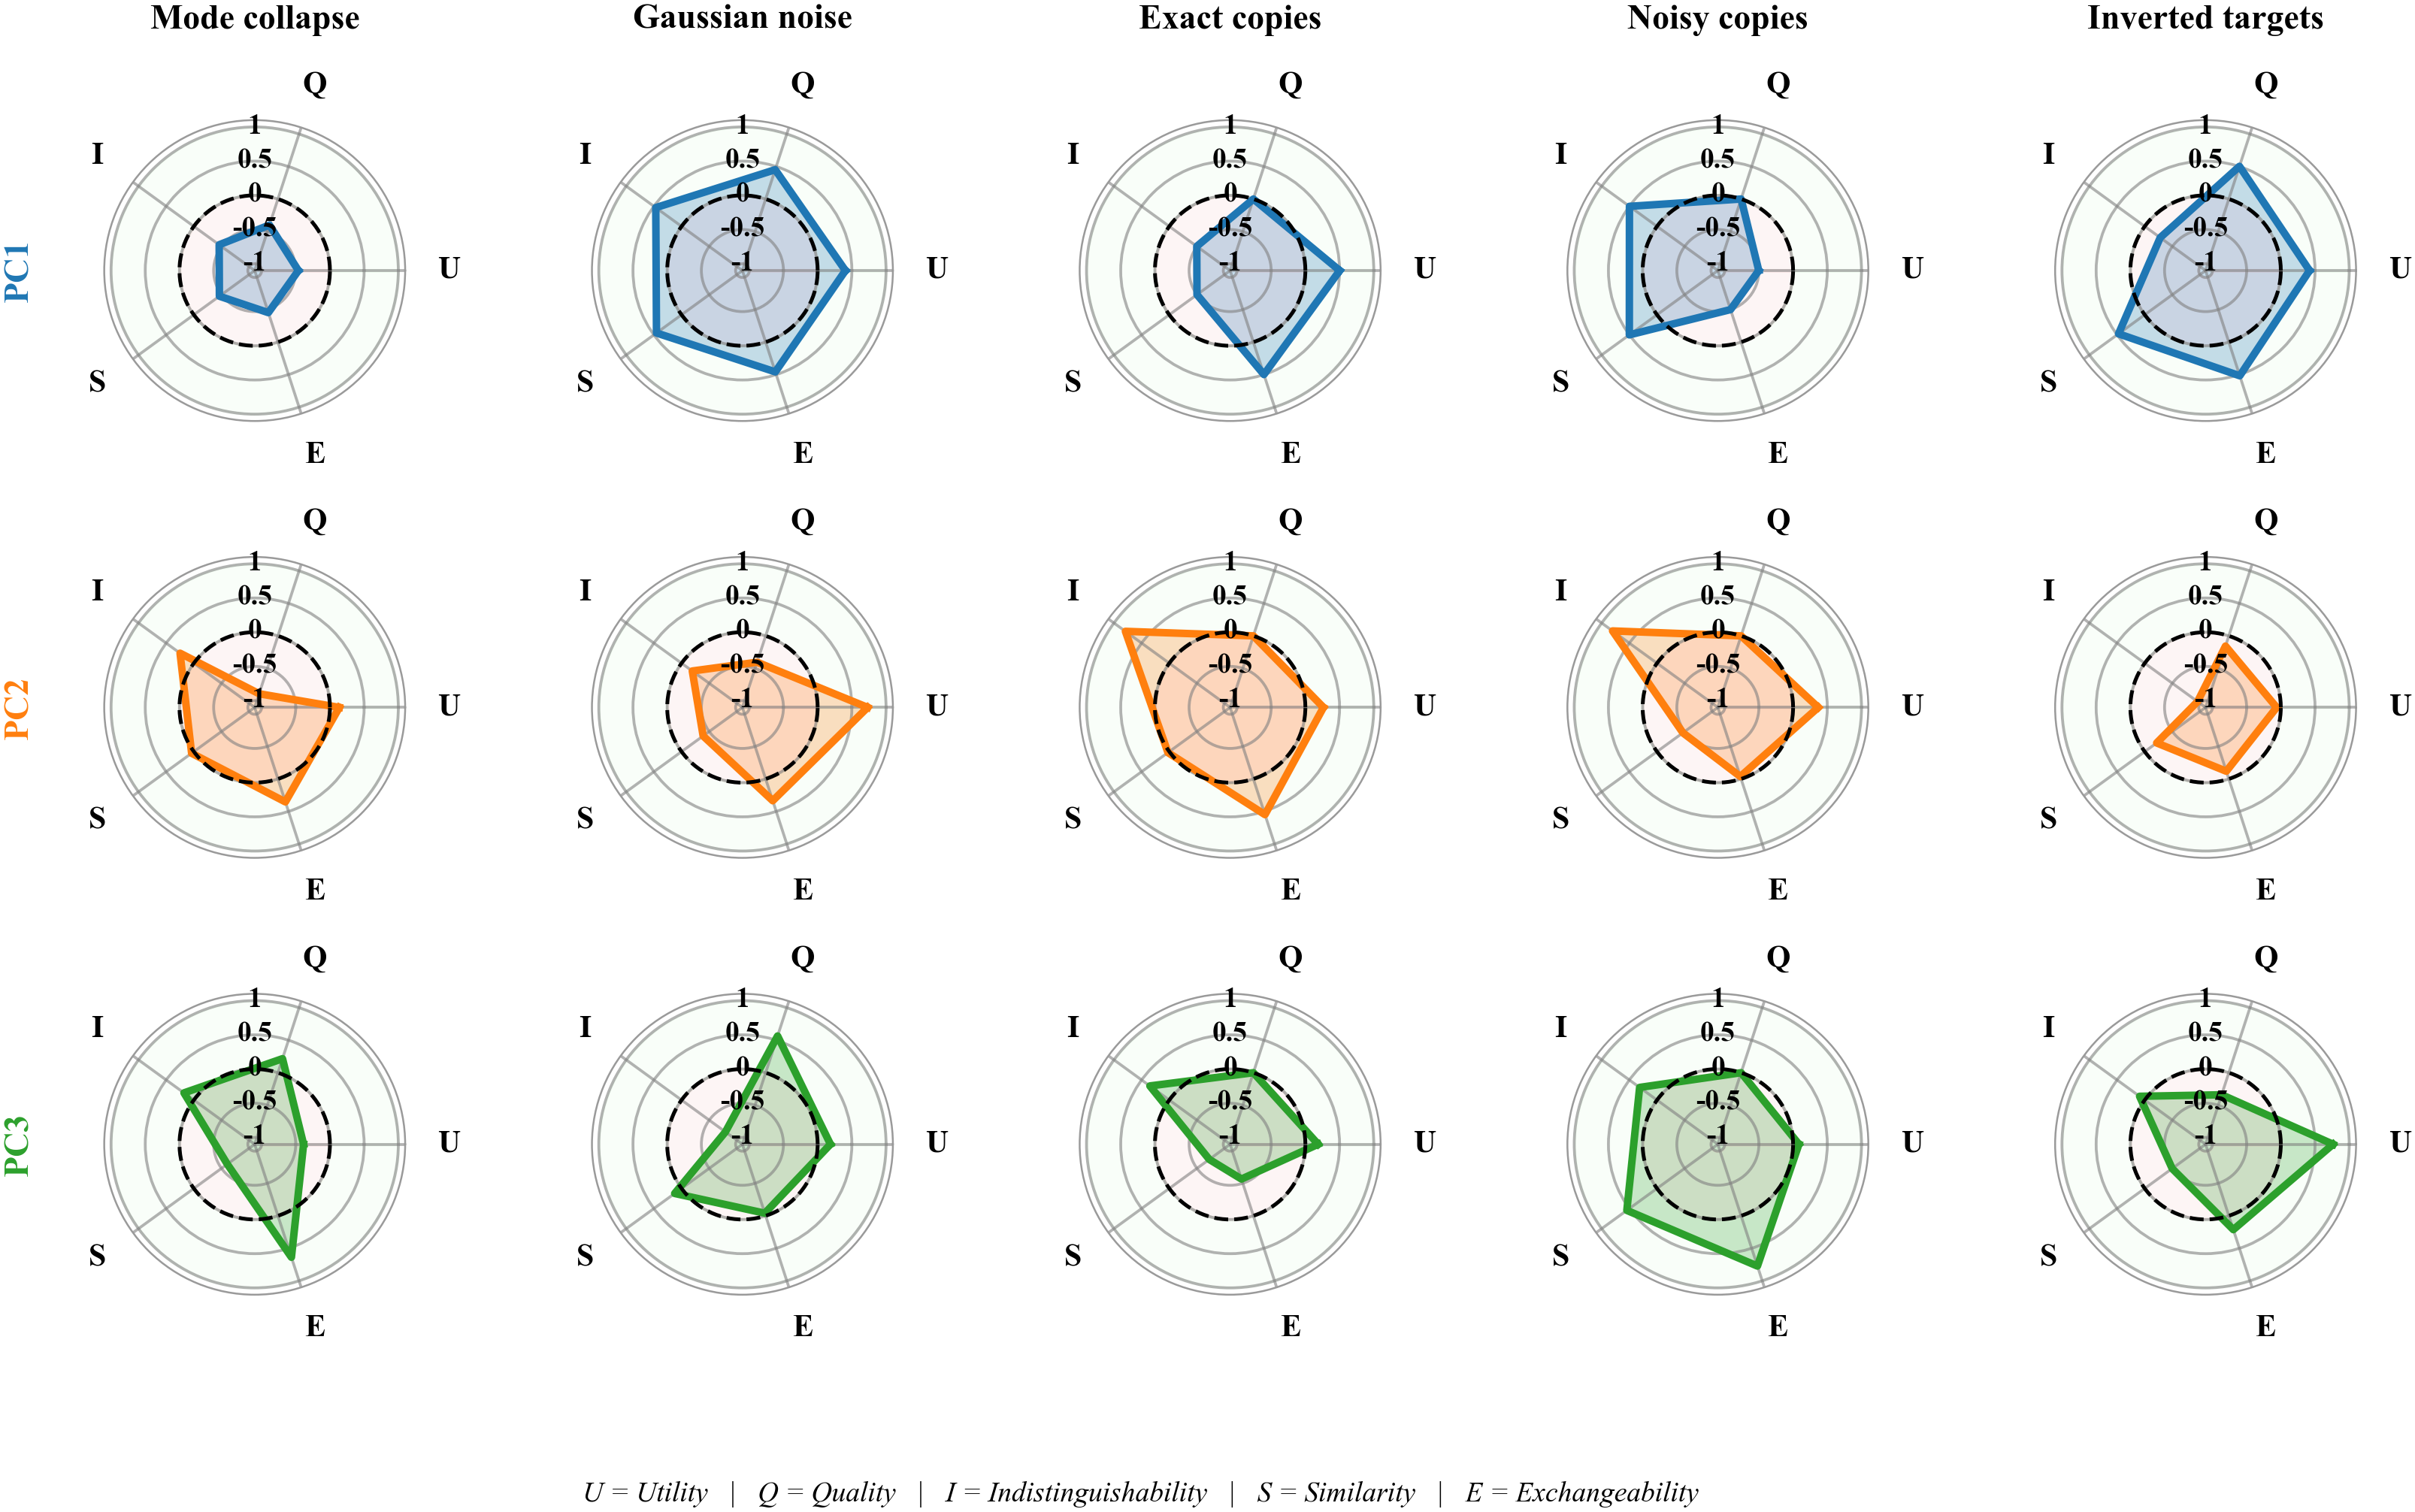
\includegraphics[width=1\linewidth]{images/rankgen/synthetic/radial_plot.png}
  \caption{\textbf{PCA loadings of RankGen metrics under synthetic perturbations.}
  Columns correspond to perturbations (Mode collapse, Gaussian noise, Exact copies, Noisy copies, Inverted targets).
  Rows correspond to principal components (PC1–PC3), color-coded by PC (blue = PC1, orange = PC2, green = PC3).
  Each radar plot shows loadings of $\{U,Q,I,S,\mathcal E_{\min}\}$; the dashed circle marks $0$ (rings at $\pm0.5$ and $\pm1$).
  PC1 captures a global corruption factor, while PC2/PC3 reveal complementary trade-offs (e.g., $Q$ vs.\ $I/E$, or $U$ vs.\ $S$).}
\end{figure}
We apply PCA to standardized metric vectors $(U,Q,I,S,E)$ to study how RankGen’s axes co-vary under canonical perturbations. Standardization (zero mean, unit variance) ensures that principal components reflect \emph{shared structure} rather than differences in raw scale \citep{jolliffe2002pca,abdi2010pca}.

\paragraph{Global factor vs.\ structured trade-offs.}
Across most perturbations, \textbf{PC1} behaves as a global “level” factor: all metrics load in the same direction, capturing overall corruption severity. This pattern is clearest in the Gaussian noise and mode collapse settings, where PC1 explains nearly all variance with uniform contributions from $\{U,Q,I,S,E\}$. By contrast, perturbations involving duplication or label inversion distribute variance across multiple components. In noisy copies and inverted targets, PC1 accounts for a smaller share, leaving PC2/PC3 to isolate distinct residual signals.

\paragraph{Scenario-specific axes.}
The remaining components (PC2, PC3) disentangle complementary trade-offs. For Gaussian noise, PC2 contrasts \textbf{Quality} against \textbf{Indistinguishability} and \textbf{Exchangeability}, while PC3 highlights residual variance in \textbf{Utility}. For mode collapse, PC2/PC3 emphasise losses in \textbf{Similarity} and \textbf{Utility}, consistent with reduced local mixing and predictive value. For exact copies, higher-order axes distinguish between inflated \textbf{Indistinguishability} and depressed \textbf{Utility}/\textbf{Similarity}, reflecting the fact that duplicates look realistic but add little value. In noisy copies, the decomposition shows a more complex balance, with \textbf{Quality} and \textbf{Exchangeability} trading off against \textbf{Similarity}. Finally, in inverted targets, PC2 is dominated by \textbf{Indistinguishability}, while PC3 sets \textbf{Utility} against \textbf{Similarity} and \textbf{Quality}, consistent with models that flip labels being easy to tell apart yet still producing plausible-looking samples.

\paragraph{Interpretation.}
Signs of loadings are arbitrary in PCA \citep{abdi2010pca,lever2017pca}; what matters are their relative magnitudes and oppositions. The fact that PC2/PC3 consistently recover orthogonal axes beyond the global level confirms that RankGen’s metrics are not collinear. Instead, they capture complementary error signatures: once the “common factor” is removed, residual axes reveal whether degradation arises from poor utility, collapsed similarity, or label inversion. This diagnostic separation is precisely what RankGen is designed to provide.



\subsection{Real-World Graph Datasets}
\label{sec:real-world-graphs}
We focus our real-world evaluation on structured domains where human inspection is infeasible—
specifically, molecular graphs. Unlike images, where qualitative assessment is often possible, graphs lack intuitive visual cues, making rigorous, task-relevant evaluation metrics essential. To reflect realistic deployment scenarios where human curation or large-scale pretraining is not viable, we train generative models on relatively small datasets (hundreds to a few thousand instances), simulating low-resource settings common to several scientific domains.

Our datasets are sourced from the \textit{Therapeutics Data Commons}\citep{huang2021tdc}, encompassing a diverse suite of molecular prediction tasks relevant to drug discovery and pharmacology: \textsc{AMES} (mutagenicity prediction), \textsc{BBB} (blood–brain barrier penetration), \textsc{CYP1A2} and \textsc{CYP2C19} (cytochrome P450 enzyme binding), \textsc{hERG} (cardiotoxicity risk via hERG channel inhibition), and \textsc{Lipophilicity} (logP estimation as a proxy for solubility and absorption). Each molecule is originally provided as a SMILES string\citep{weininger1988smiles}, which we convert into graph representations where atoms are nodes and bonds are edges.
\begin{figure}[H]
  \centering
   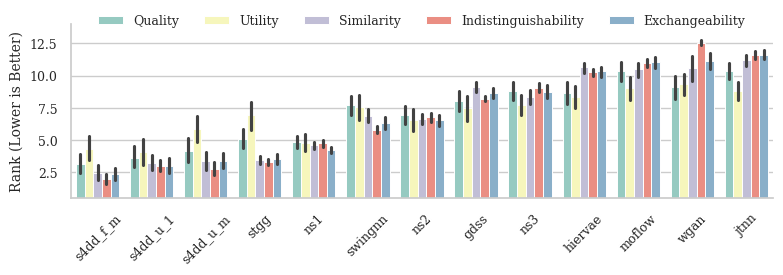
\includegraphics[width=\textwidth]{images/rankgen/real_generators/generators_rank_all_datasets.png}
  \caption{Average generator rank per metric across all datasets and vectorizers. Lower is better.}
  \label{fig:generators-rank}
\end{figure}
For each dataset, we perform class-conditional generation using a diverse set of molecular generative models spanning multiple paradigms. \textbf{STGG}\citep{ahn2021spanning} is an autoregressive model that constructs molecules via spanning trees; \textbf{WGAN-GP with R-GCN}\citep{keras2021wgan} applies adversarial training to graph-structured data; \textbf{JTNN}\citep{jin2018junction} and \textbf{HierVAE}\citep{c} are hierarchical variational autoencoders, the former based on junction trees and the latter on motif assembly; \textbf{MoFlow}\citep{zang2020moflow} is a normalizing flow model allowing exact likelihood estimation; \textbf{GDSS}\citep{jo2022score} is a score-based diffusion model built on stochastic differential equations; and \textbf{SWINGNN}\citep{yan2023swingnn} is a graph diffusion model enhanced with shifted window attention. We also introduce the \textbf{Neighborhood Swap Generator (NS)}, a non-parametric, training-free method that perturbs input graphs through iterative local rewiring of neighbourhood subgraphs, producing diverse synthetic variants across one to three rounds of compounding perturbations (NS-1, NS-2, NS-3). These models collectively span autoencoding, flow-based, adversarial, diffusion-based, and perturbation-based generative paradigms (see Appendix~\ref{appendix:molecular_datasets} and Appendix~\ref{appendix:hyperparameters_for_molecular} for details).

\textbf{Feature Representation.}
To enable consistent comparison, we convert molecular graphs into fixed-length vectors using three types of encoders: (1) classical fingerprints (e.g., \textbf{Morgan}, \textbf{Torsion}, \textbf{Atom Pair}, \textbf{RDKit}\citep{rdkit2011}); (2) neural graph embeddings from models such as \textbf{GIN}\citep{xu2019powerful}, \textbf{GraphCL}\citep{you2020graph}, and \textbf{InfoGraph}\citep{sun2019infograph}; and (3) discrete graph kernels, notably \textbf{NSPDK}~\citep{costa2010fast}. This diversity supports robust evaluation across both learned and handcrafted feature spaces. While overall trends are consistent, we observe that the choice of vectorizer can influence generator rankings within each PAC-valid group, highlighting the importance of feature representation in shaping performance signals.
\paragraph{Model Comparison Across Real Generators.}
Figure~\ref{fig:generators-rank} displays the average quantile-based ranking of each generator, aggregated across datasets and feature encodings.\footnote{Table~\ref{tab:bounds_check} reflects a single experimental run (see Fig.\ref{fig:rank_herg_karim}), while Fig.\ref{fig:generators-rank} averages over multiple trials—accounting for observed differences.} \textbf{S4DD} variants and \textbf{STGG} consistently achieve top rankings across all metrics, indicating strong generalisation and distributional alignment. In contrast, models such as \textbf{WGAN} and \textbf{MoFlow} rank poorly—particularly in \textbf{Exchangeability}—suggesting limited task utility and diversity.
Interestingly, the pretrained version of S4DD—trained on over a million molecules—does not yield substantial gains over its dataset-specific counterparts trained on only a few thousand examples. This suggests that broad pretraining does not necessarily translate into better generative performance under task-specific constraints.
These findings reinforce RankGen’s central insight: matching superficial distributional statistics is not enough. While some models may inflate conventional metrics through memorisation, \textbf{Exchangeability} penalizes such behaviour by jointly evaluating utility and alignment—providing a more trustworthy, single-score summary for model selection.


\subsection{Image Benchmarks: MNIST, Fashion--MNIST, and CIFAR--10}
\label{sec:image-benchmarks}
\begin{figure}[H]
  \centering
  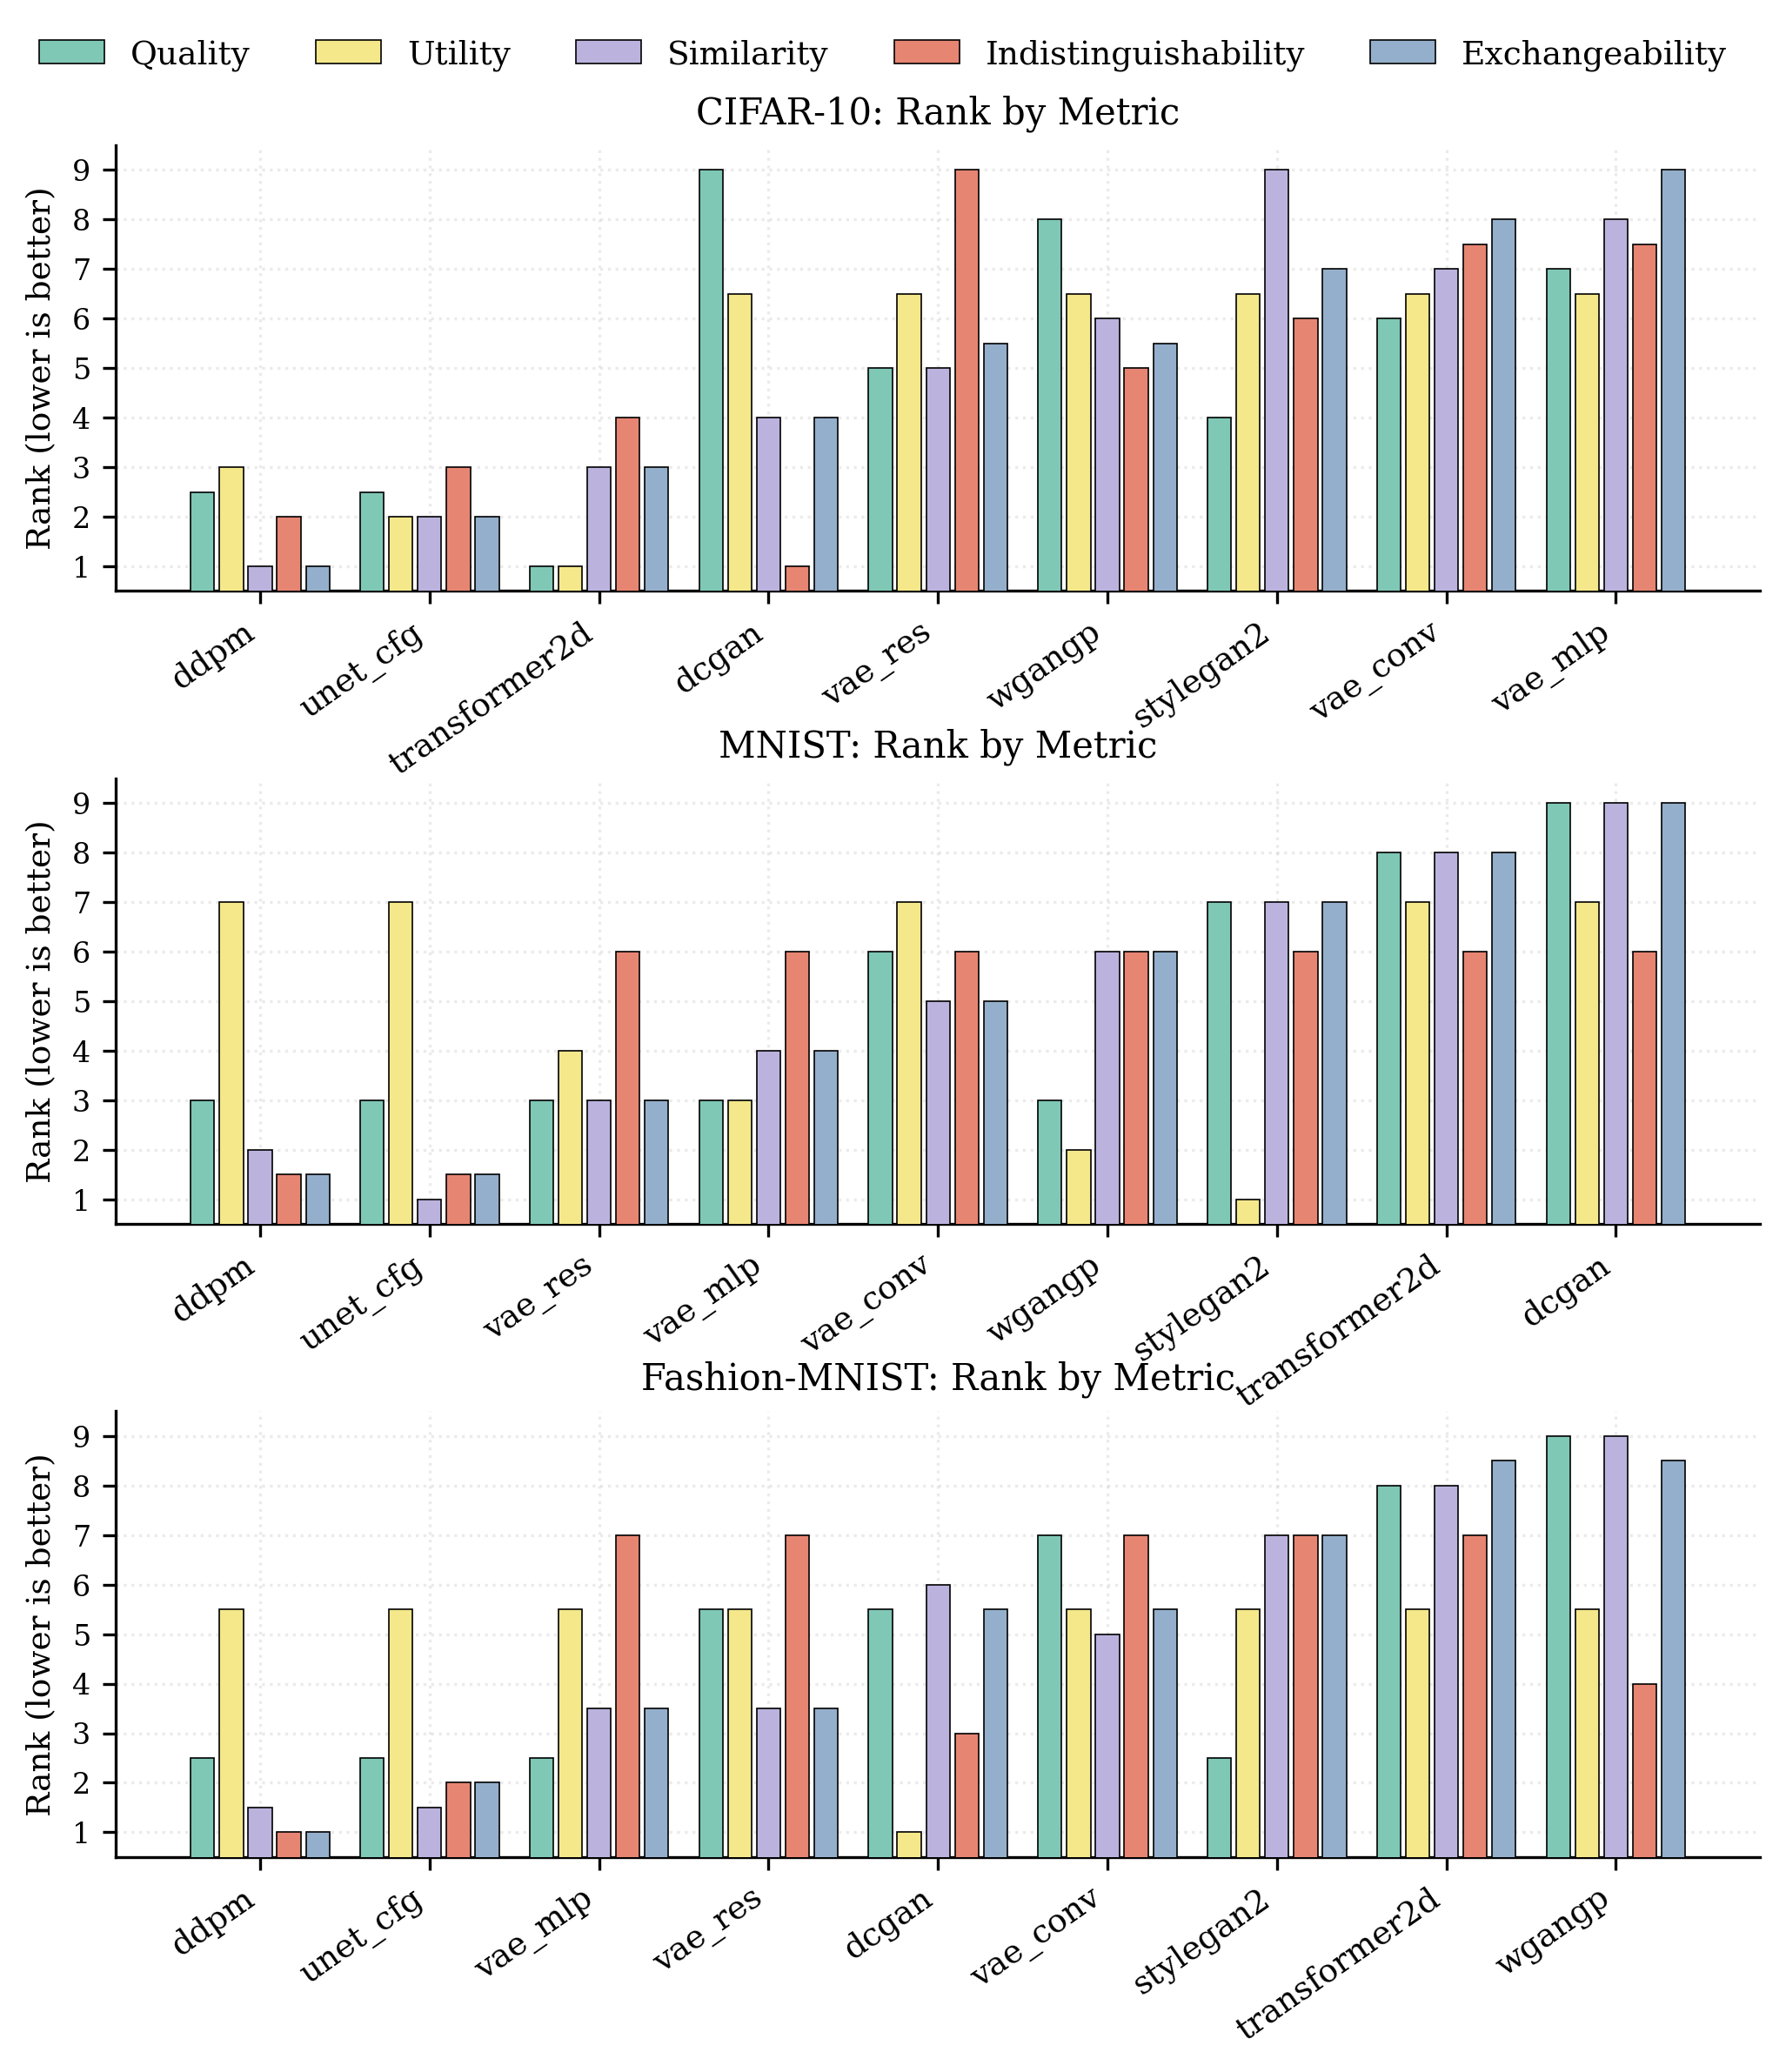
\includegraphics[width=0.80\linewidth,height=1.5\textheight,keepaspectratio]{images/rankgen/real_generators/rank_images.png}
  \caption{RankGen ranks on \textbf{CIFAR--10}, \textbf{MNIST}, and \textbf{Fashion--MNIST}.
  Lower is better. StyleGAN2-lite exhibits high Quality but low Utility and Similarity, echoing our synthetic mode-collapse setting. This suggests strong precision but poor coverage—models of this type risk overfitting narrow regions of the data. VAEs remain competitive on digits.}
  \label{fig:cifar10-ranks}
\end{figure}
We use three canonical benchmarks: \textbf{MNIST}~\citep{lecun1998gradient},
\textbf{Fashion--MNIST}~\citep{xiao2017fashion}, and \textbf{CIFAR--10}~\citep{krizhevsky2009learning},
with consistent preprocessing and stratified splits (Appendix~\ref{app:image-experiments}).
Test images are never used for training or selection. We evaluate class-conditional generators spanning multiple paradigms.
\textbf{VAEs:} MLP-VAE, Conv-VAE, and ResNet-VAE~\citep{kingma2014auto,rezende2014stochastic}.
\textbf{GANs:} DCGAN~\citep{radford2016unsupervised}, WGAN--GP with projection discriminator~\citep{gulrajani2017improved,miyato2018cgans}, and a $32{\times}32$ \textbf{StyleGAN2-lite}~\citep{karras2020analyzing}.
\textbf{Diffusion:} cDDPM with UNet backbone~\citep{ho2020denoising,ronneberger2015u,ho2022classifier} and a Transformer2D backbone (DiT style)~\citep{peebles2023di}, using HuggingFace Diffusers samplers~\citep{von-platen-etal-2022-diffusers} (see architectural and training details  in Appendix~\ref{app:image-models}).
\paragraph{RankGen summary and diagnostics.}
Figure~\ref{fig:cifar10-ranks} summarizes generator \emph{ranks} under RankGen
(Quality $Q$, Utility $U$, Indistinguishability $I$, Similarity $S$, and Exchangeability $E$)
across datasets. Several consistent patterns emerge.

\textit{First}, diffusion models are the only family that consistently balances all four base metrics,
achieving strong overall Exchangeability. They dominate $Q$ and $S$ across datasets, reflecting high visual fidelity
and broad distributional coverage, which is also evident in the sample panels.

\textit{Second}, GAN-based models exhibit clear trade-offs.
\texttt{stylegan2} attains high $Q$ but shows weak $U$ and $S$, consistent with a high-precision/low-recall regime
characteristic of mode collapse: samples are sharp but lack diversity and task utility.
Conversely, \texttt{dcgan} achieves strong $I$ while remaining near chance in $U$, indicating that although samples may appear realistic,
they provide limited augmentation value. These patterns highlight how single-number heuristics (e.g., IS)
can obscure important failure modes.

\textit{Third}, VAEs underperform on CIFAR--10 due to reduced $Q$ and $U$, reflecting blur and limited diversity,
but remain competitive on MNIST and Fashion--MNIST, where lower complexity and grayscale structure better match their inductive bias.

Overall, RankGen reveals distinct architectural ``fingerprints'', diagnosing failure modes that are otherwise flattened by aggregate scores.
The underlying metric values are reported in Appendix~\ref{app:image-results}, with illustrative samples shown in
Figures~\ref{fig:cifar10_generated_panel}, \ref{fig:fashionmnist_generated_panel}, and \ref{fig:mnist_generated_panel}
(Appendix~\ref{appendix:example}).
We further compare RankGen to standard metrics such as FID, KID, PRD, and VENDI
(Tables~\ref{tab:vals-ranks-cifar10}--\ref{tab:ke-mnist-ranked}), observing broad agreement in well-behaved regimes
(e.g., diffusion models ranking highest), alongside informative divergences in settings where classical metrics are known to be less reliable.


\subsection{RankGen and Conventional Image Metrics}
\label{sec:rankgen-vs-conventional}

To contextualize the RankGen scores, we compare them against standard image
evaluation metrics and kernel--entropy diversity proxies. Figure~\ref{fig:mnist-ranks}
reports Spearman correlations between per-generator ranks under RankGen and
under conventional image metrics, while the full numeric results are deferred to
Appendix~\ref{app:image-results}.

\paragraph{Conventional image metrics.}
We report FID~\citep{heusel2017gans}, KID~\citep{binkowski2018demystifying},
precision/recall for distributions and their harmonic mean
(\textbf{F1\_pr})~\citep{sajjadi2018assessing,kynkaanniemi2019improved}, and
Inception Score (IS)~\citep{salimans2016improved}, using
$n_{\text{ref}}=n_{\text{gen}}$ as indicated. Across datasets, diffusion models
(\texttt{ddpm}, \texttt{unet\_cfg}) achieve the best or near-best FID/KID and
the strongest F1\_pr, while \texttt{stylegan2} exhibits high precision but very
low recall, consistent with mode dropping. VAEs underperform on CIFAR--10 but
remain more competitive on MNIST and Fashion--MNIST. Full results with
per-metric ranks are reported in
Tables~\ref{tab:cifar10-ranked}--\ref{tab:mnist-ranked}.

\paragraph{Kernel--entropy diversity proxies.}
To complement embedding-based distances, we also compute kernel--entropy
proxies of sample diversity: VENDI/RKE surrogates estimated via FKEA
(RKE\_gen, FKEA--VENDI\_gen, FKEA--RKE2\_gen) and the reference-relative
variant RRKE (lower is better)~\citep{friedman2023vendi,pasarkar2024cousins,jalali2024fkea,luo2024converge}.
Per-dataset results and kernel widths $\sigma$ are given in
Tables~\ref{tab:ke-cifar10-ranked}--\ref{tab:ke-mnist-ranked}. Diffusion models
again rank highest, showing higher entropy and lower redundancy, while VAEs
show reduced entropy and GANs occupy an intermediate regime. As discussed in
Sec.~\ref{sec:related:evaluation}, these spectral scores are useful for
detecting mode collapse, but they remain label- and task-agnostic and operate
primarily on the generated set, so they cannot by themselves diagnose copying
or augmentation value.

\paragraph{Relationship to RankGen.}
Figure~\ref{fig:mnist-ranks} shows that RankGen is broadly consistent with
conventional metrics where expected, but provides additional diagnostic
resolution. In particular, RankGen $Q$ and $S$ align closely with precision and
recall, while exchangeability $\mathcal{E}_{\min}$ aligns most strongly with
$F1_{\text{pr}}$, indicating that the composite captures both fidelity and
coverage. By contrast, IS exhibits weaker and less consistent agreement. This
agreement is strongest on MNIST, but remains qualitatively stable across all
three datasets.

The key advantage of RankGen appears precisely in the cases where conventional
metrics disagree or become ambiguous. Diffusion models rank near the top under
both metric families, but models such as StyleGAN2 and WGAN--GP reveal the
added value of RankGen’s task-aware probes. StyleGAN2 achieves competitive
FID/KID and high precision, yet RankGen assigns it low Utility and low
Similarity, exposing its concentrated, mode-dropping behaviour. WGAN--GP
obtains middling conventional scores, but RankGen identifies near-zero Utility,
indicating that its samples add little task-relevant information despite
appearing plausible in feature space. Likewise, VAEs may remain moderately
ranked by FID/KID on simpler datasets, but RankGen exposes their weaker task
fidelity and augmentation value, especially on CIFAR--10.

Overall, conventional metrics capture global similarity and diversity, whereas
RankGen additionally measures task fidelity, augmentation value, local mixing,
and copying sensitivity. The two families are therefore best viewed as
complementary: conventional metrics provide broad distributional summaries,
while RankGen explains \emph{why} generators with similar global scores can
behave very differently in downstream use.

\begin{figure}[H]
  \centering
  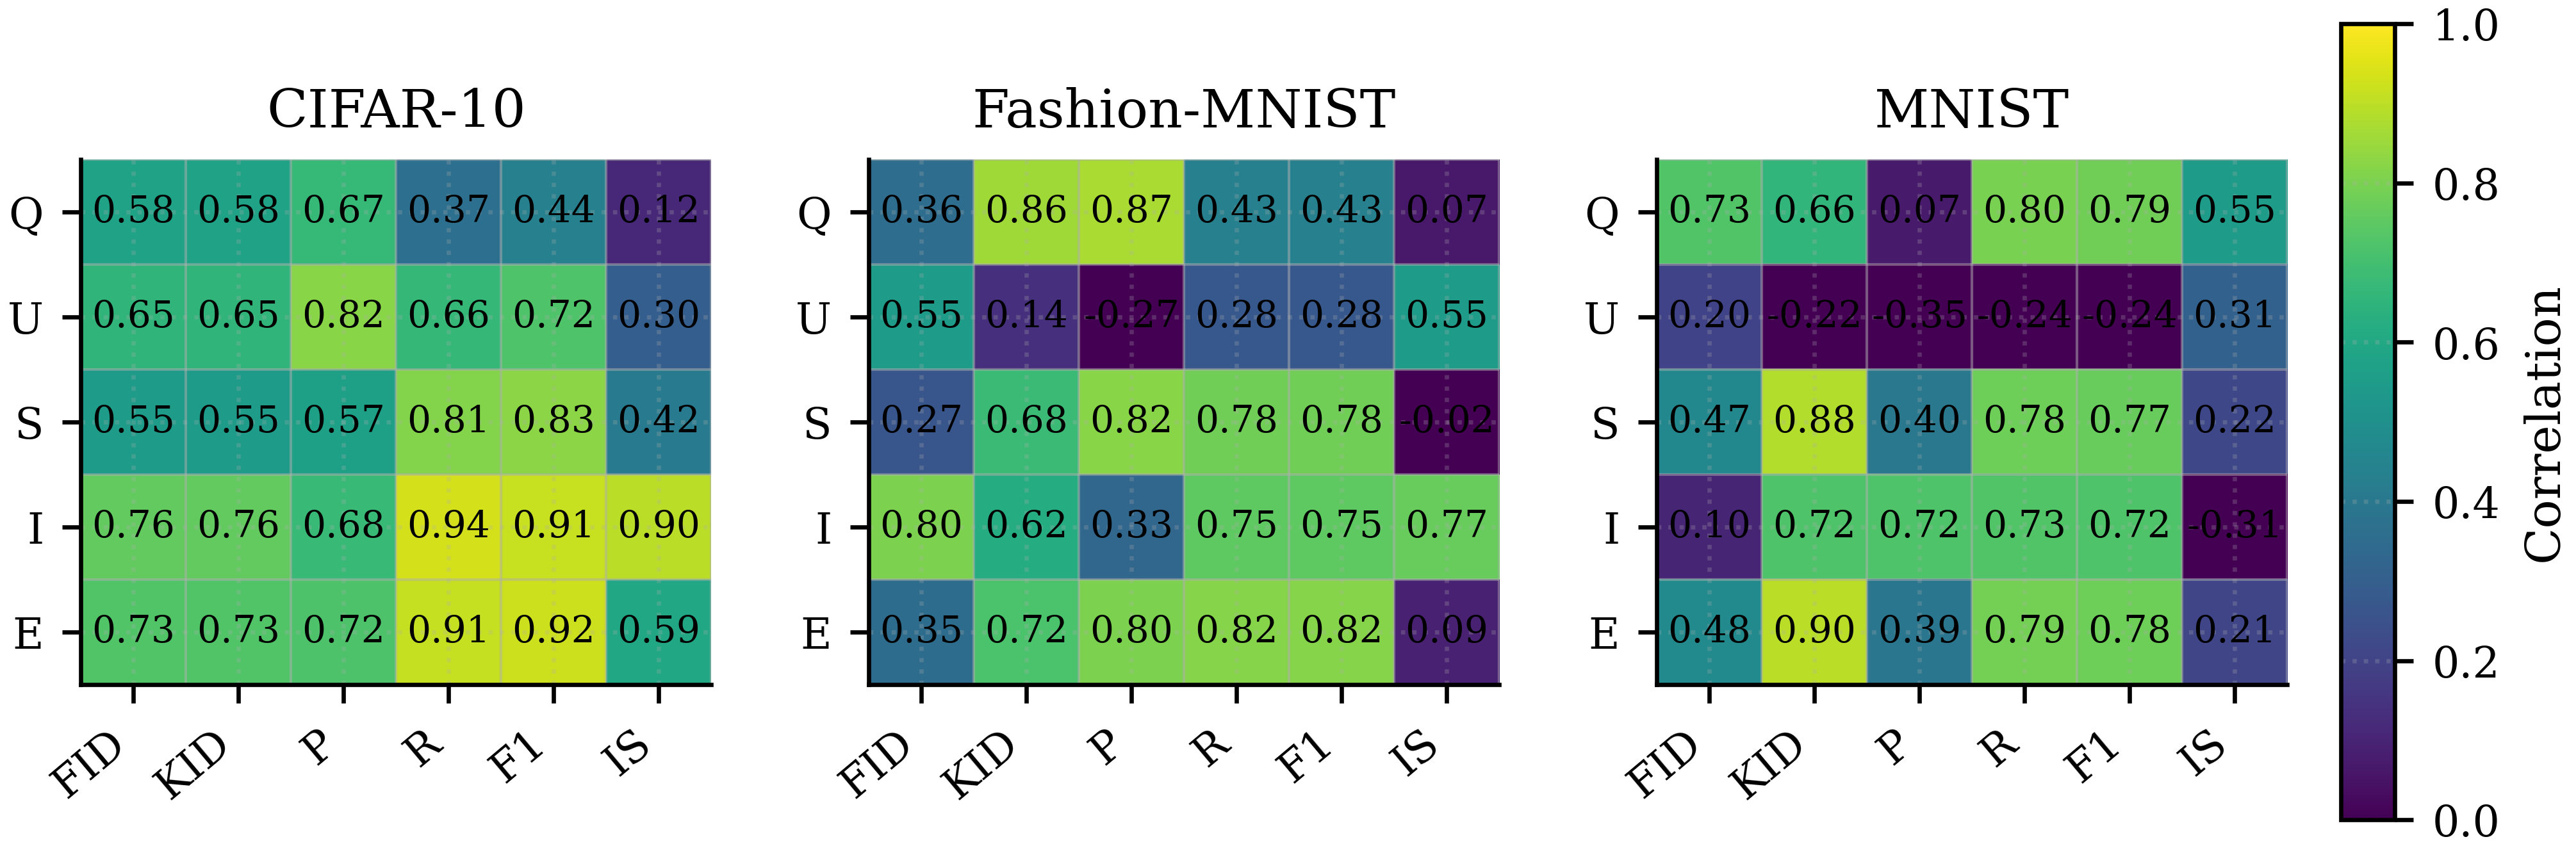
\includegraphics[width=\linewidth,height=0.82\textheight,keepaspectratio]{images/rankgen/real_generators/rank_corr_3panel.png}
  \caption{\textbf{RankGen vs.\ conventional metrics (by dataset).}
  Cells show Spearman correlations between RankGen metrics
  ($Q,U,S,I,\mathcal{E}_{\min}$) and conventional metrics
  (FID, KID, P, R, $F_{1,\mathrm{pr}}$, IS) on \textbf{CIFAR--10},
  \textbf{Fashion--MNIST}, and \textbf{MNIST}. RankGen $Q$ and $S$ track
  precision and recall, while exchangeability aligns most closely with
  $F_1$. IS shows the weakest alignment.}
  \label{fig:mnist-ranks}
\end{figure}
\subsection{Open-Domain Text Generation}
\label{subsec:text}

To assess whether \textsc{RankGen} generalises beyond graph and image generators, we evaluate it on open-domain text generation using the \textsc{AG-News} corpus~\citep{zhang2015character}, which contains news headlines labelled with four topics (\emph{World}, \emph{Sports}, \emph{Business}, \emph{Sci/Tech}). We treat human-written headlines as real data and consider three GPT-2 variants~\citep{radford2019language} as conditional generators: \texttt{distilgpt2}, \texttt{gpt2}, and \texttt{gpt2-medium}. For each class, models are prompted with a topic-specific prefix and used to sample synthetic headlines.

All real and generated headlines are embedded using a frozen MiniLM sentence encoder~\citep{wang2020minilm}, and \textsc{RankGen} is applied with a logistic regression classifier as the downstream estimator, following the same protocol as in previous sections.

\textsc{RankGen} clearly differentiates the three generators and recovers the expected capacity ordering:

\begin{table}[t]
\centering
\small
\begin{tabular}{lcccc}
\toprule
\textbf{Model} & \textbf{F1} & \textbf{Quality} & \textbf{Indist.} & \textbf{Similarity} \\
\midrule
\texttt{distilgpt2} & 0.38 & 0.48 & 0.04 & 0.17 \\
\texttt{gpt2} & 0.45 & 0.57 & 0.08 & 0.24 \\
\texttt{gpt2-medium} & 0.45 & 0.57 & 0.09 & 0.26 \\
\bottomrule
\end{tabular}
\caption{Open-domain text generation results on \textsc{AG-News}.}
\label{tab:text-results}
\end{table}

\[
\texttt{distilgpt2} \;<\; \texttt{gpt2} \;<\; \texttt{gpt2-medium}.
\]

Across metrics, larger models achieve higher Quality, Similarity, and Indistinguishability (Table~\ref{tab:text-results}), while real-versus-generated classification accuracy remains below perfect ($\approx 0.96$, $0.92$, $0.91$), ruling out trivial separability and indicating partial overlap between real and synthetic samples in representation space.

These results show that \textsc{RankGen} generalises to high-dimensional text generation without any text-specific modifications to the method.
\section{Conclusion}
\label{sec:conclusion-rankgen}
This chapter introduced \textsc{RankGen}, a statistically grounded framework for
evaluating generative models through complementary classifier-based probes rather
than through a single heuristic score. The central premise is that generative
model evaluation should be treated as a learning problem: different predictive
tasks reveal different failure modes, and empirical scores should be interpreted
together with explicit uncertainty control.

To operationalize this idea, RankGen combines four metrics---\emph{Quality},
\emph{Utility}, \emph{Indistinguishability}, and \emph{Similarity}---with
PAC-style reliability bounds, robust quantile-based summaries, and a two-stage
ranking procedure. This yields an evaluation protocol that first filters out
statistically unreliable generators and then ranks the remaining candidates in
an uncertainty-aware manner. The resulting composite,
\emph{Exchangeability}, provides a conservative summary of whether a generator is
both predictively useful and distributionally aligned.

The empirical results show that this framework is not only descriptive but
diagnostic. On controlled synthetic perturbations, RankGen responds
systematically to memorisation, mode collapse, label corruption, and geometric
misalignment, with different metrics isolating different pathologies. On
molecular graph datasets, it separates generators that merely resemble the data
distribution from those that provide meaningful task-relevant signal. On image
benchmarks, it remains broadly consistent with conventional measures such as
FID, KID, and precision--recall, while adding information those scores do not
capture---most notably augmentation value, local mixing, and copying
sensitivity.

Taken together, these results support the broader claim of the chapter:
generative model evaluation should not be understood as the computation of a
single scalar similarity measure, but as a statistically controlled,
multi-dimensional inference problem. RankGen provides one concrete realization
of this view, offering a practical framework for reliable model comparison in
settings where downstream utility, robustness, and safety matter.

% \chapter{Synthesis and Cross-Analysis}
\label{ch:synthesis}

\section{Introduction: Why Synthesis Matters}
\label{sec:synth:intro}

\section{Representation, Generation, and Evaluation: Interactions}
\label{sec:synth:interactions}

\section{Failure Modes Across the Pipeline}
\label{sec:synth:failures}

\section{What Evaluation Reveals About Generative Models}
\label{sec:synth:evaluation}

\section{Lessons for Graph Generative Modeling}
\label{sec:synth:lessons}

\section{Implications Beyond This Thesis}
\label{sec:synth:implications}

% \include{ch7/ch7}
\chapter{Summary and Conclusion}
\label{ch:conclusion}

\section{Summary of Contributions}
\label{sec:conclusion:summary}

This thesis developed methods for representing, generating, and evaluating
graphs. The work was motivated by a common difficulty across these tasks:
graphs are irregular, permutation-sensitive, and often constrained by
domain-specific validity requirements. The three contributions should be read
as operationally independent methods that address successive decisions in graph
generative modelling, rather than as a single fully automated end-to-end
system. They ask what graph information can be represented explicitly, how
graph-level information can guide generation, and how generated data can be
diagnosed after it is produced. The thesis made three main contributions.

\textbf{NSPPK for interpretable graph representation.}
The first contribution was the Neighborhood Subgraph Pairwise Path Kernel
(NSPPK), an explicit graph-to-vector representation for attributed graphs. For
each graph, NSPPK constructs a sparse feature vector by enumerating structural
patterns around pairs of anchor nodes. Each feature records the rooted
neighbourhoods around the anchors together with the shortest-path region that
connects them. In this way, the representation captures both local node-centred
structure and the broader context linking different parts of the graph.
Continuous node attributes are incorporated directly into these explicit
features, avoiding discretisation while retaining deterministic, sparse, and
interpretable feature construction.

Empirically, NSPPK showed that carefully designed explicit representations can
remain competitive with learned graph neural models, especially in low-data or
sample-efficient regimes. Its sparse feature map also supports computationally
transparent downstream learning and enables predictive behaviour to be related
back to structural graph patterns.

\textbf{GCDG for graph-conditioned generation.}
The second contribution was the Graph-Conditioned Diffusion Generator (GCDG), a
conditional graph generator that uses graph-level vectors to guide the
generation of node-level representations. The central contribution is the
graph-level-to-node-level conditional generation formulation: a fixed
graph-level descriptor conditions the generation of a padded node-level feature
matrix, from which the final graph is decoded. The diffusion process is defined
over continuous node-level features, while the denoising network predicts the
clean node representation and latent states used by downstream prediction
modules. These modules estimate node presence, node labels, degree-related
information, edge probabilities, and edge labels where available. A
constraint-aware decoder then combines the node-level and pairwise predictions
to construct the final discrete graph.

This staged design makes the generation process more inspectable than a single
black-box graph decoder. Intermediate quantities such as node-existence
probabilities, edge scores, degree predictions, and label predictions can be
examined before the final graph is selected. Experiments on synthetic
cycle--leg graphs and QM9 molecular graphs showed that conditioning quality and
graph validity are distinct issues: a model may produce plausible graphs while
failing to preserve the requested conditional structure. The chapter therefore
emphasised generation as conditional graph construction rather than
unconditional sampling alone.

\textbf{RankGen for statistically grounded evaluation.}
The third contribution was RankGen, a classifier-based framework for evaluating
generative models. RankGen treats evaluation as a collection of predictive
probes rather than as a single scalar similarity computation. The framework
defines four complementary metrics: Quality, Utility, Indistinguishability,
and Similarity, together with a composite score, Exchangeability. These metrics
diagnose different failure modes, including poor
task fidelity, lack of augmentation value, distributional separability, local
structural mismatch, and memorisation.

RankGen combines these probes with PAC-style finite-sample reliability
bounds and robust quantile-based aggregation. This separates the question of
whether a comparison is statistically reliable from the question of which
reliable model should be ranked higher. Experiments across controlled
perturbations, molecular graph
generators, image benchmarks, and open-domain text generation demonstrated that
the framework can expose behaviours that conventional metrics often collapse
or obscure.

\section{Key Insights and Lessons Learned}
\label{sec:conclusion:insights}

Several broader lessons emerge from these contributions.

First, explicit graph representations remain valuable. Although neural graph
models are highly expressive, deterministic feature maps can provide strong
performance, favourable sample efficiency, and clearer interpretability. NSPPK
shows that the limitations of classical kernels are not inherent to explicit
representations themselves; they can be addressed by enriching the structural
features and by treating continuous attributes directly.

Second, graph generation benefits from separating modelling roles. In GCDG, the
reverse diffusion process is applied to continuous node-level features, while
categorical node attributes, edge prediction, and final constraint satisfaction
are handled by dedicated components. This separation does not remove the
difficulty of graph generation, but it makes it easier to identify whether a
failure comes from the condition representation, the denoising network, the
prediction heads, or the decoder.

Third, conditional generation must be evaluated conditionally. It is not enough
for a generated graph to look plausible under aggregate statistics. If the
generator receives a graph-level condition, then the generated graph should be
tested against the information encoded in that condition. The synthetic
cycle--leg experiments illustrate this point clearly: different models can fail
in different conditional regimes even when their outputs remain graph-like.

Fourth, generative model evaluation is inherently multi-dimensional. A
generator may preserve predictive signal but be distributionally
distinguishable; it may generate realistic-looking samples that add little
utility; or it may perform well under global metrics while failing local
mixing or memorisation checks. RankGen addresses this by treating evaluation as
a structured statistical problem rather than a search for one universal score.

\section{Limitations}
\label{sec:conclusion:limitations}

The work in this thesis also has limitations.

For NSPPK, the use of explicit substructure enumeration provides
interpretability but can become expensive on dense or very large graphs. The
method is designed around bounded radii and distances, so its practical
scalability depends on parameter choices and graph density. The feature hashing
pipeline is efficient and deterministic, but hashed representations can still
merge distinct patterns when the hash space is limited. In addition, the
connector construction makes NSPPK more expressive than a purely local
neighbourhood-pair representation, but it also introduces an explicit trade-off:
larger connector radii and anchor distances can capture richer structure while
increasing feature extraction cost and sparsity.

For GCDG, the staged architecture introduces dependencies between components.
If the node representation does not preserve information needed for decoding,
the constrained decoder cannot recover it later. The decoder also introduces a
structural bias: because it enforces feasibility through an explicit graph
construction procedure, a weak or failed generator may still produce valid but
overly simple outputs, such as tree-like graphs, rather than visibly invalid
samples. For this reason, validity alone is not a sufficient measure of
generation quality; the generated graphs must also be evaluated for
condition preservation, structural statistics, labels, and distributional
agreement with the target graph family.

For RankGen, the framework depends on the quality of the chosen classifiers,
feature representations, and resampling protocol. Classifier-based evaluation
is powerful because it connects generation to predictive tasks, but it also
inherits the biases and limitations of the classifiers and embeddings used.
The PAC-style bounds provide conservative reliability checks, yet they do not
eliminate all sources of experimental variability. RankGen should therefore be
viewed as a diagnostic framework rather than as a replacement for all
domain-specific evaluation.

Across the thesis, a further limitation concerns the scope of the evaluation
formalism. RankGen is developed primarily around supervised, classifier-based
probes, where predictive accuracy and real-versus-generated discrimination
provide natural diagnostic signals. Extending the framework to regression
tasks, unsupervised learning, or settings without reliable labels would require
additional formal development, including appropriate probe definitions,
uncertainty bounds, and criteria for task-relevant utility.

Finally, the three methods are not used as a training loop. NSPPK is used as
the graph-level descriptor for GCDG, so representation and generation are
directly connected in Chapter~\ref{ch:generator}. RankGen could be used after
generation to compare GCDG with other generators, but in this thesis it is
developed and tested as a general evaluation framework in separate benchmark
settings. The thesis therefore supports a methodological link between
representation, generation, and evaluation, but does not claim that RankGen is
part of the GCDG training procedure.

\section{Future Research Directions}
\label{sec:conclusion:future}

Several directions follow naturally from this work.

\paragraph{Coupling explicit graph features with generators.}
One promising direction is to use NSPPK-like explicit graph features as an
interface between graphs and generators that do not operate directly on graph
objects. Many conditional generators require fixed-length vectors rather than
variable-size node and edge sets. In such settings, a precomputed NSPPK
descriptor could provide a graph-level representation that already encodes
neighbourhoods, attributes, and connector information. The generator would
therefore not have to learn this intermediate graph representation entirely
from data, but could focus on translating the supplied descriptor into
node-level and edge-level outputs.

\textbf{Scalable conditional graph generation.}
Future work on GCDG could improve scalability to larger and denser graphs by
developing more efficient decoding procedures, sparse pairwise prediction, and
hierarchical generation. Another direction is to integrate constraint handling
more closely with the denoising process, reducing the gap between neural
generation and final feasibility projection while retaining transparent
intermediate predictions.

\textbf{Richer condition preservation metrics.}
Conditional graph generation should be evaluated not only by asking whether
the generated graphs look realistic overall, but also by asking whether they
remain consistent with the graph-level information used as input to the
generator. Future work could therefore extend RankGen-style probes to measure
conditional dependence more directly: for example, whether quality and
diversity are maintained within each conditional regime, whether failures
concentrate in particular regions of the condition space, and whether changes
in the condition are reflected in the generated graphs without collapsing to a
single output pattern.

\textbf{Extending RankGen beyond classification.}
RankGen is formulated around classifier-based probes, where predictive accuracy
and real-versus-generated discrimination provide natural signals. Future work
could extend the same evaluation principle to regression, unsupervised
learning, or representation-learning tasks. This would require new probe
definitions and reliability checks, because the meaning of utility,
distributional alignment, and local similarity changes when class labels are
not available or when the downstream task is not classification.

\textbf{Molecular validation beyond graph statistics.}
For molecular graph generation, future evaluation should go beyond checking
whether the generated graphs match broad structural statistics. The generated
molecules should also be tested against chemistry-specific requirements such as
valency, allowed atom and bond types, synthesizability proxies, and the
property or scaffold constraints used as conditions. This would clarify whether
a conditional graph generator is producing chemically meaningful alternatives,
rather than only graphs that are valid under a generic graph decoder.

\section{Closing Remarks}
\label{sec:conclusion:closing}

The central message of this thesis is that graph generation cannot be judged by
the generator alone. Before a model can generate a graph, the graph or condition
has to be represented; after a graph is generated, its quality has to be tested.
These choices matter. The representation controls which structural information
is available to the generator, the generator controls how that information
becomes nodes, edges, and labels, and the evaluation protocol controls which
successes and failures are visible. The three parts therefore need to be
considered together, even when they are implemented as separate methods.

Three cross-cutting lessons follow. First, explicit graph features are useful
because they can often be inspected and related back to concrete graph
substructures. Their limitation is that they only capture the kinds of patterns
included in the feature design, so relevant structure outside that design may
be missed. Second, separating neural prediction from graph decoding can make
conditional generation easier to analyse, but it introduces decoder bias and
post-processing effects that validity metrics alone can hide. Third,
evaluation should not only ask whether generated graphs look reasonable on
average. It should also identify where they fail, how stable the comparison is,
and whether the outputs preserve the information used to condition generation.

The strongest claims supported by the thesis are therefore local and concrete:
NSPPK provides sparse attributed-graph features that can be inspected; GCDG
shows how graph-level descriptors can condition a staged graph generator; and
RankGen shows how predictive probes can expose failures that single scores
collapse. The broader lesson is methodological. Future graph generators should
be designed with their representations and evaluation protocols in view, so
that generated graphs are judged by whether they preserve the intended
information, respect relevant constraints, and remain useful under the tests
that matter for the target domain.



% ---------- Bibliography ----------
\emergencystretch=1em
\printbibliography

% ---------- Appendices ----------
\appendix
\chapter{Supplementary Material for Chapter 3: NSPPK}
\label{appendix:ch3}


\section{Computational and Space Complexity Analysis}
\label{appendix:complexity}
We analyse the computational and space complexity of NSPPK feature extraction
and kernel evaluation using the notation introduced in Chapter~\ref{ch:nsppk}.
\subsection{Notation Recap}
Let $G=(V,E)$ be a graph with $|V|=n$ nodes and $|E|=m$ edges.  
Let $K=\max_{v\in V}\deg(v)$ denote the maximum node degree and $\tau$ an optional degree cutoff.  
Let $R$ be the maximum anchor neighbourhood radius, $D$ the maximum anchor--anchor distance, and $R'$ the maximum connector radius.  
Distances are measured using unweighted shortest paths.

\subsection{Feature Extraction Time Complexity}

NSPPK feature extraction consists of two main phases.

\subsection{Neighbourhood hashing (radius $R$)}

For each node $v\in V$, we perform a breadth-first search (BFS) truncated at
depth $R$ to compute the rooted neighbourhood hash $G_H^r(v)$ for all $r\le R$.
Let
\[
\mathcal{N}_R(v)=\{u\in V : d(u,v)\le R\}
\]
denote the $R$-hop neighbourhood vertex set of $v$, and let $E_R(v)$ be the set
of edges induced by $G[\mathcal{N}_R(v)]$.

The total cost of this phase is
\[
T_{\mathrm{neigh}}
=
O\!\left(
\sum_{v\in V}\bigl(|\mathcal{N}_R(v)| + |E_R(v)|\bigr)
\right).
\]

In the worst case (e.g., when $R$ exceeds the graph diameter),
\[
T_{\mathrm{neigh}} = O\bigl(n(n+m)\bigr).
\]

For fixed $R$ on bounded-degree graphs, $|\mathcal{N}_R(v)| = O(K^R)$, yielding
\[
T_{\mathrm{neigh}} = O\bigl(n K^{R+1}\bigr),
\]
or $O\bigl(n K_{\mathrm{eff}}^{R+1}\bigr)$ when a degree cutoff
$K_{\mathrm{eff}}=\min(K,\tau)$ is applied.

Each neighbourhood hash is computed once per node and reused during pairwise feature construction.

\subsection{Pairwise enumeration up to distance $D$}

For each node $v\in V$, we run a BFS truncated at depth $D$ to enumerate all nodes $u$ such that $d(v,u)\le D$.  
For each such pair $(v,u)$, we generate pairwise features combining:
(i) the precomputed neighbourhood hashes $G^r_H(v)$ and $G^r_H(u)$,
(ii) the distance $d(v,u)$,
and (iii) optionally the connector
$C_{r'}(v,u)=G[\mathcal{N}_{r'}(V(U(v,u)))]$.

Once the constituent neighbourhood and connector encodings have been computed,
combining their fixed-width hash values requires constant time for a fixed
feature-tuple length. This does not include the cost of constructing the
connector encoding itself.
The total cost of this phase is
\[
T_{\mathrm{pairs}}
=
O\!\left(
\sum_{v\in V}\bigl(|\mathcal{N}_D(v)| + |E_D(v)|\bigr)
\right).
\]

Worst-case complexity is
\[
T_{\mathrm{pairs}} = O\bigl(n(n+m)\bigr),
\]
with $\Theta(n^2)$ pairwise features generated in dense or small-diameter graphs.

For fixed $D$ and bounded degree,
\[
T_{\mathrm{pairs}} = O\bigl(n K^{D+1}\bigr),
\]
or $O\bigl(n K_{\mathrm{eff}}^{D+1}\bigr)$ with degree cutoff.


\subsection{Total feature extraction cost}

Combining neighbourhood hashing, anchor-pair enumeration, and connector
construction gives
\[
T_{\mathrm{total}}
=
O\!\left(
\sum_{v\in V}
\bigl(|\mathcal{N}_R(v)|+|E_R(v)|\bigr)
+
\sum_{v\in V}
\bigl(|\mathcal{N}_D(v)|+|E_D(v)|\bigr)
+
C_{\mathrm{conn}}
\right),
\]
where $C_{\mathrm{conn}}$ denotes the total cost of constructing and encoding
the connector structures associated with the enumerated anchor pairs.

For fixed parameters $(R,D,R')$, bounded effective degree, and connector
construction restricted to bounded local regions, the total cost is
near-linear in $|V|$. In dense or small-diameter graphs, however, the number
and size of the relevant anchor configurations may approach a quadratic
regime. The worst-case cost therefore remains
\[
O\!\bigl(n(n+m)+C_{\mathrm{conn}}\bigr).
\]

\subsection{Attribute Integration Cost}

Let each node carry a $p$-dimensional attribute vector. Structural feature
extraction is independent of $p$. Once a structural feature occurrence has
been identified, aggregating the attributes of its participating nodes incurs
a cost linear in $p$.

If $N_{\mathrm{inc}}$ denotes the total number of node--feature incidences
processed during attribute aggregation, then
\[
T_{\mathrm{attr}}=O(pN_{\mathrm{inc}}),
\]
and the overall cost is
\[
T_{\mathrm{total}}
=
T_{\mathrm{struct}}+O(pN_{\mathrm{inc}}).
\]
Thus, attribute integration scales linearly with the attribute dimension but
does not multiply the cost of the graph searches themselves.

\subsection{Kernel Evaluation Complexity}

Once feature extraction is complete, each graph $G$ is represented by a sparse feature-count vector $f_G^\theta$.  
Kernel evaluation reduces to a sparse dot product
\[
k_\theta(G,G') = {f_G^\theta}^{\top}f_{G'}^\theta,
\]
with time complexity
\[
O\bigl(\mathrm{nnz}(f_G^\theta) + \mathrm{nnz}(f_{G'}^\theta)\bigr),
\]
where $\mathrm{nnz}(\cdot)$ denotes the number of non-zero entries.  
In practice, kernel evaluation scales near-linearly with
$\mathrm{nnz}(f_G^\theta)$ for fixed radii and bounded degree, while dense or high-degree graphs may induce quadratic feature growth.


\subsection{Space Complexity}

The space requirements of NSPPK are as follows:
\begin{itemize}
\item Neighborhood hashes: $O(n)$.
\item BFS working memory: $O(n)$ in the worst case (reused across runs).
\item Feature vectors: $O(F)$, where $F$ is the number of distinct hashed features observed.  
In the worst case, $F=O(n^2)$, but in practice sparsity is maintained due to small $R,D$, degree cutoffs, and hashing.
\item Attribute-augmented features: $O(pF)$ in a dense representation, but stored sparsely as accumulated sums.
\end{itemize}

\subsection{Summary}

Under typical settings with small radii and bounded effective degree, NSPPK achieves near-linear feature extraction time in $|V|$, linear kernel evaluation time in the number of active features, and explicit sparse representations with predictable memory usage.  
The worst-case bounds coincide with those of other pairwise-distance-based kernels and reflect the intrinsic cost of enumerating all relevant node pairs.


\section{Datasets}
\label{appendix:datasets}

The graphs are undirected, with nodes labelled, attributed, or both. All datasets are publicly accessible \cite{kersting2016benchmark,morris2020tudataset} and have been widely used in comparative studies of graph kernels and GNNs \cite{nikolentzos2021graph}.

\textbf{BZR} consists of 405 chemical compounds represented as graphs, where nodes correspond to atoms and edges to chemical bonds. The task is to predict whether a compound acts as a ligand for the benzodiazepine receptor \cite{Dobson2003DistinguishingES}.

\textbf{COX2} contains 467 molecules represented as graphs, labelled according to their activity against the cyclooxygenase-2 enzyme (COX-2 inhibitor classification) \cite{Dobson2003DistinguishingES}.

\textbf{ENZYMES} consists of 600 protein tertiary structures from the BRENDA database. Each protein belongs to one of six top-level enzyme commission (EC) classes, and the task is to predict the correct class \cite{borgwardt2005protein}.

\textbf{PROTEINS} and \textbf{PROTEINS\_full} represent proteins as graphs, where vertices correspond to secondary structure elements. Edges connect vertices that are adjacent in the amino acid sequence or in 3D space. The classification task is to distinguish enzymes from non-enzymes \cite{borgwardt2005protein}.

\textbf{SYNTHETICnew} contains 300 synthetic graphs evenly split into two classes. Each graph has 100 vertices and 196 edges with normally distributed node attributes. Class 1 graphs are generated by rewiring 5 edges and permuting 10 node attributes; Class 2 graphs by rewiring 10 edges and permuting 5 attributes. Gaussian noise is added to all attributes \cite{shervashidze2011weisfeiler}.



\textbf{DHFR}
contains 756 molecules represented as graphs, labelled according to their activity against the dihydrofolate reductase (DHFR) enzyme \cite{sutherland2003spline}

\begin{table}[h]
\centering
\caption{Dataset statistics.}
\label{tab:dataset_stats}
\scriptsize
\setlength{\tabcolsep}{4.2pt}
\begin{adjustbox}{max width=\linewidth}
\begin{tabular}{lccccccc}
\toprule
\textbf{Dataset} & \#Graphs & \#Classes / Tasks & Avg.\ |V| & Avg.\ |E| & Avg.\ deg. & Max deg. & Attr.\ dim. \\
\midrule
BZR            & 405     & 2   & 35.75 & 38.36 & 2.15 & 4  & 3  \\
COX2           & 467     & 2   & 41.23 & 43.45 & 2.11 & 4  & 3  \\
ENZYMES        & 600     & 6   & 32.63 & 62.14 & 3.86 & 9  & 18 \\
PROTEINS\_full & 1113    & 2   & 39.06 & 72.82 & 3.74 & 25 & 1  \\
SYNTHETICnew   & 300     & 2   & 100.00& 196.25& 3.93 & 9  & 1  \\
DHFR           & 756     & 2   & 42.43 & 44.54 & 2.10 & 5  & 3  \\
ogbg-molpcba   & 437{,}929 & 128 & 25.96 & 28.10 & 2.16 & 4  & 9  \\
\bottomrule
\end{tabular}
\end{adjustbox}
\end{table}


\section{Hyperparameters used for model selection in the graph classification task}
\label{appendix:hyperparameters}

For some kernels, only a subset of the hyperparameters
was optimised, while the rest of the hyperparameters were kept fixed.

\begin{table}[H]
    \centering
    \caption{Hyperparameters used for model selection in the graph classification experiments .}
    \scriptsize
    \renewcommand{\arraystretch}{1.2}
    \setlength{\tabcolsep}{3pt}
    \begin{adjustbox}{max width=\textwidth}
    \begin{tabular}{lcccccccccccccc}
        \toprule
        \textbf{Model} &
        \textbf{Layers} &
        \makecell{\textbf{Convs}\\\textbf{per layer}} &
        \makecell{\textbf{Batch}\\\textbf{size}} &
        \makecell{\textbf{Learning}\\\textbf{rate}} &
        \makecell{\textbf{Hidden}\\\textbf{units}} &
        \textbf{Epochs} &
        \textbf{L2} &
        \textbf{Dropout} &
        \makecell{\textbf{Patience}\\\textbf{(loss, acc)}} &
        \textbf{Optimizer} &
        \textbf{Scheduler} &
        \makecell{\textbf{Dense}\\\textbf{dim}} &
        \makecell{\textbf{Embed.}\\\textbf{dim}} &
        \makecell{\textbf{Neighbours}\\\textbf{Aggregation}} \\
        \midrule
        DGNN & 2,3,4 & 1 & 16 & $1\mathrm{e}{-4}$ & 32, 64 & 1000 & -- & 0.5 &
        \makecell{500, 500} & Adam & -- & 128 & -- & mean, max, sum \\
        GIN & \makecell{see\\hidden units} & 1 & 32, 128 & $1\mathrm{e}{-2}$ &
        \makecell{32 (5 layers),\\64 (5 layers),\\64 (2 layers),\\32 (3 layers)} &
        1000 & -- & 0, 0.5 & \makecell{500, 500} &
        Adam & \makecell{StepLR\\(step 50, $\gamma{=}0.5$)} & -- & -- & sum \\
        GraphSAGE & 3, 5 & 1 & 16 & $1\mathrm{e}{-2},\,1\mathrm{e}{-3},\,1\mathrm{e}{-4}$ &
        32, 64 & 1000 & -- & 0 & \makecell{500, 500} & Adam & -- & -- & -- &
        mean, max, sum \\
        InfoGraph & 3, 5 & -- & 16, 32 & $1\mathrm{e}{-2},\,1\mathrm{e}{-3}$ &
        32, 64, 128 & 100 & \makecell{0, $1\mathrm{e}{-4}$} & 0, 0.1, 0.3 &
        \makecell{500, 500} & Adam & \makecell{ReduceLROnPlateau\\($\gamma{=}0.5$)} &
        -- & -- & sum \\
        GNN & 3, 5 & 1 & 16 & $1\mathrm{e}{-2},\,1\mathrm{e}{-3},\,1\mathrm{e}{-4}$ &
        32, 64 & 1000 & -- & 0, 0.5 & \makecell{500, 500} &
        Adam & \makecell{StepLR\\(step 50, $\gamma{=}0.5$)} & -- & -- &
        mean, max, sum \\
        GraphCL & 2, 3 & 1 & 32 & $1\mathrm{e}{+3}$ & 64, 128 & 200 & -- & 0 &
        \makecell{500, 500} & Adam & -- & -- & -- & mean, max, sum \\
        FNP & 2, 3, 4 & 1 & 32 & $1\mathrm{e}{-3}$ & 32, 64 & 1000 & -- &
        0.0, 0.2, 0.5 & \makecell{500, 500} & Adam & -- & -- & -- & sum \\
        PNA & 2, 3, 2 & 1 & 32 & $1\mathrm{e}{-3}$ & 32, 64 & 1000 & -- & 0 &
        \makecell{500, 500} & Adam & -- & -- & -- & max \\
        PDF & 2, 3 & 1 & 32 & $5\mathrm{e}{-4}$ & 64, 129 & 300 & $1\mathrm{e}{-2}$ &
        0 & \makecell{500, 500} & Adam & \makecell{StepLR\\(step 50, $\gamma{=}0.5$)} &
        -- & -- & mean \\
        \bottomrule
    \end{tabular}
    \end{adjustbox}
\end{table}
\begin{table}[H]
    \centering
    \footnotesize  % <-- smaller than \small
    \renewcommand{\arraystretch}{1.2}
    \caption{Hyperparameters used in the kernels for model selection in the graph classification task.}
    \label{tab:hyperparameters}
    \begin{tabular}{l p{3.5cm} p{8.5cm}}
        \toprule
        \textbf{Kernel} & \textbf{Fixed} & \textbf{Validation-tuned} \\
        \midrule
        SM & $k = 3$ & -- \\
        SP & -- & -- \\
        ML & $\gamma = 0.01$, $\eta = 0.01$, $\hat{p} = 10$ & $l_{\max} \in \{0,\dots,5\}$, $\tilde{c} \in \{50,100,200,300\}$ \\
        PK & $w = 10^{-5}$ & $T \in \{1,\dots,6\}$ \\
        HSPPK-WL & Iterations = 20  & $h \in \{0,\dots,5\}$ \\
        HSPPK-SP & Iterations = 20  & $h \in \{0,\dots,5\}$ \\
        GH & -- & Linear kernel / Gaussian kernel \\
        linearFGW-RAW & RBF kernel, $\gamma = 0.1$ & $\alpha \in \{0.1, 0.5, 0.9\}$, GWB layers $= 5$, OT layers $\in \{3,5\}$, Iter $\in \{1,2,3\}$, $\gamma_{\text{kernel}} \in \{0.01, 0.1, 1.0\}$ \\
        linearFGW-WL1 & RBF kernel, $\gamma = 0.1$ & same as above \\
        linearFGW-WL2 & RBF kernel, $\gamma = 0.1$ & same as above \\
        WL (disc) & -- & Iterations $\in \{0,\dots,5\}$ \\
        WLOA & -- & Iterations $\in \{0,\dots,5\}$ \\
        WWL & -- & Iterations $\in \{0,\dots,7\}$, Sinkhorn $\in \{\texttt{False}, \texttt{True}\}$, $\gamma \in \{0.01, 0.1, 1, 10\}$ \\
        NP & -- & Iterations $\in \{0,\dots,5\}$, Linear / Gaussian kernel \\
        NSPDK & $D = 1$, $R = 4$ & -- \\
        NSPDK (disc) & $D = 1$, $R = 4$ & -- \\
        NSPPK & \multicolumn{2}{p{12cm}}{\centering $D = 1$, $R = 4$, $R' = 1$,threshold $\tau = 8$, hash bits $b = 16$} \\
        \bottomrule
    \end{tabular}
\end{table}


\section{Robustness Study Hyperparameters}
\label{appendix:robustness}

Table~\ref{tab:robustness-hparams} summarizes the configurations used for the
diagonal-dominance and robustness experiments in
Section~\ref{sec:Diagonal}.
Neural baselines (GIN-Random, GraphCL, InfoGraph) were run with a common lightweight setup , while classical kernels (GraphHopper, Propagation Kernel) followed their standard definitions. NSPPK used the same fixed configuration as in the main experiments.

\begin{table}[H]
\centering
\caption{Hyperparameters for robustness / diagonal dominance analysis.}
\label{tab:robustness-hparams}
\renewcommand{\arraystretch}{1.1}
\setlength{\tabcolsep}{6pt}
\begin{tabular}{p{3.2cm} p{9.5cm}}
\toprule
\textbf{Method} & \textbf{Configuration} \\
\midrule
\textbf{NSPPK} & $R=1$, $D=4$, $R'=1$, $\tau=8$, $b=12$ \\
\textbf{GIN-Random} & 3 layers GIN, hidden dim=32, MLP layers=2, pooling=sum, epochs=200, lr=0.01, seed=42, orthogonal init, no supervision \\
\textbf{GraphCL} & Same GIN backbone as above, contrastive pretraining with augmentations, 200 epochs, lr=0.01 \\
\textbf{InfoGraph} & Same GIN backbone as above, maximizing mutual information, 200 epochs, lr=0.01 \\
\textbf{GraphHopper} & Shortest-path kernel, weight decay $w=10^{-5}$, $t_{\max} \in \{1,2,3,4,5\}$ \\
\textbf{Propagation Kernel} & Attribute propagation with $M=L1$ distance, 5 iterations \\
\bottomrule
\end{tabular}
\end{table}



For InfoGraph, GraphCL, and GIN-Random, we generate a synthetic dataset of
50{,}000 graphs similar to the prototype graph $G$, with the number of nodes
ranging from 50 to 250, allowing the models to detect node-dropping
perturbations.

\section{Large scale embedding experiment: QM9}
\label{appendix:qm9}

\begin{figure}[H]
    \centering
    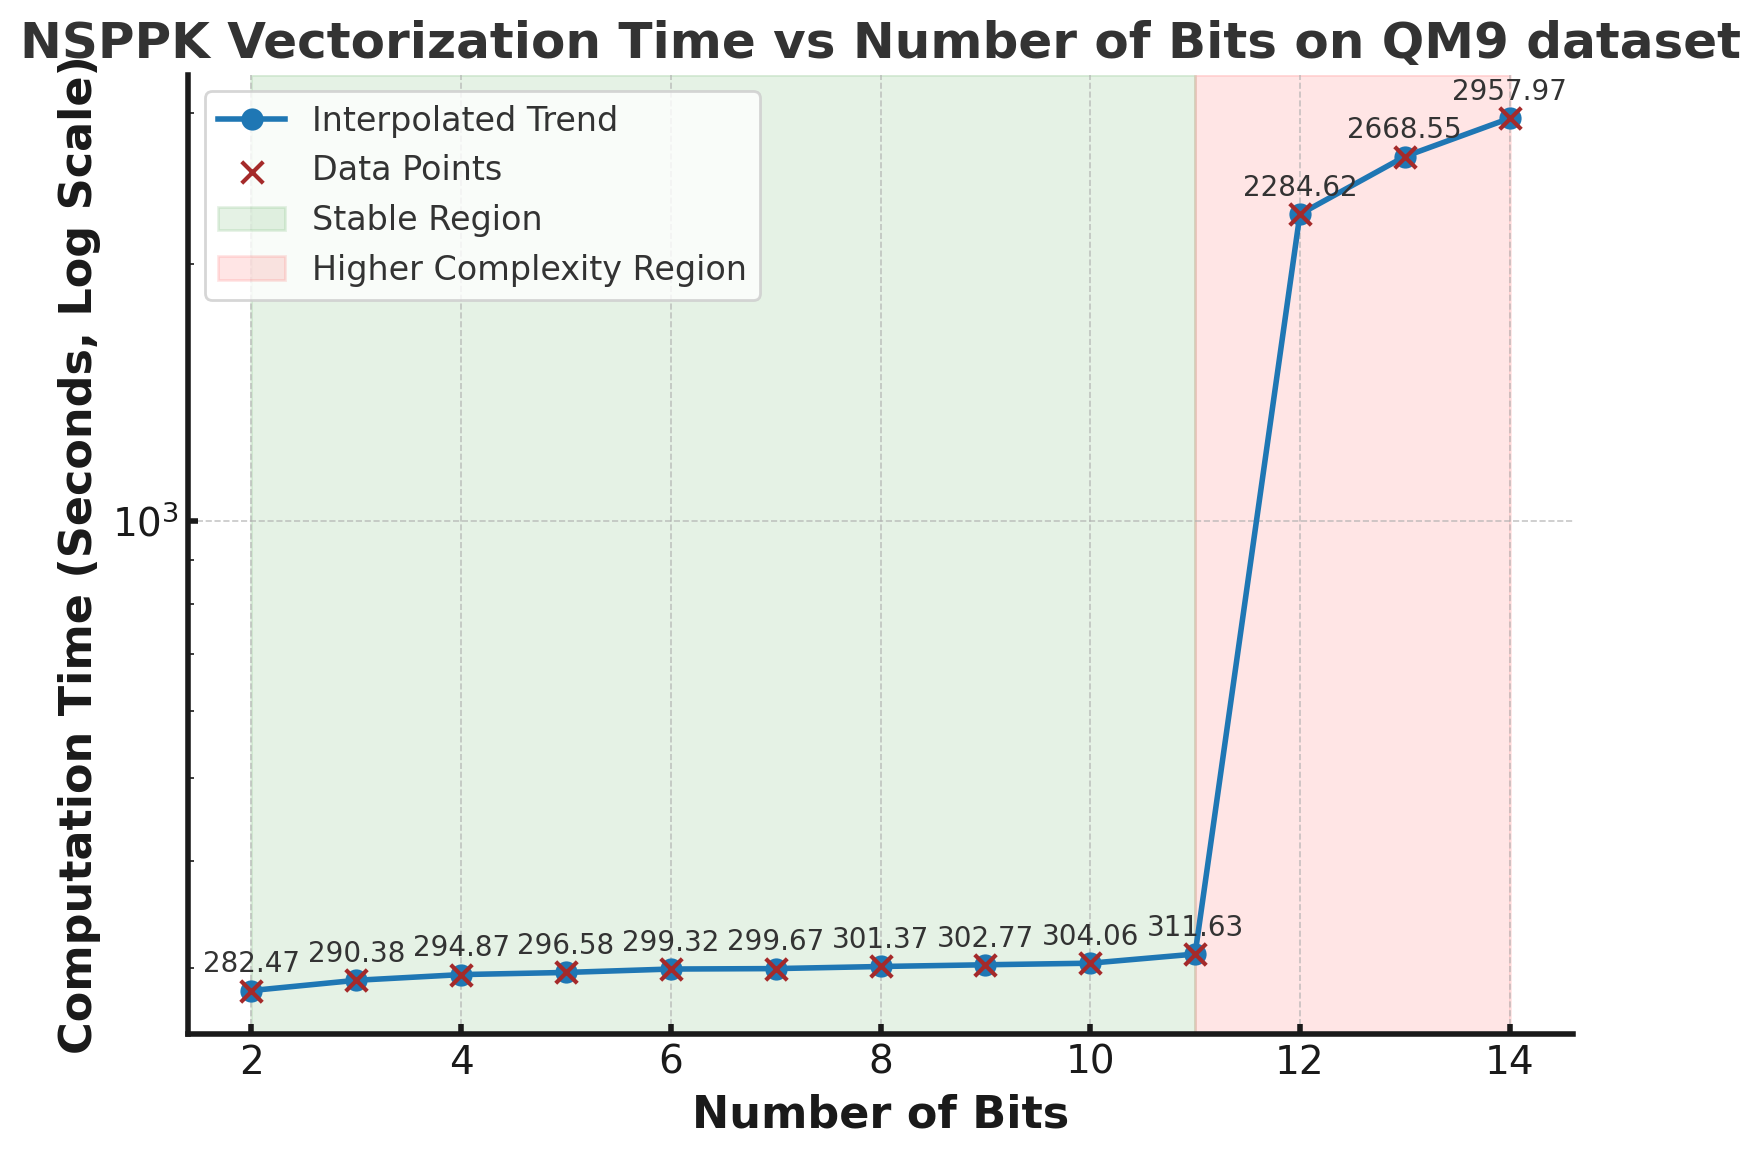
\includegraphics[width=0.8\textwidth]{images/qm9_plot.png}
    \caption{NSPPK vectorisation time for QM9 dataset as a function of number of bits.}
    \label{fig:nsppk_qm9}
\end{figure}

Figure \ref{fig:nsppk_qm9} illustrates the time required for NSPPK to vectorize the QM9 \cite{blum2009gdb13} dataset as a function of the number of hash bits $b$. As the number of bits increases, the vectorisation time rises accordingly, though the rate of increase is not uniform. Up to 11 bits, the computation time remains within a small range (under 7 minutes), demonstrating NSPPK’s efficiency in handling large-scale datasets.

However, a sharp increase in computation time occurs from 12 to 14 bits due to memory swapping, where the system resorts to using slower secondary storage instead of RAM. This significantly degrades performance, further emphasising the importance of efficient memory usage when handling high-bit representations in large-scale datasets.

At $b=15$, the vectorisation process fails due to excessive memory allocation requirements. This is a consequence of the exponential growth of the feature space: $b=15$ corresponds to a \(2^{15}\)-dimensional hash codomain, resulting in an immense memory footprint when applied to over 129,000 molecular graphs. While this represents a practical upper bound for single-machine processing, it highlights the need for optimised memory management strategies for ultra-high-dimensional embeddings.

Despite this limitation, NSPPK remains an effective and scalable approach for graph learning tasks, provided that memory usage is carefully managed when selecting the number of bits. Additionally, potential optimisations such as sparse representations, dimensionality reduction, or distributed processing could further enhance its applicability to even larger datasets.

The QM9 dataset itself consists of over 129,000 molecular graphs with 16 continuous node attributes, making it a computationally intensive benchmark. The results confirm that NSPPK successfully processes datasets of this magnitude while maintaining practical computation times, reinforcing its utility for real-world graph-based applications.


\section{Additional Experiments on Citation Networks}
\label{appendix:citation}

To further evaluate the robustness of NSPPK beyond molecular graphs,
we conducted experiments on three widely used citation network
benchmarks: \textbf{Cora}, \textbf{CiteSeer}, and \textbf{PubMed}.
These graphs exhibit higher-degree outliers, broader graph diameters,
and citation-style connectivity patterns, in contrast to the smaller
and sparser molecular graphs considered elsewhere in this work.

\begin{table}[h]
\centering
\caption{Citation network statistics and NSPPK encoding time.}
\scriptsize
\setlength{\tabcolsep}{4pt}
\begin{tabular}{lrrrrr}
\toprule
Dataset & \#Nodes & \#Edges & Avg Deg. & Max Deg. & Encoding Time (s) \\
\midrule
Cora     & 2{,}708  & 5{,}278  & 3.90 & 168 & 0.7897 \\
Citeseer & 3{,}327  & 4{,}552  & 2.74 & 99  & 0.7447 \\
PubMed   & 19{,}717 & 44{,}324 & 4.50 & 171 & 0.8747 \\
\bottomrule
\end{tabular}
\end{table}

\paragraph{Baselines.}
We compared NSPPK against a set of commonly used graph neural
network architectures for node classification:
GCN~\citep{kipf2017semi},
GAT~\citep{velivckovic2018gat},
GraphSAGE~\citep{hamilton2017graphsage},
GIN~\citep{xu2019powerful},
SGC~\citep{wu2019simplifying},
APPNP~\citep{klicpera2019predict},
and a feature-only MLP baseline.

\paragraph{Neural model configuration.}
All GNN models were trained on the original citation graphs using
the same 80/20 train--test split as NSPPK.

For GCN, GIN, GraphSAGE, and GAT we used two-layer architectures
with hidden dimension 64, ReLU activations, and dropout between
layers. GAT employed eight attention heads in the first layer.

APPNP was implemented as a two-layer MLP followed by personalized
PageRank propagation with $K=10$ steps and teleport probability
$\alpha=0.1$. SGC used a single linear classifier with $K=2$
propagation steps.

All models were trained using the Adam optimizer
(learning rate 0.01, weight decay $5\times10^{-4}$) for 200 epochs.
Model selection relied solely on the fixed training split,
without dataset-specific hyperparameter tuning.
Performance is reported using macro-averaged ROC--AUC.

\paragraph{NSPPK configuration.}
For the citation-network experiments, we retained the same general NSPPK
construction but used $R=1$, $D=4$, $R'=0$, and 11-bit hashing.

Continuous node attributes were projected to 24 dimensions using SVD.
Because NSPPK requires discrete node labels, we applied $k$-means
clustering with $k=5$ on the node attribute vectors and assigned
cluster memberships as node labels.


\section{Large-Scale Experiment: MolPCBA Learning Curves and Efficiency}
\label{appendix:molpcba}

We evaluated NSPPK on the large-scale \texttt{ogbg-molpcba} benchmark from the Open Graph Benchmark suite \cite{hu2020ogb}, which includes  437,929 node attributed molecular graphs and 128 binary classification tasks.  
In practice, many of these tasks are both sparse (due to missing labels) and highly imbalanced.





\section{Case Study: Target 95 from \texttt{ogbg-molpcba}}
We further examined \textbf{task~95}, which provides 48,853 positive examples, 293,968 negatives, and 95,108 molecules with missing labels. 
To analyze sample efficiency, we subsampled balanced datasets up to \textbf{78,164 labelled graphs} (positives and negatives in equal proportion) and varied the training set size from 100 to 250k examples.  
Each experiment was repeated with \textbf{five random seeds}, and average precision (AP) was reported.  
In parallel, we also trained each baseline once on the \emph{full OGB scaffold split} (249,715 train, 29,826 validation, 29,427 test).  

We compared NSPPK in combination with different downstream classifiers—logistic regression, random forest, and XGBoost—using both \emph{sparse} and \emph{dense} feature representations, against neural baselines including GIN, GAT, PNA, PDF, a generic GNN, and AttentiveFP (FNP).  
The distinction between sparse and dense refers only to feature storage: sparse matrices retain only nonzeros and are CPU-efficient, while dense mode expands full vectors (more memory, but occasionally favourable for GPU kernels).

For NSPPK, we fixed a single configuration (\(R=1\), \(D=4\), \(R'=1\), \(n_{\text{bits}}=16\)) across all runs.  (see Appendix~\ref{appendix:task95} for full implementation details of the graph neural networks models used within this experiment).


Figure~\ref{fig:appendix_large_experiment} summarizes the results.  
NSPPK shows strong sample efficiency, achieving higher AP than all neural baselines at small training sizes.  
Its runtime is also favourable: sparse variants in particular remain substantially faster to train than graph neural networks.  
At scale, PDF overtakes NSPPK in predictive performance, though the gap remains small.  
Interestingly, NSPPK combined with logistic regression can take as long as a GNN to train, but still delivers superior AP on small data regimes.  
Overall, NSPPK offers a simple, lightweight alternative that competes directly with neural methods.
Figure~\ref{fig:appendix_large_experiment} shows the resulting learning curves, with all NSPPK variants highlighted in red.  
\begin{figure}[H]
  \centering
  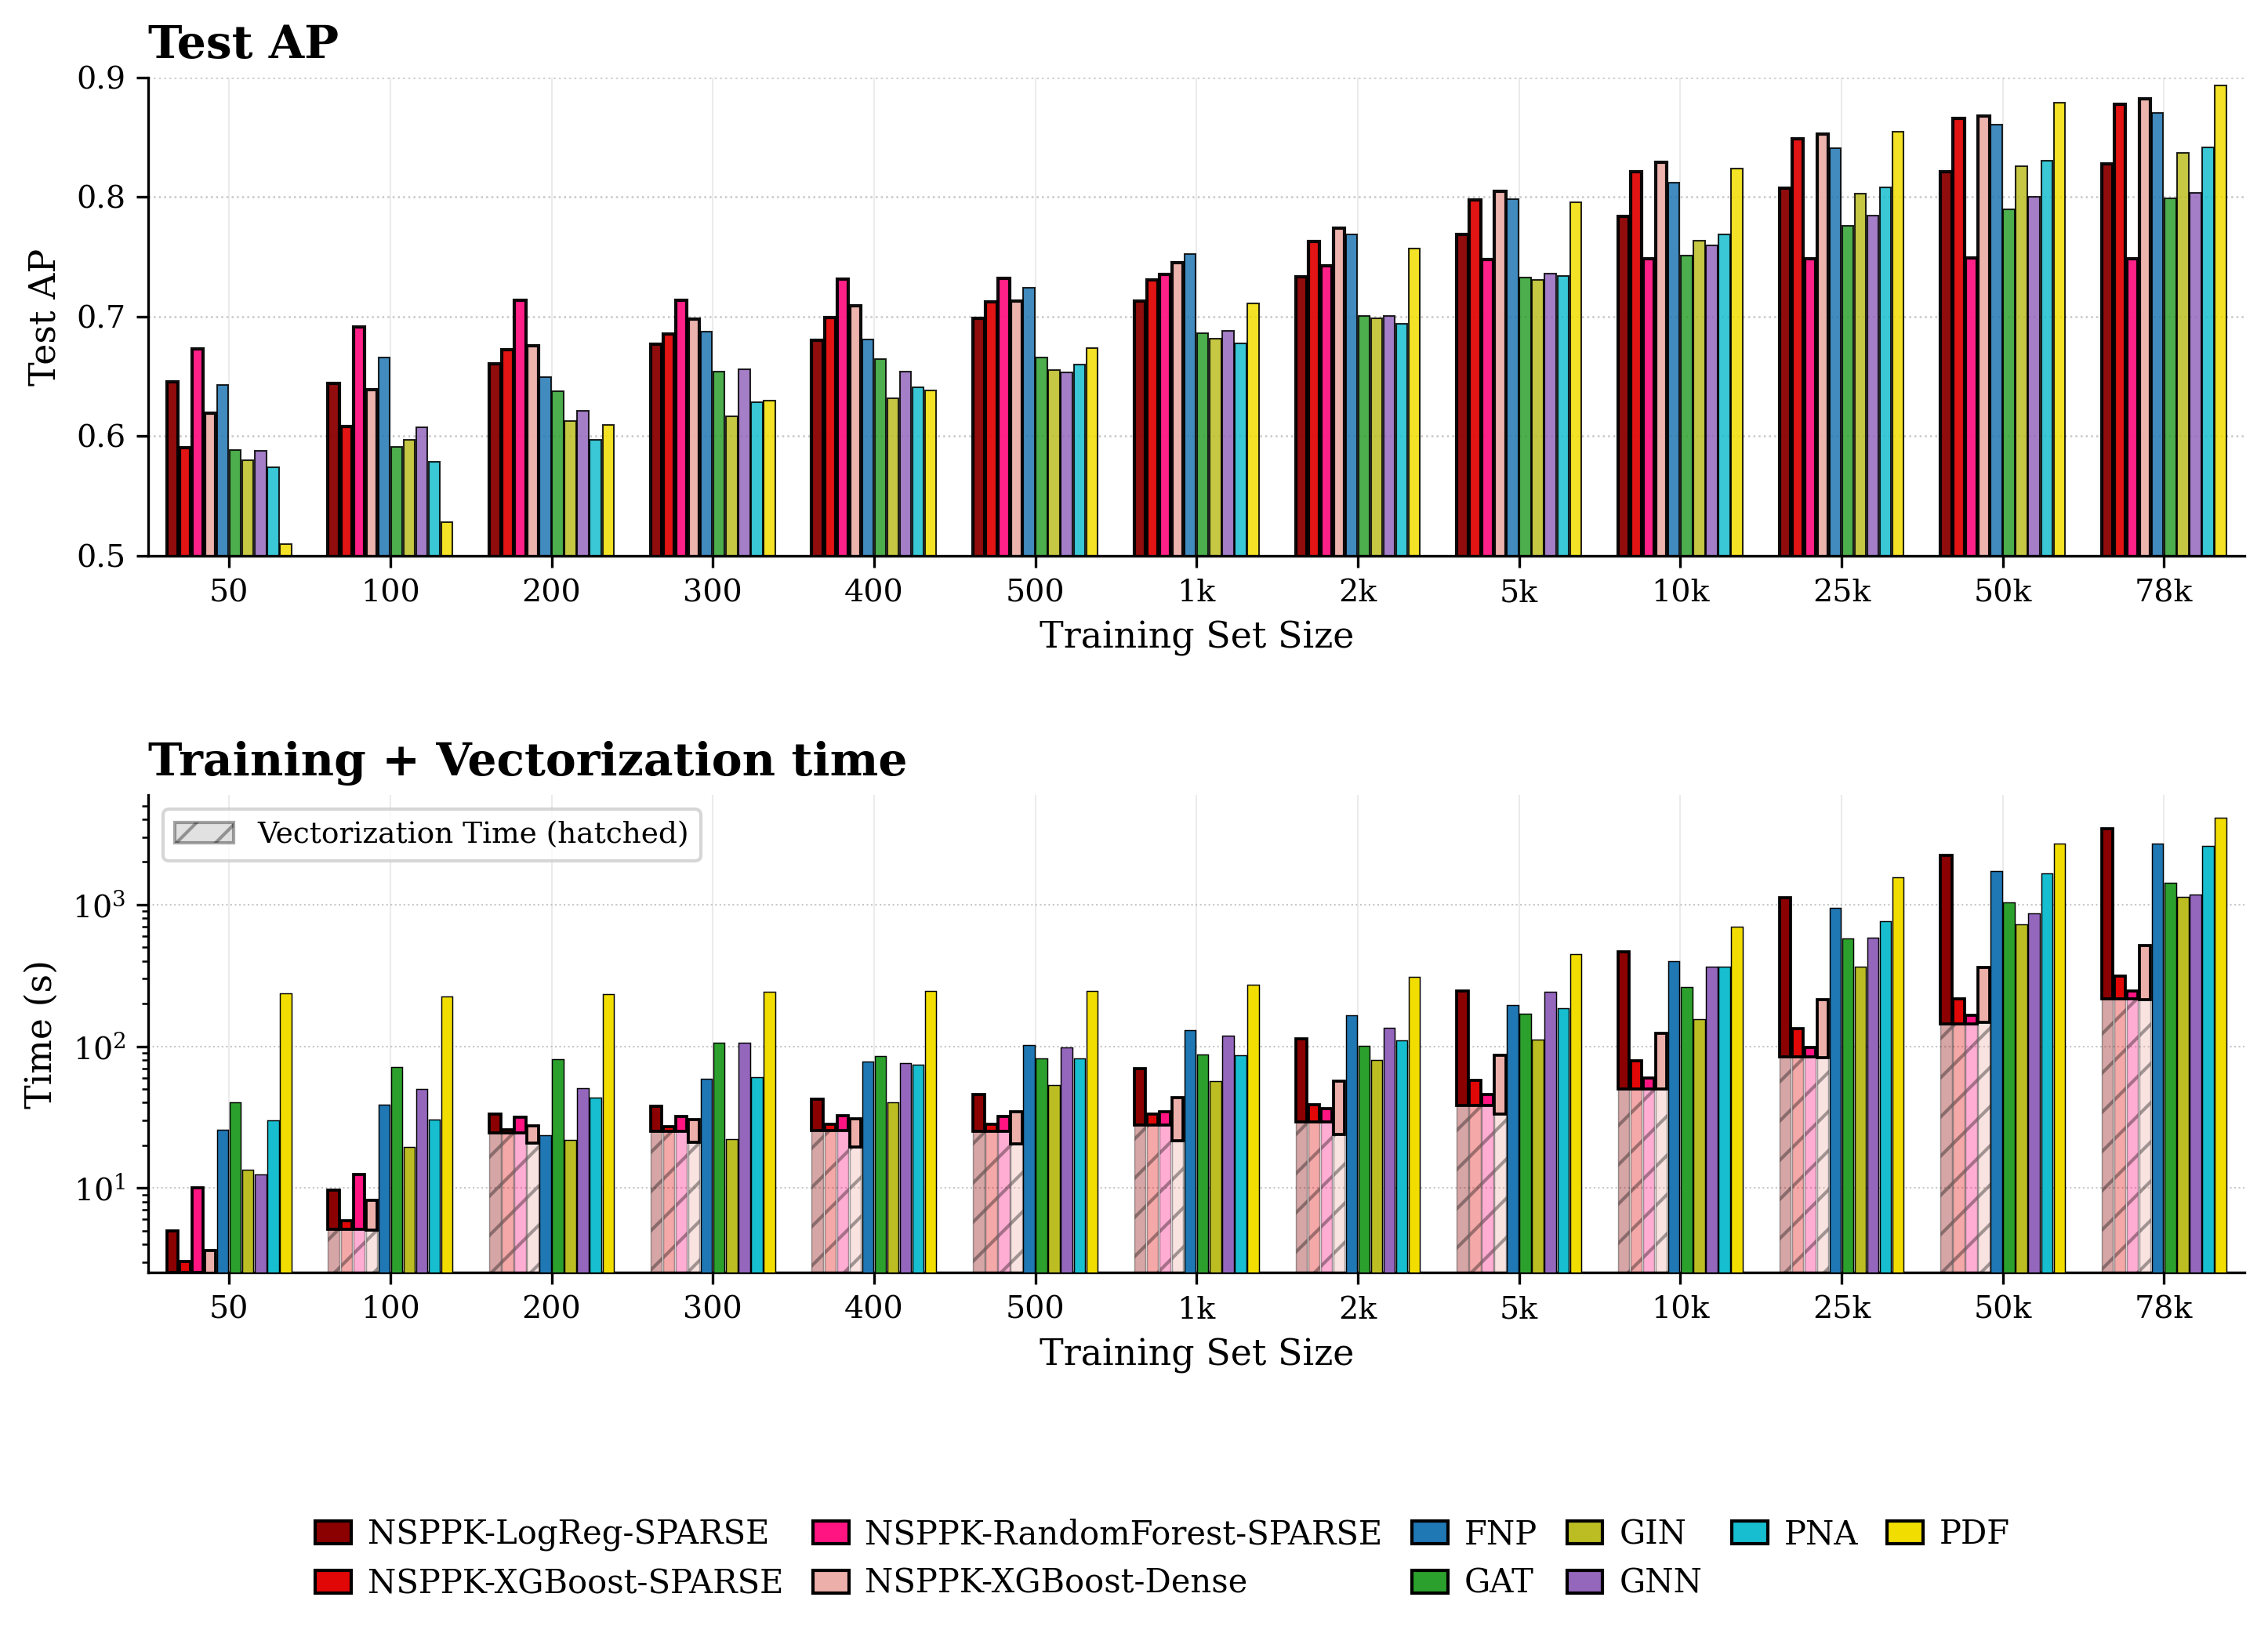
\includegraphics[width=1\textwidth]{images/large_experiment.png}
  \caption{Learning curves on \texttt{ogbg-molpcba} (task 95). NSPPK (red) paired with different downstream classifiers is compared against neural baselines including GIN, GAT, PNA, PDF, and AttentiveFP (FNP).}
  \label{fig:appendix_large_experiment}
\end{figure}

\section{Implementation Details for Task~95 Experiments}
\label{appendix:task95}

\paragraph{NSPPK Configuration.}
For all NSPPK experiments we fixed the parameters across classifiers:
\[
R=1, \quad D=4, \quad R'=1, \quad n_{\text{bits}}=16 .
\]

Both sparse and dense feature representations were evaluated.
Sparse mode stores only non-zero entries and is efficient for CPU-based
models, while dense mode expands the full feature vectors, which can
occasionally benefit GPU-accelerated tree methods.

\paragraph{Downstream Classifiers.}
The exact settings for the classifiers paired with NSPPK features are given in
Table~\ref{tab:nsppk-classifiers}.

\begin{table}[H]
\centering
\caption{Classifiers used with NSPPK features on \texttt{ogbg-molpcba} (task 95).}
\label{tab:nsppk-classifiers}
\begin{tabular}{l l p{7cm}}
\toprule
Classifier & Features & Configuration \\
\midrule
Logistic Regression & Sparse & \texttt{saga}, max\_iter=1000, $L_2$, $n_{\text{jobs}}=64$ \\
Random Forest & Sparse & 500 trees, depth=5, $n_{\text{jobs}}=64$, seed=42 \\
XGBoost & Dense & 1000 trees, depth=6, LR=0.03, subsample=0.8, colsample=0.8 \\
XGBoost & Sparse & Same as above, \texttt{hist} backend \\
\bottomrule
\end{tabular}
\end{table}

\paragraph{Neural Baselines.}
For comparison, we trained common GNN baselines using published
hyperparameters. Table~\ref{tab:nn-baselines} summarizes the main
configurations.

\begin{table}[H]
\centering
\caption{Neural baselines and their configurations for task 95.}
\label{tab:nn-baselines}
\begin{tabular}{l p{7cm} l}
\toprule
Model & Main hyperparameters & Source \\
\midrule
PNA & 2 layers, dim $64\rightarrow32$, batch 64/256, LR=0.001, Adam & \cite{corso2020pna} \\
PDF (Basis-DGL) & 8 layers, dim 384, batch 64/256, LR=$5\times10^{-4}$, AdamW & \cite{yang2023pdf} \\
GAT & 2 layers, dim $64\rightarrow32$, 4/1 heads, LR=0.001, Adam & \cite{velivckovic2018gat} \\
AttentiveFP (FNP) & 4 layers, dim 64, dropout=0.2, LR=0.001, Adam & \cite{xiong2019attentivefp} \\
GIN & 2 layers, dim $64\rightarrow32$, LR=0.001, Adam & \cite{xu2019powerful} \\
GCN (OGB baseline) & 2 layers, dim $64\rightarrow32$, LR=0.001, Adam & \cite{hu2020ogb} \\
\bottomrule
\end{tabular}
\end{table}

\paragraph{Shared Training Setup.}
All neural baselines were trained on the official OGB scaffold split
(train: 249,715; validation: 29,826; test: 29,427).
The loss function was binary cross-entropy with logits
(\texttt{BCEWithLogitsLoss}), and evaluation metrics included AP and ROC--AUC.
Unless otherwise stated, all experiments were executed on CPU.

\paragraph{Reproducibility.}
Balanced-data experiments were repeated with five random seeds.
Both feature extraction time and training time are reported in the main text.

\section{Further Visualization: Accuracy--Time Trade-off}
\label{appendix:tradeoff}

\begin{figure}[H]
\centering
\captionsetup{font=small,aboveskip=3pt,belowskip=0pt}
\captionsetup[subfigure]{font=small}

% ---------- row 1 ----------
\begin{subfigure}[t]{0.32\textwidth}
  \centering
  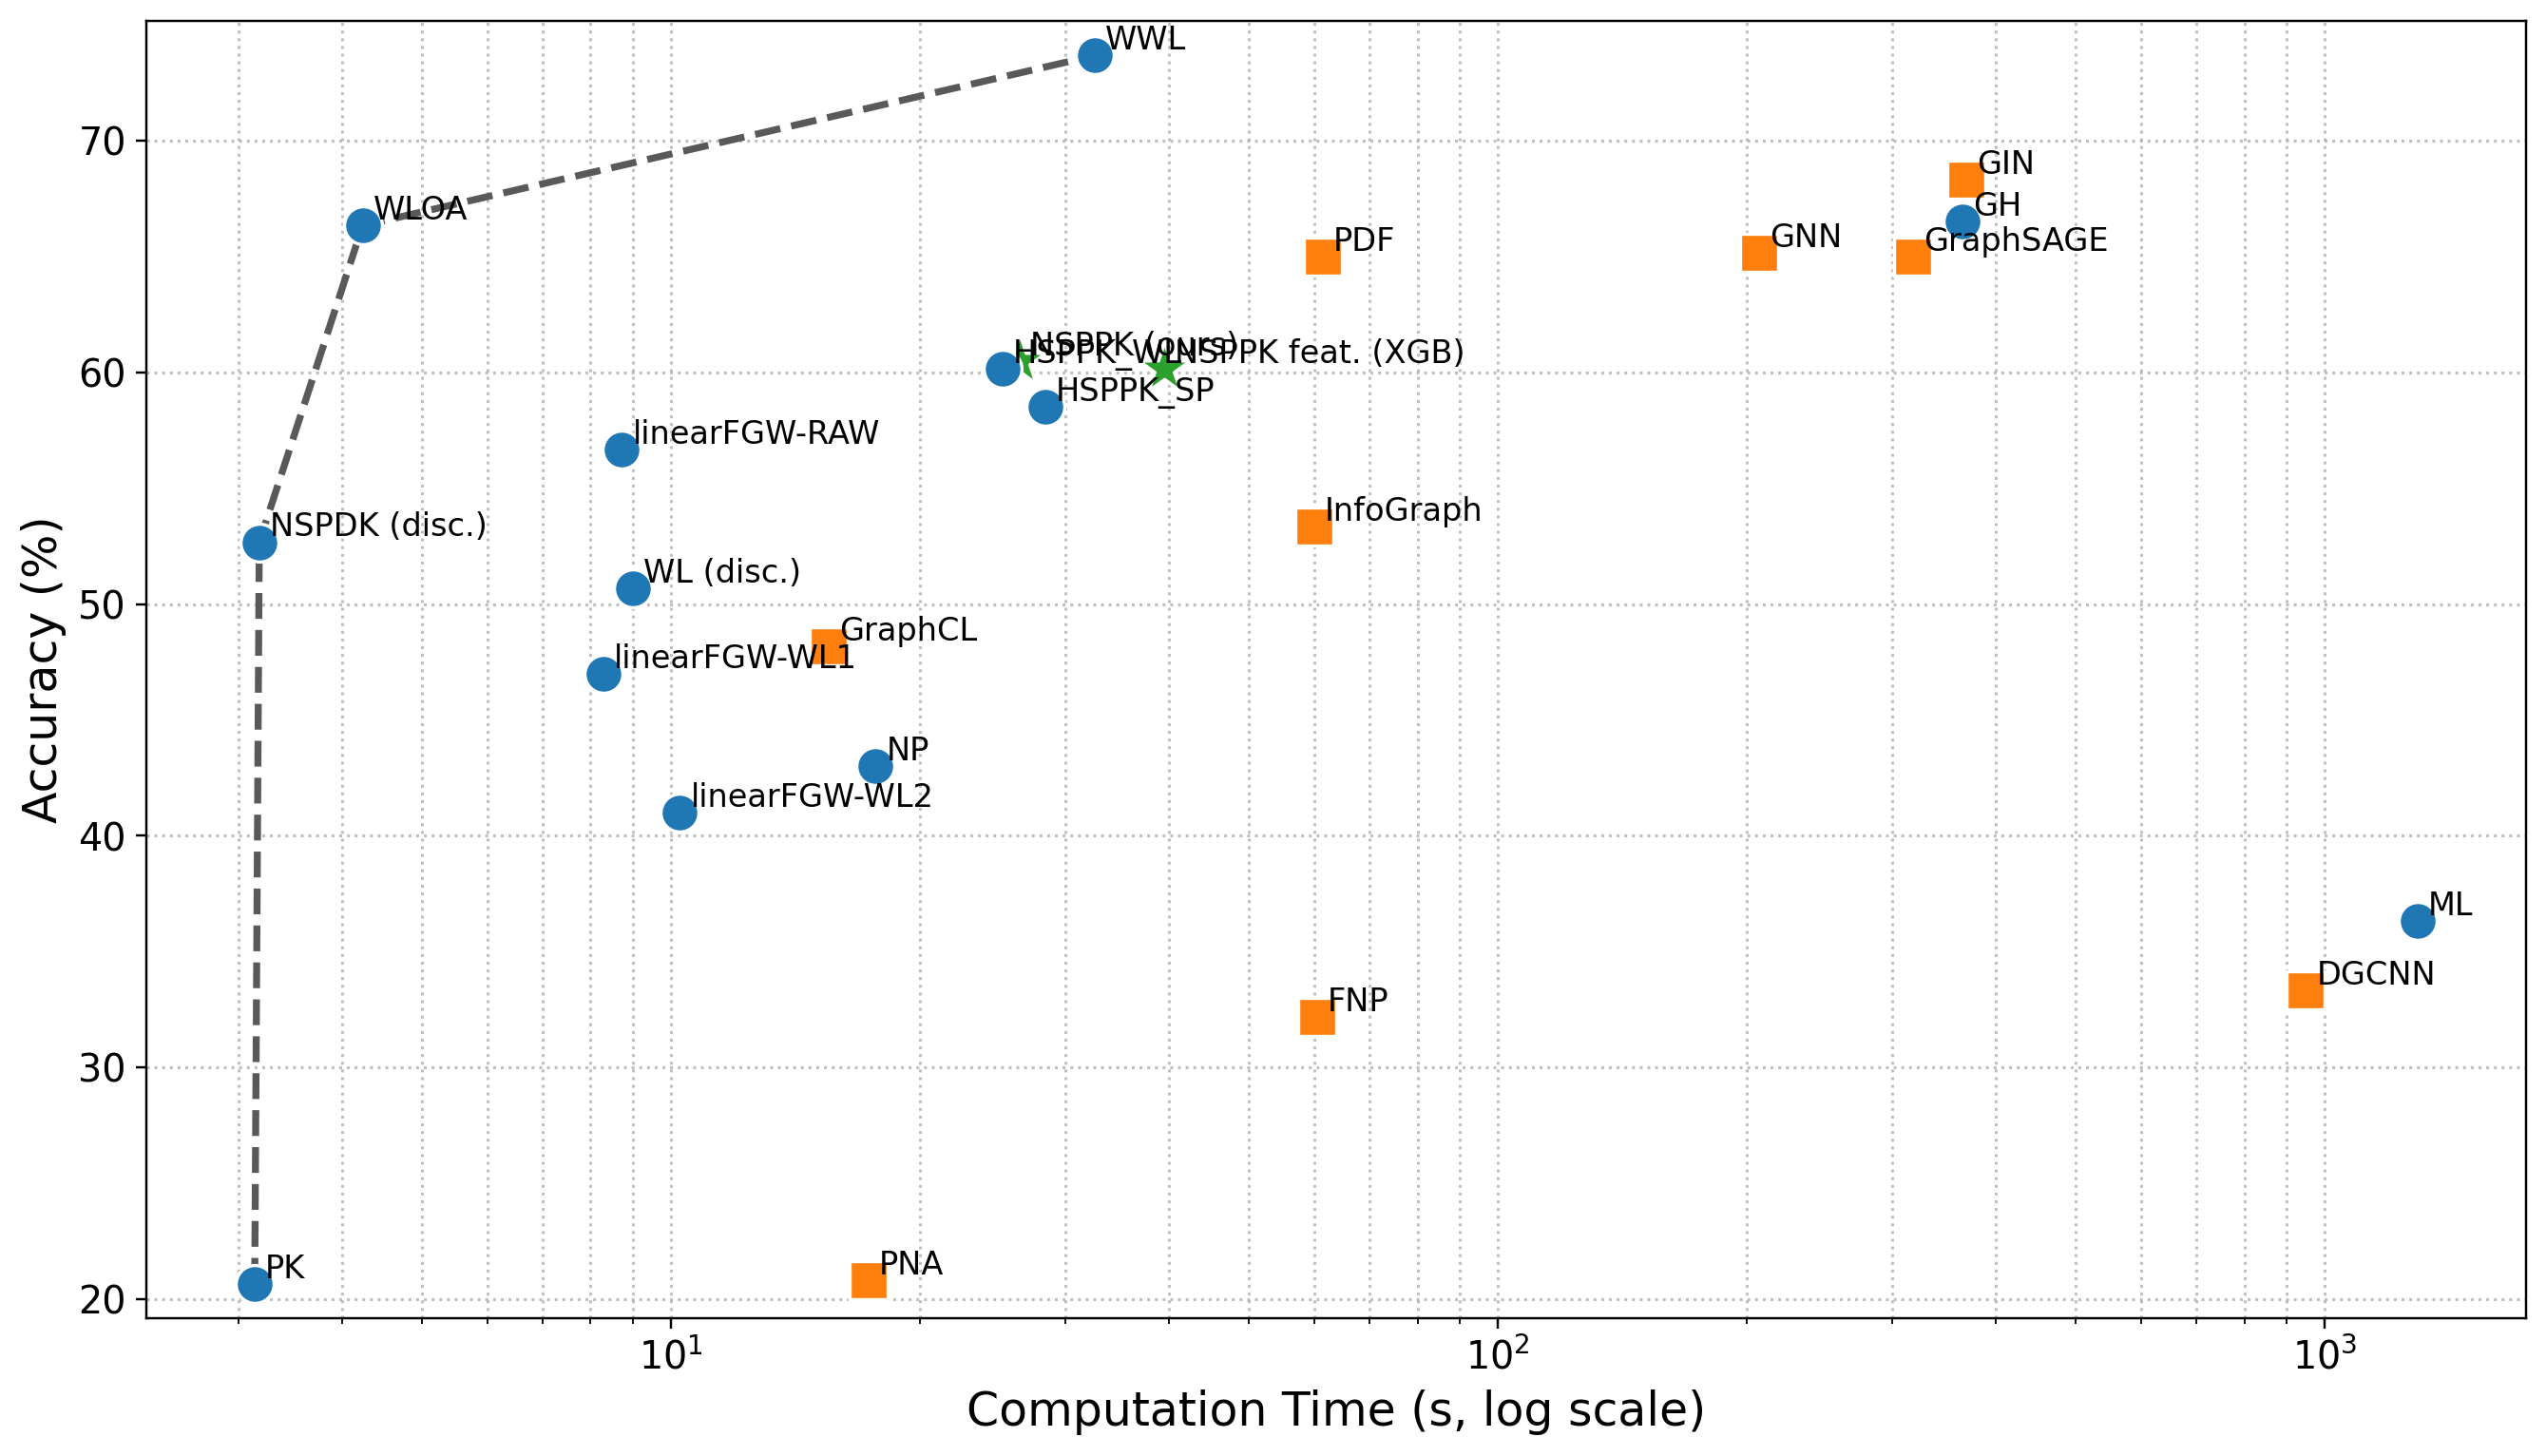
\includegraphics[width=\linewidth]{images/tradeoff_enzymes.png}
  \caption{ENZYMES}
\end{subfigure}\hfill
\begin{subfigure}[t]{0.32\textwidth}
  \centering
  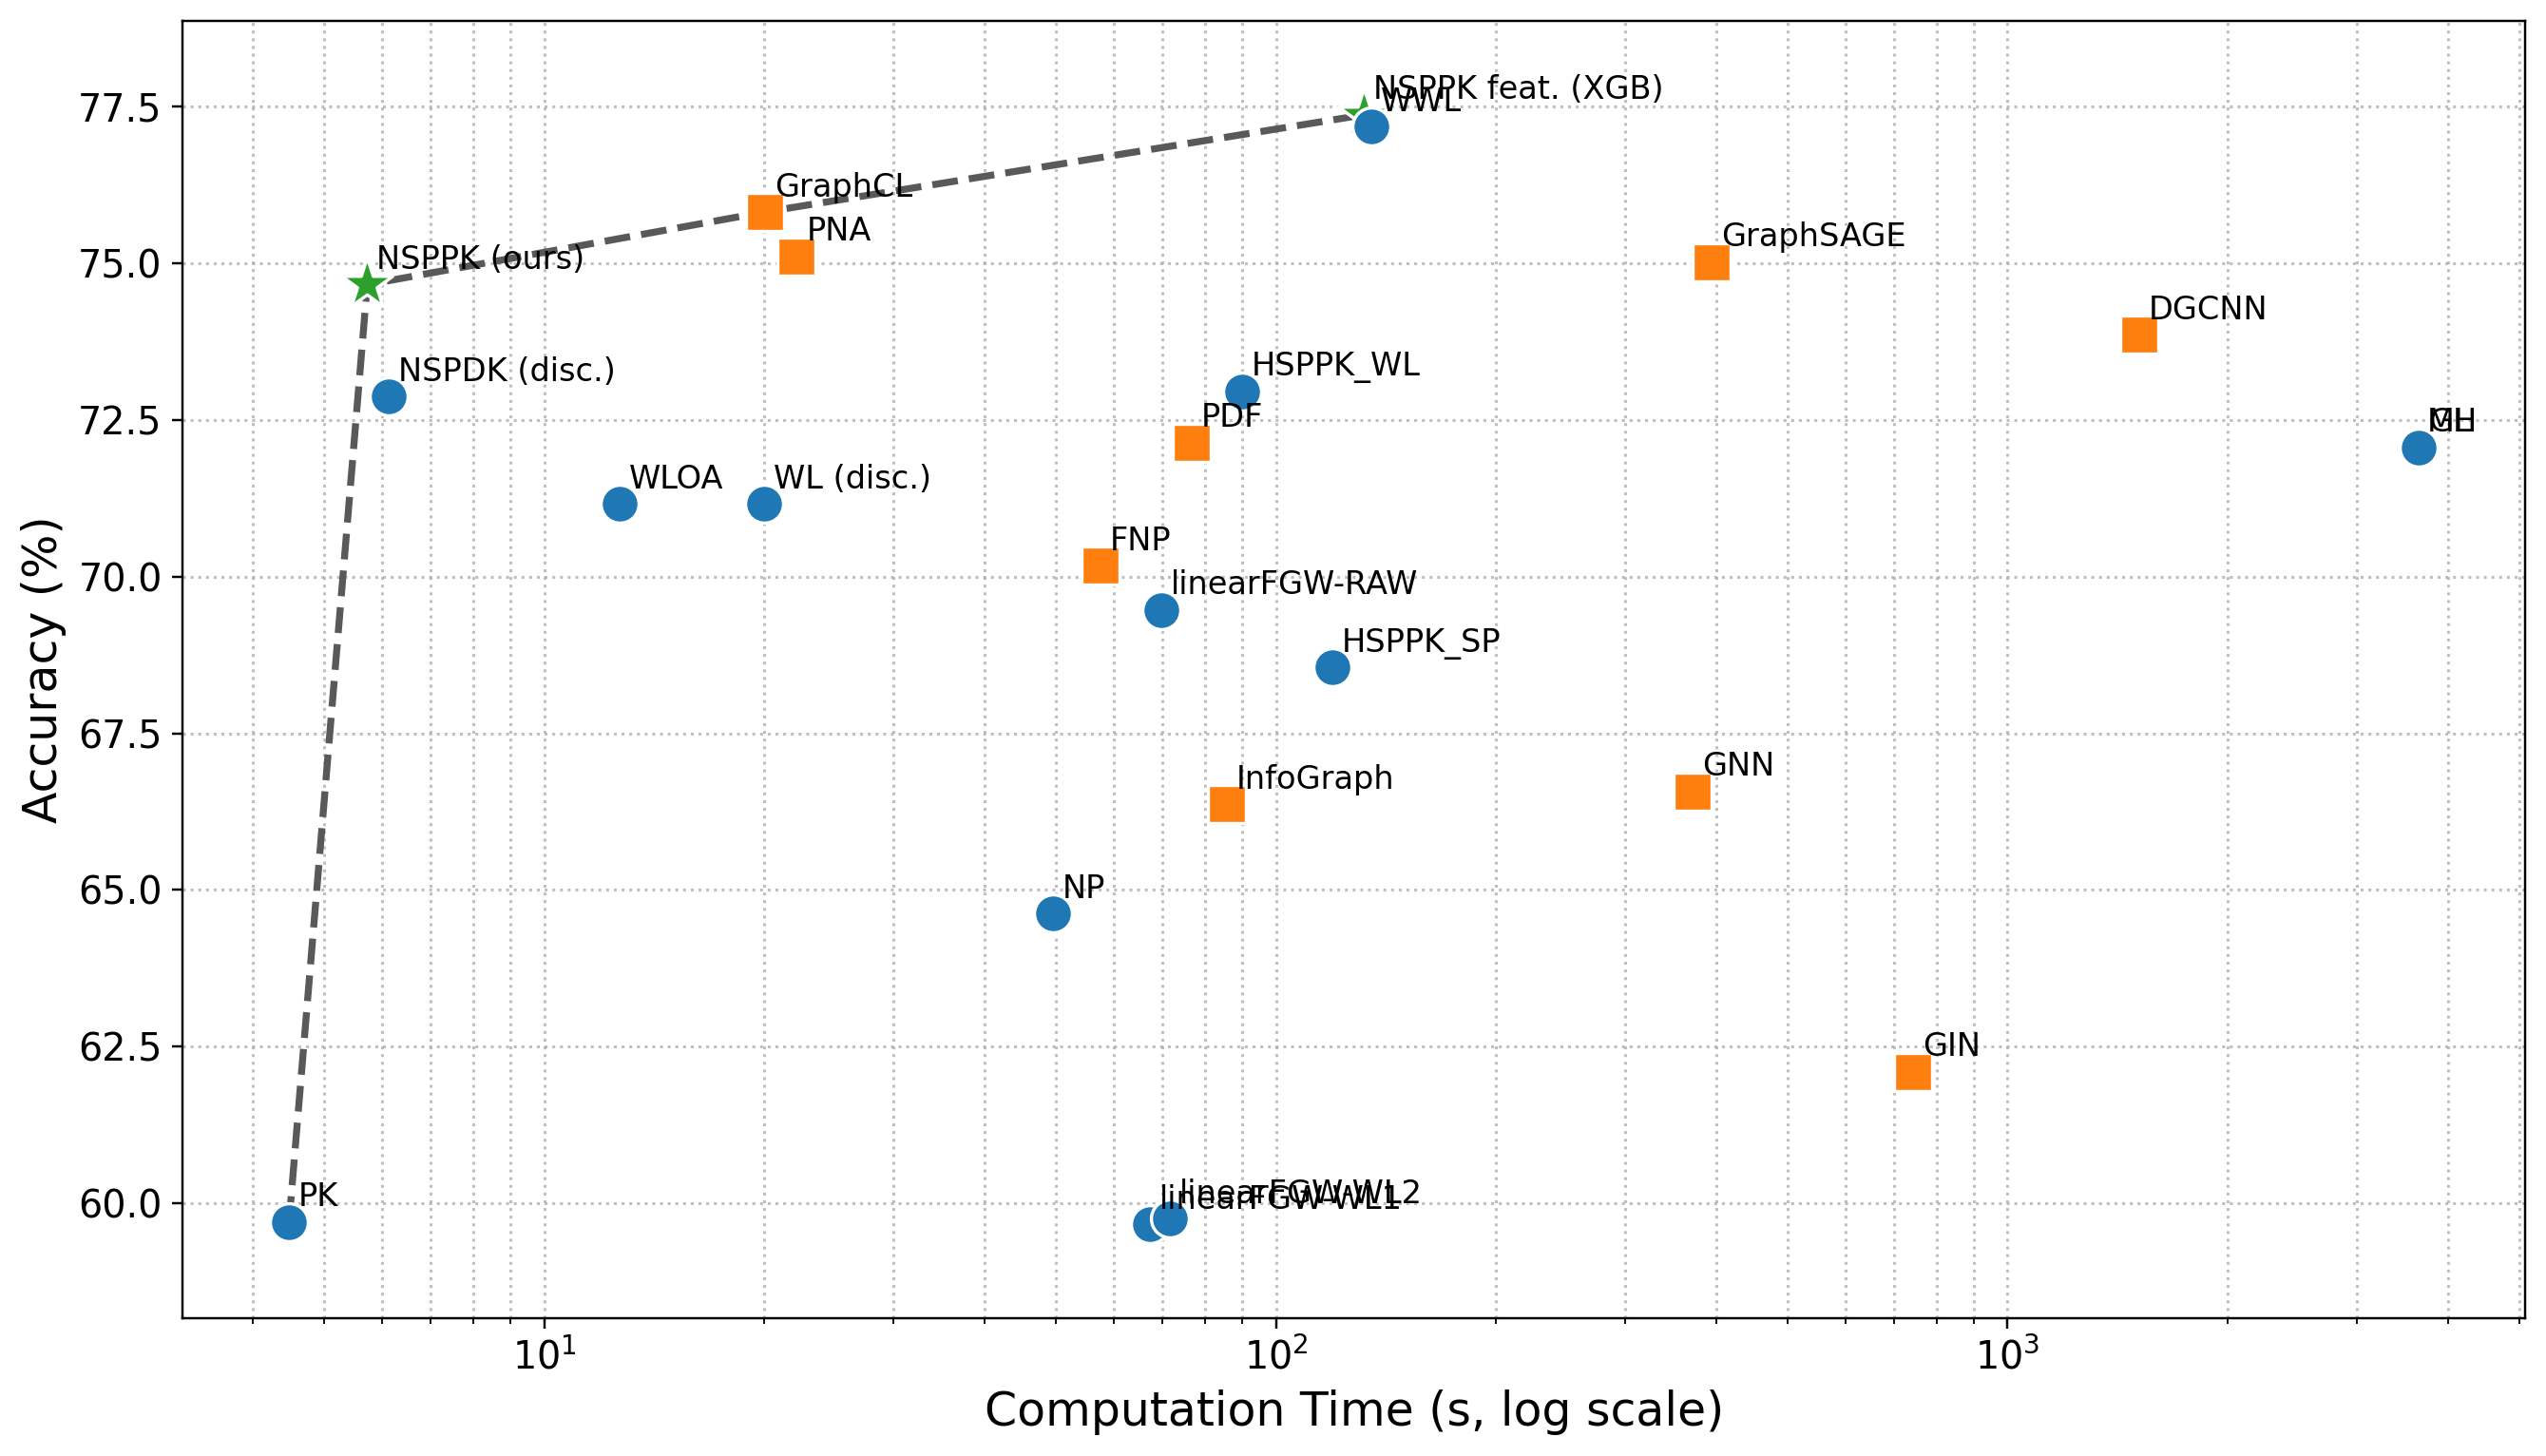
\includegraphics[width=\linewidth]{images/tradeoff_proteins.png}
  \caption{PROTEINS}
\end{subfigure}\hfill
\begin{subfigure}[t]{0.32\textwidth}
  \centering
  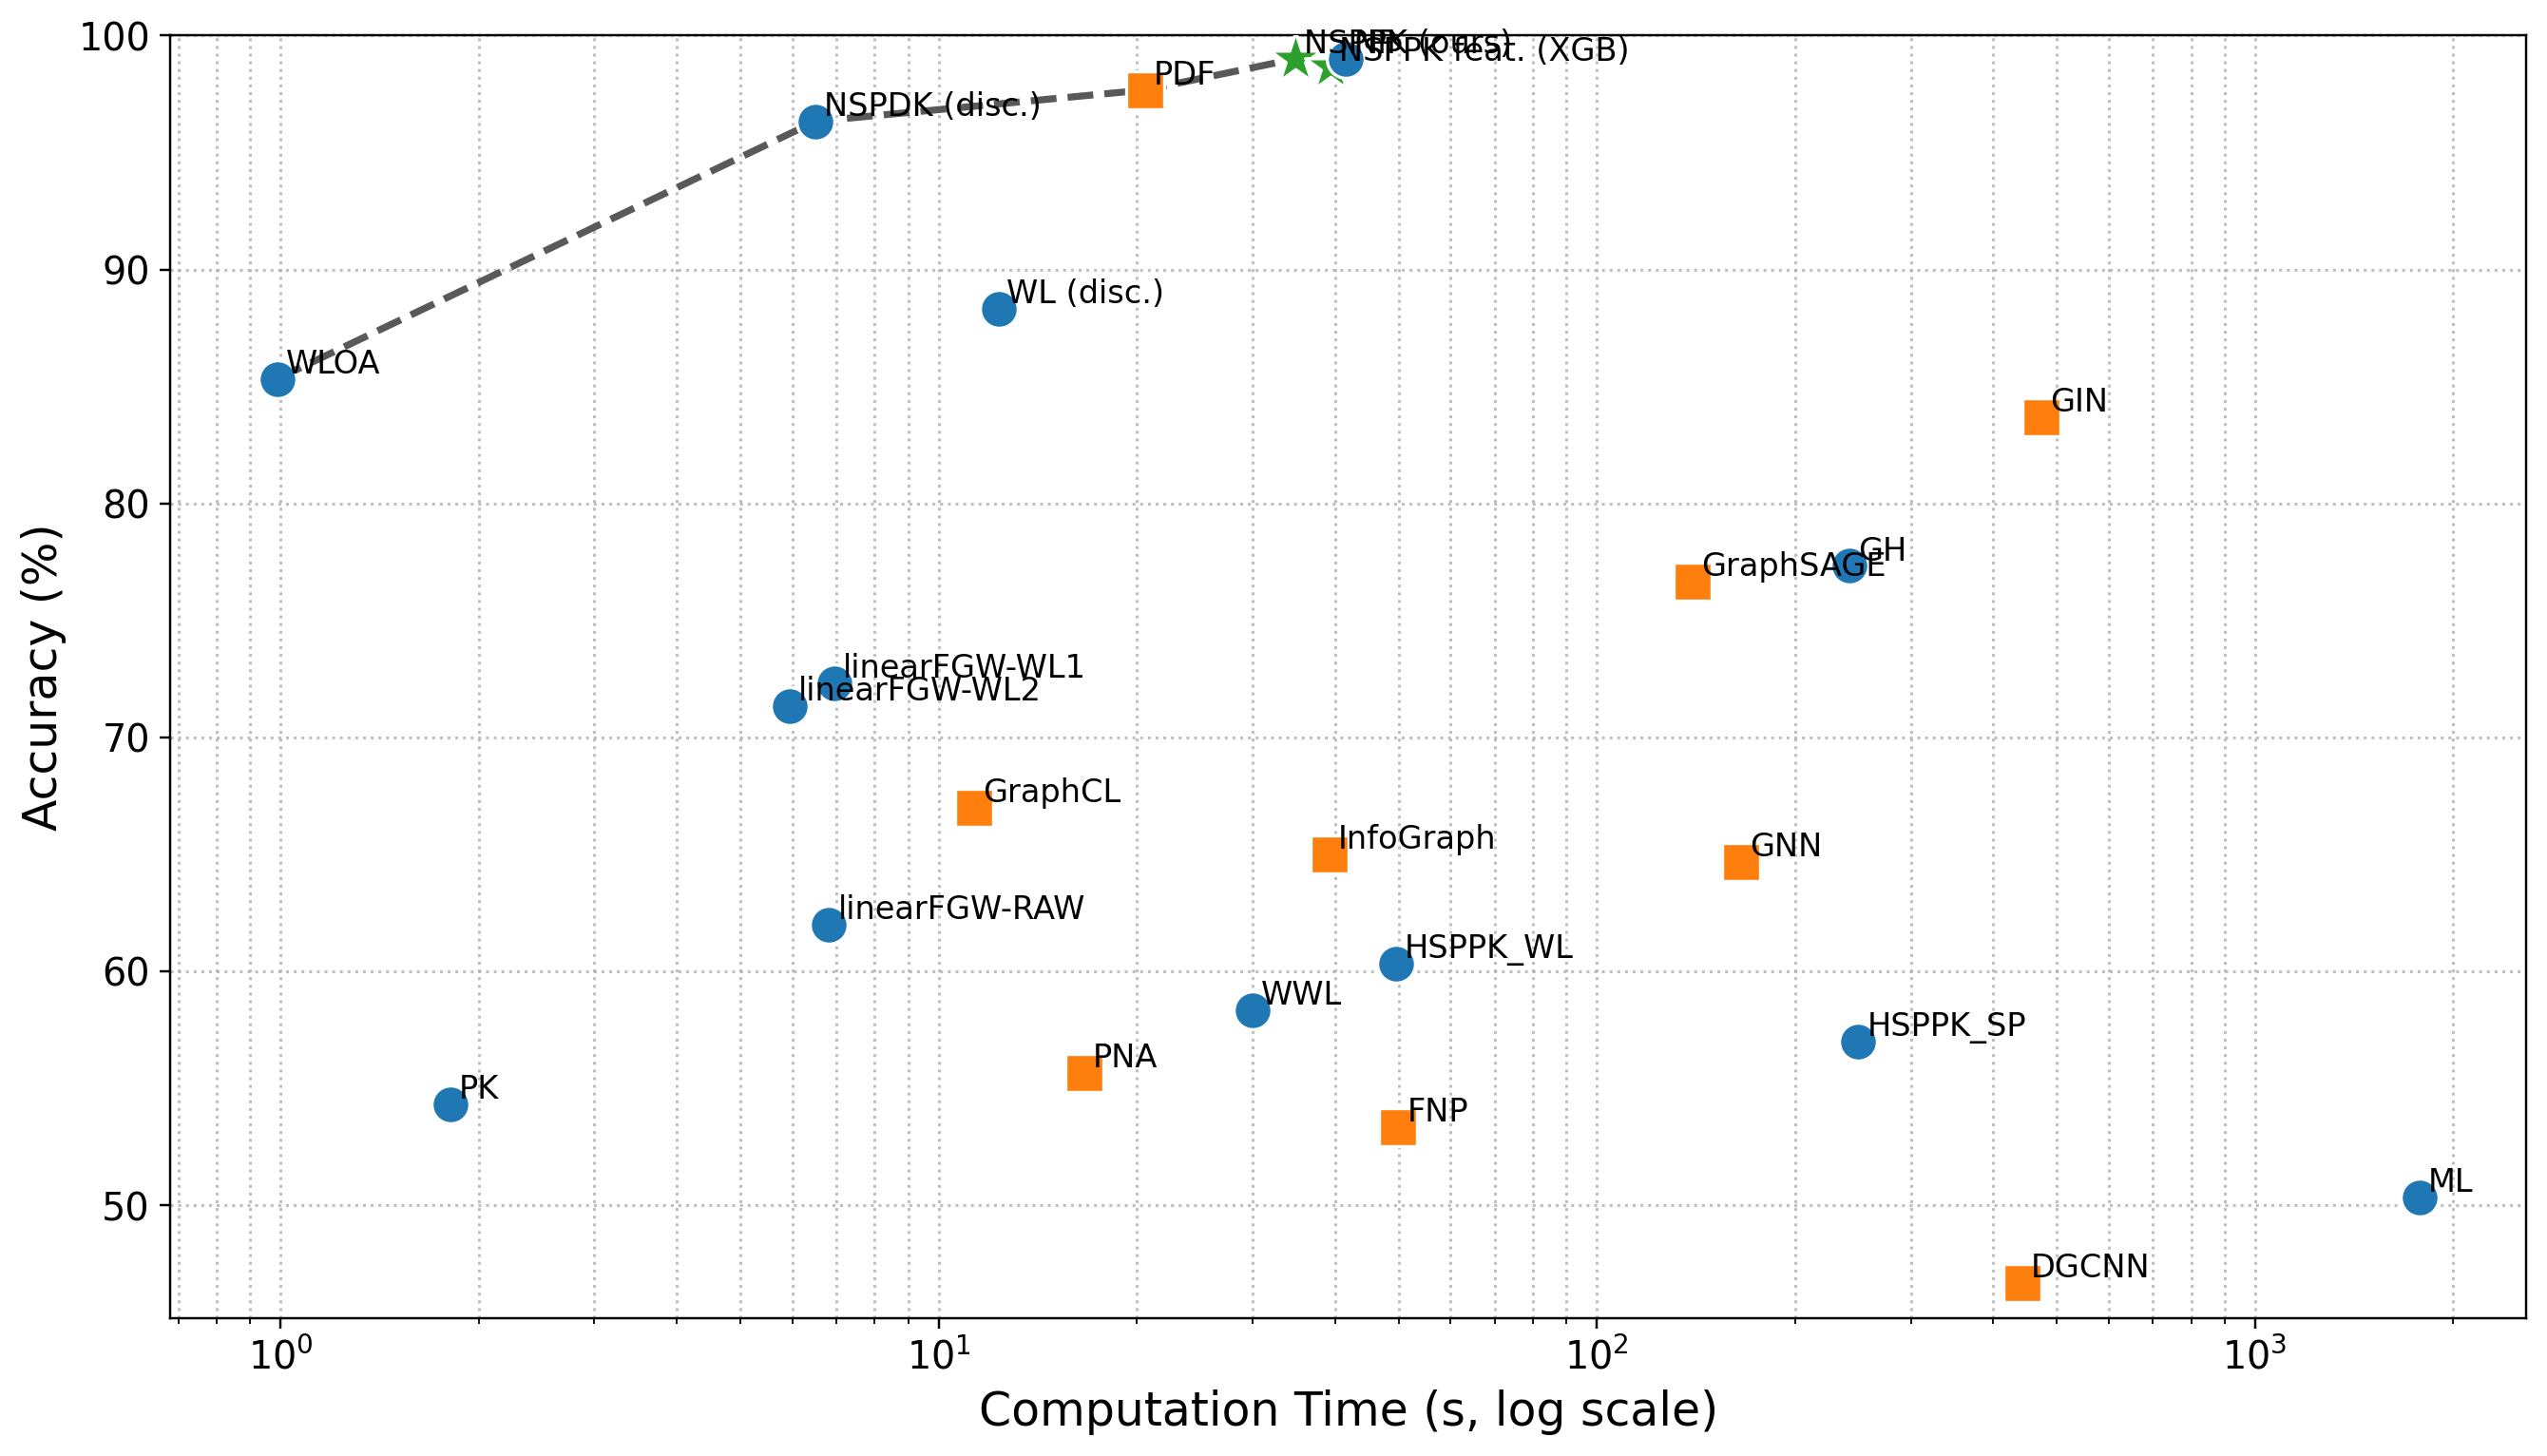
\includegraphics[width=\linewidth]{images/tradeoff_syntheticnew.png}
  \caption{SYNTHETICnew}
\end{subfigure}

\vspace{2pt}

% ---------- row 2 ----------
\begin{subfigure}[t]{0.32\textwidth}
  \centering
  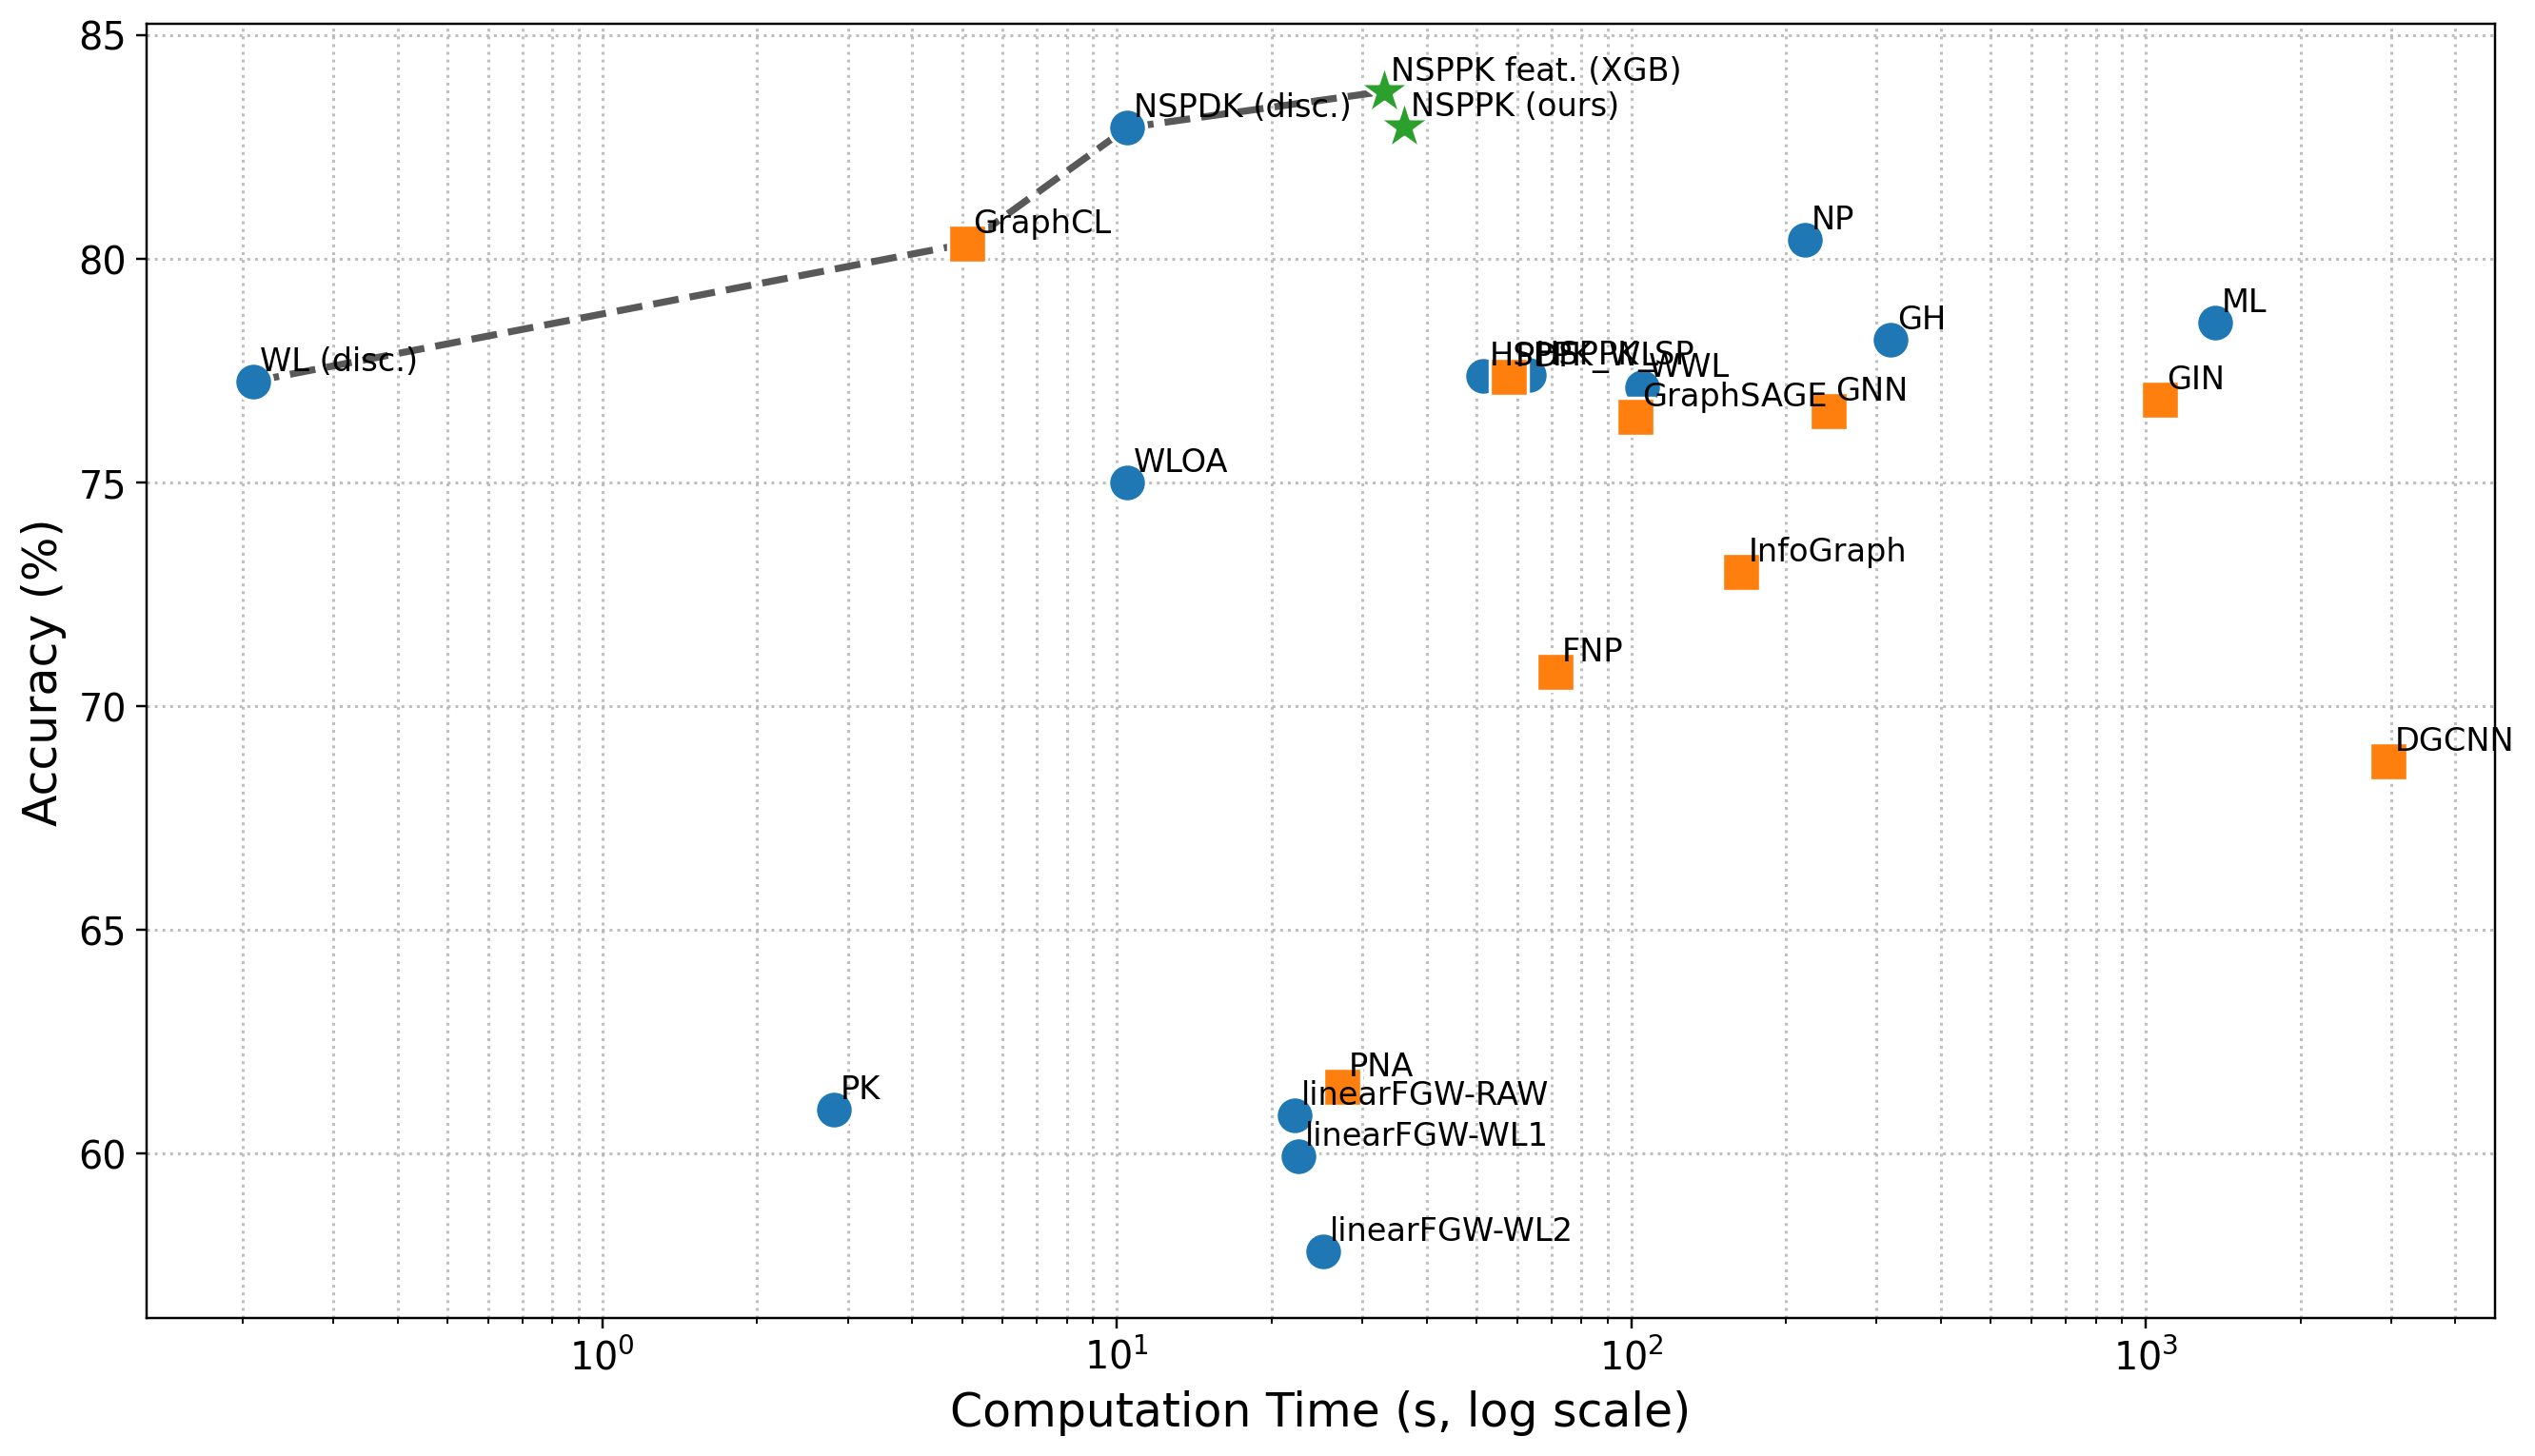
\includegraphics[width=\linewidth]{images/tradeoff_dhfr.png}
  \caption{DHFR}
\end{subfigure}\hfill
\begin{subfigure}[t]{0.32\textwidth}
  \centering
  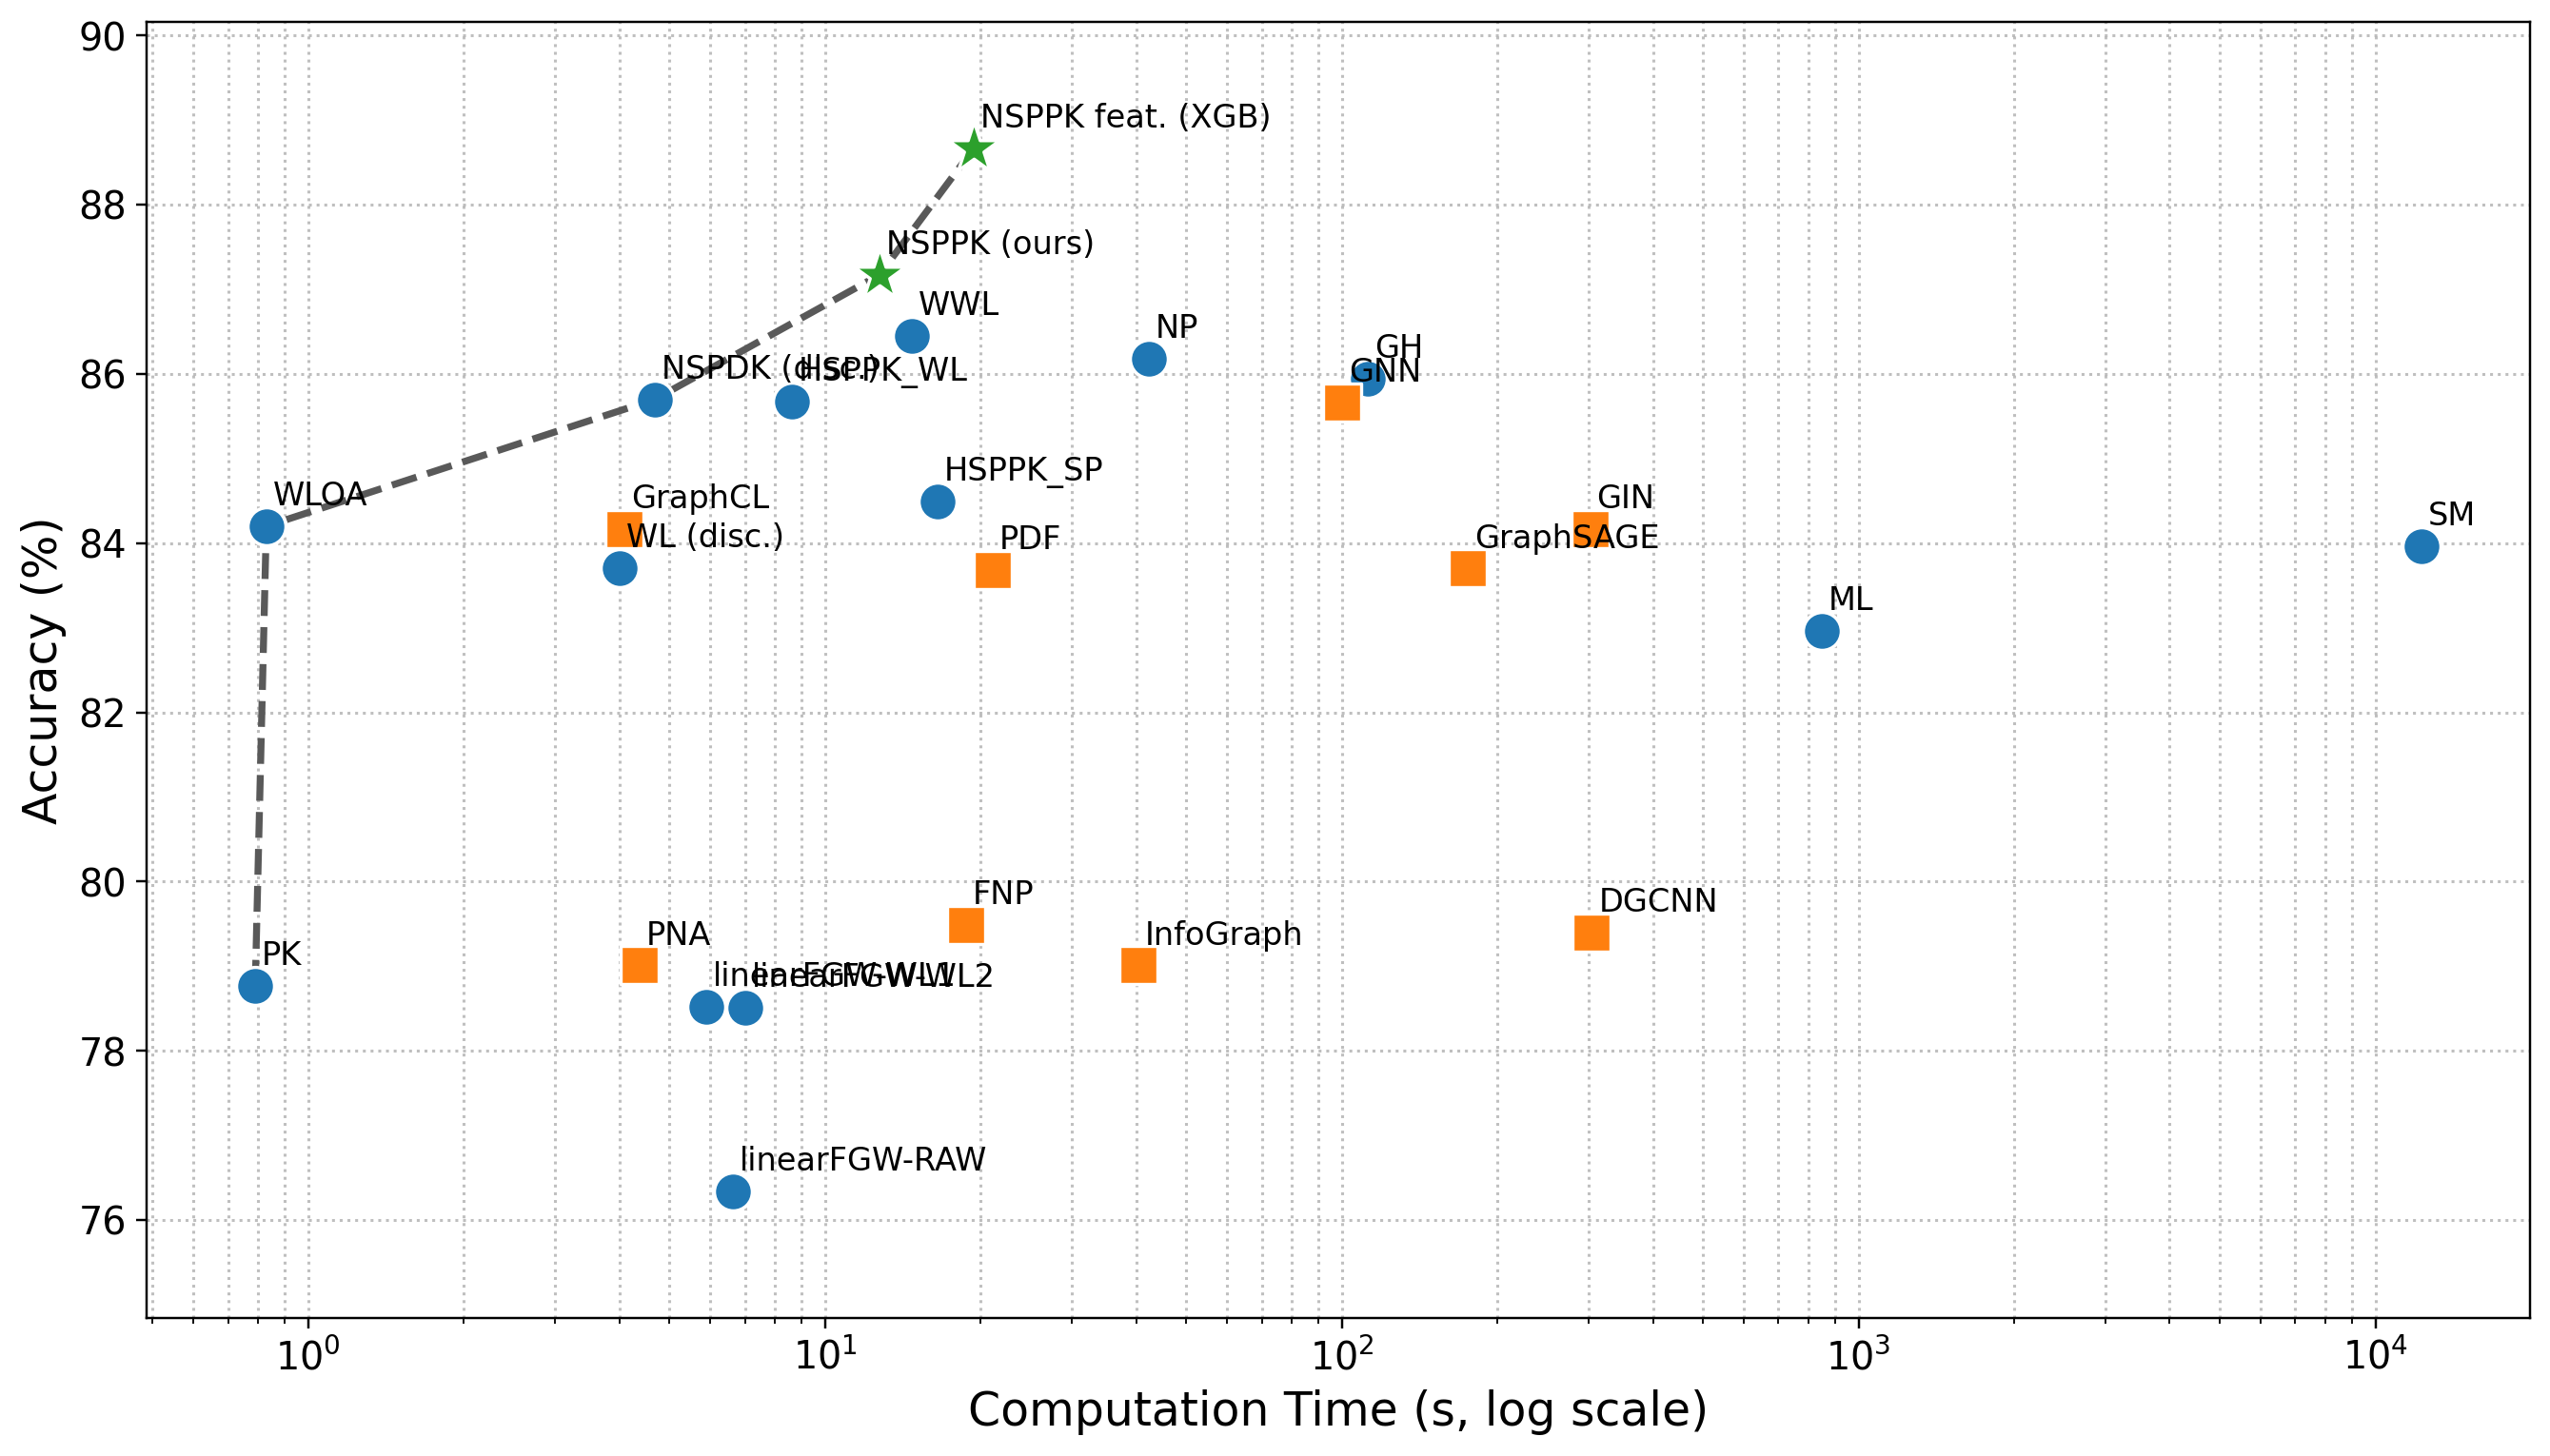
\includegraphics[width=\linewidth]{images/tradeoff_bzr.png}
  \caption{BZR}
\end{subfigure}\hfill
\begin{subfigure}[t]{0.32\textwidth}
  \centering
  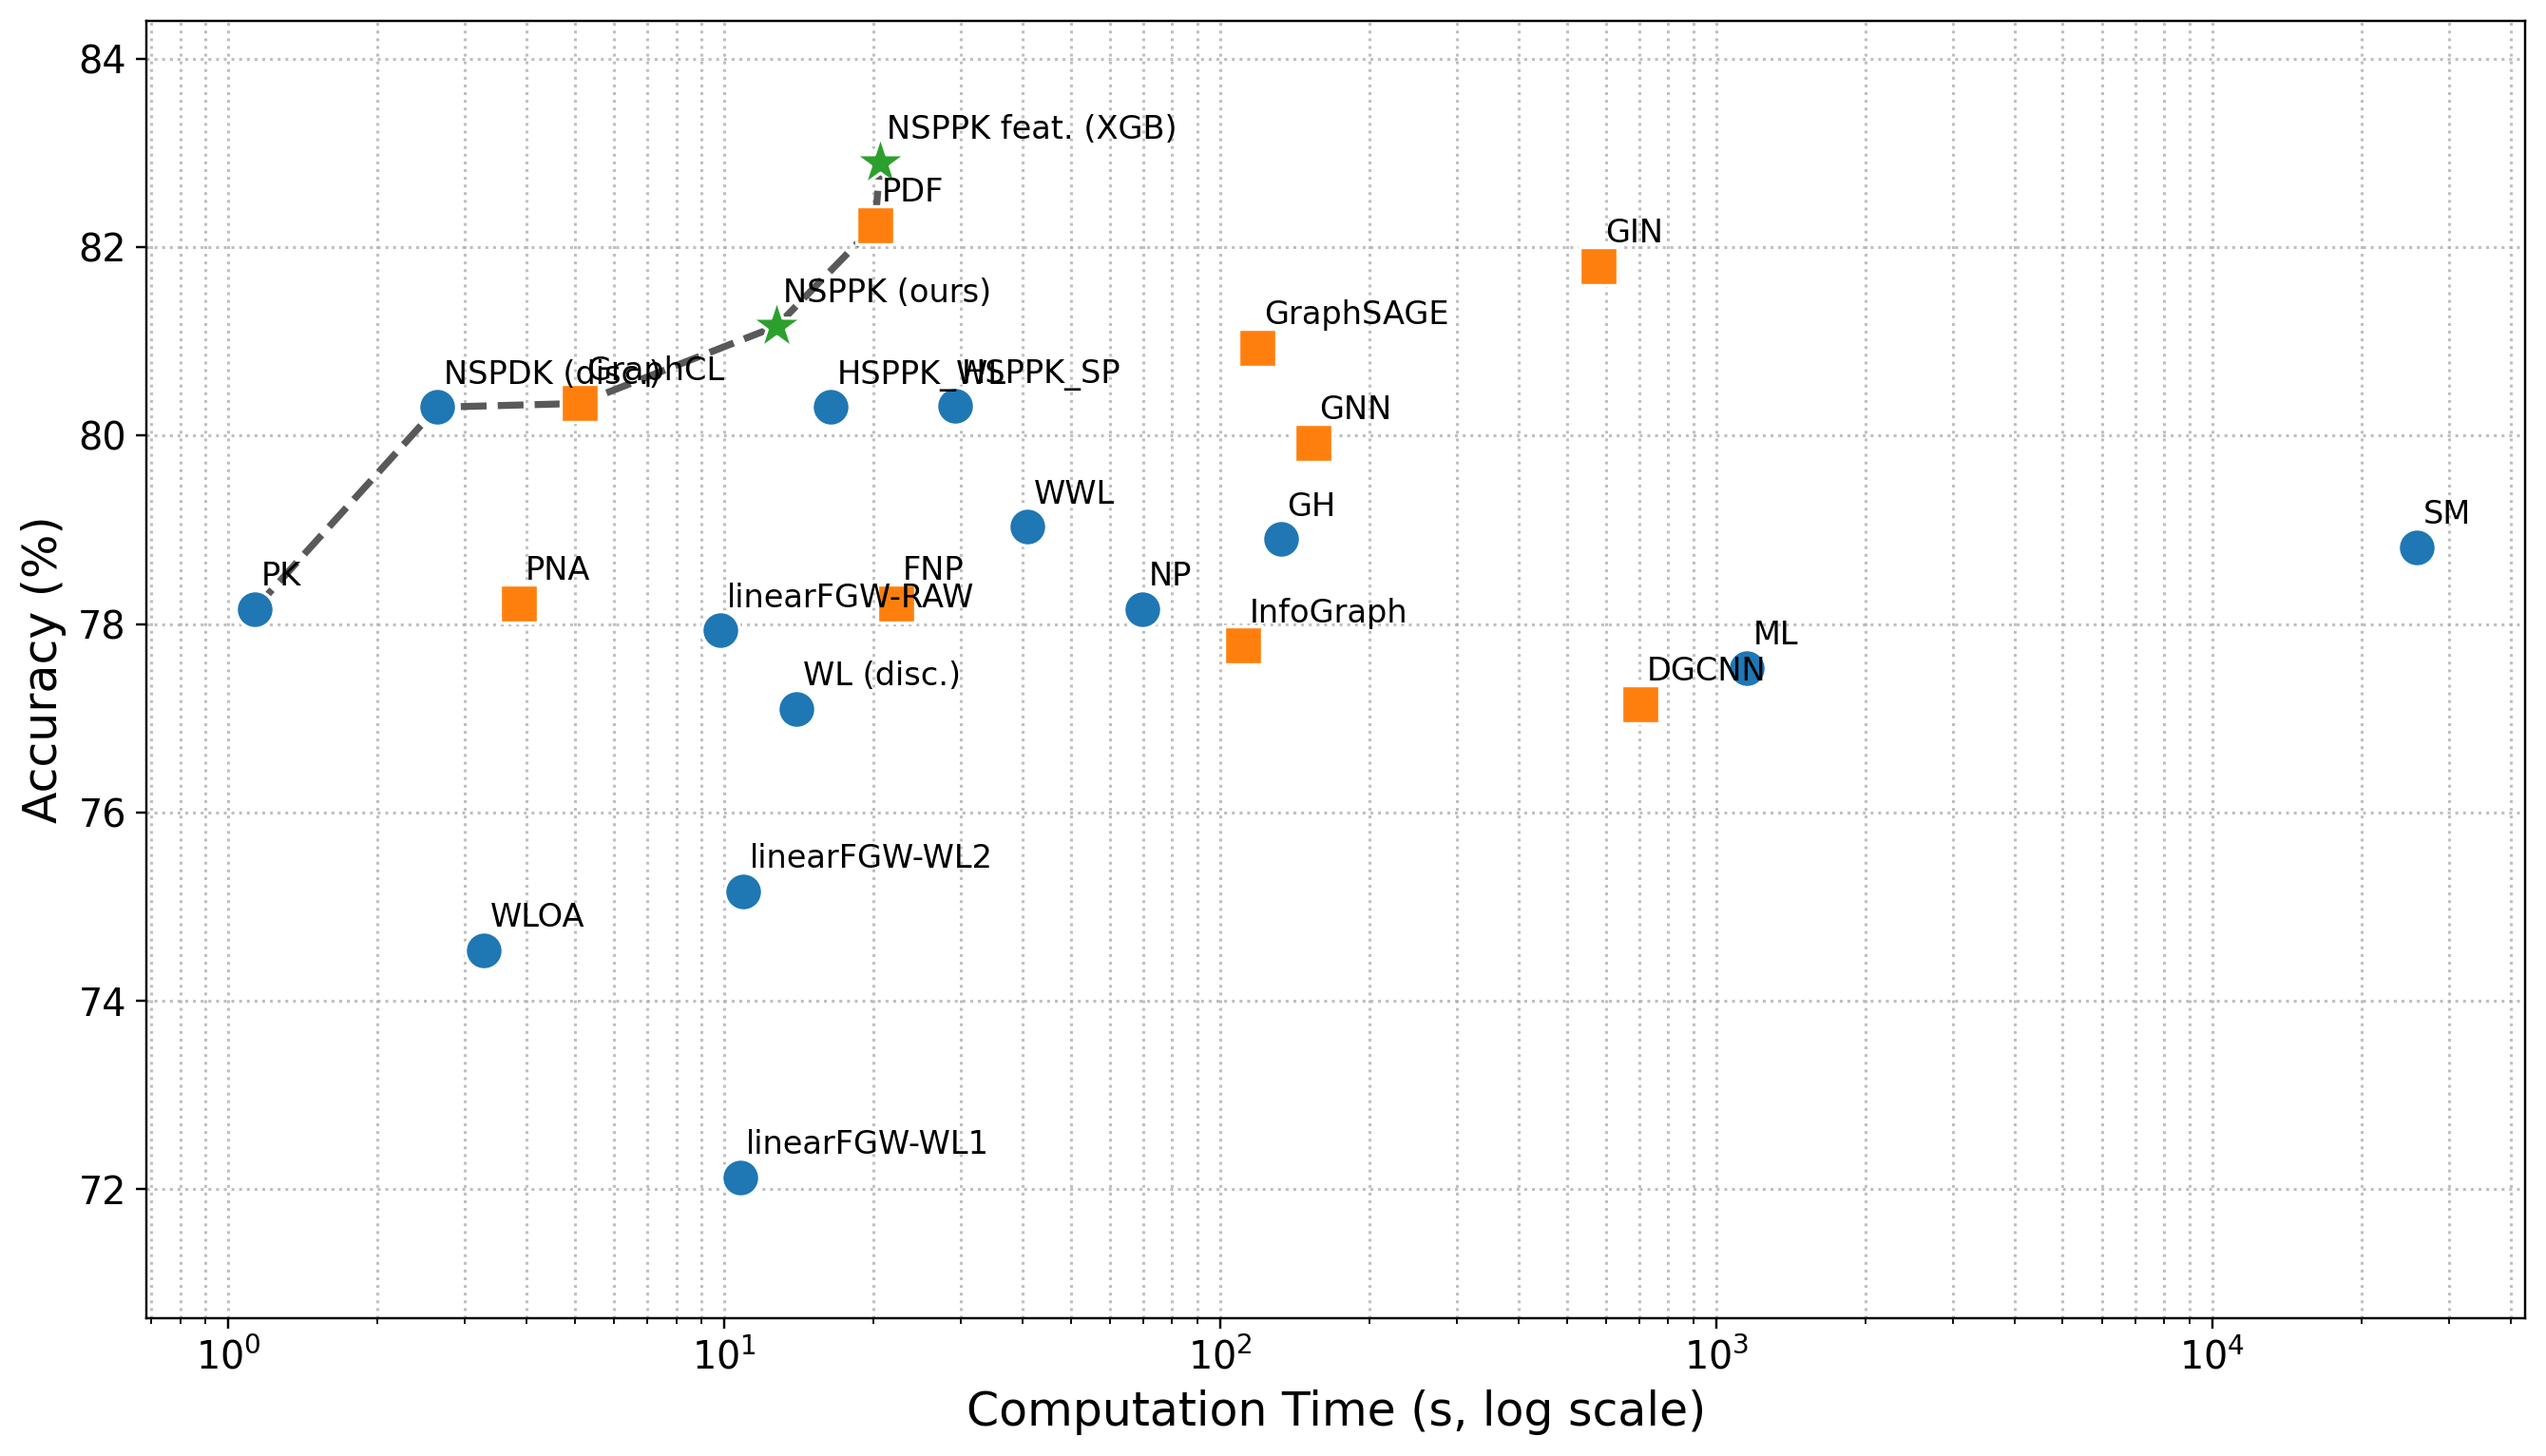
\includegraphics[width=\linewidth]{images/tradeoff_cox2.png}
  \caption{COX2}
\end{subfigure}

\vspace{3pt}

% ---------- bottom (full width) ----------
\begin{subfigure}[t]{0.98\textwidth}
  \centering
  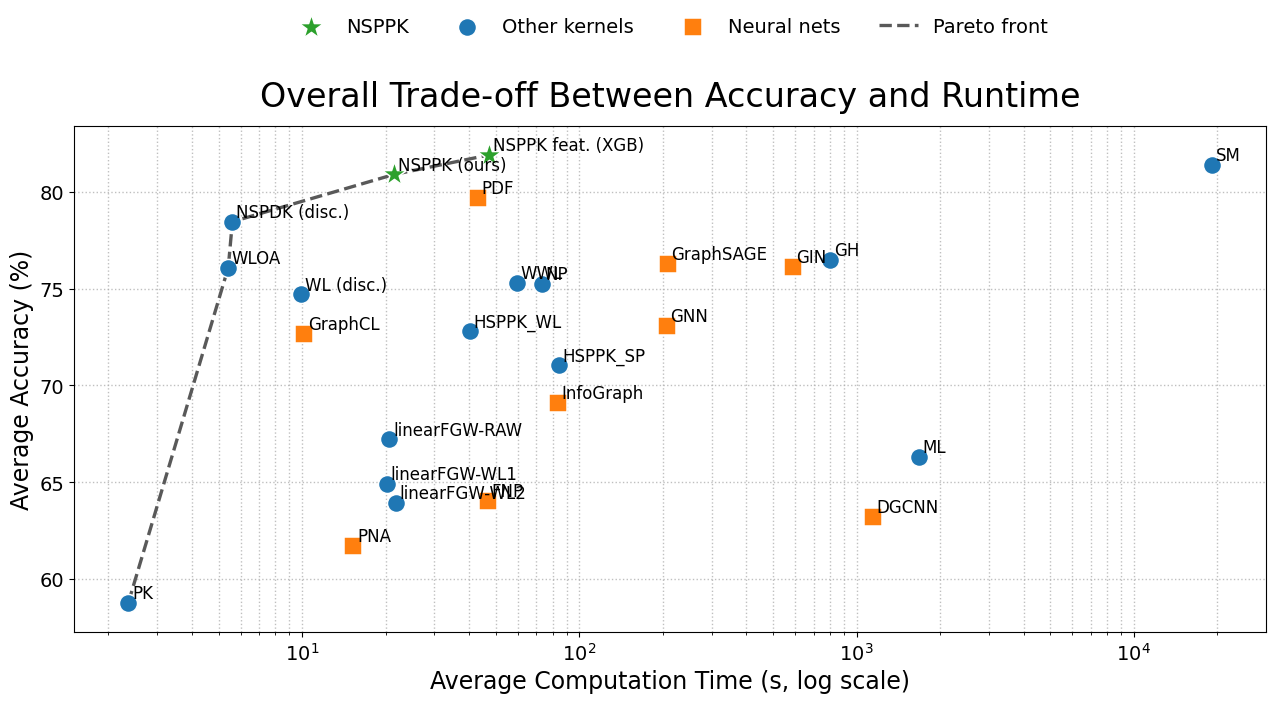
\includegraphics[width=\linewidth]{images/tradeoff_overall_average.png}
  \caption{Overall (average across datasets)}
\end{subfigure}

\caption{\textbf{Accuracy--time trade-off (log runtime).}
Markers denote method families: green star = NSPPK, blue circle = kernel
methods, orange square = neural networks. The dashed line indicates the
Pareto front.}
\label{fig:tradeoff_all}
\end{figure}

\paragraph{Summary.}
Figure~\ref{fig:tradeoff_all} shows that, for most datasets, NSPPK
(green star) lies on or close to the Pareto frontier. Methods are distributed
along the efficiency--accuracy spectrum: some are faster but less accurate,
while others achieve slightly higher accuracy at significantly greater
computational cost. In the aggregated panel, NSPPK remains on the global
frontier, indicating a favourable balance between predictive performance and
runtime.

\section{Additional Results in the No-Attribute Setting}
\label{appendix:no_attr}

To isolate the structural contribution of each method, we repeated the
graph classification experiments after removing all node attributes.
Tables~\ref{tab:no_attr} and~\ref{tab:nn_no_attr} report the resulting
classification accuracies for kernel and neural methods, respectively.
Overall, NSPPK remains competitive in this structural-only setting,
indicating that its performance does not depend solely on attribute
information and that it captures meaningful structural regularities.

% ========================= WITHOUT ATTRIBUTES =========================
\begin{table}[H]
\centering
\caption{Classification accuracy (\%) \textbf{without} node attributes, with average rank.}
\label{tab:no_attr}
\scriptsize
\setlength{\tabcolsep}{3.2pt}
\begin{adjustbox}{max width=\textwidth}
\begin{tabular}{lccccccc}
\toprule
\textbf{Method} & \makecell{SYNTHETIC\\new} & \textbf{DHFR} & \textbf{BZR} & \textbf{COX2} & \textbf{ENZYMES} & \textbf{PROTEINS} & \textbf{Avg Rank} \\
\midrule
SM  & \TO & \TO & \mps{79.02}{1.10} & \mps{78.16}{0.81} & \TO & \TO & 8.75 \\
SP  & \TO & \TO & \TO & \TO & \TO & \TO & -- \\
ML  & \mps{67.22}{9.51} & \mps{79.90}{1.36} & \mps{86.63}{3.81} & \mps{77.95}{4.63} & \mps{33.66}{5.31} & \mps{72.80}{3.80} & \textbf{4.17} \\
PK  & \mps{61.33}{7.33} & \mps{60.98}{0.48} & \mps{78.77}{1.01} & \mps{78.16}{8.07} & \mps{18.33}{5.22} & \mps{58.48}{4.29} & 10.83 \\
HSPPK\_WL & \mps{50.00}{0.00} & \mps{57.56}{6.67} & \mps{80.26}{3.02} & \mps{72.41}{17.06} & \mps{16.50}{2.73} & \mps{63.80}{5.76} & 11.17 \\
HSPPK\_SP & \mps{58.00}{7.18} & \mps{64.42}{4.05} & \mps{76.26}{9.39} & \mps{77.31}{4.70} & \mps{21.00}{5.92} & \mps{46.20}{4.70} & 11.67 \\
GH  & \mps{59.33}{9.28} & \mps{74.08}{4.27} & \mps{81.25}{2.40} & \mps{77.30}{3.14} & \mps{25.17}{3.98} & \mps{71.61}{4.32} & 7.17 \\
NP  & \mps{97.00}{3.15} & \mps{80.43}{4.01} & \mps{84.16}{5.65} & \mps{80.29}{3.42} & \mps{36.70}{0.53} & \mps{69.99}{3.88} & 5.17 \\
linearFGW-RAW & \mps{57.33}{6.29} & \mps{54.90}{4.77} & \mps{80.52}{3.76} & \mps{76.24}{4.74} & \mps{23.00}{4.88} & \mps{71.35}{4.56} & 8.33 \\
linearFGW-WL1 & \mps{56.00}{11.72} & \mps{63.90}{3.97} & \mps{80.99}{5.24} & \mps{76.45}{1.86} & \mps{24.50}{4.78} & \mps{70.17}{4.81} & 8.17 \\
linearFGW-WL2 & \mps{48.67}{7.33} & \mps{59.12}{6.41} & \mps{79.48}{5.48} & \mps{74.74}{5.12} & \mps{22.33}{5.59} & \mps{69.54}{3.12} & 9.50 \\
WL (disc.) & \mps{79.00}{12.39} & \mps{80.56}{5.29} & \mps{87.90}{3.92} & \mps{78.17}{3.48} & \mps{40.17}{7.54} & \mps{69.00}{4.08} & \textbf{3.83} \\
WLOA & \mps{81.00}{6.16} & \mps{80.96}{3.90} & \mps{83.71}{8.36} & \mps{78.16}{2.75} & \mps{42.67}{4.84} & \mps{74.49}{3.53} & 4.67 \\
WWL & \mps{50.00}{0.00} & \mps{60.98}{0.47} & \mps{78.77}{1.01} & \mps{78.16}{0.80} & \mps{16.67}{0.00} & \mps{55.57}{0.17} & 12.17 \\
NSPDK & \mps{95.33}{3.72} & \mps{82.94}{5.70} & \mps{85.68}{4.04} & \mps{77.09}{3.84} & \mps{35.67}{9.22} & \mps{71.33}{3.06} & 6.00 \\
NSPDK (disc.) & \mps{95.33}{3.72} & \mps{82.94}{5.70} & \mps{85.68}{4.04} & \mps{77.09}{3.84} & \mps{35.67}{9.22} & \mps{71.33}{3.06} & 6.00 \\
\rowcolor{gray!10}
\textbf{NSPPK (ours)} & \mps{98.00}{3.93} & \mps{80.18}{5.58} & \mps{87.65}{4.54} & \mps{77.73}{3.96} & \mps{33.17}{5.80} & \mps{71.34}{4.06} & \textbf{4.33} \\
\bottomrule
\end{tabular}
\end{adjustbox}

\vspace{0.5ex}
\footnotesize\emph{Note:} Average rank is computed over available entries only; lower is better. Timeouts and unavailable results are omitted on a per-dataset basis.
\end{table}

% ========================= NEURAL NETS — WITHOUT ATTRIBUTES =========================
\begin{table}[H]
\centering
\caption{Neural network classification accuracy (\%) \textbf{without} node attributes, with average rank.}
\label{tab:nn_no_attr}
\scriptsize
\setlength{\tabcolsep}{3.2pt}
\begin{adjustbox}{max width=\textwidth}
\begin{tabular}{lccccccc}
\toprule
\textbf{Method} &
\makecell{SYNTHETIC\\new} &
\textbf{DHFR} &
\textbf{BZR} &
\textbf{COX2} &
\textbf{ENZYMES} &
\textbf{PROTEINS} &
\textbf{Avg Rank} \\
\midrule
DGCNN     & \mps{44.67}{6.86} & \mps{61.50}{4.93} & \mps{81.98}{2.20} & \mps{78.22}{0.07} & \mps{26.80}{7.09} & \mps{73.22}{3.48} & 6.83 \\
GraphSAGE & \mps{43.33}{5.58} & \mps{78.06}{6.25} & \mps{83.70}{5.59} & \mps{80.30}{0.03} & \mps{48.17}{7.58} & \mps{74.93}{2.82} & 4.83 \\
InfoGraph & \mps{67.33}{21.54} & \mps{71.53}{8.51} & \mps{75.05}{15.04} & \mps{69.02}{0.20} & \mps{53.33}{4.79} & \mps{63.07}{4.69} & 5.50 \\
GIN       & \mps{53.00}{9.71} & \mps{79.91}{7.91} & \mps{73.95}{3.30} & \mps{79.91}{0.08} & \mps{42.67}{7.68} & \mps{65.77}{5.02} & 5.17 \\
GraphCL   & \mps{50.00}{8.69} & \mps{80.16}{2.51} & \mps{79.99}{3.62} & \mps{81.38}{3.79} & \mps{37.50}{5.12} & \mps{71.43}{3.92} & 4.00 \\
GNN       & \mps{43.33}{5.58} & \mps{82.67}{4.96} & \mps{84.66}{4.60} & \mps{81.60}{5.54} & \mps{48.50}{5.80} & \mps{71.79}{3.61} & 4.17 \\
FNP       & \mps{50.00}{8.69} & \mps{60.85}{4.63} & \mps{81.73}{3.52} & \mps{78.22}{3.94} & \mps{35.83}{7.79} & \mps{72.41}{3.70} & 5.00 \\
PNA       & \mps{46.00}{7.72} & \mps{60.98}{4.46} & \mps{78.76}{4.33} & \mps{78.22}{7.01} & \mps{18.83}{7.07} & \mps{70.62}{3.69} & 7.50 \\
PDF       & \mps{50.00}{8.69} & \mps{78.83}{4.21} & \mps{84.43}{4.63} & \mps{81.38}{3.79} & \mps{52.00}{5.26} & \mps{74.75}{2.28} & 3.67 \\
\rowcolor{gray!10}
NSPPK feat.\ (XGBoost)
          & \mps{91.00}{4.73} & \mps{78.44}{1.27} & \mps{89.60}{3.29} & \mps{82.76}{4.25} & \mps{41.83}{5.55} & \mps{71.60}{3.15} & \textbf{2.33} \\
\bottomrule
\end{tabular}
\end{adjustbox}
\end{table}

\section{Additional Runtime Results in the No-Attribute Setting}
\label{appendix:no_attr_runtime}

Tables~\ref{tab:no_attr_runtime_kernels} and~\ref{tab:no_attr_runtime_nns}
report computation times in the no-attribute setting for kernel and neural
methods, respectively. As expected, runtimes are generally lower once node
attributes are removed. Nevertheless, the relative efficiency trends remain
similar to those observed in the attributed setting, and NSPPK retains a
favourable balance between runtime and predictive performance.

% ========================= RUNTIMES: KERNELS (NO ATTRS) =========================
\begin{table}[H]
\centering
\caption{Kernel runtimes (seconds) \textbf{without} node attributes (\textbf{lower is better}).}
\label{tab:no_attr_runtime_kernels}
\scriptsize
\setlength{\tabcolsep}{3.5pt}
\begin{adjustbox}{max width=\textwidth}
\begin{tabular}{lcccccccc}
\toprule
\textbf{Method} & \textbf{SYNTH} & \textbf{DHFR} & \textbf{BZR} & \textbf{COX2} & \textbf{ENZ} & \textbf{PROT} & \textbf{Avg} & \textbf{Rank}\\
\midrule
SM & \TO & \TO & 11853.30\,s & 25478.50\,s & \TO & \TO & 18665.90\,s & 16.00\\
SP & \TO & \TO & \TO & \TO & \TO & \TO & -- & --\\
ML & 978.86\,s & 1300.05\,s & 158.40\,s & 1509.62\,s & 1792.43\,s & 5661.68\,s & 1900.17\,s & 15.00\\
PK & 0.59\,s &  0.66\,s & 0.23\,s & 0.33\,s & 0.78\,s & 2.11\,s & 0.78\,s & 2.00\\
HSPPK\_WL & 38.74\,s & 29.97\,s & 8.76\,s & 11.30\,s & 19.83\,s & 76.69\,s & 30.88\,s & 10.00\\
HSPPK\_SP & 285.63\,s & 137.62\,s & 18.33\,s & 25.21\,s & 31.37\,s & 121.37\,s & 103.26\,s & 12.17\\
GH & 178.47\,s & 322.97\,s & 99.82\,s & 132.87\,s & 365.25\,s & 791.82\,s & 315.20\,s & 13.83\\
NP & 66.93\,s & 279.77\,s & 44.90\,s & 97.51\,s & 69.69\,s & 240.32\,s & 133.19\,s & 12.83\\
linearFGW-RAW & 6.21\,s & 19.98\,s & 6.17\,s & 8.75\,s & 12.91\,s & 76.17\,s & 21.70\,s & 7.67\\
linearFGW-WL1 & 7.00\,s & 20.01\,s & 6.24\,s & 10.22\,s & 8.51\,s & 52.96\,s & 17.49\,s & 7.67\\
linearFGW-WL2 & 6.17\,s & 25.21\,s & 5.21\,s & 11.27\,s & 11.82\,s & 74.40\,s & 22.35\,s & 7.50\\
WL (disc.) & 0.14\,s & 0.25\,s & 0.05\,s & 0.12\,s & 0.13\,s & 0.34\,s & 0.17\,s & \textbf{1.00}\\
WLOA & 0.96\,s & 5.08\,s & 0.95\,s & 1.37\,s & 3.32\,s & 8.19\,s & 3.31\,s & 4.17\\
WWL & 13.19\,s & 79.33\,s & 11.17\,s & 29.40\,s & 24.10\,s & 90.97\,s & 41.36\,s & 11.00\\
NSPDK & 5.78\,s & 4.26\,s & 3.07\,s & 2.81\,s & 2.24\,s & 3.11\,s & 3.55\,s & 4.00\\
NSPDK (disc.) & 5.78\,s & 4.26\,s & 3.07\,s & 2.81\,s & 2.24\,s & 3.11\,s & 3.55\,s & 4.00\\
\rowcolor{gray!10}
\textbf{NSPPK (ours)} & 11.31\,s & 34.55\,s & 6.09\,s & 6.09\,s & 5.58\,s & 4.72\,s & 11.39\,s & 7.17\\
\bottomrule
\end{tabular}
\end{adjustbox}
\end{table}

% ========================= RUNTIMES: NEURAL (NO ATTRS) =========================
\begin{table}[H]
\centering
\caption{Neural runtimes (seconds) \textbf{without} node attributes (\textbf{lower is better}).}
\label{tab:no_attr_runtime_nns}
\scriptsize
\setlength{\tabcolsep}{3.5pt}
\begin{adjustbox}{max width=\textwidth}
\begin{tabular}{lcccccccc}
\toprule
\textbf{Method} & \textbf{SYNTH} & \textbf{DHFR} & \textbf{BZR} & \textbf{COX2} & \textbf{ENZ} & \textbf{PROT} & \textbf{Avg} & \textbf{Rank}\\
\midrule
DGCNN & 428.69\,s & 575.14\,s & 571.26\,s & 237.85\,s & 887.36\,s & 1611.41\,s & 718.62\,s & 9.83\\
GraphSAGE & 124.81\,s & 109.79\,s & 126.21\,s & 140.69\,s & 248.03\,s & 395.38\,s & 190.82\,s & 7.50\\
InfoGraph & 65.27\,s & 185.02\,s & 100.00\,s & 87.92\,s & 144.01\,s & 241.47\,s & 137.28\,s & 6.33\\
GIN & 388.95\,s & 392.46\,s & 358.57\,s & 392.46\,s & 440.30\,s & 884.01\,s & 476.12\,s & 9.17\\
GraphCL & 3.58\,s & 13.53\,s & 4.23\,s & 5.42\,s & 13.28\,s & 17.61\,s & 9.61\,s & 1.83\\
GNN & 81.93\,s & 255.75\,s & 28.95\,s & 122.86\,s & 247.42\,s & 403.82\,s & 190.12\,s & 7.00\\
FNP & 7.69\,s & 92.75\,s & 63.45\,s & 15.82\,s & 70.24\,s & 38.84\,s & 48.13\,s & 4.33\\
PNA & 3.32\,s & 19.04\,s & 3.83\,s & 2.80\,s & 8.59\,s & 23.63\,s & 10.20\,s & \textbf{1.50}\\
PDF & 13.12\,s & 75.36\,s & 17.80\,s & 23.45\,s & 63.85\,s & 67.34\,s & 43.49\,s & 4.50\\
NSPPK feat.\ (XGB) & 32.91\,s & 10.07\,s & 4.28\,s & 6.25\,s & 7.43\,s & 60.64\,s & 20.26\,s & 3.00\\
\bottomrule
\end{tabular}
\end{adjustbox}
\end{table}

\chapter{Summary and Conclusion}
\label{ch:conclusion}

\section{Summary of Contributions}
\label{sec:conclusion:summary}

This thesis developed methods for representing, generating, and evaluating
graphs. The work was motivated by a common difficulty across these tasks:
graphs are irregular, permutation-sensitive, and often constrained by
domain-specific validity requirements. A useful method must therefore preserve
graph structure, remain inspectable where possible, and support reliable
comparison when used inside a generative pipeline.
The thesis made three main contributions.

\textbf{NSPPK for interpretable graph representation.}
The first contribution was the Neighborhood Subgraph Pairwise Path Kernel
(NSPPK), an explicit graph-to-vector representation for node-attributed graphs. For
each graph, NSPPK constructs a sparse feature vector by enumerating structural
patterns around pairs of nodes. Each feature records the neighbourhoods around the nodes together with the shortest-path subgraph that connects them. In this way, the representation captures both local node-centred structure and the broader context linking different parts of the graph.
Continuous node attributes are incorporated directly into these explicit
features, avoiding discretisation while retaining deterministic, sparse, and
interpretable feature construction.

Empirically, NSPPK showed that carefully designed explicit representations can
remain competitive with learned graph neural models, especially in low-data or
sample-efficient regimes. Its sparse feature map also supports computationally
transparent downstream learning and enables predictive behaviour to be related
back to structural graph patterns.

\textbf{GCDG for graph-conditioned generation.}
The second contribution was the Graph-Conditioned Diffusion Generator (GCDG), a
conditional graph generator that uses graph-level vectors to guide the
generation of node-level representations. The central contribution is the
graph-level-to-node-level conditional generation formulation: a fixed
graph-level descriptor conditions the generation of a padded node-level feature
matrix, from which the final graph is decoded. The diffusion process is defined
over continuous node-level features, while the denoising network predicts the
clean node representation and latent states used by downstream prediction
modules. These modules estimate node presence, node labels, degree-related
information, edge probabilities, and edge labels where available. A
constraint-aware decoder then combines the node-level and pairwise predictions
to construct the final discrete graph.

This  design makes the generation process more inspectable than a single
black-box graph decoder. Intermediate quantities such as node-existence
probabilities, edge scores, degree predictions, and label predictions can be
examined before the final graph is selected. Experiments on synthetic
cycle--leg graphs and QM9 molecular graphs showed that conditioning quality and
graph validity are distinct issues: a model may produce plausible graphs while
failing to preserve the requested conditional structure. The chapter therefore
emphasised generation as conditional graph construction rather than
unconditional sampling alone.

\textbf{RankGen for statistically grounded evaluation.}
The third contribution was RankGen, a classifier-based framework for evaluating
generative models. RankGen treats evaluation as a collection of predictive
probes rather than as a single scalar similarity computation. The framework
defines four complementary metrics: Quality, Utility, Indistinguishability,
and Similarity, together with a composite score, Exchangeability. These metrics
diagnose different failure modes, including poor
task fidelity, lack of augmentation value, distributional separability, local
structural mismatch, and memorisation.

RankGen combines these probes with PAC-style finite-sample reliability
bounds and robust quantile-based aggregation. This separates the question of
whether a comparison is statistically reliable from the question of which
reliable model should be ranked higher. Experiments across controlled
perturbations, molecular graph
generators, image benchmarks, and open-domain text generation demonstrated that
the framework can expose behaviours that conventional metrics often collapse
or obscure.

\section{Key Insights and Lessons Learned}
\label{sec:conclusion:insights}

Several broader lessons emerge from these contributions.

First, explicit graph representations remain valuable. Although neural graph
models are highly expressive, deterministic feature maps can provide strong
performance, favourable sample efficiency, and clearer interpretability. NSPPK
shows that the limitations of classical kernels are not inherent to explicit
representations themselves; they can be addressed by enriching the structural
features and by treating continuous attributes directly.

Second, graph generation benefits from separating modelling roles. In GCDG, the
diffusion model is not asked to solve every part of graph generation at once.
Continuous structural representations, categorical node labels, edge
prediction, and final constraint satisfaction are handled by different
components. This separation does not remove the difficulty of graph generation,
but it makes the source of successes and failures easier to inspect.

Third, conditional generation must be evaluated conditionally. It is not enough
for a generated graph to look plausible under aggregate statistics. If the
generator receives a graph-level condition, then the generated graph should be
tested against the information encoded in that condition. The synthetic
cycle--leg experiments illustrate this point clearly: different models can fail
in different conditional regimes even when their outputs remain graph-like.

Fourth, generative model evaluation is inherently multi-dimensional. A
generator may preserve predictive signal but be distributionally
distinguishable; it may generate realistic-looking samples that add little
utility; or it may perform well under global metrics while failing local
mixing or memorisation checks. RankGen addresses this by treating evaluation as
a structured statistical problem rather than a search for one universal score.

\section{Limitations}
\label{sec:conclusion:limitations}

The work in this thesis also has limitations.

For NSPPK, the use of explicit substructure enumeration provides
interpretability but can become expensive on dense or very large graphs. The
method is designed around bounded radii and distances, so its practical
scalability depends on parameter choices and graph density. The feature hashing
pipeline is efficient and deterministic, but hashed representations can still
merge distinct patterns when the hash space is limited. In addition, NSPPK
captures structural information through predefined features rather than
learning task-specific representations end-to-end.

For GCDG, the  architecture introduces dependencies between components.
If the node representation does not preserve information needed for decoding,
the constrained decoder cannot recover it later. Conversely, a strong decoder or domain-specific constraint can improve validity,
but it also makes it harder to determine how much of the final performance
comes from the learned generator and how much comes from post-processing. 
than as a complete molecular-design benchmark.

For RankGen, the framework depends on the quality of the chosen classifiers,
feature representations, and resampling protocol. Classifier-based evaluation
is powerful because it connects generation to predictive tasks, but it also
inherits the biases and limitations of the classifiers and embeddings used.
The PAC-style bounds provide conservative reliability checks, yet they do not
eliminate all sources of experimental variability. RankGen should therefore be
viewed as a diagnostic framework rather than as a replacement for all
domain-specific evaluation.

Across the thesis, a further limitation is that the strongest claims are made
within the graph and benchmark settings studied here. Across the thesis, a further limitation concerns the scope of the evaluation
formalism. RankGen is developed primarily around supervised, classifier-based
probes, where predictive accuracy and real-versus-generated discrimination
provide natural diagnostic signals. Extending the framework to regression
tasks, unsupervised learning, or settings without reliable labels would require
additional formal development, including appropriate probe definitions,
uncertainty bounds, and criteria for task-relevant utility.

\section{Future Research Directions}
\label{sec:conclusion:future}

Several directions follow naturally from this work.

\textbf{Hybrid explicit and neural representations.}
NSPPK suggests that explicit graph features can provide useful structural
signals. A promising direction is to combine such features with neural graph
models, either as input channels, regularisers, attention biases, or
interpretable probes for learned embeddings. This could preserve the
sample-efficiency and auditability of kernels while benefiting from the
task-specific flexibility of neural representation learning.

\textbf{Scalable conditional graph generation.}
Future work on GCDG could improve scalability to larger and denser graphs by
developing more efficient decoding procedures, sparse pairwise prediction, and
hierarchical generation. Another direction is to learn constraint handling more
closely with the denoising process, reducing the gap between neural generation
and final feasibility projection while retaining inspectability.

\textbf{Richer condition preservation metrics.}
Conditional generation requires evaluation methods that compare generated
objects not only to a population, but also to the specific condition that
produced them. Future work could extend RankGen-style probes to conditional
settings by measuring condition-response fidelity, conditional diversity, and
the stability of generated samples under controlled changes to the condition
vector.

\textbf{Evaluation under privacy and safety constraints.}
RankGen already addresses memorisation as a diagnostic concern, but future work
could connect the framework more directly to privacy auditing, extraction
risk, and safety-sensitive deployment. This is especially important in domains
where generated data may contain sensitive information or where synthetic data
is used to support downstream decisions.

\textbf{Application-specific scientific validation.}
For molecular and other scientific graph domains, further validation should
include stronger domain-specific constraints, expert-defined utility criteria,
and prospective testing. Distributional similarity is useful, but scientific
generators ultimately need to support discovery, optimisation, or reliable
simulation in the target domain.

\section{Closing Remarks}
\label{sec:conclusion:closing}

The central message of this thesis is that effective and trustworthy graph
generation requires more than a powerful sampler. It requires representations
that expose relevant graph structure, generators whose intermediate decisions
can be inspected, and evaluation protocols that distinguish genuine utility
from surface-level similarity.

NSPPK, GCDG, and RankGen address these three parts of the problem. NSPPK shows
that explicit graph structure can be represented in a sparse and interpretable
form, including continuous attributes. GCDG shows how such graph-level
information can guide a staged denoising generator for discrete graphs. RankGen
shows how generated data can be assessed through statistically grounded,
diagnostic probes.

Taken together, the contributions support a broader view of graph generative
modelling: representation, generation, and evaluation should be designed
together. When these components are aligned, generated graphs can be assessed
not only by whether they appear plausible, but by whether they preserve
meaningful structure, satisfy relevant constraints, and provide reliable value
for downstream use.

\chapter{Supplementary Material for Chapter 5: RankGen}
\label{appendix:ch5}
\label{app:theory-metric-defs}


\label{appendix:bounds}

\begin{table}[H]
\centering

\label{tab:notation-glossary}
\vspace{-1.5em}

\footnotesize
\setlength{\tabcolsep}{5pt}
\renewcommand{\arraystretch}{1}

\resizebox{\textwidth}{!}{%
\begin{tabular}{@{}p{3.1cm}p{2.2cm}p{9.2cm}@{}}
% \toprule
\textbf{Symbol} & \textbf{Type} & \textbf{Meaning / definition} \\
\midrule

\multicolumn{3}{@{}l}{\emph{Datasets and sample sizes}}\\
$D_{\text{train1}}^{(i)}$ & set & Real training subset used for the baseline classifier.\\
$D_{\text{train2}}^{(i)}$ & set & Additional real data used for the upper-bound classifier.\\
$D_{\text{generated}}^{(i)}$ & set & Generated data produced by the generator.\\
$D_{\text{test}}$ & set & Held-out real test set used for evaluation.\\
$D_{\mathrm r},\;D_{\mathrm g}$ & sets & Real and generated sample sets in the similarity setting.\\
$D_{\text{mix}}^{(i)}$ & set & Mixed pool $D_{\text{train1}}^{(i)} \cup D_{\text{generated}}^{(i)}$ used to measure local mixing.\\
$n,\;n_r,\;n_g$ & scalars & Total, real, and generated sample sizes, with $n=n_r+n_g$.\\
$m$ & scalar & Size of the balanced discriminator/domain-classifier pool.\\
$k$ & scalar & Number of nearest neighbours in the similarity metric.\\
$P_r,\;P_g$ & distributions & Real data distribution and generated data distribution.\\

\midrule
\multicolumn{3}{@{}l}{\emph{Model classes}}\\
$\Phi_\theta$ & map & Task classifier architecture.\\
$\Psi_\theta$ & map & Real-vs-generated discriminator.\\
$\Gamma_\theta$ & map & Helper used to compute the similarity statistic.\\

\midrule
\multicolumn{3}{@{}l}{\emph{Raw classifier accuracies}}\\
$\rho_1^{(i)}$ & num. & Task score using $\Phi_\theta$ trained on $D_{\text{train1}}^{(i)}$ only.\\
$\rho_2^{(i)}$ & num. & Task score using $\Phi_\theta$ trained on $D_{\text{generated}}^{(i)}$ only.\\
$\rho_3^{(i)}$ & num. & Task score using $\Phi_\theta$ trained on $D_{\text{train1}}^{(i)} \cup D_{\text{train2}}^{(i)}$.\\
$\rho_4^{(i)}$ & num. & Task score using $\Phi_\theta$ trained on $D_{\text{train1}}^{(i)} \cup D_{\text{generated}}^{(i)}$.\\
$\rho_5^{(i)}$ & num. & Discriminator accuracy for distinguishing real from generated samples.\\
$\rho_6^{(i)}$ & num. & Raw similarity statistic used to construct $S^{(i)}$.\\
$\rho_j^\star$ & num. & Population counterpart of $\rho_j^{(i)}$.\\

\midrule
\multicolumn{3}{@{}l}{\emph{Derived quantities}}\\
$\Delta_{\text{real}}^{(i)}$ & num. & $\rho_3^{(i)}-\rho_1^{(i)}$, gain from adding more \emph{real} data.\\
$\Delta_{\text{generated}}^{(i)}$ & num. & $\rho_4^{(i)}-\rho_1^{(i)}$, gain from adding \emph{generated} data.\\
$\gamma^\star$ & num. & $|R_Q(h_s)-R_Q(h_{r'})|$, generated-domain gap between $h_s$ and $h_{r'}$.\\
$Q^{(i)}$ & num. & Empirical quality score on split $i$.\\
$Q^\star$ & num. & Population quality score.\\
$U^{(i)}$ & num. & Empirical utility score on split $i$.\\
$U^\star$ & num. & Population utility score.\\
$I^{(i)}$ & num. & Empirical indistinguishability score on split $i$.\\
$I^\star$ & num. & Population indistinguishability score.\\
$S^{(i)}$ & num. & Empirical similarity score on split $i$.\\
$S^\star$ & num. & Population similarity score.\\
$\mathcal E_{\min}^{(i)}$ & num. & Empirical exchangeability score on split $i$.\\
$\mathcal E_{\min}^\star$ & num. & Population exchangeability score.\\

\midrule
\multicolumn{3}{@{}l}{\emph{Error terms and constants in PAC bounds}}\\
$\varepsilon_{\mathrm{gen}}$ & bnd. & Test-accuracy sampling/generalisation error term.\\
$\varepsilon_{\mathrm{disc}}$ & bnd. & Discrepancy estimation error term.\\
$\varepsilon_{\mathrm{syn}},\;\varepsilon_{\mathrm{real}}$ & bnd. & Composite errors for $\Delta_{\text{generated}}$ and $\Delta_{\text{real}}$.\\
$\varepsilon_{\mathrm{sim}}$ & bnd. & Error radius for the similarity metric.\\
$\mathcal R_n$ & scalar & Rademacher complexity of the classifier class.\\
$d$ & scalar & VC dimension upper bound for the discriminator class.\\
$L_H$ & scalar & Lipschitz constant of binary entropy on $[\tfrac1{k+1},1-\tfrac1{k+1}]$.\\
$\lambda$ & num. & Joint optimal risk term in the domain-adaptation bound.\\
$\delta$ & scalar & Confidence parameter, so bounds hold with probability at least $1-\delta$.\\

% \bottomrule
\end{tabular}%
}
\caption{Glossary of symbols used in the formal definitions and PAC guarantees of \textsc{RankGen}. A superscript $(i)$ denotes the $i$-th resampling split, a hat $\widehat{\phantom{x}}$ denotes an empirical finite-sample estimate when used, and a star ${}^\star$ denotes the corresponding population quantity.}
\end{table}
\section{Notation and Formal Metric Definitions}
\label{app:theory}

This appendix consolidates the formal definitions, assumptions, and PAC-style
bounds underlying the \textsc{RankGen} framework. Starred quantities denote
population-level quantities and are not estimated directly in practice; the
bounds are used only as conservative statistical gates on empirical scores.

We emphasize that the PAC-style bounds used in \textsc{RankGen} are intentionally
conservative and should not be interpreted as tight estimators of population
performance. In particular, capacity terms and Rademacher-style bounds are used
as engineering surrogates for statistical gating rather than as theoretically
exact certificates. This design reflects a deliberate choice: the role of the
bounds is to function as fail-safe rejection criteria, not as accuracy
estimators. Consequently, the pass/fail mechanism follows a Neyman--Pearson-style
logic---prioritizing control of false acceptance over tightness---so that
statistically unreliable models are filtered out, while passing merely indicates
that a model has not been ruled out with high confidence. This conservative bias
may reject some acceptable models, but avoids endorsing generators whose
empirical performance is not statistically supported.



\subsection{Formal Metric Definitions}

Using the notation above, the \textsc{RankGen} metrics on split $i$ are defined as
\begin{align}
Q^{(i)} &:= \min\!\left(\frac{\rho_2^{(i)}}{\rho_1^{(i)}},\,1\right),\\
U^{(i)} &:= \min\!\left\{1,\;\max\!\left\{0,\;\frac{\Delta_{\text{generated}}^{(i)}}{\Delta_{\text{real}}^{(i)}}\right\}\right\},\\
I^{(i)} &:= 1 - 2\bigl|\rho_5^{(i)} - 0.5\bigr|.
\end{align}
For similarity, define the mixed pool
\[
D_{\text{mix}}^{(i)} := D_{\text{train1}}^{(i)} \cup D_{\text{generated}}^{(i)},
\]
attach a binary domain label to each point, let $\hat p_x$ be the fraction of
same-domain neighbours among its $k$-nearest neighbours in $D_{\text{mix}}^{(i)}$,
and define the binary entropy
\[
H(p) := -p\log p -(1-p)\log(1-p).
\]
Then
\begin{equation}
S^{(i)} :=
\frac{1}{n}
\sum_{x\in D_{\text{mix}}^{(i)}}
\frac{H(\hat p_x)}{\log 2}.
\end{equation}
Finally, define the predictive and distributional blocks
\[
\Delta_{\text{qual}}^{(i)}=\tfrac12\bigl(Q^{(i)}+U^{(i)}\bigr),
\qquad
\Delta_{\text{sim}}^{(i)}=\tfrac12\bigl(I^{(i)}+S^{(i)}\bigr),
\]
and the exchangeability score
\begin{equation}
\mathcal{E}_{\min}^{(i)}
= \min\!\left\{\Delta_{\text{qual}}^{(i)},\,\Delta_{\text{sim}}^{(i)}\right\}.
\end{equation}

\section{PAC Assumptions and Bound Ingredients}
\label{app:theory-assumptions}

\subsection{Bound Ingredients and Assumptions}
\label{app:bound-ingredients}

For completeness, we collect the constants, estimators, and confidence allocations used in the PAC-style bounds from Sec.~\ref{sec:method}. This material is supplementary; the main text states only the bound forms. Some capacity terms are instantiated via conservative heuristics for practical gating and should therefore be interpreted as engineering surrogates rather than tight theoretical certificates.

\paragraph{Confidence allocation.}
Unless otherwise noted, we set $\delta_*=\delta/(MTB)$, where $M$ is the number
of models, $T$ the number of metrics, and $B$ the number of resampling splits. Each individual bound then holds with probability at least $1-\delta_*$, and all bounds jointly hold with probability at least $1-\delta$ by a union bound.

\paragraph{Quality.}
We use a standard domain-adaptation inequality with $P$ the real distribution and $Q$ the generated distribution to control $R_P(\hat h_g)$ through $R_Q(\hat h_g)$, the discrepancy term $\tfrac12\mathrm{disc}_{\mathcal H\Delta\mathcal H}(P,Q)$, and the joint optimal risk $\lambda$~\citep{ben2010theory,blitzer2007biographies}. The discrepancy is estimated by a balanced domain classifier, and $R_Q(\hat h_g)$ is estimated on a generated hold-out split so that uniform-convergence bounds apply. We assume $\rho_1^{(i)}>0$ for the ratio form; if $\rho_1^{(i)}$ is near zero, we revert to a difference form.

\paragraph{Utility.}
We again use the $\mathcal H\!\Delta\!\mathcal H$ discrepancy. Its empirical estimator is defined using a balanced domain classifier, with constants aligned to the definition in \eqref{eq:DA}. We compute
\[
\widehat\lambda = \min_{h\in\Phi_\theta}\widehat R_{D_{\mathrm r}'}(h)+\widehat R_{D_{\mathrm s}}(h)
\]
on an auxiliary split disjoint from the evaluation pool, and
\[
\hat\gamma=|\hat R_Q(h_s)-\hat R_Q(h_{r'})|
\]
on a generated hold-out pool, using cross-fitting if needed. If
$\Delta_{\text{real}}^{(i)}<\tau$ with $\tau=10^{-3}$, we use the difference utility $\Delta_{\text{generated}}^{(i)}$; otherwise we form the ratio $U^{(i)}$.

\paragraph{Indistinguishability.}
We apply a VC generalisation bound for the discriminator on a balanced pool and then use the $2$-Lipschitz property of $g(a)=1-2|a-0.5|$ to transfer the error in discriminator accuracy to the indistinguishability score.

\paragraph{Similarity.}
Neighbourhood label proportions are sampled without replacement, so we use Serfling-type concentration bounds for hypergeometric draws~\citep{serfling1974}. Restricting $p\in[1/(k+1),\,1-1/(k+1)]$ yields
\[
L_H=\log\!\tfrac{1-\tau}{\tau}=O(\log k),
\qquad \tau=\tfrac1{k+1},
\]
so the dependence on $k$ is explicit. A union bound over $n$ points gives the stated
$O(\sqrt{\log(n/\delta)/k})$ rate without requiring independence across points.

\paragraph{Composite.}
We set $\delta_Q=\delta_U=\delta_I=\delta_S=\delta/4$ so that the exchangeability bound holds with confidence at least $1-\delta$ by a union bound.

\subsection{Practical Capacity Choices for the PAC Bounds}
\label{app:bound-implementation}

In our experiments, we do not attempt to estimate data-dependent Rademacher complexities or exact VC dimensions for each classifier. Instead, following standard PAC practice, we use simple conservative analytic upper bounds that make the guarantees easy to implement and reproduce.

\paragraph{Rademacher complexity for the Quality bound.}
The quality bound requires an upper bound on the empirical Rademacher complexity $\mathcal{R}_n$ of the task-classifier class. We use the following rule:
\begin{itemize}
    \item If an upper bound $d$ on the VC dimension is supplied, we use the classical VC-based inequality
    \[
      \mathcal{R}_n \;\le\;
      \sqrt{\frac{2 d \log(e n / d)}{n}},
    \]
    which follows from the Sauer--Shelah lemma and standard symmetrization.
    \item If no VC bound is supplied, we use the heuristic gate
    \[
      \widetilde{\mathcal{R}}_n := \sqrt{\frac{2}{n}},
    \]
    as a conservative engineering surrogate. This quantity is \emph{not} a universal upper bound on $\mathcal R_n$ and is not a distribution-free PAC certificate; a formal guarantee requires an explicit capacity assumption.
\end{itemize}

For the synthetic experiments, we optionally allow a small model-specific constant $\mathcal{R}_n$ (e.g., $0.01$--$0.09$) as a capacity surrogate for each classifier family. These values are chosen to be no larger than the heuristic $\sqrt{2/n}$ gate and are used only as practical surrogates, not as theoretical certificates. Their effect is merely to make the gate slightly tighter or looser; the qualitative patterns reported are stable across a wide range of such constants.

\paragraph{VC dimension for discriminators in Utility and Indistinguishability.}
The utility and indistinguishability bounds require a capacity term for the real-vs-generated discriminator class. Since exact VC dimensions for modern ensembles are difficult to compute, we set a single conservative upper bound $d_{\mathrm{disc}} = 50$ for all discriminators. This value is passed to the bound functions as a hyperparameter; larger choices only weaken the bounds.

If $d_{\mathrm{disc}}$ is set to \texttt{None}, our implementation reverts to a Hoeffding-type deviation bound depending only on the number of evaluation examples $m$,
\[
  \varepsilon(m, \delta)
  = \sqrt{\frac{\log(2/\delta)}{2m}},
\]
which yields a distribution-free deviation bound for the fixed trained discriminator, at the cost of additional looseness.

\paragraph{Role of these constants.}
Across experiments, these capacity terms are used only to construct binary pass/fail gates for each generator--metric pair rather than to provide tight numerical certificates. Once a model passes the gate, ordering is based on robust quantile summaries (median/IQR) as described in Sec.~\ref{sec:quantile-based-estimation}. We verified that the qualitative conclusions are stable under reasonable variations of the capacity parameters.

\paragraph{Quantile-to-moment mapping.}
For ranking procedures that expect a mean and variance, we convert the empirical quartiles $(Q_1,M,Q_3)$ into a pseudo-mean and pseudo-standard deviation using the quantile-to-moment rules of \citet{wan2016estimatingsamplemeanstandard}:
\[
\hat{\mu}_Q = \tfrac{Q_1 + M + Q_3}{3},
\qquad
\hat{\sigma}_Q = \frac{\mathrm{IQR}}{1.34898}.
\]

\section{Quality Bound}
\label{app:theory-quality}
\label{appendix:quality-bound}

The quality score measures how closely a classifier trained on generated data matches the performance of one trained on real data:
\begin{equation}
Q^{(i)} = \frac{\rho_2^{(i)}}{\rho_1^{(i)}}.
\end{equation}
Values near $1$ indicate that generated data carries nearly as much task-relevant signal as real data. In reporting, we use the clipped version $\min\{1,\rho_2^{(i)}/\rho_1^{(i)}\}$ for interpretability.

\paragraph{Domain-adaptation bound.}
Let $P$ denote the real/test distribution and $Q$ the generated distribution, under $0$--$1$ loss. The standard domain-adaptation inequality~\citep{ben2010theory,blitzer2007biographies} states that for any $h\in\Phi_\theta$,
\begin{equation}
R_P(h)\le R_Q(h)+\tfrac12\,\mathrm{disc}_{\mathcal H\Delta\mathcal H}(P,Q)+\lambda,
\qquad
\lambda:=\min_{h\in\Phi_\theta}\bigl(R_P(h)+R_Q(h)\bigr).
\end{equation}
Applying this to $h_g=\hat h_{S_g}$ yields an upper bound on $R_P(h_g)$ in terms of $R_Q(h_g)$ and the discrepancy.

\paragraph{Empirical deviations and ratio/difference bound.}
Let $S_g\sim Q$ be a generated hold-out split and $S_t\sim P$ an independent test split. A uniform convergence/Rademacher bound gives, with probability at least $1-\delta$ after a union bound,
\begin{equation}
\sup_{h\in\Phi_\theta}\bigl|R_Q(h)-\hat R_{S_g}(h)\bigr|\le \varepsilon_g,
\qquad
\sup_{h\in\Phi_\theta}\bigl|R_P(h)-\hat R_{S_t}(h)\bigr|\le \varepsilon_t.
\end{equation}
Similarly, a VC bound for the balanced domain classifier yields
\[
\mathrm{disc}_{\mathcal H\Delta\mathcal H}(P,Q)\le
\widehat{\mathrm{disc}}_{\mathcal H\Delta\mathcal H}(P,Q)+\varepsilon_{\mathrm{disc}}.
\]
Thus,
\[
R_Q(h_g)\le \hat R_{S_g}(h_g)+\varepsilon_g,
\qquad
R_P(h_r)\ge \hat R_{S_t}(h_r)-\varepsilon_t,
\]
so
\begin{equation}
\rho_2^\star \ge 1-\hat R_{S_g}(h_g)-\varepsilon_g-\tfrac12\,\widehat{\mathrm{disc}}_{\mathcal H\Delta\mathcal H}(P,Q)-\tfrac12\,\varepsilon_{\mathrm{disc}}-\lambda,
\qquad
\rho_1^\star \le \hat\rho_1+\varepsilon_t,
\end{equation}
where $\hat\rho_1=1-\hat R_{S_t}(h_r)$ is the reported $\rho_1^{(i)}$. If
$\hat\rho_1+\varepsilon_t>0$, then
\begin{equation}
\frac{\rho_2^\star}{\rho_1^\star}\ge
\frac{1-\hat R_{S_g}(h_g)-\varepsilon_g-\tfrac12\,\widehat{\mathrm{disc}}_{\mathcal H\Delta\mathcal H}(P,Q)-\tfrac12\,\varepsilon_{\mathrm{disc}}-\lambda}{\hat\rho_1+\varepsilon_t},
\end{equation}
and otherwise we use the conservative difference form obtained by subtracting the two bounds above. Empirically, $\rho_2^{(i)}$ is still computed on $D_{\text{test}}$; the generated hold-out appears only in the conservative theoretical gate.

\section{Utility Bound}
\label{app:theory-utility}
\label{appendix:utility-bound}

We consider the lower bound
\begin{equation}
U^{(i)} \ge 1-\frac{\varepsilon_2}{\rho_3^{(i)}-\rho_1^{(i)}}
\tag{A.1}\label{eq:utility-main}
\end{equation}
quoted in Sec.~\ref{sec:utility}. All probabilities below hold with confidence at least $1-\delta$.

\paragraph{Notation.}
Let $\mathcal{X}\times\mathcal{Y}$ be the input--label space and $\mathcal{H}$ a hypothesis class. Let $d$ denote a VC-dimension upper bound used for the domain-classifier bound below. Define
\[
\begin{aligned}
D_{\mathrm r} &:= D_{\text{train1}}, & n_{\mathrm r} &:=|D_{\mathrm r}|,\\
D_{\mathrm r}' &:= D_{\text{train2}}, & n_{\mathrm r'} &:=|D_{\mathrm r}'|,\\
D_{\mathrm s} &:= D_{\text{generated}}, & n_{\mathrm s} &:=|D_{\mathrm s}|,\\
D_{\mathrm t} &:= D_{\text{test}}. & &
\end{aligned}
\]
For any sample $S$, let $\hat h_S\in\arg\min_{h\in\mathcal H}\hat R_S(h)$ be the ERM with
\[
\hat R_S(h)=\tfrac1{|S|}\sum_{(x,y)\in S}\mathbf{1}\{h(x)\ne y\}.
\]
For any distribution $D$, write $R_D(h)=\Pr_{(x,y)\sim D}[h(x)\ne y]$; in particular $R(h)=R_{D_{\mathrm t}}(h)$.

Define the population gains from extra real and generated data by
\begin{equation}
\Delta^{\star}_{\text{real}}:=R\!\left(\hat h_{D_{\mathrm r}}\right)-R\!\left(\hat h_{D_{\mathrm r}\cup D_{\mathrm r}'}\right),\quad
\Delta^{\star}_{\text{syn}}:=R\!\left(\hat h_{D_{\mathrm r}}\right)-R\!\left(\hat h_{D_{\mathrm r}\cup D_{\mathrm s}}\right),
\tag{A.2}\label{eq:pop-gains}
\end{equation}
with empirical counterparts
\[
\Delta_{\text{real}}^{(i)}=\rho_3^{(i)}-\rho_1^{(i)},
\qquad
\Delta_{\text{generated}}^{(i)}=\rho_4^{(i)}-\rho_1^{(i)}.
\]
Define $h_r=\hat h_{D_{\mathrm r}}$, $h_{r'}=\hat h_{D_{\mathrm r}\cup D_{\mathrm r}'}$, and $h_s=\hat h_{D_{\mathrm r}\cup D_{\mathrm s}}$; then
\[
\rho_1^\star=1-R(h_r),\qquad
\rho_3^\star=1-R(h_{r'}),\qquad
\rho_4^\star=1-R(h_s).
\]

\paragraph{Step 1: domain-adaptation inequality.}
Let $P$ denote the real distribution and $Q$ the generated distribution. Following \citet{ben2010theory}, define the $\mathcal H\!\Delta\!\mathcal H$ discrepancy
\begin{equation}
\mathrm{disc}_{\mathcal H\Delta\mathcal H}(P,Q):=
2\sup_{h,h'\in\mathcal H}\bigl|\Pr_P[h(x)\ne h'(x)]-\Pr_Q[h(x)\ne h'(x)]\bigr|.
\tag{A.3}\label{eq:DA}
\end{equation}
For any $h\in\mathcal H$,
\begin{equation}
\bigl|R_P(h)-R_Q(h)\bigr|
\le \tfrac12\,\mathrm{disc}_{\mathcal H\Delta\mathcal H}(P,Q)+\lambda(P,Q),
\tag{A.4}\label{eq:DA-inst}
\end{equation}
where
\[
\lambda(P,Q):=\min_{h\in\mathcal H}\bigl(R_P(h)+R_Q(h)\bigr).
\]

\paragraph{Step 2: relating the gains.}
By triangle inequality and \eqref{eq:DA-inst}, for any two hypotheses $h_1,h_2$,
\begin{equation}
\bigl|R_P(h_1)-R_P(h_2)\bigr|
\le \bigl|R_Q(h_1)-R_Q(h_2)\bigr|
+\bigl[\mathrm{disc}_{\mathcal H\Delta\mathcal H}(P,Q)+2\lambda(P,Q)\bigr].
\tag{A.5}\label{eq:pop-gap}
\end{equation}
Applying \eqref{eq:pop-gap} to $(h_1,h_2)=(h_s,h_{r'})$ and using
$\Delta^\star_{\text{syn}}=\Delta^\star_{\text{real}}+R_P(h_{r'})-R_P(h_s)$ gives
\begin{equation}
\Delta^\star_{\text{syn}}
\ge \Delta^\star_{\text{real}}
-\gamma^\star
-\bigl[\mathrm{disc}_{\mathcal H\Delta\mathcal H}(P,Q)+2\lambda(P,Q)\bigr],
\quad
\gamma^\star:=\bigl|R_Q(h_s)-R_Q(h_{r'})\bigr|.
\tag{A.6}\label{eq:pop-gap-final}
\end{equation}

\paragraph{Step 3: empirical--population deviations.}
Let $n_{\min}:=\min\{n_{\mathrm r},n_{\mathrm r}',n_{\mathrm s},|D_{\mathrm t}|\}$. By Hoeffding and a union bound over $\{h_r,h_{r'},h_s\}$,
\begin{equation}
\bigl|R_P(h)-\hat R_P(h)\bigr| \le \varepsilon_{\mathrm{gen}},
\qquad
\varepsilon_{\mathrm{gen}}=\sqrt{\tfrac{\ln(6/\delta)}{2\,n_{\min}}}.
\tag{A.7}\label{eq:gen}
\end{equation}
Similarly, for $Q$-risks of $\{h_{r'},h_s\}$ evaluated on a generated hold-out split independent of their training data,
\begin{equation}
\bigl|R_Q(h)-\hat R_Q(h)\bigr| \le \varepsilon_{\mathrm{gen}}.
\tag{A.8}\label{eq:gen-q}
\end{equation}
Let $\hat a$ be the empirical accuracy of the ERM domain classifier on a balanced pool of size $m$, and set
\[
\widehat{\mathrm{disc}}_{\mathcal H\Delta\mathcal H}(P,Q):=2(2\hat a-1).
\]
Then the standard VC bound for the domain classifier gives
\begin{equation}
\mathrm{disc}_{\mathcal H\Delta\mathcal H}(P,Q)
\le \widehat{\mathrm{disc}}_{\mathcal H\Delta\mathcal H}(P,Q)+\varepsilon_{\mathrm{disc}},
\quad
\varepsilon_{\mathrm{disc}}=\sqrt{\tfrac{4d\ln(2m)+\ln(8/\delta)}{m}}.
\tag{A.9}\label{eq:disc}
\end{equation}
Define
\[
\hat\gamma:=\bigl|\hat R_Q(h_s)-\hat R_Q(h_{r'})\bigr|.
\]
Then $\gamma^\star\le \hat\gamma+2\varepsilon_{\mathrm{gen}}$ by \eqref{eq:gen-q}.

\paragraph{Step 4: the utility ratio.}
Combining \eqref{eq:pop-gap-final}--\eqref{eq:disc} and rearranging, with probability at least $1-\delta$,
\begin{equation}
\Delta_{\text{generated}}^{(i)}
\ge \Delta_{\text{real}}^{(i)}
-\Big[\widehat{\mathrm{disc}}_{\mathcal H\Delta\mathcal H}(P,Q)
+\varepsilon_{\mathrm{disc}}
+\hat\gamma
+6\varepsilon_{\mathrm{gen}}
+2\lambda\Big].
\tag{A.10}\label{eq:emp-gap}
\end{equation}
If $\Delta_{\text{real}}^{(i)}>0$, divide \eqref{eq:emp-gap} by $\Delta_{\text{real}}^{(i)}$ to obtain
\begin{equation}
U^{(i)}
=\frac{\Delta_{\text{generated}}^{(i)}}{\Delta_{\text{real}}^{(i)}}
\ge
1-\frac{\widehat{\mathrm{disc}}_{\mathcal H\Delta\mathcal H}(P,Q)+\varepsilon_{\mathrm{disc}}+\hat\gamma+6\varepsilon_{\mathrm{gen}}+2\lambda}{\Delta_{\text{real}}^{(i)}}.
\tag{A.11}\label{eq:util-final}
\end{equation}

\paragraph{Step 5: notation match.}
We estimate the joint optimal risk via
\begin{equation}
\widehat\lambda := \min_{h\in\mathcal H}\widehat R_{D_{\mathrm r}'}(h)+\widehat R_{D_{\mathrm s}}(h),
\end{equation}
using an auxiliary split disjoint from the evaluation data. Define
\begin{equation}
\varepsilon_2 :=
\underbrace{\widehat{\mathrm{disc}}_{\mathcal H\Delta\mathcal H}(P,Q)}_{\text{observed}}
+\underbrace{\varepsilon_{\mathrm{disc}}}_{\text{estimation}}
+\underbrace{\hat\gamma}_{\text{gap on }Q}
+\underbrace{6\varepsilon_{\mathrm{gen}}}_{\text{generalisation}}
+2\widehat\lambda,
\tag{A.12}\label{eq:eps2}
\end{equation}
so that \eqref{eq:util-final} matches \eqref{eq:utility-main}. In practice, we guard against small denominators by reporting the ratio bound only when $\Delta_{\text{real}}^{(i)}>\tau$; otherwise we fall back to the difference guarantee in \eqref{eq:emp-gap}.

\section{Indistinguishability Bound}
\label{app:theory-indistinguishability}

Let $\Psi_\theta$ be the discriminator class with VC dimension $d$, and let $m$ be the size of the balanced real--generated evaluation pool. For $h\in\Psi_\theta$, define the population risk
\[
R(h)=\Pr[h(x)\ne y]
\]
and empirical risk $\hat R(h)$. A standard VC bound gives, with probability at least $1-\delta$,
\begin{equation}
\sup_{h\in\Psi_\theta}\bigl|R(h)-\hat R(h)\bigr|
\le \varepsilon_I,\qquad
\varepsilon_I=\sqrt{\tfrac{2d\ln(2em/d)+\ln(4/\delta)}{m}}.
\end{equation}
For the ERM discriminator $\hat h$, let $a=1-R(\hat h)$ and $\hat a=1-\hat R(\hat h)$; these are $\rho_5^\star$ and $\rho_5^{(i)}$, respectively. Then $|\hat a-a|\le \varepsilon_I$. Since the mapping
\[
g(a)=1-2|a-0.5|
\]
is $2$-Lipschitz on $[0,1]$, it follows that
\begin{equation}
|I^{(i)}-I^\star|
=
|g(\hat a)-g(a)|
\le 2|\hat a-a|
\le 2\varepsilon_I.
\end{equation}

\section{Similarity Bound}
\label{app:theory-similarity}
\label{appendix:similarity}

Throughout this subsection, $S^{(i)}$ denotes the empirical similarity score and $S^\star$ its population counterpart.

\subsection{Problem Definition}

Let $D_{\mathrm r}=\{(x_i,y_i)\}$ and $D_{\mathrm g}=\{(x_j,y_j)\}$ be real and
generated datasets. We merge their feature vectors into
\[
X_{\mathrm{mix}}=X_{\mathrm r}\cup X_{\mathrm g}
\]
and assign binary origin labels $o\in\{0,1\}$ indicating whether each point is
real or generated.

\subsection{Similarity Computation}

Using cosine similarity
\[
K(x,x')=\tfrac{x^\top x'}{\|x\|\,\|x'\|},
\]
construct $k$-nearest-neighbour sets $\mathcal N(x_i)$. Let $p_i$ be the in-domain fraction among the neighbours of $x_i$, and define
\begin{equation}
H_i=-p_i\log p_i-(1-p_i)\log(1-p_i),
\qquad
S^{(i)} = \frac{1}{|X|}\sum_i \frac{H_i}{\log 2}.
\end{equation}

\subsection{Derivation of the Similarity Bound}
\label{app:similarity-bound}

Let $Z_x=k\,\hat p_x$ count in-domain neighbours. Because we sample without replacement from $D_r\cup D_g$, $Z_x$ follows a hypergeometric law; Serfling's inequality~\citep{serfling1974} gives
\begin{equation}
\Pr\Big[|\hat p_x-p_x|>\sqrt{\tfrac{\log(2/\delta_1)}{2k}}\Big]\le \delta_1.
\tag{B.2}
\end{equation}
On $p\in[\tau,1-\tau]$ with $\tau=\tfrac1{k+1}$, binary entropy
\[
H(p)=-p\log p-(1-p)\log(1-p)
\]
has derivative
\[
H'(p)=\log\!\bigl(\tfrac{1-p}{p}\bigr),
\]
hence is $L_H$-Lipschitz with
\[
L_H:=\log\!\bigl(\tfrac{1-\tau}{\tau}\bigr)=O(\log k).
\]
Setting $\delta_1=\delta/n$ and union-bounding over all points yields, with probability at least $1-\delta$,
\begin{equation}
|H(\hat p_x)-H(p_x)| \le L_H\sqrt{\tfrac{\log(2n/\delta)}{2k}}
\qquad \forall x.
\tag{B.3}
\end{equation}
Since $S^{(i)}$ averages $H(\hat p_x)/\log 2$ over $x$, we obtain
\[
|S^{(i)} - S^\star|
\le \frac{L_H}{\log 2}\sqrt{\frac{\log(2n/\delta)}{2k}}.
\]
Equivalently, defining
\[
\varepsilon_{\mathrm{sim}}=L_H\sqrt{\tfrac{\log(2n/\delta)}{2k}},
\]
we have
\[
S^\star \in \Big[S^{(i)}-\tfrac{\varepsilon_{\mathrm{sim}}}{\log 2},\;
S^{(i)}+\tfrac{\varepsilon_{\mathrm{sim}}}{\log 2}\Big].
\]

\section{Exchangeability Bound}
\label{app:theory-exchangeability}
\label{appendix:exchangeability_metric}

Define
\[
\Delta_{\text{qual}}=\frac{Q+U}{2},
\qquad
\Delta_{\text{sim}}=\frac{I+S}{2}.
\]
The exchangeability score is
\begin{equation}
\mathcal E_{\min}=\min\{\Delta_{\text{qual}},\,\Delta_{\text{sim}}\}.
\tag{12}
\end{equation}
By monotonicity of averaging and the definition of the minimum, if
\[
Q\ge 1-\varepsilon_Q,\qquad
U\ge 1-\varepsilon_U,\qquad
I\ge 1-\varepsilon_I,\qquad
S\ge 1-\varepsilon_S,
\]
then
\begin{equation}
\mathcal E_{\min}\;\ge\;
1-\max\Big\{\tfrac{\varepsilon_Q+\varepsilon_U}{2},\,
\tfrac{\varepsilon_I+\varepsilon_S}{2}\Big\}.
\tag{13}
\end{equation}
This bound is algebraic, monotonic, and conservative; no claim of optimality is made.
% =============================
% End of theory appendix
% =============================

\section{Default Task Classifiers}
\label{appendix:default-classifiers}

RankGen relies on downstream classifiers and similarity models to compute the
raw scores $\rho^{(i)}_1,\ldots,\rho^{(i)}_6$, from which the four base metrics
$Q^{(i)}$, $U^{(i)}$, $I^{(i)}$, and $S^{(i)}$ are derived. 
To avoid confounding generator differences with classifier changes, we
use fixed default classifiers in all experiments, except where explicitly
overridden.

\paragraph{Real-data experiments (molecules and images).}
For all molecular and image benchmarks we use a single, fixed
task classifier:

\begin{itemize}
    \item \textbf{Classifier:} ExtraTreesClassifier (scikit-learn)
    \item \textbf{Number of trees:} 300
    \item \textbf{Parallelization:} \texttt{n\_jobs = -1}
    \item \textbf{Criterion:} Gini impurity
    \item \textbf{Bootstrap:} False
    \item \textbf{Max features:} “auto’’
    \item \textbf{Scoring:} \textbf{F1 score} on the held-out test set
\end{itemize}

This classifier is used for all RankGen metrics across all real-data
experiments to ensure a consistent, architecture-independent
assessment.

\paragraph{Synthetic sanity-check experiments.}
For the synthetic perturbation experiments (Sec.~\ref{sec:synthetic-quantile}),
the \emph{default} task classifier is:

\begin{itemize}
    \item \textbf{Classifier:} $k$-Nearest Neighbours (KNN)
    \item \textbf{Distance metric:} Euclidean
    \item \textbf{Number of neighbours:} $k=5$
    \item \textbf{Scoring:} \textbf{F1 score}
\end{itemize}


\section{Perturbation Techniques Applied to the Synthetically Generated Dataset}
\label{appendix:perturbation_descriptions}
In this study, we applied several perturbation techniques to the generated dataset to simulate real-world challenges such as label noise, class imbalance, and data corruption. These perturbations are designed to test the robustness of the rank given by each metric in handling imperfect data.

All experiments were designed to start with \( D_{\text{generated}} \approx D_{\text{train}} \), and apply a perturbation degree \( t \in [0, 1] \) that quantifies the dissimilarity between the generated and reference datasets. To objectively assess the performance of each metric, we compute the Spearman rank correlation between the metric scores \( Z^{(i)} \) and the perturbation degree \( t \). An ideal metric would exhibit a rank correlation of 1.0, indicating a perfect monotonic relationship between the perturbation degree and the metric score.

We applied the following perturbation techniques:

\begin{itemize}
    \item \textbf{Mode Collapse:}  For each class, we drop one or more K-means subclusters and reassign
    their points to the remaining submodes, producing reduced diversity
    without altering class counts.
    \item \textbf{Class Imbalance:} Introduced by either increasing or decreasing the number of instances in each class, based on a specified ratio or exact count.
    \item \textbf{Label Noise:} Added by randomly flipping a fraction of the target labels in the dataset.
    \item \textbf{Exact Copy Noise:} Introduced by replacing a subset of the \( D_{\text{generated}} \) instances with copies of samples drawn from \( D_{\text{train}} \).
    \item \textbf{Noise Copies:} A subset of \( D_{\text{generated}} \) is replaced with near-duplicates of real training samples from \( D_{\text{train}} \), each perturbed by zero-mean Gaussian noise with standard deviation \( \sigma = 0.05 \).
    \item \textbf{Gaussian Noise:} Both additive and multiplicative noise were applied to the instances, and features were swapped to simulate data corruption.
\end{itemize}
\section{Classifiers, Dataset Sizes, and Scorers Used in the synthetic Experiments}
\label{appendix:Experiments}

We evaluate multiple dataset sizes (100--10000), classifiers (e.g., ExtraTrees, RandomForest, Logistic Regression, SVC, KNN), and scorers.

\begin{longtable}{|c|c|c|c|}
\hline
\textbf{Dataset Size} & \textbf{Classifier} & \textbf{Scorer} & \textbf{Positive Class Ratio} \\
\hline
\endfirsthead
\hline
\textbf{Dataset Size} & \textbf{Classifier} & \textbf{Scorer} & \textbf{Positive Class Ratio} \\
\hline
\endhead
\hline
\endfoot
100  & ExtraTreesClassifier           & F1 Score            & 0.40 \\
500  & RandomForestClassifier         & Balanced Accuracy   & 0.50 \\
1000 & GradientBoostingClassifier     & Precision           & 0.20 \\
2500  & AdaBoostClassifier             & Recall              & 0.60 \\
5000  & LogisticRegression             & ROC-AUC Score       & 0.35 \\
10000 & DecisionTreeClassifier         & Jaccard Score       & 0.25 \\
 & SVC                            &    Average Precision    & 0.90 \\
 & KNeighboursClassifier           &  Precision           & 0.30 \\
 & GaussianNB                     &    & 0.80 \\
 & ExtraTreesClassifier           &         & 0.95 \\
 & RandomForestClassifier         &         & 0.15 \\
 & GradientBoostingClassifier     &           & 0.10 \\
\hline
\end{longtable}

\section{Experimental Setup and Function Parameters}
\begin{small}
\begin{longtable}{|p{3.2cm}|p{2.5cm}|p{7.2cm}|}
\hline
\textbf{Parameter} & \textbf{Value} & \textbf{Description} \\
\hline
\endfirsthead
\hline
\textbf{Parameter} & \textbf{Value} & \textbf{Description} \\
\hline
\endhead
\hline
\endfoot
\texttt{n\_iterations} & 100 & Number of iterations for scoring computation. \\
\texttt{use\_resampling} & True & Whether to resample the data during evaluation. \\
\texttt{use\_replacement} & False & Whether to sample with replacement. \\
\texttt{fraction} & 0.8 & Fraction of data to use for training when resampling. \\
\texttt{data\_estimator} & KNeighboursClassifier & Classifier used to estimate model performance. \\
\texttt{scorer} & F1, AUC, etc. & Scoring functions used to evaluate discriminative performance. \\
\texttt{verbose} & 2 & Level of verbosity for logging during scoring. \\
\texttt{parallel} & True & Whether computations are parallelized for efficiency. \\
\hline
\end{longtable}
\end{small}

\section{Vectorizers Used in the Graph Data Experiments}
\label{appendix:Vectorizers}

In this study, we utilized several vectorizers for our  experiments. Below is a brief overview of each method used:

- GIN (Xu et al., 2019) \cite{xu2019powerful}: The Graph Isomorphism Network (GIN) is a  graph neural network  based on the idea of learning a graph's structural properties through a series of message-passing layers. GIN has demonstrated strong performance on graph classification tasks, especially when combined with sufficient training data and appropriate network architectures.

- GraphCL (You et al., 2020) \cite{you2020graph}: GraphCL is a contrastive learning method for graph data, which leverages a self-supervised learning framework that maximizes the agreement between augmented views of a graph while minimizing the distance between distinct views. This technique helps capture better graph representations, even without labelled data, making it suitable for semi-supervised learning settings.

- InfoGraph (Sun et al., 2020) \cite{sun2019infograph}: InfoGraph is a method for unsupervised and semi-supervised graph learning that focuses on learning graph-level representations. It uses mutual information maximization to capture global graph structures, enabling the model to generate meaningful and informative embeddings. 

- GraphVectorizer (Custom Implementation): The GraphVectorizer processes graph structures derived from SMILES strings. It extracts few graph features, including degree histograms, clustering coefficients, and node labels. These features are then encoded into fixed-length vectors, capturing graph topology and node-level information. The vectorizer includes padding to standardize feature lengths and applies label encoding to handle node labels.

-NSPDK (Costa and Grave, 2010) \cite{costa2010fast}: The Fast Neighborhood Subgraph Pairwise Distance Kernel (NSPDK) computes the similarity between two graphs based on the pairwise distances between their corresponding subgraphs. This kernel is designed to efficiently capture structural information by evaluating local neighbourhoods and pairwise distances.

- HashedAPVectorizer \cite{rdkit2011}: Computes Atom Pair fingerprints by capturing relationships between atom pairs in a molecule, resulting in a fixed-length hashed vector. This vectorizer is used for molecular similarity tasks.

- HashedMorganVectorizer \cite{rdkit2011}: Generates Morgan fingerprints, which are circular and capture local atom environments. It is widely used in molecular similarity and classification tasks.

- HashedRDKVectorizer \cite{rdkit2011}: Computes RDKit Fingerprints, which are based on atom connectivity and properties. This vectorizer is suitable for general molecular similarity and topological feature representation.

- HashedTorsionVectorizer \cite{rdkit2011}: Generates Topological Torsion fingerprints, focusing on torsion angles between atoms to capture 3D molecular arrangements. This vectorizer is useful for tasks that involve molecular conformation analysis.

\section{Datasets}
\label{appendix:Datasets}

\section{Molecular Datasets} 
\label{appendix:molecular_datasets}

We conduct experiments using several datasets from the Therapeutic Data Commons \cite{huang2021tdc}, which are designed for single prediction tasks. By default, the datasets are split into training, testing, and validation sets with proportions of 70\%, 20\%, and 10\%, respectively, using random splitting. The raw data is initially provided as SMILES strings \cite{weininger1988smiles}. For this study, we apply multiple vectorization techniques, including both \textit{molecular} and \textit{graph-based} vectorizers.
The molecular vectorizers process the SMILES strings and generates molecular features, which are then used by our metric. Additionally, we employ the graph-based vectorizers to convert SMILES into graph representations, where nodes correspond to atoms and edges correspond to bonds in the molecule.
Each record is represented as an attributed graph
\[
G=(V,E,X,\mathcal E),
\]
where $V$ is the atom set, $E$ is the bond set, $X\in\mathbb{R}^{N\times D_x}$
is the node-feature matrix, and
$\mathcal E\in\mathbb{R}^{N\times N\times D_e}$ is the edge-feature tensor.
Here $N=|V|$, $D_x=9$, and $D_e=3$.
The node features for molecular graph generation include: atomic number, chirality, degree, formal charge, number of hydrogen atoms, number of radical electrons, hybridization, aromaticity, and whether the atom is part of a ring. The edge features include: bond type, bond stereo, and whether the bond is conjugated.\cite{pyg_graphgym_encoder}

\begin{itemize} 
    \item \textbf{AMES Mutagenicity}: Consists of 7,255 binary drugs labelled as mutagenic or non-mutagenic with $3 \leq |V| \leq 55$. 
    \item \textbf{BBB Martins}: 1,975 drugs classified into those that can penetrate the blood-brain barrier (BBB) or not with $2 < |V| < 132$. 
    \item \textbf{Cyp1a2 Veith}: 12,579 drugs classified into those that can / cannot inhibit the CYP1A2 gene with $7 \leq |V| \leq 123$. 
    \item \textbf{Cyp2c19 Veith}: 12,665 drugs classified into ones that can / cannot inhibit the CYP2C19 gene with $7 \leq |V| \leq 114$. 
    \item \textbf{Herg Karim}: Consists of 13,445 molecular structures labelled as hERG ($<10\,\mu M$) and non-hERG ($\geq 10\,\mu M$) blockers with $6 < |V| < 58$. 
    \item \textbf{Lipophilicity AstraZeneca}: 4,200 binary labelled drugs based on their ability to dissolve in lipids. 
\end{itemize}
\begin{table}[htbp]
    \centering
    \caption{Sizes of training and testing sets used in our experiments with real generators.}
    \begin{tabular}{|l|r|r|r|r|}
        \hline
        \textbf{Dataset} & \textbf{\(D_{\text{gen}}\)} & \textbf{\(D_{\text{train1}}\)} & \textbf{\(D_{\text{train2}}\)} & \textbf{\(D_{\text{test}}\)} \\
        \hline
        ames & 2340 & 2340 & 2340 & 1316 \\
        bbb\_martins & 318 & 318 & 318 & 206 \\
        cyp1a2\_veith & 4128 & 4401 & 4128 & 2376 \\
        cyp2c19\_veith & 3956 & 3956 & 3956 & 2326 \\
        herg\_karim & 4700 & 4700 & 4700 & 2686 \\
        lipophilicity\_astrazeneca & 524 & 524 & 524 & 316 \\
        \hline
    \end{tabular}
\end{table}
\begin{table}[htbp]
    \centering
    \small
    \caption{General statistics for molecular datasets used in our experiments. Node types are shown for positive and negative samples separately.}
    \begin{tabular}{|l|c|c|c|p{3.3cm}|c|}
        \hline
        \textbf{Dataset} & \textbf{Size} & \textbf{Positives} & \textbf{Negatives} & \textbf{Node Types (Pos, Neg)} & \textbf{Edge Types} \\
        \hline
        \texttt{ames} & 5094 & 2759 & 2335 & 10 (Pos), 10 (Neg) & 4 \\
        \texttt{bbb\_martins} & 1421 & 1096 & 325 & 12 (Pos), 11 (Neg) & 4 \\
        \texttt{cyp1a2\_veith} & 8805 & 4060 & 4745 & 17 (Pos), 25 (Neg) & 4 \\
        \texttt{cyp2c19\_veith} & 8866 & 4063 & 4803 & 17 (Pos), 25 (Neg) & 4 \\
        \texttt{herg\_karim} & 9412 & 4714 & 4698 & 10 (Pos), 15 (Neg) & 4 \\
        \texttt{lipophilicity\_astrazeneca} & 2940 & 2446 & 494 & 12 (Pos), 10 (Neg) & 4 \\
        \hline
    \end{tabular}
\end{table}

\bigskip

\begin{table}[htbp]
    \centering
    \caption{Atomic Numbers for Positive and Negative Classes}
    \begin{tabular}{|l|}
        \hline
        \textbf{Atomic Numbers (Positive)} \\
        \hline
        $[1, 35, 6, 7, 8, 9, 15, 16, 17, 53]$ \\
        $[1, 5, 6, 7, 8, 9, 11, 15, 16, 17, 35, 53]$ \\
        $[1, 3, 6, 7, 8, 9, 11, 14, 15, 16, 17, 80, 78, 20, 24, 25, 26, 29, 30, 33, 34, 35, 50, 51, 53]$ \\
        $[1, 5, 6, 7, 8, 9, 11, 14, 15, 16, 17, 80, 19, 78, 26, 29, 35, 53]$ \\
        $[1, 35, 6, 7, 8, 9, 14, 16, 17, 53]$ \\
        $[1, 6, 7, 8, 9, 14, 15, 16, 17, 34, 35, 53]$ \\
        \hline
        \textbf{Atomic Numbers (Negative)} \\
        \hline
        $[1, 35, 6, 7, 8, 9, 15, 16, 17, 53]$ \\
        $[1, 35, 6, 7, 8, 9, 11, 15, 16, 17, 53]$ \\
        $[1, 5, 6, 7, 8, 9, 11, 78, 15, 16, 17, 14, 19, 20, 25, 26, 29, 30, 33, 34, 35, 44, 50, 51, 53]$ \\
        $[1, 5, 6, 7, 8, 9, 11, 78, 15, 16, 17, 14, 19, 20, 80, 25, 26, 29, 30, 33, 34, 35, 44, 50, 51, 53]$ \\
        $[1, 5, 6, 7, 8, 9, 11, 14, 15, 16, 17, 79, 34, 35, 53]$ \\
        $[1, 35, 5, 6, 7, 8, 9, 15, 16, 17]$ \\
        \hline
    \end{tabular}
\end{table}

\section{SYNTHETIC Dataset}
The generated dataset in this study was generated using scikit-learn's \textbf{make\_classification} function, producing 27 features sampled from Gaussian distributions. Initially the dataset is balanced, with equal class distributions (50\% positive and 50\% negative), and includes both informative and redundant features. The data is split into four sets---training, reference, test, and generated---using stratified sampling to maintain class balance.  While the features are Gaussian by default, they can be adapted for non-Gaussian experiments. 


\section{Image Datasets}
We evaluate on three canonical benchmarks: \textbf{MNIST}~\citep{lecun1998gradient},
\textbf{Fashion\textendash MNIST}~\citep{xiao2017fashion}, and \textbf{CIFAR\textendash 10}~\citep{krizhevsky2009learning}.
All models share preprocessing and canonical stratified splits
(details in Appendix~\ref{app:image-experiments});
test images are never used for training or model selection.



\section{Generators Used}
\label{app:generators}

\section{Molecular(graph) data generation}
\label{app:molecular_generators}

In this study, we utilized several graph generation models for our experiments. Below is a brief overview of each method used, along with the corresponding citations:
\begin{table}[H]
\centering
\caption{Overview of Generative Models Used in This Study}
\label{tab:generator_summary}
\renewcommand{\arraystretch}{0.5}
\setlength{\tabcolsep}{1pt}

\begin{scriptsize} % <- smaller font
\begin{tabular}{@{}lll@{}}
\toprule
\textbf{Generator} & \textbf{Model Class} & \textbf{Description} \\
\midrule
STGG~\cite{ahn2021spanning} & Autoregressive & Spanning-tree-based decoder with Transformer backbone \\
WGAN-GP~\cite{keras2021wgan} & GAN-based & Adversarial model using R-GCN for graph discrimination \\
JTNN~\cite{jin2018junction} & VAE-based & Junction-tree structured variational autoencoder \\
HierVAE~\cite{jin2020hiervae} & VAE-based & Hierarchical VAE with coarse-to-fine motif decoding \\
MoFlow~\cite{zang2020moflow} & Flow-based & Conditional normalizing flow model for molecules \\
GDSS~\cite{jo2022score} & Diffusion-based & SDE-based generative diffusion over graphs \\
S4DD~\cite{ozcelik2024s4} & State Space / Hybrid & Dual-mode state-space model with Transformer-style decoding \\
SWINGNN~\cite{yan2023swingnn} & Diffusion-based & 2-WL guided diffusion with shifted-window attention \\
Neighborhood Swap (NS-1/2/3) & Perturbation-based & Iterative, non-parametric local rewiring for augmentation \\
\bottomrule
\end{tabular}
\end{scriptsize}

\end{table}
\begin{itemize}
    \item \textbf{STGG (Spanning Tree Graph Generator)} \cite{ahn2021spanning}: Formulates the graph generation of a molecular graph as a sequence of tree-constructive operations applied through the composition of a spanning tree with the residual edges. STGG adopts a transformer architecture which generates the tree by using relative positional encodings and residual edges using an attention-based predictor.
    
    \item \textbf{WGAN-GP with R-GCN (Wasserstein GAN with Gradient Penalty and Relational Graph Convolutional Networks)} \cite{keras2021wgan}: Originally designed for the generation of small molecular graphs such as QM9, but adjusted to generate larger compounds. The generator network consists of two fully connected networks, and the discriminator implements non-linearly transformed neighbourhood aggregations through the means of R-GCN.

    \item \textbf{JTNN (Junction Tree Variational Autoencoder for Molecular Graph Generation)} \cite{jin2018junction}: Generates graphs in two stages. In the first stage, a tree structured object is generated by exploiting the coarse-grained representations of the training molecular graphs. In the second stage, the nodes in the tree (which are essentially subgraphs) are assembled back into molecules.

    \item \textbf{HierVAE} \cite{jin2020hiervae}: Uses a hierarchical encoder-decoder architecture for graph generation. The encoder produces a multi-resolution representation for each input graph in a fine to coarse fashion, starting with the atoms and finishing with fully connected motifs. During the decoding process, the molecules are assembled back in a coarse to fine manner, where three consecutive predictions are made at each pass: new motif selection, which part of it attaches, and the points of contact with the current molecule.

    \item \textbf{Moflow} \cite{zang2020moflow}: Works by using two different graph conditional flows, one for atoms and one for bonds, for obtaining their latent representations. The molecule generation uses the inverse transformations of the inference operations, followed by post-validity correction.

    \item \textbf{GDSS} \cite{jo2022score}: Proposes a continuous-time SDE system to model the diffusion process over nodes and edges simultaneously, where Gaussian noise is directly inserted into the adjacency matrix and node features. Sampling is done by solving the SDE used to describe the reverse-time diffusion process.

    \item \textbf{S4DD} or S4 for Denovo Molecule Design as in \cite{ozcelik2024s4}:A dual-mode generative model that combines the recurrence of LSTMs with the global context modeling of Transformers, trained via global convolution and recurrent sequence generation. We evaluate three training configurations, each followed by fine-tuning on our target datasets:
\begin{itemize}
    \item \texttt{unfiltered\_1}: trained directly on the target dataset without pretraining or filtering.
    \item \texttt{unfiltered\_m}: pretrained on a large, diverse set of over 1 million molecules (e.g., toxic and non-toxic compounds from the Therapeutics Data Commons), then fine-tuned.
    \item \texttt{filtered\_m}: pretrained on a combined dataset (ZINC + QM9 + ChEMBL), filtered to include only common atom types, then fine-tuned.
    
\end{itemize}
    \item \textbf{SWINGNN} \cite{yan2023swingnn}: A non-invariant diffusion model that employs an edge-to-edge 2-WL message passing network and utilizes shifted window-based self-attention. They propose a 2nd order sampler with correction for generating large molecular graphs.

    \item \textbf{Neighborhood Swap Generator (NS)}: A non-parametric, perturbation-based generator that produces augmented graphs through iterative local rewiring. It begins by decomposing each input graph into small neighborhoods (e.g., 1--2-hop subgraphs) and then perturbs them via controlled rewiring and recombination. The generator operates in multiple sequential rounds, where each round applies perturbations not only to the original structure but also to neighborhoods altered in previous steps. This compounding process introduces increasingly diverse graph structures while preserving essential properties. We define three versions---NS-1, NS-2, and NS-3---corresponding to one, two, and three rounds of perturbation, respectively. NSG requires no training and is well-suited for data augmentation and robustness evaluation in graph learning tasks.
\end{itemize}

\subsection{Hyperparameters for molecular graph generators}
\label{appendix:hyperparameters_for_molecular}

\begin{table}[H]
\centering
\small
\caption{HierVAE Hyperparameters}
\begin{tabular}{ll|ll}
\toprule
Parameter & Value & Parameter & Value \\
\midrule
\texttt{rnn\_type} & LSTM & \texttt{depthG} & 15 \\
\texttt{hidden\_size} & 250 & \texttt{diterT} & 1 \\
\texttt{embed\_size} & 250 & \texttt{diterG} & 3 \\
\texttt{batch\_size} & 50 & \texttt{dropout} & 0 \\
\texttt{latent\_size} & 32 & \texttt{learning\_rate} & $1 \times 10^{-3}$ \\
\texttt{depthT} & 15 & \texttt{clip\_norm} & 5 \\
\texttt{step\_beta} & $1 \times 10^{-3}$ & \texttt{max\_beta} & 1 \\
\texttt{warmup} & 10000 & \texttt{kl\_anneal\_rate} & 0.9 \\
\texttt{epochs} & 25000 & -- & -- \\
\bottomrule
\end{tabular}
\end{table}
\FloatBarrier

\begin{table}[H]
\centering
\small
\caption{JTNN Hyperparameters}
\begin{tabular}{ll|ll}
\toprule
Parameter & Value & Parameter & Value \\
\midrule
\texttt{epochs} & 5 & \texttt{beta} & 0 \\
\texttt{learning\_rate} & $1 \times 10^{-3}$ & \texttt{max\_beta} & 1 \\
\texttt{annealing\_rate} & 0.9 & \texttt{save\_iter} & 5000 \\
\texttt{clip\_norm} & 50 & \texttt{step\_beta} & 0.002 \\
\texttt{total\_step} & 0 & \texttt{annealing\_iterations} & 40000 \\
\texttt{kl\_anneal\_iter} & 2000 & \texttt{hidden\_size} & 56 \\
\texttt{latent\_size} & 40 & -- & -- \\
\bottomrule
\end{tabular}
\end{table}
\FloatBarrier

\begin{table}[H]
\centering
\small
\caption{S4forDenovoDesign S4DD Hyperparameters}
\begin{tabular}{ll|ll}
\toprule
Parameter & Value & Parameter & Value \\
\midrule
\texttt{model\_dim} & 256 & \texttt{state\_dim} & 64 \\
\texttt{n\_layers} & 4 & \texttt{n\_ssm} & 1 \\
\texttt{dropout} & 0.25 & \texttt{vocab\_size} & 50 \\
\texttt{sequence\_length} & 120 & \texttt{n\_max\_epochs} & 400 \\
\texttt{learning\_rate} & $1 \times 10^{-3}$ & \texttt{batch\_size} & 500 \\
\texttt{device} & \texttt{"cuda"} & -- & -- \\
\bottomrule
\end{tabular}
\end{table}
\FloatBarrier

\begin{table}[H]
\centering
\small
\caption{GDSS Model Hyperparameters}
\begin{tabular}{ll|ll}
\toprule
Parameter & Value & Parameter & Value \\
\midrule
\texttt{s\_theta} & 2 & \texttt{s\_phi} & 16 \\
\texttt{GCN\_layers} & 4 & \texttt{hidden\_dim} & 2 \\
\texttt{attention\_heads} & 8 & \texttt{initial\_channels} & 4 \\
\texttt{hidden\_channels} & 3 & \texttt{final\_channels} & 16 \\
\texttt{SDE\_X} & VP & \texttt{sampling\_steps\_X} & 1000 \\
$\beta_{\min}^{(X)}$ & 0.1 & $\beta_{\max}^{(X)}$ & 1 \\
\texttt{SDE\_A} & VE & \texttt{sampling\_steps\_A} & 1000 \\
$\beta_{\min}^{(A)}$ & 0.2 & $\beta_{\max}^{(A)}$ & 1 \\
\texttt{solver} & Rev + Langevin & -- & -- \\
\bottomrule
\end{tabular}
\end{table}
\FloatBarrier

\begin{table}[H]
\centering
\small
\caption{GDSS Training Settings}
\begin{tabular}{lllllll}
\toprule
Setting & Optimizer & LR & Weight Decay & Batch & Epochs & EMA \\
\midrule
Mol Graphs & Adam & $5 \times 10^{-3}$ & $1 \times 10^{-4}$ & 56 & 1000 & 0.999 \\
\bottomrule
\end{tabular}
\end{table}
\FloatBarrier

\begin{table}[H]
\centering
\small
\caption{STGG Hyperparameters}
\begin{tabular}{llllll}
\toprule
LR & Optimizer & Epochs & Layers & Embedding Size & Dropout \\
\midrule
0.0001 & Adam & 100 & 3 & 1024 & 0.1 \\
\bottomrule
\end{tabular}
\end{table}
\FloatBarrier

\begin{table}[H]
\centering
\small
\caption{MoFlow Hyperparameters}
\resizebox{\textwidth}{!}{
\begin{tabular}{lllllll}
\toprule
Batch & LR & LR Decay & Epochs & \texttt{b\_n\_flow} & \texttt{b\_n\_block} & \texttt{b\_hidden\_ch} \\
\midrule
12 & 0.001 & 0.999995 & 200 & 10 & 1 & 128/128 \\
\bottomrule
\toprule
\texttt{b\_conv\_lu} & \texttt{a\_n\_flow} & \texttt{a\_n\_block} & \texttt{a\_hidden\_gnn} & \texttt{a\_hidden\_lin} & \texttt{learn\_dist} & \texttt{noise\_scale} \\
\midrule
1 & 27 & 1 & 64 & 128/64 & True & 0.6 \\
\bottomrule
\end{tabular}}
\end{table}
\FloatBarrier


\begin{table}[H]
\centering
\small
\caption{Neighborhood Swap Generator Hyperparameters}
\resizebox{\textwidth}{!}{
\begin{tabular}{lccccccc}
\toprule
Version & \texttt{num\_iterations} & \texttt{min\_size} & \texttt{max\_size} & \texttt{nbits} & \texttt{size} & \texttt{max\_permutations} & \texttt{parallel} \\
\midrule
NS1 & 1 & 1 & 2 & 12 & 20 & 2 & True \\
NS2 & 2 & 1 & 2 & 12 & 20 & 2 & True \\
NS3 & 3 & 1 & 2 & 12 & 20 & 2 & True \\
\bottomrule
\end{tabular}}
\end{table}
\FloatBarrier

\begin{table}[H]
\centering
\small
\caption{WGAN-GP Hyperparameters}
\begin{tabular}{ll}
\toprule
Parameter & Value \\
\midrule
Dense Units & 128, 256, 512 \\
Dropout Rate & 0.2 \\
Discriminator Steps & 1 \\
GConv Units & 128, 128, 128, 128 \\
Generator Dense Units & 512, 512 \\
Generator Dropout Rate & 0.2 \\
Generator Steps & 1 \\
Gradient Penalty Weight & 10 \\
Optimizer & Adam \\
Learning Rate & 0.001 \\
Epochs & 20 \\
Batch Size & 28 \\
\bottomrule
\end{tabular}
\end{table}
\FloatBarrier

\begin{table}[H]
\centering
\small
\caption{SWINGNN Hyperparameters}
\begin{tabular}{llllll}
\toprule
Graph Type & MCMC & Model & Precond & Sigma Dist & Steps \\
\midrule
Molecular & edm & edm & edm & 256 & -1, 1, $x_0$ \\
\bottomrule
\toprule
Model Name & Feature Dims & Depths & Window Size & Patch Size & Sample Clip \\
\midrule
swin\_gnn & Molecular & 1 1 3 1 & 2 & 3 & -- \\
\bottomrule
\end{tabular}
\end{table}
\FloatBarrier


\section{Image data Generators}
\subsection{Generative Models and Training Setups}
\label{app:image-models}

We evaluate conditional VAEs~\citep{kingma2014auto,rezende2014stochastic}, GAN variants (DCGAN~\citep{radford2016unsupervised}, WGAN-GP with projection
critic~\citep{gulrajani2017improved,miyato2018cgans}, StyleGAN2-lite adapted to $32{\times}32$~\citep{karras2020analyzing}), and conditional diffusion models
(UNet backbones~\citep{ronneberger2015u} and Transformer2D/DiT-style backbones~\citep{peebles2023di}) trained as
DDPMs~\citep{ho2020denoising} with classifier-free guidance.

\paragraph{Conditional VAEs.}
Shared training hyperparameters (per dataset) and compact architecture deltas are listed in
Tables~\ref{tab:vae-shared} and~\ref{tab:vae-arch}. All VAEs are class-conditional with label
embeddings concatenated at encoder/latent/decoder as appropriate.

\begin{table}[H]
\centering
\scriptsize
\caption{VAE training setup shared across MLP/Conv/Res (per dataset).}
\label{tab:vae-shared}
\begin{adjustbox}{max width=\linewidth}
\begin{tabularx}{\linewidth}{@{}lcccccccccc@{}}
\toprule
Dataset & $z$ & Cond & Ep & Bs & LR & KW & $\beta$ & FB & Loss & Aug \\
\midrule
MNIST        & 32  & 32 & 80  & 128 & $1\times 10^{-3}$ & 20 & 1.0 & 0.0 & BCE & none \\
FashionMNIST & 32  & 32 & 100 & 128 & $1\times 10^{-3}$ & 25 & 1.0 & 0.0 & BCE & none \\
CIFAR-10     & 128 & 64 & 250 & 128 & $1\times 10^{-3}$ & 30 & 1.0 & 0.0 & MSE & flip\,+\,crop \\
\bottomrule
\end{tabularx}
\end{adjustbox}
\end{table}


\begin{table}[H]
\centering
\scriptsize
\caption{VAE architecture details; decoders mirror encoders unless noted.}
\label{tab:vae-arch}
\begin{adjustbox}{max width=\linewidth}
\begin{tabularx}{\linewidth}{@{}l l X X@{}}
\toprule
Arch & Datasets & Encoder & Decoder / Notes \\
\midrule
MLP     & MNIST / FashionMNIST & FC: 512, 512; heads $\mu,\log\sigma^2$ ($z$ per Tbl.~\ref{tab:vae-shared}) & FC: 512, 512 $\to$ reshape to $1{\times}28{\times}28$ \\
MLP     & CIFAR-10   & FC: 1024, 1024 & FC: 1024, 1024 $\to$ $3{\times}32{\times}32$ \\
Conv    & MNIST / FashionMNIST & $3{\times}3$/s2: 32, 64, 128 & Deconv s2: 128, 64, 32 $\to C$ \\
Conv    & CIFAR-10   & $4{\times}4$/s2: 64, 128, 256, 256 & Deconv s2: 256, 256, 128, 64 $\to C$ \\
ResConv & MNIST / FashionMNIST & ResDown s2: 32, 64, 128 & ResUp mirror; final $3{\times}3$ to $C$ \\
ResConv & CIFAR-10   & ResDown s2: 64, 128, 256, 256 & ResUp mirror; final $3{\times}3$ to $C$ \\
\bottomrule
\end{tabularx}
\end{adjustbox}
\end{table}

\paragraph{WGAN-GP (projection critic).}
Tables~\ref{tab:wgangp-data}--\ref{tab:wgangp-arch} summarize preprocessing deviations, training
hyperparameters, and architectures.

\begin{table}[H]
\centering
\scriptsize
\caption{\textbf{WGAN-GP} data preprocessing deviations relative to Table~\ref{tab:img-data-shared}.}
\label{tab:wgangp-data}
\begin{adjustbox}{max width=\linewidth}
\begin{tabularx}{\linewidth}{@{}lcccX@{}}
\toprule
Dataset & Train input & Export size & Aug & Notes \\
\midrule
MNIST        & $1{\times}32{\times}32$ ($28\!\to\!32$) & $28{\times}28$ & none & Center-crop $32\!\to\!28$ on export; scale $[-1,1]$. \\
FashionMNIST & $1{\times}32{\times}32$ ($28\!\to\!32$) & $28{\times}28$ & none & Center-crop $32\!\to\!28$ on export; scale $[-1,1]$. \\
CIFAR-10     & $3{\times}32{\times}32$                  & $32{\times}32$ & none & No cropping; scale $[-1,1]$. \\
\bottomrule
\end{tabularx}
\end{adjustbox}
\end{table}

\begin{table}[H]
\centering
\scriptsize
\caption{\textbf{WGAN-GP} training hyperparameters (shared across datasets).}
\label{tab:wgangp-hparams}
\begin{adjustbox}{max width=\linewidth}
\begin{tabular}{@{}ccccccccccc@{}}
\toprule
Ep & Batch & LR & $z$ & Cond & $G$ base & $D$ base & $D$ feat & $n_{\text{critic}}$ & $\lambda_{\text{GP}}$ & Adam $(\beta_1,\beta_2)$ \\
\midrule
100 & 64 & $1{\times}10^{-4}$ & 128 & 128 & 256 & 64 & 256 & 5 & 10.0 & $(0.0,\,0.9)$ \\
\bottomrule
\end{tabular}
\end{adjustbox}
\end{table}

\begin{table}[H]
\centering
\scriptsize
\caption{\textbf{WGAN-GP} model: DCGAN-style conditional generator and projection critic~\citep{miyato2018cgans}.}
\label{tab:wgangp-arch}
\begin{adjustbox}{max width=\linewidth}
\begin{tabularx}{\linewidth}{@{}lX@{}}
\toprule
Generator & $z{\in}\mathbb{R}^{128}$, label emb.\ $\in\mathbb{R}^{128}$; concat $\to$ FC to $4{\times}4{\times}256$; deconvs: $256{\to}128{\to}64{\to}32$ (stride 2, BN+ReLU); $3{\times}3$ conv $\to C$; $\tanh$ output in $[-1,1]$. \\[2pt]
Critic (proj) & Convs: $C{\to}64{\to}128{\to}256$ (stride 2, LeakyReLU 0.2) to $4{\times}4$; global sum pool $\to \mathbb{R}^{256}$; score $= w^\top h + \langle h,\,E[y]\rangle$ with class embedding $E\!\in\!\mathbb{R}^{K\times256}$. \\
Objective & WGAN-GP with projection discriminator; gradient penalty $\lambda_{\text{GP}}{=}10$; $n_{\text{critic}}{=}5$. \\
Exports & Per-class sampler: generates $[-1,1]$ then maps to $[0,1]$; MNIST/FashionMNIST center-cropped $32{\to}28$ on save; CIFAR-10 kept at $32{\times}32$. \\
\bottomrule
\end{tabularx}
\end{adjustbox}
\end{table}

\paragraph{DCGAN and StyleGAN2-lite.}
Preprocessing and training settings are summarized in Tables~\ref{tab:gans-data}--\ref{tab:gans-arch}.

\begin{table}[H]
\centering
\scriptsize
\caption{Data preprocessing deviations for \textbf{DCGAN}~\citep{radford2016unsupervised} and \textbf{StyleGAN2-lite}~\citep{karras2020analyzing} relative to Table~\ref{tab:img-data-shared}.}
\label{tab:gans-data}
\begin{adjustbox}{max width=\linewidth}
\begin{tabularx}{\linewidth}{@{}lcccX@{}}
\toprule
Model & Dataset & Train input & Export size & Notes \\
\midrule
DCGAN & MNIST / FashionMNIST & $1{\times}28{\times}28$ & $28{\times}28$ & No aug; scale $[-1,1]$. \\
DCGAN & CIFAR-10             & $3{\times}32{\times}32$ & $32{\times}32$ & No aug; scale $[-1,1]$. \\
\midrule
StyleGAN2-lite & MNIST / FashionMNIST & $1{\times}32{\times}32$ ($28\!\to\!32$) & $32{\times}32$ & SG2-lite fixed to $32^2$; no export crop. \\
StyleGAN2-lite & CIFAR-10             & $3{\times}32{\times}32$                  & $32{\times}32$ & SG2-lite fixed to $32^2$. \\
\bottomrule
\end{tabularx}
\end{adjustbox}
\end{table}

\begin{table}[H]
\centering
\scriptsize
\caption{Training hyperparameters for \textbf{DCGAN} and \textbf{StyleGAN2-lite}.}
\label{tab:gans-train}
\begin{adjustbox}{max width=\linewidth}
\begin{tabular}{@{}lcccccccccc@{}}
\toprule
Model & Dataset & Epochs & Batch & $z$ & Cond.\ dim & $\,\text{LR}_G$ & $\,\text{LR}_D$ & Adam $(\beta_1,\beta_2)$ & Reg. & EMA \\
\midrule
\multirow{3}{*}{DCGAN}
& MNIST        & 100 & 128 & 128 & 64 & $2{\times}10^{-4}$ & $2{\times}10^{-4}$ & $(0.5,\,0.999)$ & BCE (real=0.9) & $0.999$ \\
& FashionMNIST & 120 & 128 & 128 & 64 & $2{\times}10^{-4}$ & $2{\times}10^{-4}$ & $(0.5,\,0.999)$ & BCE (real=0.9) & $0.999$ \\
& CIFAR-10     & 200 & 128 & 128 & 64 & $2{\times}10^{-4}$ & $2{\times}10^{-4}$ & $(0.5,\,0.999)$ & BCE (real=0.9) & $0.999$ \\
\midrule
\multirow{3}{*}{StyleGAN2-lite}
& MNIST        & 100 & 128 & 128 & 64 & $2{\times}10^{-4}$ & $2{\times}10^{-4}$ & $(0.0,\,0.99)$  & R1 ($\gamma{=}10$) & $0.999$ \\
& FashionMNIST & 120 & 128 & 128 & 64 & $2{\times}10^{-4}$ & $2{\times}10^{-4}$ & $(0.0,\,0.99)$  & R1 ($\gamma{=}10$) & $0.999$ \\
& CIFAR-10     & 200 & 128 & 128 & 64 & $2{\times}10^{-4}$ & $2{\times}10^{-4}$ & $(0.0,\,0.99)$  & R1 ($\gamma{=}10$) & $0.999$ \\
\bottomrule
\end{tabular}
\end{adjustbox}
\end{table}


\begin{table}[H]
\centering
\footnotesize
\caption{\textbf{DCGAN} and \textbf{StyleGAN2-lite} architectures. 
$C{=}1$ (MNIST/Fashion-MNIST), $C{=}3$ (CIFAR-10).}
\label{tab:gans-arch}
\begin{adjustbox}{max width=\textwidth}
\begin{tabularx}{\textwidth}{@{}lp{0.78\textwidth}@{}}
\toprule
\textbf{DCGAN (cond.)} &
\textbf{G:} $[z|\,\mathrm{emb}(y)] \to$ FC $\to$ seed ($7\times 7$ if $28\times 28$, else $8\times 8$), width $g_\mathrm{ch}{=}128$; two ConvT $4\times 4$, $s{=}2$ (BN+ReLU) to $g_\mathrm{ch}/4$; final $3\times 3$ conv $\to C$; $\tanh$. 
\newline
\textbf{D:} concat one-hot (10 ch) on input; Conv $4\times 4$, $s{=}2$: $C{+}10 \to d_\mathrm{ch}/2 \to d_\mathrm{ch}$ (BN+LReLU 0.2); final conv $k{=}7/8 \to$ logit.\\
\midrule
\textbf{StyleGAN2-lite (cond., $32\times 32$)} &
\textbf{G:} MLP on $[z|\,\mathrm{emb}(y)] \to w$ (256-d, $4\times$ LReLU); learned $4\times 4\times g_\mathrm{ch}$ constant; StyledConv (mod+demod, per-layer noise) with upsampling $4\to 8\to 16\to 32$; skip-sum \texttt{ToRGB} at 4/8/16/32; $\tanh$. 
\newline
\textbf{D:} \texttt{FromRGB} $\to$ residual downs $32\to 16\to 8\to 4$ (avg-pool); final convs; projection: scalar $+ \langle \mathrm{proj}(h), \mathrm{emb}(y)\rangle$ (256-d).\\
\bottomrule
\end{tabularx}
\end{adjustbox}
\end{table}

\paragraph{Conditional diffusion models (cDDPM).}
We train both UNet- and Transformer2D-based cDDPMs with classifier-free guidance and evaluate using
fast samplers at test time. Training and model configurations appear in
Tables~\ref{tab:cddpm-train}--\ref{tab:unetddpm-model}.

\begin{table}[H]
\centering
\scriptsize
\caption{Optimisation and diffusion schedule for \textbf{cDDPM} (all datasets). Data/splits follow Table~\ref{tab:img-data-shared}.}
\label{tab:cddpm-train}
\begin{adjustbox}{max width=\linewidth}
\begin{tabular}{@{}lccccccccc@{}}
\toprule
Datasets & Epochs & Batch & Optim & LR & Timesteps & Pred.\ type & EMA & Clip & Seed \\
\midrule
MNIST / FashionMNIST / CIFAR-10 & 50 & 128 & AdamW & $1{\times}10^{-4}$ & 1000 & v-pred & 0.999 & 1.0 & 42 \\
\bottomrule
\end{tabular}
\end{adjustbox}
\end{table}

\begin{table}[H]
\centering
\scriptsize
\caption{UNet config, conditioning, and sampling for \textbf{cDDPM} (only $C/H/W$ vary by dataset).}
\label{tab:cddpm-model}
\begin{adjustbox}{max width=\linewidth}
\begin{tabular}{@{}lcccccccc@{}}
\toprule
UNet blocks & Stage ch. & Heads & Cond dim & $p_{\text{uncond}}$ & Sampler & Steps & CFG & Preview \\
\midrule
$3\downarrow / 3\uparrow$, 2 layers (cross-attn) & (128, 256, 256) & 4 & 128 & 0.10 & DPM-Solver++ & 50 & 2.0 & $10$/class \\
\bottomrule
\end{tabular}
\end{adjustbox}
\end{table}

\begin{table}[H]
\centering
\scriptsize
\caption{Training hyperparameters for \textbf{Transformer2D cDDPM}. Optimizer: AdamW $(\beta_1{=}0.9,\beta_2{=}0.999)$; loss: MSE on $v$ (v-prediction).}
\label{tab:t2d-train}
\begin{adjustbox}{max width=\linewidth}
\begin{tabular}{@{}lccccccccc@{}}
\toprule
Dataset & Epochs & Batch & LR & Weight decay & Timesteps & Pred.\ type & EMA decay & Sample steps & Seed \\
\midrule
MNIST        & 150 & 256 & $1{\times}10^{-4}$ & 0.0 & 1000 & v-pred & 0.9999 & 16 & 42 \\
FashionMNIST & 160 & 256 & $1{\times}10^{-4}$ & 0.0 & 1000 & v-pred & 0.9999 & 20 & 42 \\
CIFAR-10     & 400 & 256 & $1{\times}10^{-4}$ & 0.0 & 1000 & v-pred & 0.9999 & 20 & 42 \\
\bottomrule
\end{tabular}
\end{adjustbox}
\end{table}

\begin{table}[H]
\centering
\scriptsize
\caption{Model and conditioning for \textbf{Transformer2D cDDPM}. Scheduler (train): DDPM with linear $\beta$ ($10^{-4}\!\to\!2\!\times\!10^{-2}$); sampler: DPM-Solver++ (CFG).}
\label{tab:t2d-model}
\begin{adjustbox}{max width=\linewidth}
\begin{tabular}{@{}lccccccccc@{}}
\toprule
Dataset & Patch & Layers & Heads & Head dim & Cond dim & $p_{\text{uncond}}$ & CFG scale & In ch & Size \\
\midrule
MNIST        & 2 & 8  & 4 & 64 & 128 & 0.20 & 2.0 & 1 & 28 \\
FashionMNIST & 2 & 10 & 4 & 64 & 128 & 0.20 & 2.0 & 1 & 28 \\
CIFAR-10     & 4 & 12 & 6 & 64 & 128 & 0.20 & 2.0 & 3 & 32 \\
\bottomrule
\end{tabular}
\end{adjustbox}
\end{table}

\begin{table}[H]
\centering
\scriptsize
\caption{Model and sampling configuration for \textbf{UNet cDDPM}. Training scheduler: DDPM (squared-cosine $\beta$, v-pred); sampler: Euler Ancestral with CFG.}
\label{tab:unetddpm-model}
\begin{adjustbox}{max width=\linewidth}
\begin{tabular}{@{}lcccccccc@{}}
\toprule
Dataset & Blocks (ch.) & Layers/block & In/Out ch. & Size & Class slots & Cond. type & Pred.\ type & Sampler \\
\midrule
MNIST / FashionMNIST & (128, 256, 256) & 2 & $1\to1$ & 28 & $K{+}1$ (0=null) & class\_embed (timestep) & v-pred & EulerA \\
CIFAR-10        & (128, 256, 256)\;{\small or}\;(128, 256, 512)\textsuperscript{$\dagger$} & 2 & $3\to3$ & 32 & $K{+}1$ (0=null) & class\_embed (timestep) & v-pred & EulerA \\
\bottomrule
\end{tabular}
\end{adjustbox}

\vspace{2pt}\footnotesize
$\dagger$ \texttt{--wide} switches CIFAR-10 to $(128,256,512)$; \texttt{--channels} accepts a custom comma list (e.g., \texttt{128,256,256}).\\
Classifier-free guidance: during training labels drop to the null class with prob.\ $p_{\text{uncond}}$; at sampling, batches are doubled with uncond/cond labels $(0,\;c{+}1)$ and combined as $u + s(c{-}u)$.
\end{table}


\section{Model Ranking Methodology}
\label{appendix:ranking}

\section{Ranking of Generative Models}

To compare generative models in a principled and uncertainty-aware way, we use a Monte Carlo-based ranking procedure built on four base metrics: \emph{Quality}, \emph{Utility}, \emph{Similarity}, and \emph{Indistinguishability}. Each is computed per dataset and model, then aggregated across samples using quantile-based estimators for the mean and standard deviation.

\paragraph{Note (summary vs.\ base metrics).}
We also report an \emph{Exchangeability} summary score (Sec.~\ref{appendix:exchangeability_metric}), but it is \emph{not} used in the pairwise domination test below to avoid double-counting, since it is derived from the four base metrics.

Let there be $m$ models and $n$ base metrics (here $n=4$). Each model $M_i$ has a performance vector
\begin{equation}
    \boldsymbol{\mu}_i = (\mu_{i1}, \mu_{i2}, \ldots, \mu_{in}),
\end{equation}
with standard deviations
\begin{equation}
    \boldsymbol{\sigma}_i = (\sigma_{i1}, \sigma_{i2}, \ldots, \sigma_{in}),
\end{equation}
reflecting variability across data splits and training randomness.

\paragraph{Quantile-to-moment inputs.}
The quantities $(\mu_{ik},\sigma_{ik})$ used below are the robust pseudo-mean and pseudo-standard deviation derived from the empirical quartiles $(Q_1,M,Q_3)$ as described in Sec.~\ref{sec:quantile-based-estimation}. We use these parameters only to drive the Monte Carlo sampling; the primary reported summaries remain the median and IQR.

At each Monte Carlo iteration, we draw
\begin{equation}
    \tilde S_{ik} \sim \mathcal{N}(\mu_{ik}, \sigma_{ik}^2),
    \qquad
    S_{ik} = \min\{1,\max\{0,\tilde S_{ik}\}\}.
\end{equation}

Model $M_i$ \emph{dominates} $M_j$ (in the Pareto sense) at iteration $t$ if
$S_{ik} \ge S_{jk}$ for all $k$ and $S_{ik} > S_{jk}$ for at least one $k$.
We accumulate domination counts $D_{ij}$ over Monte Carlo samples.

The final score
\begin{equation}
    R_i = \sum_{j=1}^m D_{ij}
\end{equation}
measures how often model $M_i$ dominates other models across stochastic draws,
providing an uncertainty-aware estimate of overall superiority.

\begin{algorithm}[H]
\caption{Uncertainty-Aware Ranking of Generative Models}
\label{alg:ranking}
\begin{algorithmic}[1]
\Require Models $M=\{M_1,\ldots,M_m\}$; means $\boldsymbol{\mu}_i\in[0,1]^n$; stds $\boldsymbol{\sigma}_i\ge 0$; iterations $N$
\Ensure Ranked list of models (using the four base metrics only)
\State Initialize domination count matrix $D \gets \mathbf{0}_{m\times m}$
\For{$t = 1$ to $N$}
  \For{$i = 1$ to $m$}
    \For{$k = 1$ to $n$}
      \State Draw $\tilde S_{ik} \sim \mathcal{N}(\mu_{ik}, \sigma_{ik}^2)$
      \State $S_{ik} \gets \min\{1,\max\{0,\tilde S_{ik}\}\}$
    \EndFor
  \EndFor
  \For{$i = 1$ to $m$}
    \For{$j = 1$ to $m$, $i\neq j$}
      \If{$\forall k:\, S_{ik} \ge S_{jk}$ \textbf{and} $\exists k:\, S_{ik} > S_{jk}$}
        \State $D_{ij} \gets D_{ij} + 1$
      \EndIf
    \EndFor
  \EndFor
\EndFor
\State $R_i \gets \sum_{j=1}^m D_{ij}$
\State Sort models by descending $R_i$ and return
\end{algorithmic}
\end{algorithm}

% ------------------ Examples & Panels ------------------
\section{Example Generated Molecules by Each Generator}
\label{appendix:example}
\begin{figure}[H]
    \centering
    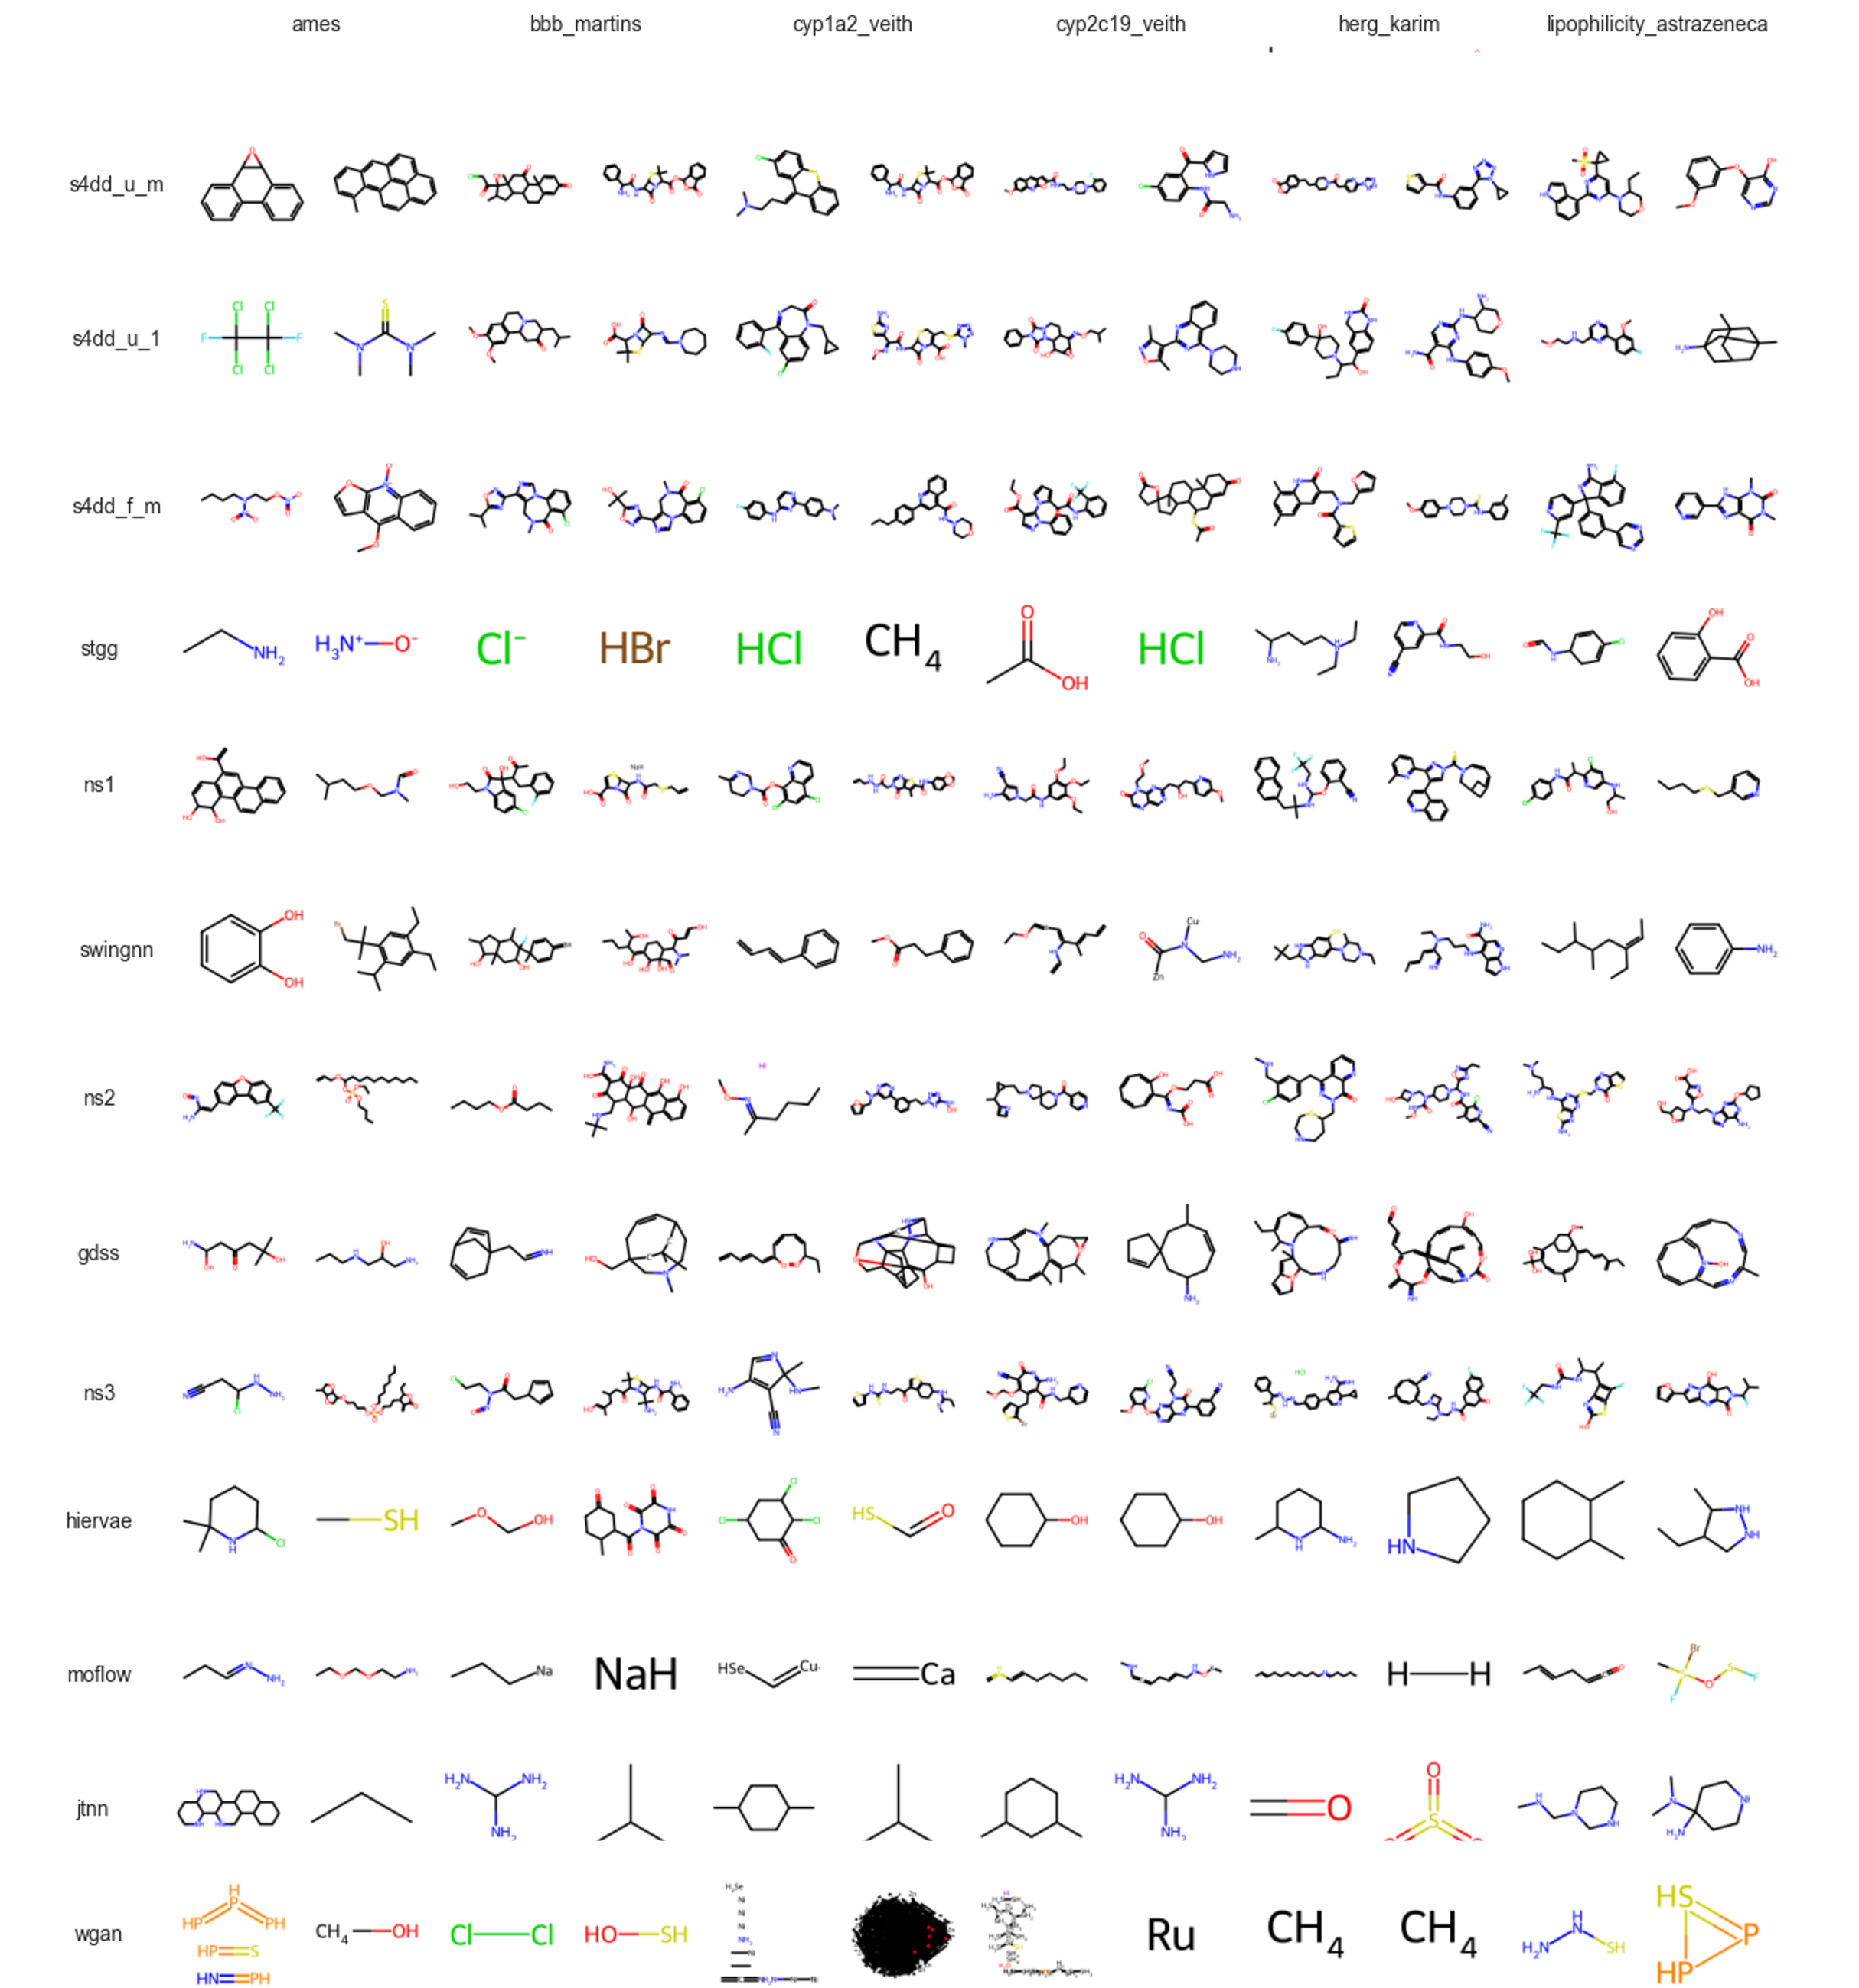
\includegraphics[width=\textwidth]{images/rankgen/real_generators/generated_molecules.png}
    \caption{Examples of molecules generated by different models across the six datasets. Each row is a generator; each dataset contributes a positive and a negative sample.}
    \label{fig:generated_molecules}
\end{figure}

\begin{figure}[H]
  \centering
  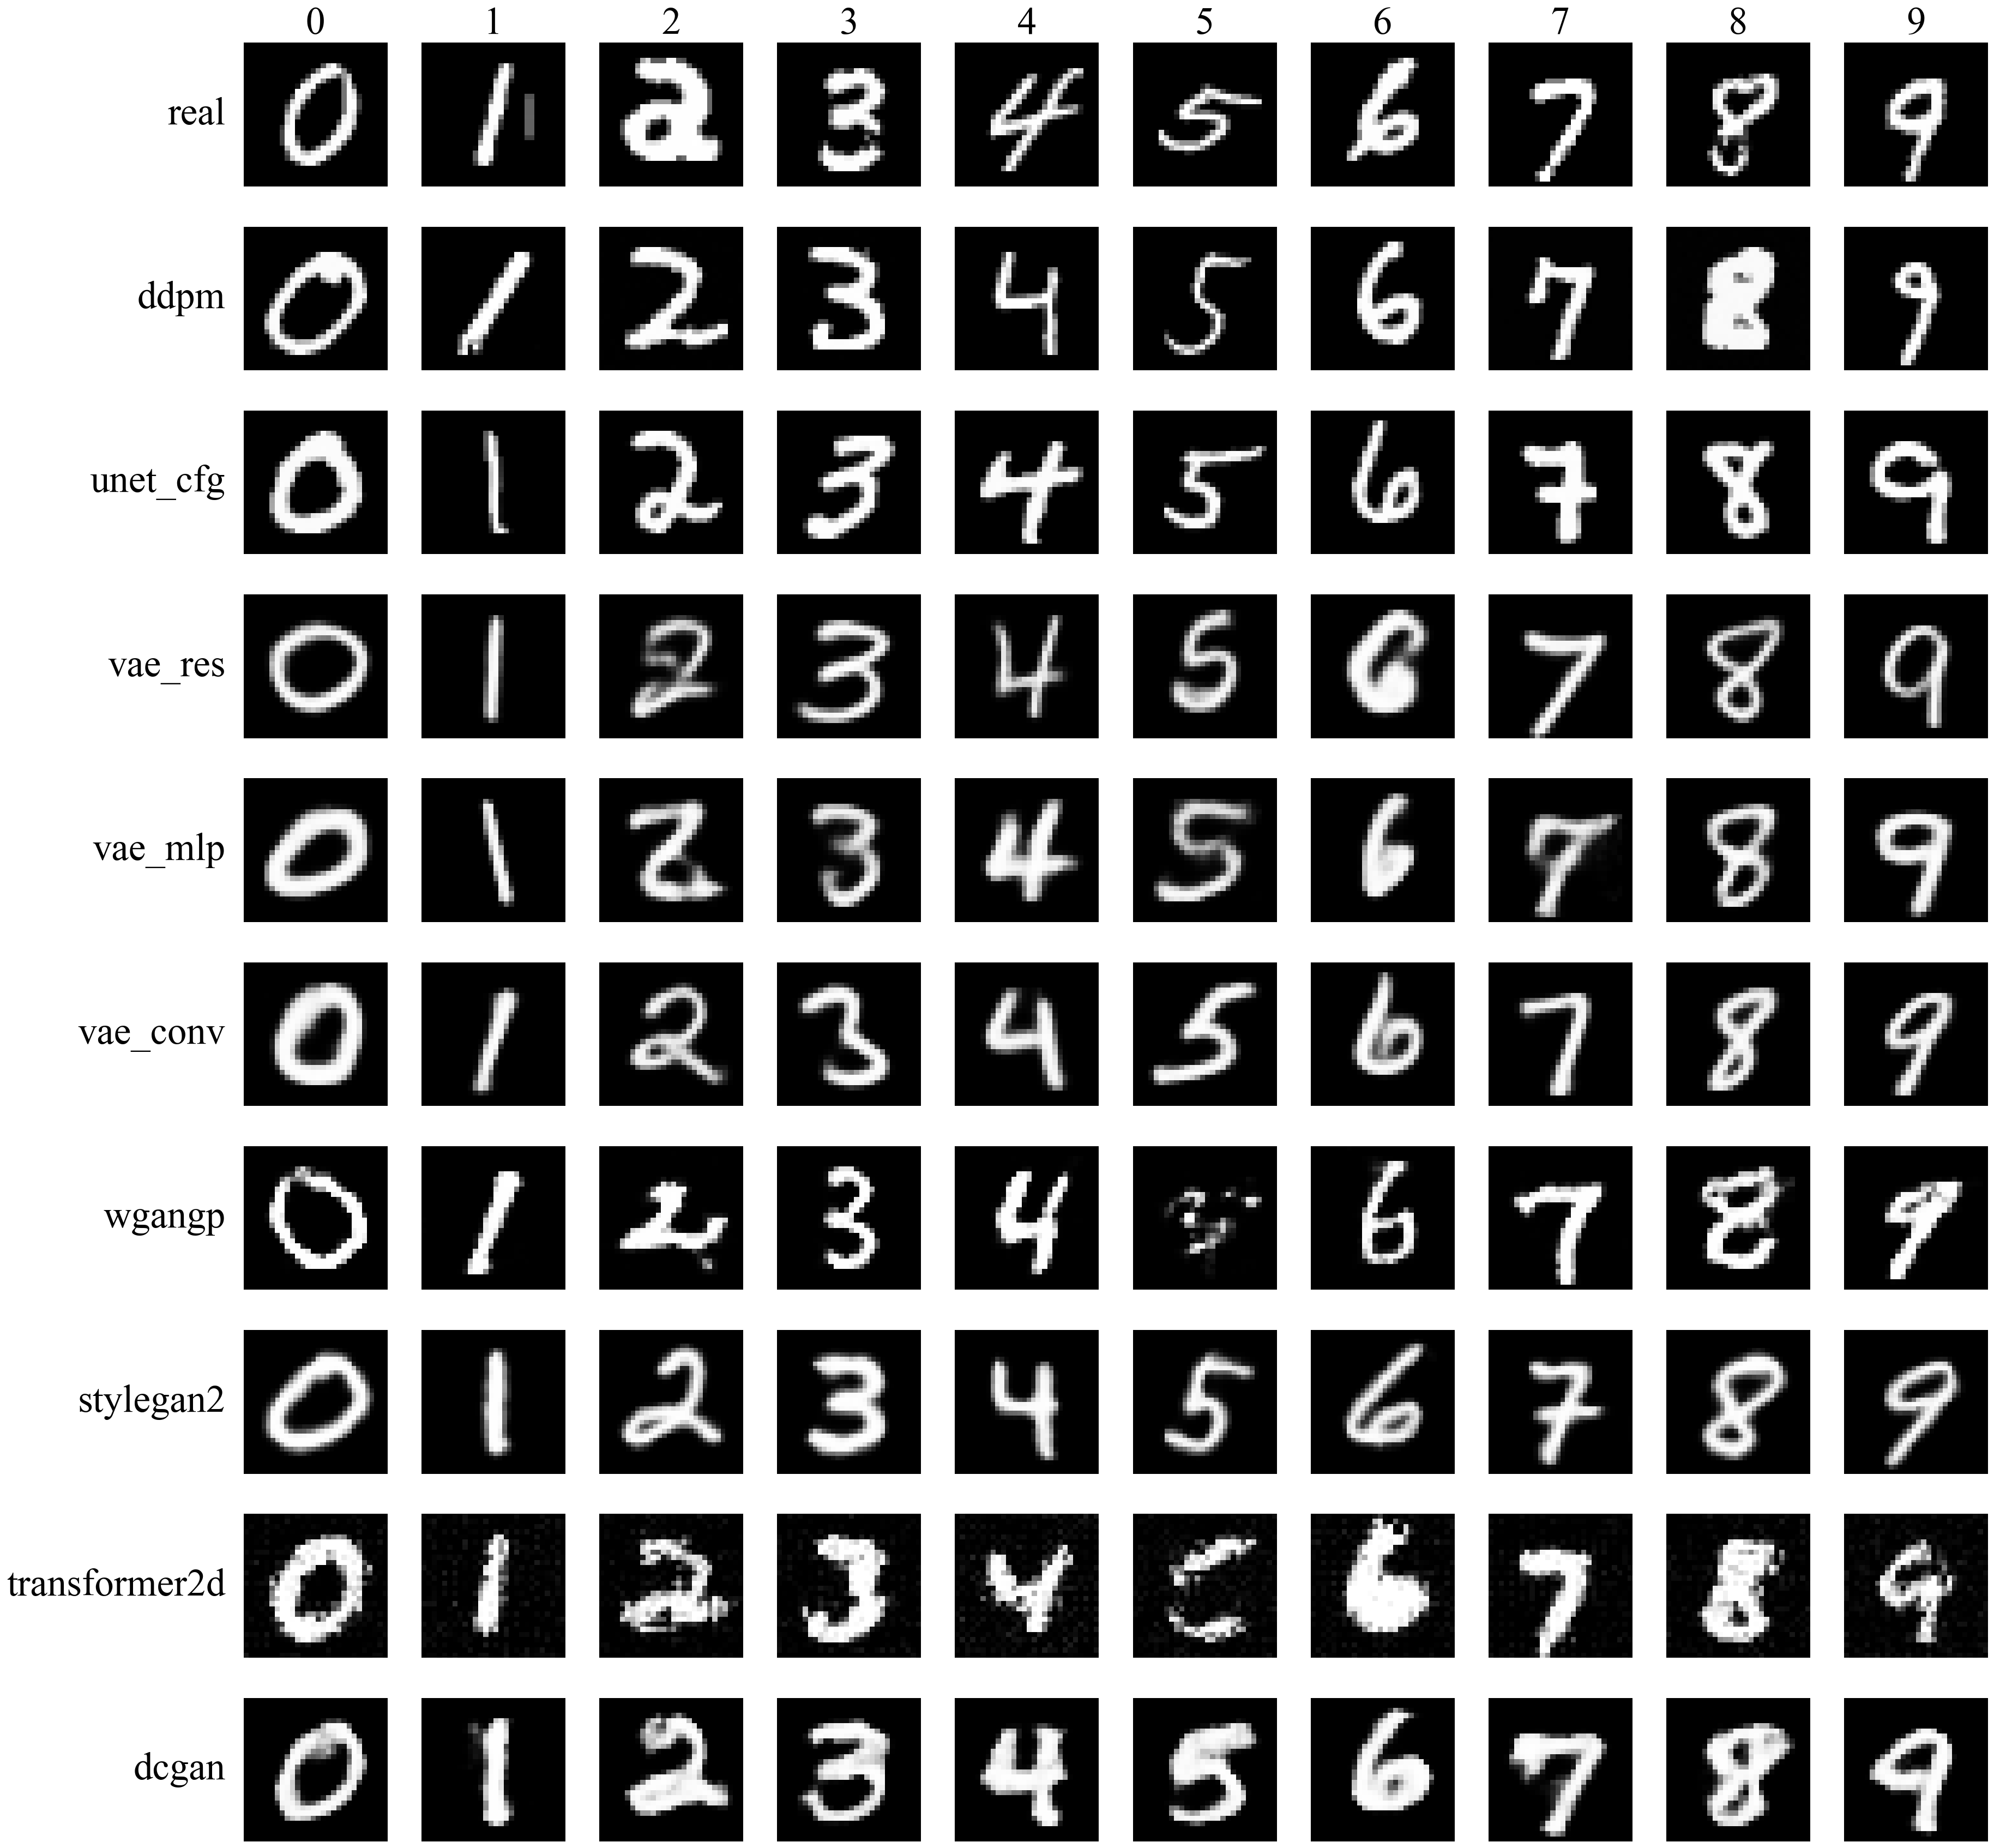
\includegraphics[width=\textwidth]{images/rankgen/real_generators/mnist_train1_generators_panel.png}
  \caption{Samples generated by each model on \textbf{MNIST}. Rows: generators; columns: class-conditional samples (uncurated).}
  \label{fig:mnist_generated_panel}
\end{figure}

\begin{figure}[H]
  \centering
  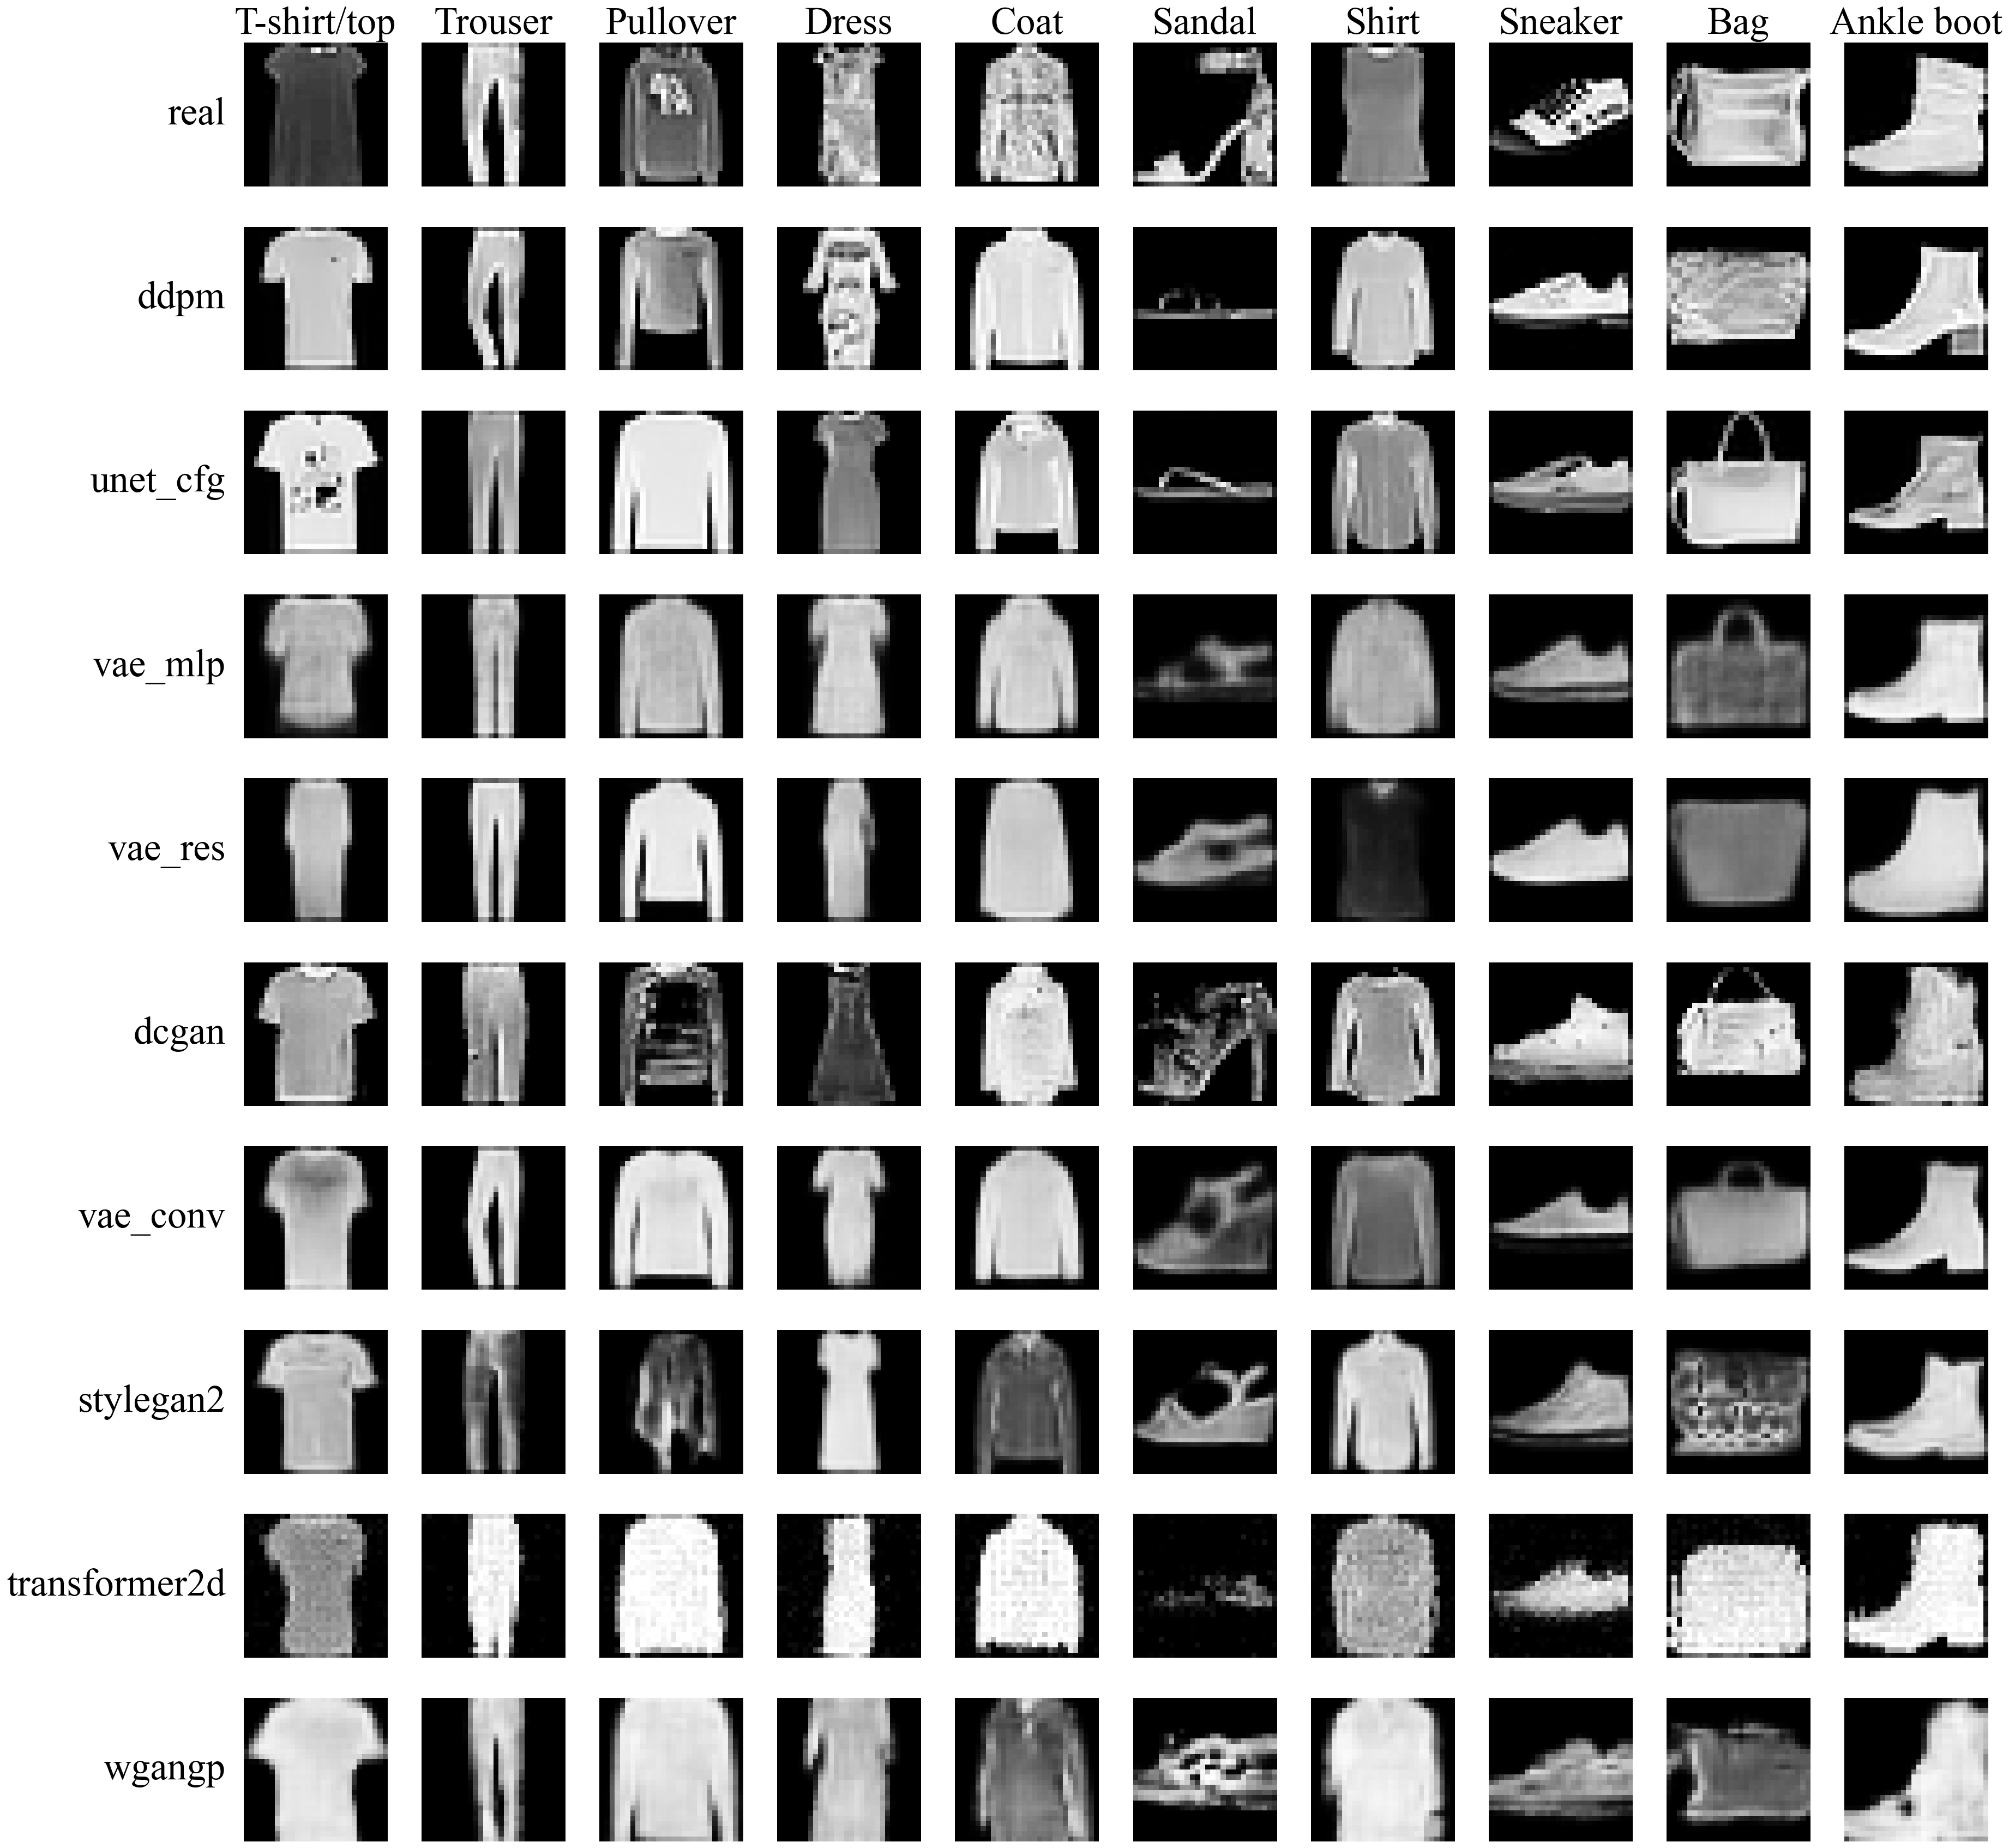
\includegraphics[width=\textwidth]{images/rankgen/real_generators/fashionmnist_train1_generators_panel.png}
  \caption{Samples generated by each model on \textbf{Fashion\textendash MNIST}. Rows: generators; columns: class-conditional samples (uncurated).}
  \label{fig:fashionmnist_generated_panel}
\end{figure}

\begin{figure}[H]
  \centering
  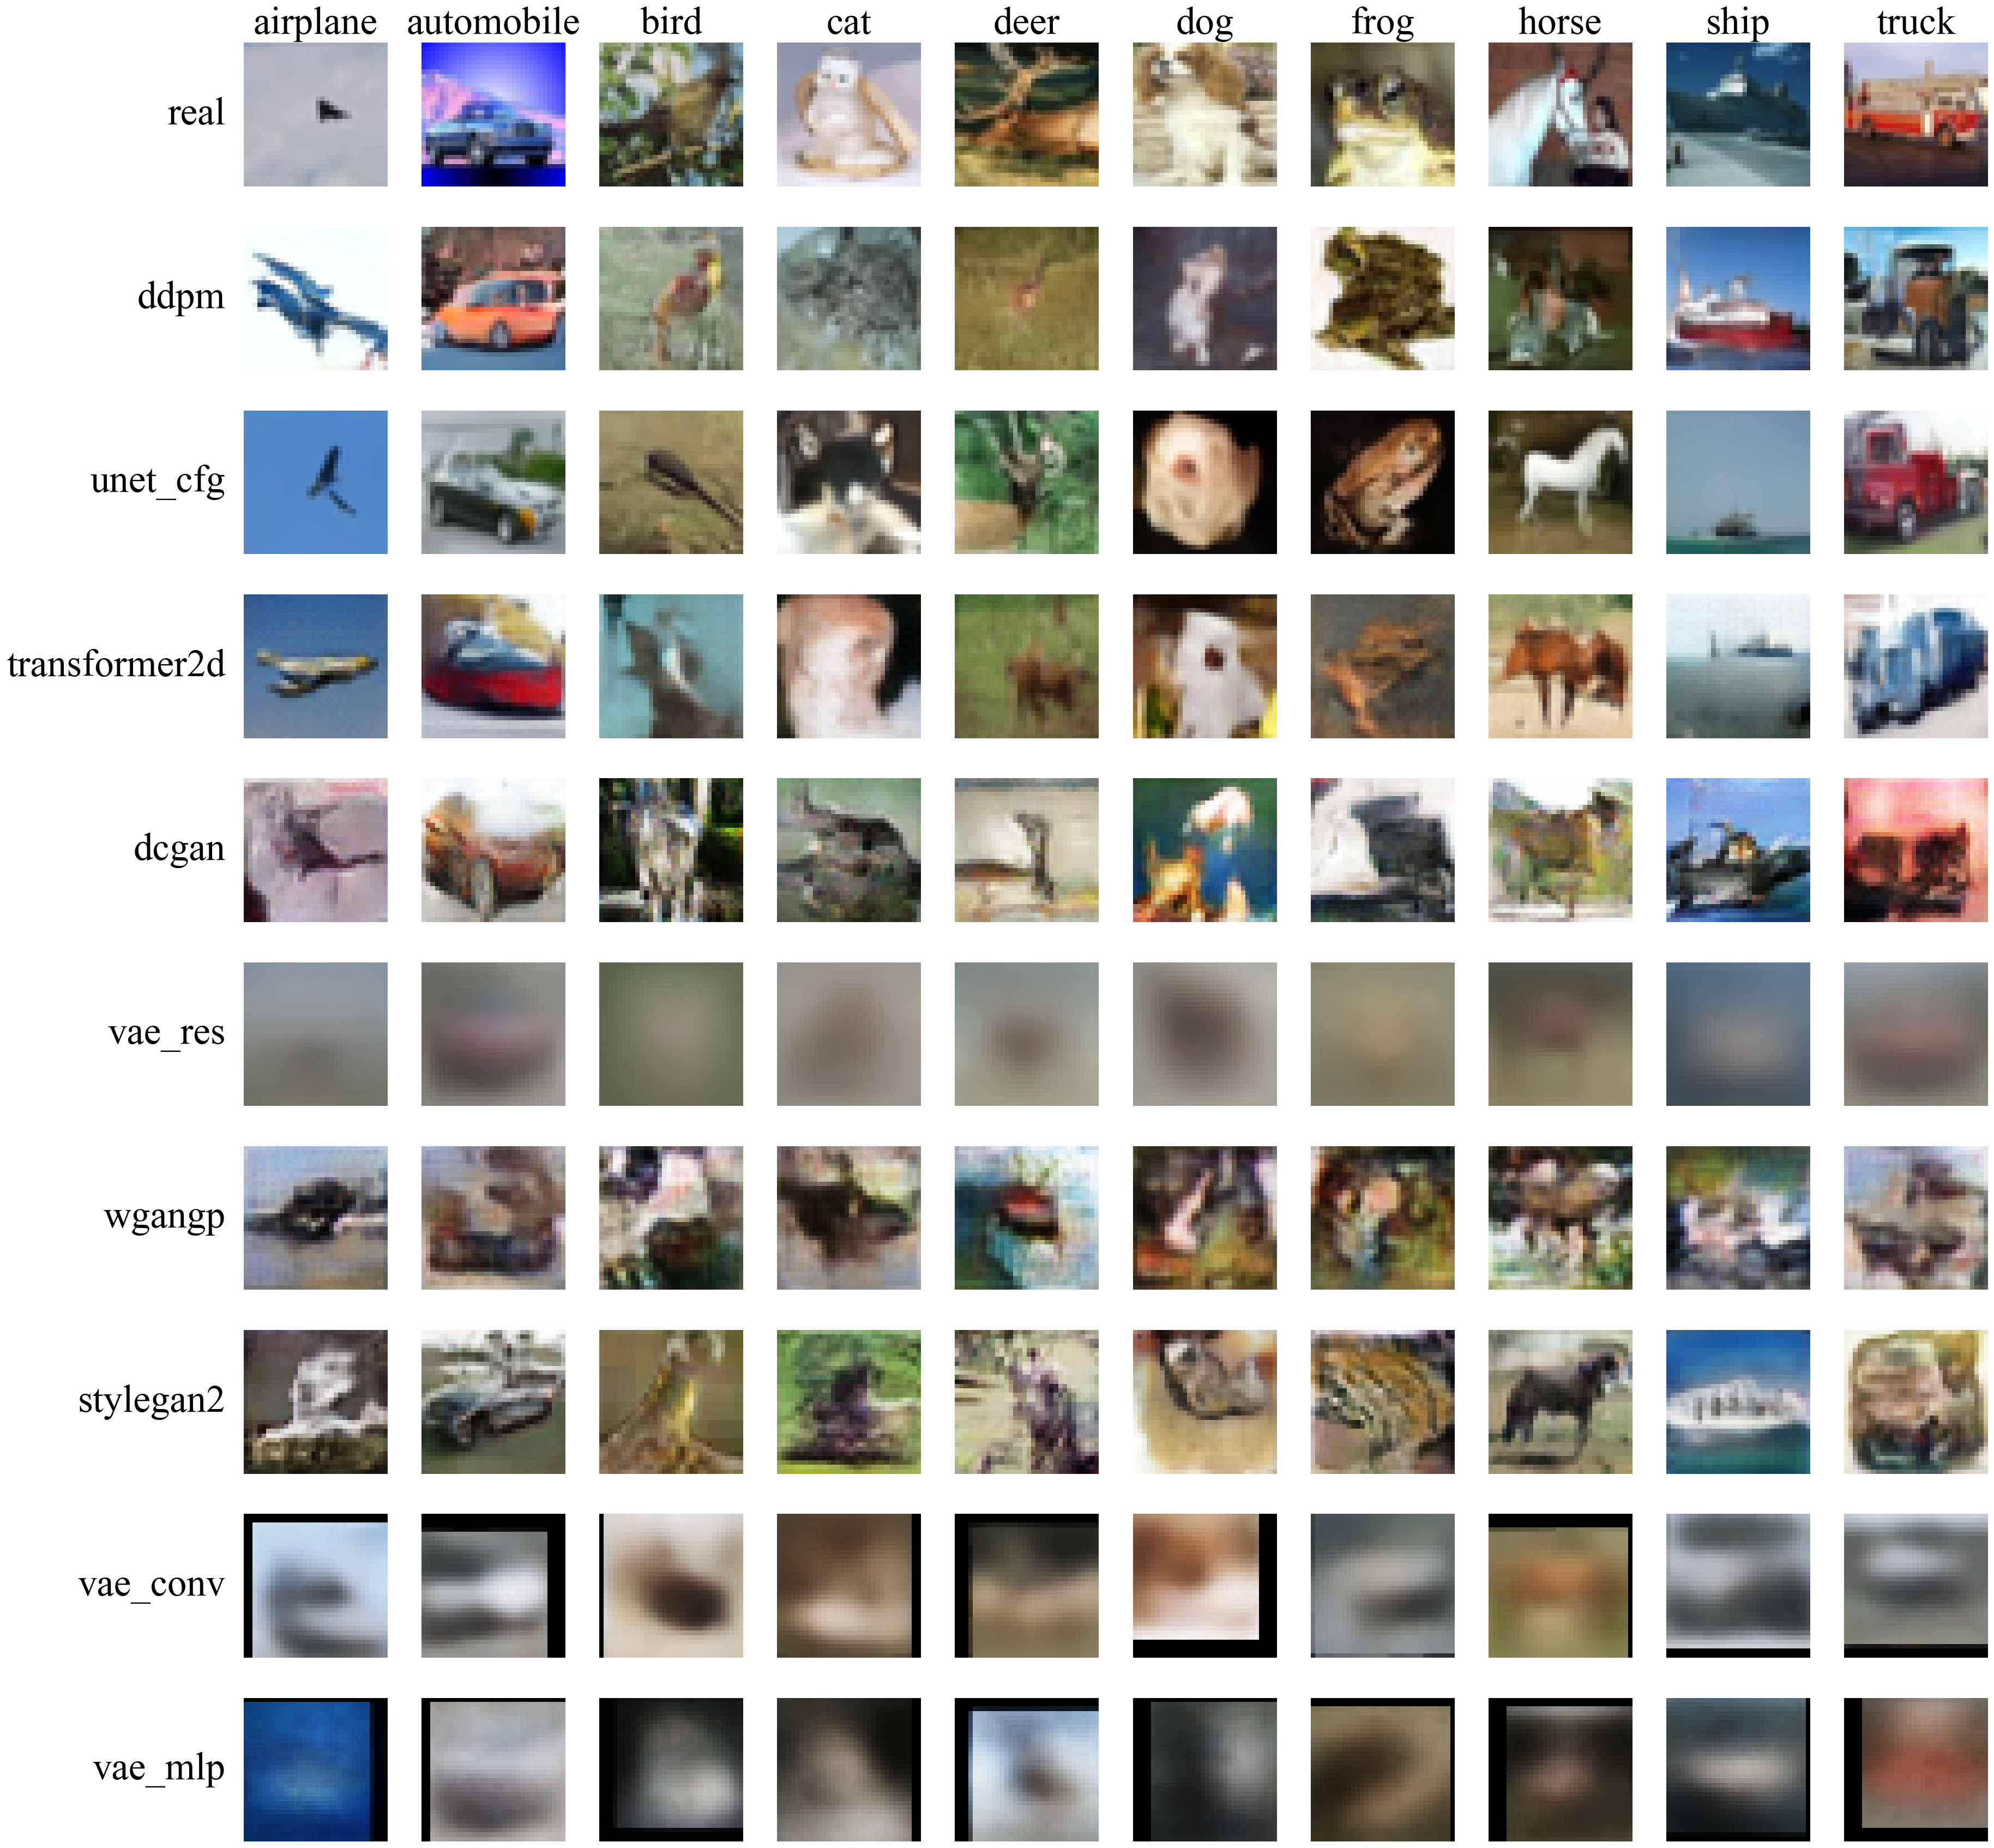
\includegraphics[width=\textwidth]{images/rankgen/real_generators/cifar10_train1_generators_panel.png}
  \caption{Samples generated by each model on \textbf{CIFAR\textendash 10}. Rows: generators; columns: per-class conditional samples (uncurated).}
  \label{fig:cifar10_generated_panel}
\end{figure}

\section{Precision, Recall, Density, and Coverage Rank of Real Generators}
\label{appendix:pr_dc_alternative_rank}
\begin{figure}[H]
  \centering
  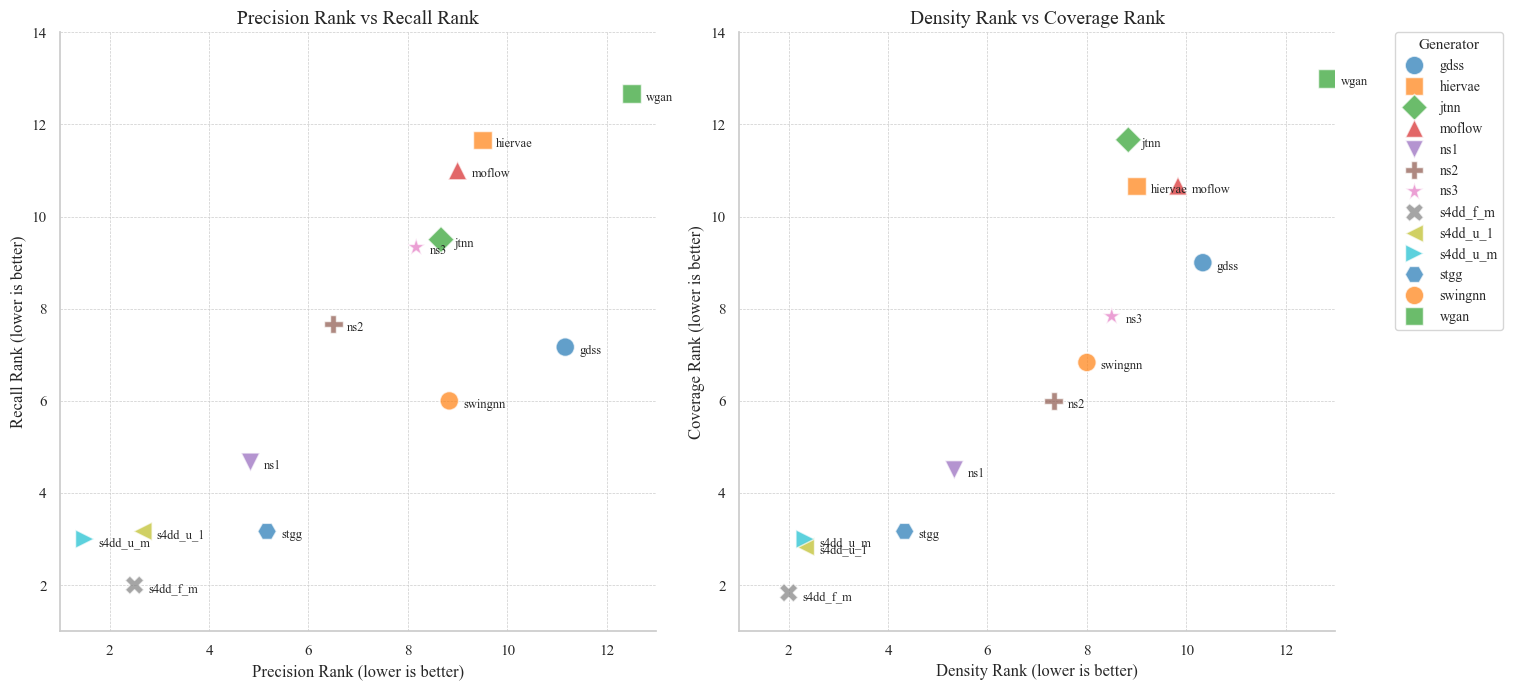
\includegraphics[width=0.75\linewidth]{images/rankgen/real_generators/generators_rank_pr.png}
  \caption{Rank comparisons of real graph generators: Precision vs.\ Recall (left) and Density vs.\ Coverage (right). Lower rank is better.}
  \label{fig:rank_pr_dc}
\end{figure}

\section{Robustness of Alternative Metrics to Data Perturbations}
\label{appendix:pr_dc}
\begin{figure}[H]
  \centering
  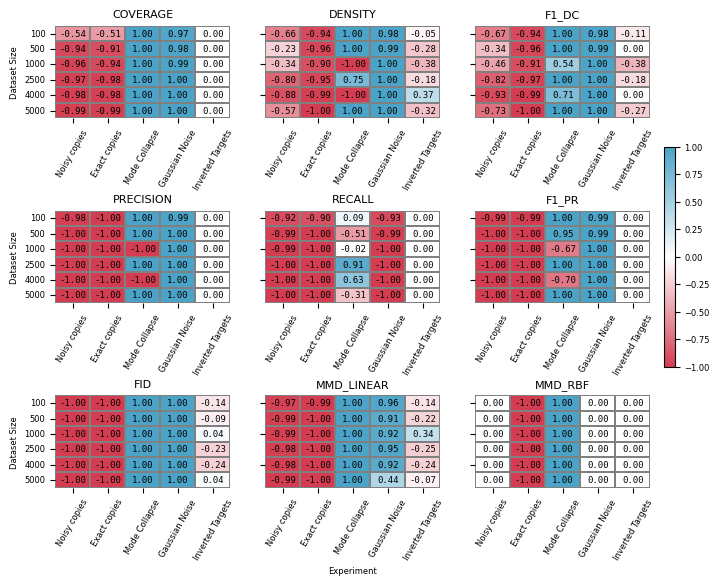
\includegraphics[width=1.0\linewidth]{images/rankgen/synthetic/pr_dc_1.png}
  \caption{Effect of perturbations on Coverage, Density, F1-DC, Precision, Recall, F1-PR, FID, MMD\_Linear, MMD\_RBF across dataset sizes.}
  \label{fig:metric_pr_dc_perturb}
\end{figure}

Despite broad use, many alternative metrics show limited robustness to perturbations; e.g., MMD\_RBF is nearly unchanged under noisy copies.

\section{Real-World Dataset Generation Experiments in Detail}
\section{Average Rank per Dataset for Each Vectorizer}

\subsection{AMES}
\begin{figure}[H]
  \centering
  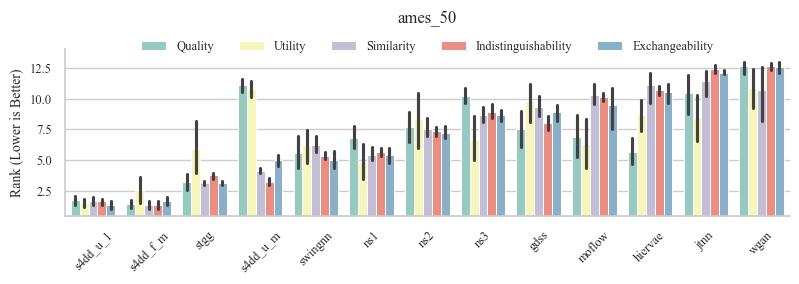
\includegraphics[width=1.0\linewidth]{images/rankgen/real_generators/generators_rank_ames.png}
  \caption{Average generator rank on \textbf{AMES} across vectorizers (lower is better).}
  \label{fig:rank_ames}
\end{figure}

\subsection{BBB Martins}
\begin{figure}[H]
  \centering
  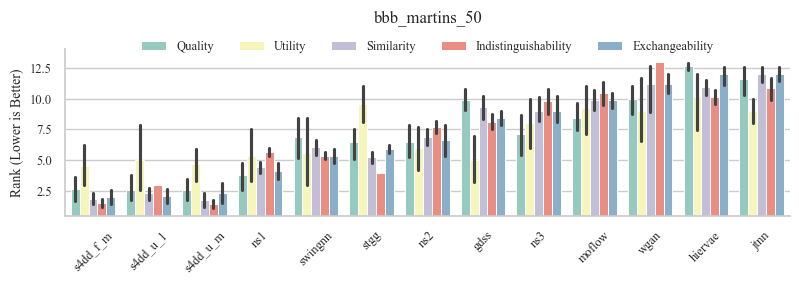
\includegraphics[width=1.0\linewidth]{images/rankgen/real_generators/generators_rank_bbb_martins.png}
  \caption{Average generator rank on \textbf{BBB Martins} across vectorizers (lower is better).}
  \label{fig:rank_bbb}
\end{figure}

\subsection{CYP1A2}
\begin{figure}[H]
  \centering
  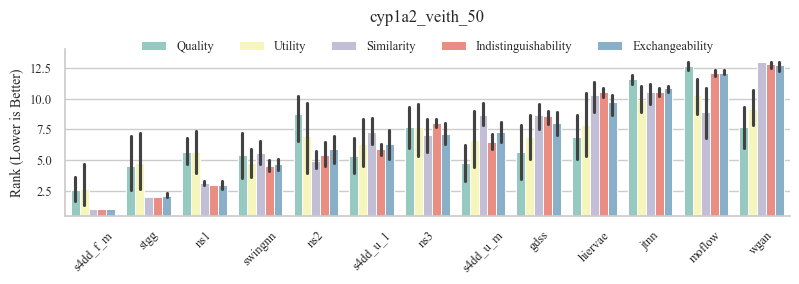
\includegraphics[width=1.0\linewidth]{images/rankgen/real_generators/generators_rank_cyp1a2.png}
  \caption{Average generator rank on \textbf{CYP1A2} across vectorizers (lower is better).}
  \label{fig:rank_cypa12}
\end{figure}

\subsection{CYP2C19}
\begin{figure}[H]
  \centering
  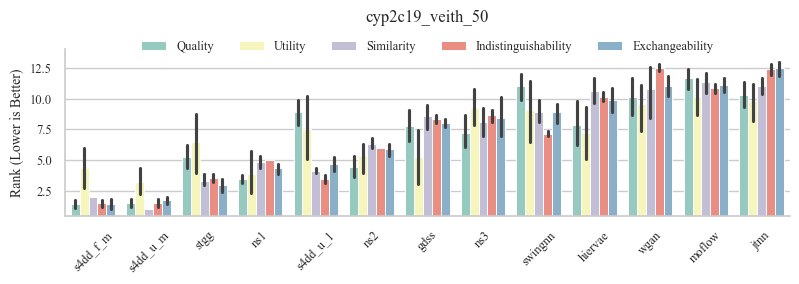
\includegraphics[width=1.0\linewidth]{images/rankgen/real_generators/generators_rank_cyp2c19.png}
  \caption{Average generator rank on \textbf{CYP2C19} across vectorizers (lower is better).}
  \label{fig:rank_cyp2c19}
\end{figure}

\subsection{hERG Karim}
\begin{figure}[H]
  \centering
  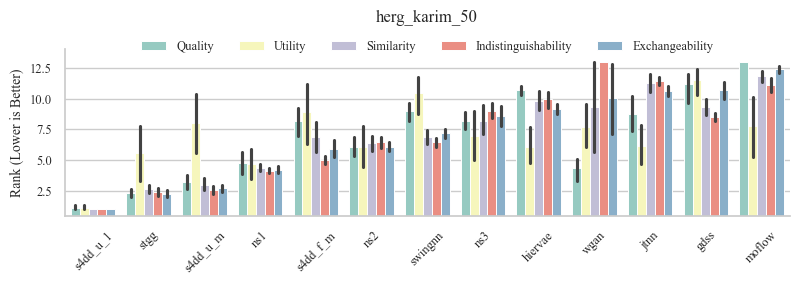
\includegraphics[width=1.0\linewidth]{images/rankgen/real_generators/generators_rank_herk_karim.png}
  \caption{Average generator rank on \textbf{hERG Karim} across vectorizers (lower is better).}
  \label{fig:rank_herg_karim}
\end{figure}

\subsection{Lipophilicity AstraZeneca}

\begin{figure}[htbp] % safer than [H]
  \centering
  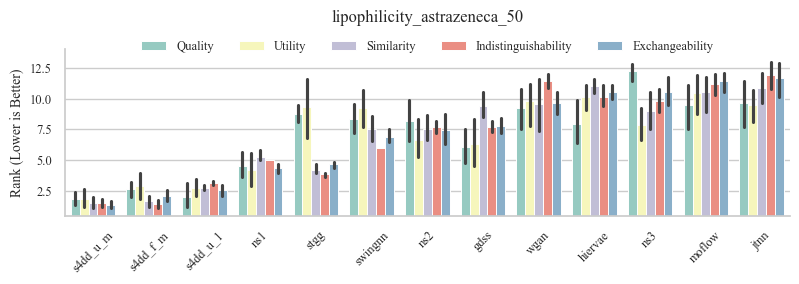
\includegraphics[width=\linewidth]{images/rankgen/real_generators/generators_rank_lipo.png}
  \caption{Average generator rank on \textbf{Lipophilicity AstraZeneca} across vectorizers (lower is better).}
  \label{fig:rank_Lipophilicity_Astrazeneca}
\end{figure}
\section{Image-Domain Experiments: Datasets, Models, and Full Results}
\label{app:image-experiments}
% (Shared preprocessing and split policy retained.)

\section{Datasets, Preprocessing, and Splits}
\label{app:image-data}
\begin{table}[H]
\centering
\scriptsize
\caption{Shared preprocessing and canonical splits used for all models and experiments.}
\label{tab:img-data-shared}
\begin{adjustbox}{max width=\linewidth}
\begin{tabular}{@{}lcccc@{}}
\toprule
Dataset & Shape $(C\times H\times W)$ & Pixel scale & Default train aug. & Split policy \\
\midrule
MNIST & $1\times28\times28$ & $[-1,1]$ from $[0,1]$ & none & stratified 50/50 \texttt{train1}/\texttt{train2} (seed 42); test untouched \\
FashionMNIST & $1\times28\times28$ & $[-1,1]$ & none & same \\
CIFAR-10 & $3\times32\times32$ & $[-1,1]$ & none$^\dagger$ & same \\
\bottomrule
\end{tabular}
\end{adjustbox}

\vspace{2pt}\footnotesize $^\dagger$ Some models enable flip/crop at training time; exports match dataset size.
\end{table}

% (Model/training tables retained; minor wording normalized.)

\section{Image Data Full Metric Results Tables}
\label{app:image-results}

% --- CIFAR-10 ---
\begin{table}[H]\centering\scriptsize
\caption{Metric values (left) and ranks (right) on \textbf{CIFAR-10}. Lower rank is better.}
\label{tab:vals-ranks-cifar10}
\begin{tabular}{l rr rr rr rr rr}
\toprule
\multirow{2}{*}{\textbf{Generator}} & \multicolumn{2}{c}{\textbf{Q}} & \multicolumn{2}{c}{\textbf{U}} & \multicolumn{2}{c}{\textbf{S}} & \multicolumn{2}{c}{\textbf{I}} & \multicolumn{2}{c}{\textbf{E}} \\
 & \textit{val} & \textit{rank} & \textit{val} & \textit{rank} & \textit{val} & \textit{rank} & \textit{val} & \textit{rank} & \textit{val} & \textit{rank} \\
\midrule
DCGAN & 0.670 & 9.0 & 0.000 & 6.5 & 0.450 & 4.0 & 0.450 & 1.0 & 0.150 & 4.0 \\
DDPM & 0.940 & 2.5 & 0.250 & 3.0 & 0.550 & 1.0 & 0.430 & 2.0 & 0.290 & 1.0 \\
StyleGAN2 & 0.880 & 4.0 & 0.000 & 6.5 & 0.190 & 9.0 & 0.080 & 6.0 & 0.060 & 7.0 \\
Transformer2D & 0.950 & 1.0 & 0.290 & 1.0 & 0.510 & 3.0 & 0.400 & 4.0 & 0.280 & 3.0 \\
UNet\_CFG & 0.940 & 2.5 & 0.250 & 2.0 & 0.530 & 2.0 & 0.410 & 3.0 & 0.280 & 2.0 \\
VAE\_Conv & 0.760 & 6.0 & 0.000 & 6.5 & 0.230 & 7.0 & 0.010 & 7.5 & 0.050 & 8.0 \\
VAE\_MLP & 0.740 & 7.0 & 0.000 & 6.5 & 0.210 & 8.0 & 0.010 & 7.5 & 0.040 & 9.0 \\
VAE\_Res & 0.770 & 5.0 & 0.000 & 6.5 & 0.400 & 5.0 & 0.000 & 9.0 & 0.080 & 5.5 \\
WGAN-GP & 0.720 & 8.0 & 0.000 & 6.5 & 0.280 & 6.0 & 0.140 & 5.0 & 0.080 & 5.5 \\
\bottomrule
\end{tabular}
\end{table}

% --- Fashion-MNIST ---
\begin{table}[H]\centering\scriptsize
\caption{Metric values (left) and ranks (right) on \textbf{Fashion-MNIST}. Lower rank is better.}
\label{tab:vals-ranks-fashionmnist}
\begin{tabular}{l rr rr rr rr rr}
\toprule
\multirow{2}{*}{\textbf{Generator}} & \multicolumn{2}{c}{\textbf{Q}} & \multicolumn{2}{c}{\textbf{U}} & \multicolumn{2}{c}{\textbf{S}} & \multicolumn{2}{c}{\textbf{I}} & \multicolumn{2}{c}{\textbf{E}} \\
 & \textit{val} & \textit{rank} & \textit{val} & \textit{rank} & \textit{val} & \textit{rank} & \textit{val} & \textit{rank} & \textit{val} & \textit{rank} \\
\midrule
DCGAN & 0.930 & 5.5 & 0.020 & 1.0 & 0.300 & 6.0 & 0.100 & 3.0 & 0.090 & 5.5 \\
DDPM & 0.940 & 2.5 & 0.000 & 5.5 & 0.500 & 1.5 & 0.170 & 1.0 & 0.160 & 1.0 \\
StyleGAN2 & 0.940 & 2.5 & 0.000 & 5.5 & 0.220 & 7.0 & 0.000 & 7.0 & 0.050 & 7.0 \\
Transformer2D & 0.810 & 8.0 & 0.000 & 5.5 & 0.060 & 8.0 & 0.000 & 7.0 & 0.010 & 8.5 \\
UNet\_CFG & 0.940 & 2.5 & 0.000 & 5.5 & 0.500 & 1.5 & 0.140 & 2.0 & 0.150 & 2.0 \\
VAE\_Conv & 0.920 & 7.0 & 0.000 & 5.5 & 0.400 & 5.0 & 0.000 & 7.0 & 0.090 & 5.5 \\
VAE\_MLP & 0.940 & 2.5 & 0.000 & 5.5 & 0.430 & 3.5 & 0.000 & 7.0 & 0.100 & 3.5 \\
VAE\_Res & 0.930 & 5.5 & 0.000 & 5.5 & 0.430 & 3.5 & 0.000 & 7.0 & 0.100 & 3.5 \\
WGAN-GP & 0.790 & 9.0 & 0.000 & 5.5 & 0.050 & 9.0 & 0.010 & 4.0 & 0.010 & 8.5 \\
\bottomrule
\end{tabular}
\end{table}
% ===== MNIST =====
\begin{table}[h]\centering\scriptsize
\caption{Metric values (left) and ranks (right) on \textbf{MNIST}. Lower rank is better.}
\label{tab:vals-ranks-mnist}
\begin{tabular}{l rr rr rr rr rr}
\toprule
\multirow{2}{*}{\textbf{Generator}} & \multicolumn{2}{c}{\textbf{Q}} & \multicolumn{2}{c}{\textbf{U}} & \multicolumn{2}{c}{\textbf{S}} & \multicolumn{2}{c}{\textbf{I}} & \multicolumn{2}{c}{\textbf{E}} \\
 & \textit{val} & \textit{rank} & \textit{val} & \textit{rank} & \textit{val} & \textit{rank} & \textit{val} & \textit{rank} & \textit{val} & \textit{rank} \\
\midrule
dcgan         & 0.560 & 9.0 & 0.000 & 7.0 & 0.010 & 9.0 & 0.000 & 6.0 & 0.000 & 9.0 \\
ddpm          & 0.970 & 3.0 & 0.000 & 7.0 & 0.570 & 2.0 & 0.130 & 1.5 & 0.170 & 1.5 \\
stylegan2     & 0.920 & 7.0 & 0.090 & 1.0 & 0.090 & 7.0 & 0.060 & 6.0 & 0.020 & 7.0 \\
transformer2d & 0.820 & 8.0 & 0.000 & 7.0 & 0.070 & 8.0 & 0.000 & 6.0 & 0.020 & 8.0 \\
unet\_cfg     & 0.970 & 3.0 & 0.000 & 7.0 & 0.580 & 1.0 & 0.130 & 1.5 & 0.170 & 1.5 \\
vae\_conv     & 0.960 & 6.0 & 0.000 & 7.0 & 0.480 & 5.0 & 0.000 & 6.0 & 0.110 & 5.0 \\
vae\_mlp      & 0.970 & 3.0 & 0.000 & 7.0 & 0.490 & 4.0 & 0.000 & 6.0 & 0.120 & 4.0 \\
vae\_res      & 0.970 & 3.0 & 0.000 & 4.0 & 0.520 & 3.0 & 0.000 & 6.0 & 0.130 & 3.0 \\
wgangp        & 0.970 & 3.0 & 0.090 & 2.0 & 0.400 & 6.0 & 0.000 & 6.0 & 0.110 & 6.0 \\
\bottomrule
\end{tabular}
\end{table}

% --- CIFAR-10 (FID/KID/PR/IS) ---
\begin{table}[H]
\centering
\small
\caption{CIFAR-10 metrics with per-metric ranks ($r{=}1$ best). $n_{\text{ref}}{=}25{,}000$, $n_{\text{gen}}{=}25{,}000$.}
\label{tab:cifar10-ranked}
\begin{tabular}{lrrrrrrrrrrrr}
\toprule
\textbf{Model} & \textbf{FID} $\downarrow$ & \textbf{r} & \textbf{KID} $\downarrow$ & \textbf{r} & \textbf{P} & \textbf{r} & \textbf{R} & \textbf{r} & \textbf{F1\_pr} & \textbf{r} & \textbf{IS} & \textbf{r} \\
\midrule
DCGAN         & 21.62 & 5 & 0.0171 & 5 & 0.165 & 6 & 0.078 & 3 & 0.106 & 3 & 2.041 & 1 \\
DDPM          &  6.67 & 1 & 0.0030 & 1 & 0.224 & 3 & 0.122 & 1 & 0.158 & 1 & 2.017 & 2 \\
StyleGAN2     & 19.26 & 3 & 0.0129 & 3 & 0.220 & 4 & 0.002 & 6 & 0.005 & 6 & 1.958 & 3 \\
UNet\_CFG     &  9.62 & 2 & 0.0069 & 2 & 0.288 & 1 & 0.093 & 2 & 0.141 & 2 & 1.944 & 4 \\
Transformer2D & 20.13 & 4 & 0.0150 & 4 & 0.286 & 2 & 0.065 & 4 & 0.106 & 3 & 1.763 & 5 \\
VAE\_Conv     & 182.67 & 7 & 0.1905 & 7 & 0.110 & 7 & 0.000 & 7 & 0.000 & 7 & 1.293 & 7 \\
VAE\_MLP      & 206.49 & 8 & 0.2182 & 8 & 0.094 & 8 & 0.000 & 7 & 0.000 & 7 & 1.280 & 8 \\
VAE\_Res      & 374.51 & 9 & 0.4439 & 9 & 0.002 & 9 & 0.000 & 7 & 0.000 & 7 & 1.006 & 9 \\
WGAN-GP        &  42.62 & 6 & 0.0342 & 6 & 0.207 & 5 & 0.017 & 5 & 0.032 & 5 & 1.652 & 6 \\
\bottomrule
\end{tabular}
\end{table}

% --- Fashion-MNIST (FID/KID/PR/IS) ---
\begin{table}[H]
\centering
\small
\caption{Fashion-MNIST metrics with per-metric ranks ($r{=}1$ best). $n_{\text{ref}}{=}30{,}000$, $n_{\text{gen}}{=}30{,}000$.}
\label{tab:fashionmnist-ranked}
\begin{tabular}{lrrrrrrrrrrrr}
\toprule
\textbf{Model} & \textbf{FID} $\downarrow$ & \textbf{r} & \textbf{KID} $\downarrow$ & \textbf{r} & \textbf{P} & \textbf{r} & \textbf{R} & \textbf{r} & \textbf{F1\_pr} & \textbf{r} & \textbf{IS} & \textbf{r} \\
\midrule
DCGAN         & 0.19 & 1 & 0.0106 & 4 & 0.215 & 7 & 0.174 & 3 & 0.192 & 3 & 2.364 & 1 \\
DDPM          & 0.71 & 2 & 0.0018 & 1 & 0.369 & 2 & 0.246 & 1 & 0.295 & 1 & 1.994 & 3 \\
StyleGAN2     & 1.45 & 4 & 0.0077 & 3 & 0.318 & 3 & 0.001 & 8 & 0.002 & 8 & 1.869 & 5 \\
UNet\_CFG     & 1.10 & 3 & 0.0042 & 2 & 0.463 & 1 & 0.188 & 2 & 0.268 & 2 & 1.905 & 4 \\
Transformer2D & 5.45 & 9 & 0.0587 & 9 & 0.090 & 8 & 0.001 & 8 & 0.002 & 8 & 1.570 & 9 \\
VAE\_Conv     & 3.82 & 6 & 0.0231 & 6 & 0.230 & 6 & 0.009 & 4 & 0.017 & 4 & 1.692 & 6 \\
VAE\_MLP      & 4.59 & 8 & 0.0216 & 5 & 0.252 & 5 & 0.007 & 5 & 0.014 & 5 & 1.677 & 7 \\
VAE\_Res      & 3.99 & 7 & 0.0257 & 7 & 0.257 & 4 & 0.006 & 6 & 0.011 & 6 & 1.673 & 8 \\
WGAN-GP        & 2.19 & 5 & 0.0423 & 8 & 0.057 & 9 & 0.005 & 7 & 0.009 & 7 & 2.013 & 2 \\
\bottomrule
\end{tabular}
\end{table}

% --- MNIST (FID/KID/PR/IS) ---
\begin{table}[H]
\centering
\small
\caption{MNIST metrics with per-metric ranks ($r{=}1$ best). $n_{\text{ref}}{=}30{,}000$, $n_{\text{gen}}{=}30{,}000$.}
\label{tab:mnist-ranked}
\begin{tabular}{lrrrrrrrrrrrr}
\toprule
\textbf{Model} & \textbf{FID} $\downarrow$ & \textbf{r} & \textbf{KID} $\downarrow$ & \textbf{r} & \textbf{P} & \textbf{r} & \textbf{R} & \textbf{r} & \textbf{F1\_pr} & \textbf{r} & \textbf{IS} & \textbf{r} \\
\midrule
DCGAN         & 3.89 & 9 & 0.0321 & 8 & 0.307 & 3 & 0.003 & 7 & 0.007 & 7 & 1.276 & 9 \\
DDPM          & 0.25 & 4 & 0.0016 & 1 & 0.488 & 2 & 0.319 & 1 & 0.386 & 1 & 1.634 & 7 \\
StyleGAN2     & 2.27 & 8 & 0.0144 & 6 & 0.291 & 4 & 0.000 & 9 & 0.000 & 9 & 1.478 & 8 \\
UNet\_CFG     & 0.29 & 5 & 0.0017 & 2 & 0.531 & 1 & 0.299 & 2 & 0.383 & 2 & 1.636 & 6 \\
Transformer2D & 0.83 & 7 & 0.1345 & 9 & 0.027 & 9 & 0.003 & 7 & 0.005 & 8 & 1.647 & 5 \\
VAE\_Conv     & 0.24 & 3 & 0.0114 & 3 & 0.223 & 5 & 0.072 & 5 & 0.109 & 5 & 1.784 & 3 \\
VAE\_MLP      & 0.23 & 2 & 0.0125 & 4 & 0.206 & 8 & 0.082 & 4 & 0.117 & 4 & 1.816 & 2 \\
VAE\_Res      & 0.40 & 6 & 0.0141 & 5 & 0.212 & 6 & 0.052 & 6 & 0.084 & 6 & 1.716 & 4 \\
WGAN-GP        & 0.14 & 1 & 0.0163 & 7 & 0.210 & 7 & 0.207 & 3 & 0.209 & 3 & 1.865 & 1 \\
\bottomrule
\end{tabular}
\end{table}

% --- Kernel-entropy diversity proxies (CIFAR-10) ---
\begin{table}[H]
\centering
\small
\caption{Kernel-entropy metrics on CIFAR-10 with per-metric ranks ($r{=}1$ best). Higher is better for RKE\_gen, FKEA-VENDI\_gen, FKEA-RKE2\_gen; lower is better for RRKE.}
\label{tab:ke-cifar10-ranked}
\begin{tabular}{lrrrrrrrrrrr}
\toprule
\textbf{Model} & $\boldsymbol{\sigma}$ & \textbf{RKE\_gen} & \textbf{r} & $\boldsymbol{\hat m}$ & \textbf{RRKE} & \textbf{r} & \textbf{FKEA-VENDI\_gen} & \textbf{r} & \textbf{FKEA-RKE2\_gen} & \textbf{r} \\
\midrule
DCGAN         & 15.18 & 0.852 & 5 & 2 & 0.179 & 5 & 13.1 & 3 & 2.3 & 3 \\
DDPM          & 15.72 & 0.942 & 1 & 3 & 0.120 & 1 & 15.7 & 1 & 2.6 & 1 \\
StyleGAN2     & 15.21 & 0.858 & 3 & 2 & 0.167 & 4 & 12.6 & 4 & 2.3 & 3 \\
UNet\_CFG     & 15.54 & 0.901 & 2 & 2 & 0.129 & 2 & 14.0 & 2 & 2.4 & 2 \\
Transformer2D & 15.28 & 0.855 & 4 & 2 & 0.165 & 3 & 12.4 & 5 & 2.4 & 2 \\
VAE\_Conv     & 15.34 & 0.335 & 7 & 1 & 0.762 & 7 &  2.8 & 7 & 1.4 & 5 \\
VAE\_MLP      & 15.54 & 0.305 & 8 & 1 & 0.829 & 8 &  2.5 & 8 & 1.4 & 5 \\
VAE\_Res      & 17.04 & 0.014 & 9 & 1 & 1.228 & 9 &  1.1 & 9 & 1.0 & 6 \\
WGAN-GP        & 14.82 & 0.745 & 6 & 2 & 0.249 & 6 &  9.5 & 6 & 2.1 & 4 \\
\bottomrule
\end{tabular}
\end{table}

% --- Kernel-entropy diversity proxies (Fashion-MNIST) ---
\begin{table}[H]
\centering
\small
\caption{Kernel-entropy metrics on Fashion-MNIST with per-metric ranks ($r{=}1$ best).}
\label{tab:ke-fashionmnist-ranked}
\begin{tabular}{lrrrrrrrrrrr}
\toprule
\textbf{Model} & $\boldsymbol{\sigma}$ & \textbf{RKE\_gen} & \textbf{r} & $\boldsymbol{\hat m}$ & \textbf{RRKE} & \textbf{r} & \textbf{FKEA-VENDI\_gen} & \textbf{r} & \textbf{FKEA-RKE2\_gen} & \textbf{r} \\
\midrule
DCGAN         & 16.63 & 0.953 & 1 & 3 & 0.120 & 3 & 14.7 & 1 & 2.6 & 1 \\
DDPM          & 16.56 & 0.945 & 2 & 3 & 0.083 & 1 & 13.1 & 2 & 2.6 & 1 \\
StyleGAN2     & 16.39 & 0.905 & 4 & 2 & 0.133 & 4 & 11.1 & 4 & 2.5 & 2 \\
UNet\_CFG     & 16.46 & 0.923 & 3 & 3 & 0.092 & 2 & 11.9 & 3 & 2.5 & 2 \\
Transformer2D & 16.62 & 0.848 & 7 & 2 & 0.357 & 9 &  8.7 & 9 & 2.3 & 4 \\
VAE\_Conv     & 16.19 & 0.852 & 6 & 2 & 0.205 & 6 &  9.3 & 6 & 2.3 & 4 \\
VAE\_MLP      & 16.26 & 0.852 & 6 & 2 & 0.199 & 5 &  9.0 & 8 & 2.3 & 4 \\
VAE\_Res      & 16.12 & 0.837 & 8 & 2 & 0.211 & 7 &  9.1 & 7 & 2.3 & 4 \\
WGAN-GP        & 16.54 & 0.879 & 5 & 2 & 0.263 & 8 & 10.6 & 5 & 2.4 & 3 \\
\bottomrule
\end{tabular}
\end{table}

% --- Kernel-entropy diversity proxies (MNIST) ---
\begin{table}[H]
\centering
\small
\caption{Kernel-entropy metrics on MNIST with per-metric ranks ($r{=}1$ best).}
\label{tab:ke-mnist-ranked}
\begin{tabular}{lrrrrrrrrrrr}
\toprule
\textbf{Model} & $\boldsymbol{\sigma}$ & \textbf{RKE\_gen} & \textbf{r} & $\boldsymbol{\hat m}$ & \textbf{RRKE} & \textbf{r} & \textbf{FKEA-VENDI\_gen} & \textbf{r} & \textbf{FKEA-RKE2\_gen} & \textbf{r} \\
\midrule
DCGAN         & 13.58 & 0.869 & 8 & 2 & 0.331 & 8 &  8.1 & 8 & 2.3 & 5 \\
DDPM          & 13.48 & 0.971 & 3 & 3 & 0.070 & 1 & 13.5 & 2 & 2.7 & 1 \\
StyleGAN2     & 13.21 & 0.882 & 7 & 2 & 0.235 & 7 &  8.7 & 7 & 2.4 & 4 \\
UNet\_CFG     & 13.40 & 0.972 & 2 & 3 & 0.071 & 2 & 13.0 & 3 & 2.6 & 2 \\
Transformer2D & 15.28 & 0.850 & 9 & 2 & 0.540 & 9 & 10.7 & 6 & 2.3 & 5 \\
VAE\_Conv     & 13.46 & 0.937 & 5 & 3 & 0.146 & 4 & 12.5 & 4 & 2.5 & 3 \\
VAE\_MLP      & 13.67 & 0.953 & 4 & 3 & 0.150 & 5 & 13.0 & 3 & 2.6 & 2 \\
VAE\_Res      & 13.38 & 0.921 & 6 & 3 & 0.161 & 6 & 11.9 & 5 & 2.5 & 3 \\
WGAN-GP        & 13.93 & 0.994 & 1 & 3 & 0.145 & 3 & 15.0 & 1 & 2.7 & 1 \\
\bottomrule
\end{tabular}
\end{table}


\paragraph{Relationship between RankGen and conventional metrics.}
Tables \ref{tab:vals-ranks-cifar10}--\ref{tab:vals-ranks-mnist}(RankGen metrics) and Tables~\ref{tab:cifar10-ranked}--\ref{tab:ke-mnist-ranked}(conventional metrics) show
that the two families of metrics agree at a coarse level but diverge in
precisely the situations where standard metrics are known to be unreliable.
Across CIFAR--10, Fashion--MNIST, and MNIST, diffusion models (DDPM, UNet--CFG)
rank near the top under both RankGen and baseline metrics such as
FID~\citep{heusel2017gans}, KID~\citep{binkowski2018demystifying},
precision/recall for distributions~\citep{sajjadi2018assessing,kynkaanniemi2019improved}
and Inception Score~\citep{salimans2016improved}, as well as
VENDI/RKE/FKEA kernel–entropy metrics~\citep{friedman2023vendi,pasarkar2024cousins,jalali2024fkea,luo2024converge}.
However, the generators that the conventional metrics disagree on are exactly
the ones where RankGen provides additional diagnostic resolution. For example,
StyleGAN2 achieves competitive FID/KID and very high precision but extremely low
recall, whereas RankGen penalizes it strongly through low Utility and low
Similarity, revealing its concentrated, mode-dropping behaviour. Conversely,
WGAN--GP obtains middling FID/KID but is classified by RankGen as having almost
zero Utility, correctly indicating that its samples add little task-relevant
information despite looking plausible in feature space. VAEs rank moderately
under FID/KID but RankGen identifies their weak task fidelity (low Quality) and
weak local mixing (low Indistinguishability), especially on CIFAR--10. Overall,
baseline metrics capture global similarity, while RankGen captures
\emph{task fidelity, augmentation value, local mixing, and copying}, explaining
the ranking discrepancies and providing complementary diagnostic information.




\section{Reproducibility Notes}
All experiments use seed $42$ unless otherwise stated. Evaluation uses equal $n_{\text{ref}}$ and $n_{\text{gen}}$ per dataset (see captions). 

\chapter{Record of Generative AI Use}
\label{app:ai-use}

This appendix records the use of generative AI tools during the preparation of
this thesis. Generative AI was used as an assistive tool for drafting support,
language refinement, structural editing, LaTeX troubleshooting, and consistency
checking. The intellectual contribution, research design, experiments,
interpretation of results, and final responsibility for the thesis remain with
the author.

\section{Summary of Use}

\begin{table}[H]
\centering
\small
\begin{tabularx}{\textwidth}{@{}p{0.24\textwidth}p{0.28\textwidth}X@{}}
\toprule
\textbf{Area of use} & \textbf{Purpose} & \textbf{Author oversight} \\
\midrule
Writing and editing & Assistance with wording, grammar, academic tone, and
paragraph restructuring. & All text was reviewed, revised, and accepted or
rejected by the author. \\
Thesis structure & Assistance with improving chapter framing, aims,
objectives, contribution statements, and conclusion structure. & The author
decided the final thesis structure and research claims. \\
LaTeX support & Assistance identifying LaTeX issues, appendix numbering
problems, glossary and notation consistency, and compilation blockers. & All
file changes were checked by the author before inclusion in the thesis. \\
Summarisation and consistency checking & Assistance comparing chapter content
against the abstract, introduction, conclusion, notation list, and
abbreviations. & The author verified the technical meaning and corrected the
final wording where necessary. \\
\bottomrule
\end{tabularx}
\caption{Summary of generative AI assistance used during thesis preparation.}
\label{tab:ai-use-summary}
\end{table}

\section{Declaration}

No generative AI tool was used as a substitute for conducting the research,
running experiments, producing original results, or making the final academic
judgements reported in this thesis. AI-assisted text was treated as draft
material only. The author reviewed and edited the final thesis content and
accepts responsibility for its accuracy, originality, and integrity.


% \include{appendix}
\end{document}
